% encoding: utf8
% !TEX encoding = utf8
% !TeX spellcheck = pl_PL

\documentclass[12pt,a4paper,titlepage, tikz]{book}

\usepackage{afterpage}
\usepackage{amsmath}
\usepackage{amssymb}
\usepackage[english,polish]{babel}
\usepackage{beramono}
\usepackage{bigstrut}
\usepackage{booktabs}
\usepackage{caption}
\usepackage{cite}
\usepackage{color}
\usepackage{enumitem}
\usepackage{epstopdf}
\usepackage{fancyhdr}
\usepackage{float}
\usepackage{perpage}
\usepackage[T1]{fontenc}
\usepackage{geometry}
\usepackage{gensymb}
\usepackage{graphicx}
\usepackage{hyperref}
\usepackage{indentfirst}
\usepackage[utf8]{inputenc}
\usepackage{listings}
\usepackage{leftidx}
\usepackage{lscape}
\usepackage{multirow}
\usepackage{pdfpages}
\usepackage{polski}
\usepackage{setspace}
\usepackage{subfigure}
\usepackage{textcomp}
\usepackage[mathcal]{euscript}

\usepackage{tikz}
\usepackage{textcomp}
\usetikzlibrary{shapes,arrows}


\usepackage{url}

\usepackage{verbatim}
\usepackage{rotating}
%\usepackage[section]{placeins}
\definecolor{gray}{rgb}{0.5,0.5,0.5}
\urlstyle{rm}

\lstset{
	backgroundcolor=\color{white},   % choose the background color; you must add \usepackage{color} or \usepackage{xcolor}
   	basicstyle=\footnotesize\ttfamily,        % the size of the fonts that are used for the code
   	breakatwhitespace=false,         % sets if automatic breaks should only happen at whitespace
   	breaklines=true,                 % sets automatic line breaking
   	captionpos=b,                    % sets the caption-position to bottom
   	commentstyle=\color{gray}\textit,    % comment style
   	deletekeywords={...},            % if you want to delete keywords from the given language
   	escapeinside=||,          % if you want to add LaTeX within your code
   	extendedchars=true,              % lets you use non-ASCII characters; for 8-bits encodings only, does not work with UTF-8
  	keepspaces=true,                 % keeps spaces in text, useful for keeping indentation of code (possibly needs columns=flexible)
   	language=Octave,                 % the language of the code
   	morekeywords={*,...},            % if you want to add more keywords to the set
   	numbers=left,                    % where to put the line-numbers; possible values are (none, left, right)
   	numbersep=5pt,                   % how far the line-numbers are from the code
   	numberstyle=\tiny\color{gray}, % the style that is used for the line-numbers
   	rulecolor=\color{black},         % if not set, the frame-color may be changed on line-breaks within not-black text (e.g. comments (green here))
   	showspaces=false,                % show spaces everywhere adding particular underscores; it overrides 'showstringspaces'
   	showstringspaces=false,          % underline spaces within strings only
   	showtabs=false,                  % show tabs within strings adding particular underscores
   	stepnumber=2,                    % the step between two line-numbers. If it's 1, each line will be numbered
 	tabsize=4,	                		% sets default tabsize
 	texcl=true
}

\clubpenalty=1000
\widowpenalty=1000
\brokenpenalty=1000
%\def\COMDIR{../../../common/}

\pagestyle{fancy} 
\fancyhf{}
\fancyhead[EL]{\textit{\textsc{\nouppercase{\leftmark}}}}
\fancyhead[OR]{\textit{\textsc{\nouppercase{\leftmark}}}}
\cfoot{}
\fancyfoot[EL]{\thepage}
\fancyfoot[OR]{\thepage}
\renewcommand{\headrulewidth}{0pt}
\renewcommand{\footrulewidth}{0pt}
\fancypagestyle{chapter}{\fancyhf{}\cfoot{}\fancyfoot[EL]{\thepage}\fancyfoot[OR]{\thepage}}
\fancypagestyle{plain}{\fancyfoot{}\fancyfoot[EL]{\thepage}\fancyfoot[OR]{\thepage}}

%\newcommand\blankpage{%
%    \null
%    \thispagestyle{empty}%
%    \addtocounter{page}{-1}%
%    \newpage}

\lstset{
basicstyle=\footnotesize\ttfamily,       	% the size of the fonts that are used for the code
	numbers=left,                   		% where to put the line-numbers
	numberstyle=\tiny\sffamily,      			% the size of the fonts that are used for the line-numbers
	stepnumber=1,                   		% the step between two line-numbers. If it's 1 each line will be numbered
	numbersep=8pt,                  		% how far the line-numbers are from the code
	showspaces=false,               		% show spaces adding particular underscores
	showstringspaces=false,         	% underline spaces within strings
	showtabs=false,                 		% show tabs within strings adding particular underscores
	tabsize=4,	                		% sets default tabsize
	captionpos=b,                   		% sets the caption-position
	breaklines=true,                		% sets automatic line breaking
	breakatwhitespace=true,        	% sets if automatic breaks should only happen at whitespace
	extendedchars=true,
	frame = l,
	xleftmargin=20pt,
	framexleftmargin=0pt,
	escapeinside=||,   
}

\frenchspacing
\sloppy
\geometry{verbose,a4paper,tmargin=2.5cm,bmargin=2.5cm,lmargin=3.5cm,rmargin=2.5cm}
\linespread{1.3}
\hyphenation{}
\begin{document}
\thispagestyle{empty}


% encoding: utf8
% !TEX encoding = utf8
% !TeX spellcheck = pl_PL

% STRONA TYTUŁOWA


\includepdf{pdf/strona_tytulowa.pdf}
\clearpage\mbox{}\thispagestyle{empty}\newpage


% AUTOR


%\par
%\vspace{0.2\baselineskip}
%\hfill\parbox{15em}{{\small\dotfill}\\[-.3ex]
%	\centerline{\footnotesize podpis studenta}}\par
%
%\vspace{1\baselineskip}

\clearpage\mbox{}\newpage


% STRESZCZENIE POLSKIE

\vspace*{\baselineskip}
\begin{center}
	{\large\bfseries Streszczenie}\par\bigskip
\end{center}
\noindent{\bf Tytuł}: {\itshape Kompensacja siły grawitacji związanej z chwytanym przedmiotem za pomocą regulatorów PID}
\\\\
{
	Zastosowanie siłowych praw sterowania daje możliwość łatwej kooperacji robota z~człowiekiem. Jednym z~nich jest sterowanie impedancyjne. W~trakcie manipulacji z~chwytaniem przedmiotów okazuje się, że siła grawitacji przedmiotu nie jest kompensowana przez silniki robota. Celem pracy jest implementacja algorytmu kompensującego wpływ siły grawitacji chwytanego przedmiotu o~nieznanych parametrach masy i~inercji w~robocie sterowanym impedancyjnie.
	
	Wykorzystywany do badań robot Velma zbudowany jest z~dwóch ramion LWR-4 osadzonych na ruchomym korpusie. Oprogramowanie robota zostało zaprojektowane przy pomocy teorii agenta upostaciowionego i~zaimplementowane przy użyciu struktury ramowej FABRIC. Robot korzysta z~impedancyjnego prawa sterowania i~samodzielnie kompensuje siłę grawitacji ramion. 
}\\\\
\vspace*{0.6\baselineskip}
\noindent{\bf Słowa kluczowe}: {\itshape Velma, FABRIC, ROS, LWR}

\clearpage\mbox{}\newpage


% STRESZCZENIE ANGIELSKIE
\vspace*{\baselineskip}
\begin{center}
	{\large\bfseries Abstract}\par\bigskip
\end{center}
\noindent{\bf Title}: {\itshape Grasped tool caused gravity compensation with PID controllers.}
\\\\
{ 
	The use of impedance and force control gives the possibility of easy cooperation between a robot and a human being. During manipulation with gripping objects, it appears that the gravitational force of the object is not compensated by the robot motors. The aim of this thesis is to implement an gravity compensation algorith for impdance control with unknown tool parameters.
	
	The Velma robot used for research consists of two LWR-4 arms mounted on a movable body. The robot software has been designed with embodied agent theory and implemented using the FABRIC framework. The robot uses impedance control and independently compensates gravity of the arms.
}\par
\vspace*{1\baselineskip}
\noindent{\bf Keywords}: {\itshape Velma, FABRIC, ROS, LWR}

\clearpage\mbox{}\newpage


% OSWIADCZENIE
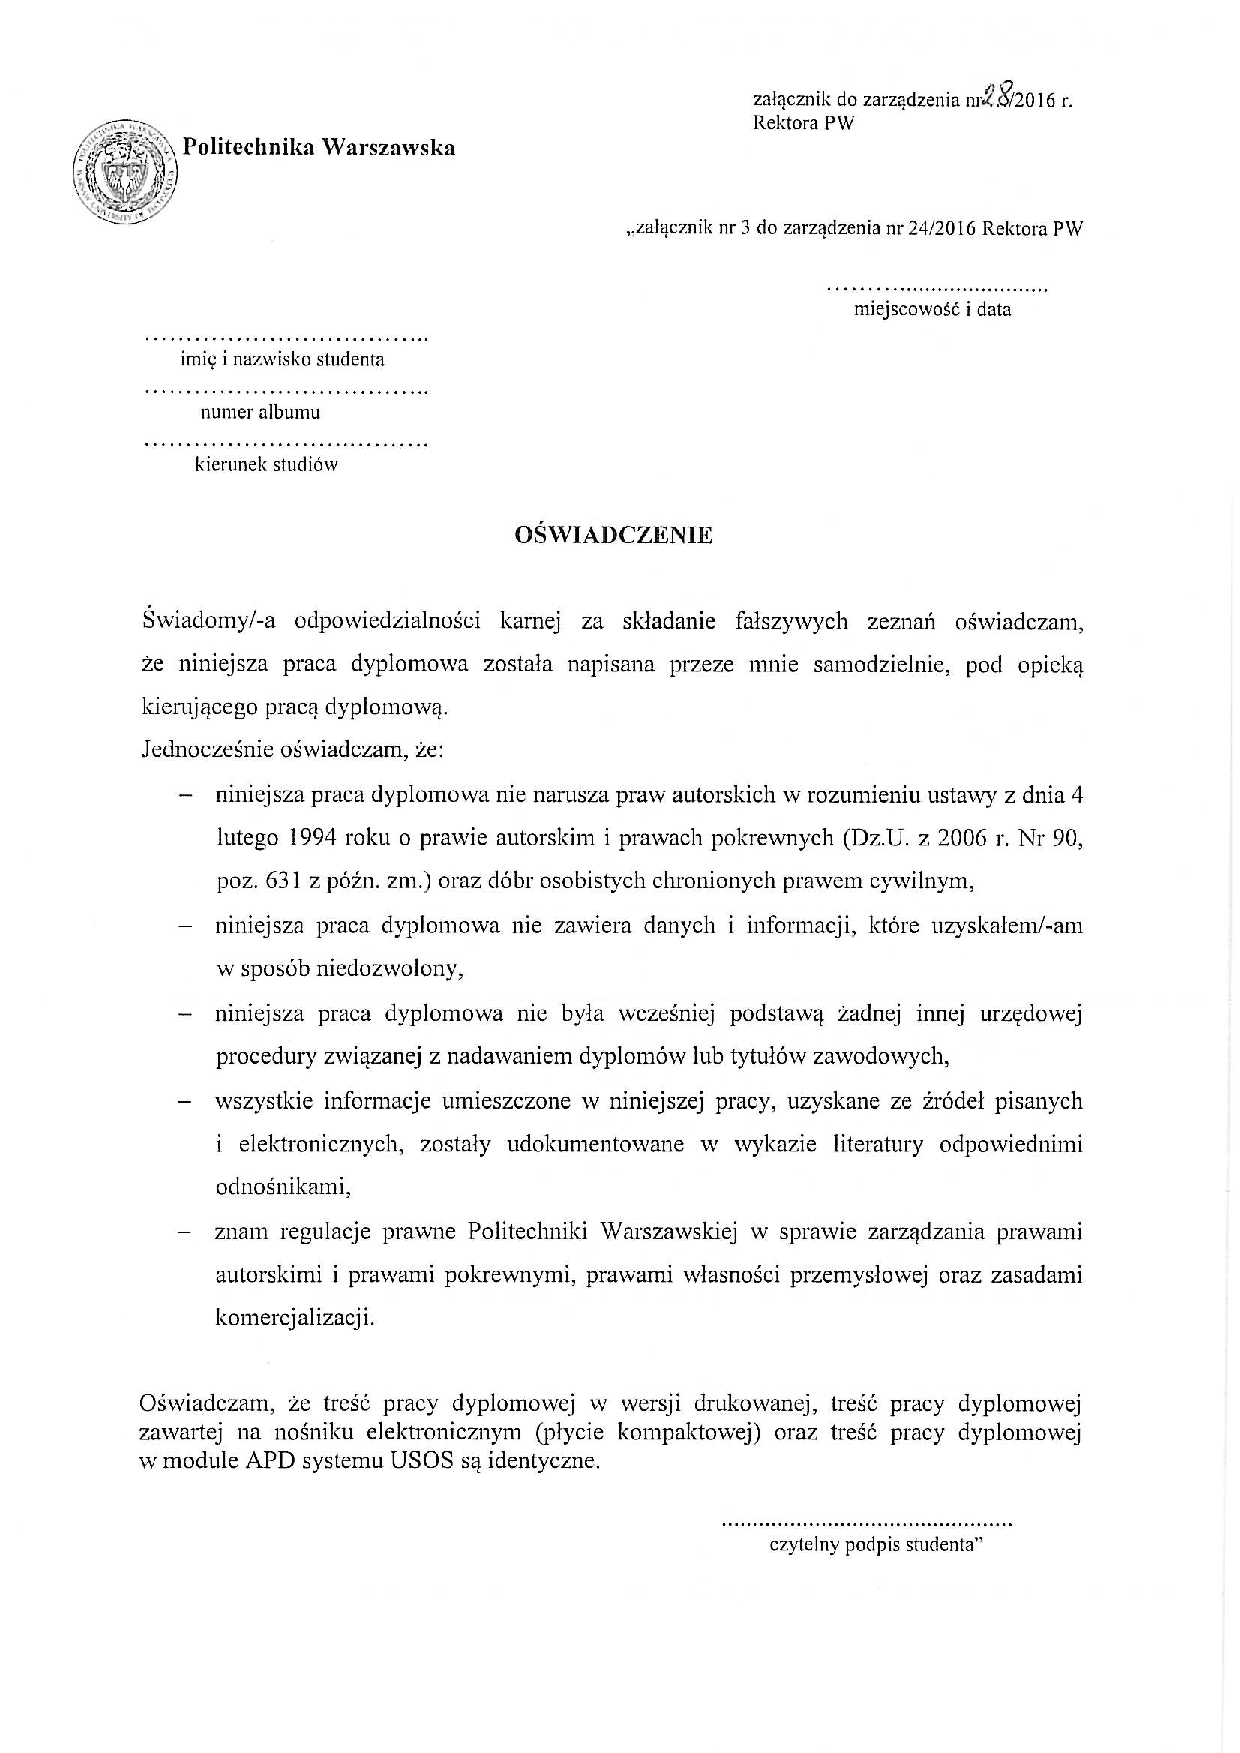
\includepdf[pagecommand={}]{pdf/oswiadczenie.pdf}
\clearpage\mbox{}\newpage


% PODZIĘKOWANIA




\clearpage

%\doublespacing
\tableofcontents
\onehalfspacing

% encoding: utf8
% !TEX encoding = utf8
% !TeX spellcheck = pl_PL

\chapter{Wstęp\label{chap:wstep}}

	Współczesne roboty z~powodzeniem zastępują człowieka przy wielu żmudnych i~niewdzięcznych czynnościach.  W~zakładach produkcyjnych sprawują się znakomicie, ale do współpracy robotów z~ludźmi podchodzi się niezwykle ostrożnie. Niechęć do tego typu działań podyktowana jest nie tylko wysokimi kosztami, ale także obawami związanymi z~ochroną otoczenia, w~którym robot ma operować.
	
	Zakres zastosowań robotyki można znacznie poszerzyć projektując roboty bezpieczne zarówno dla otaczającego je środowiska jak i~samych robotów. Jednym z~fundamentów takiego bezpieczeństwa może być algorytm sterowania impedancyjnego, który znacznie ogranicza ryzyko zniszczeń. 
	
	Prawo sterowania jest skonstruowane tak by silniki ramienia działały w~sposób symulujący układ ze sprężyną i~amortyzatorem. Robot sterowany w~taki sposób nie dąży do zadanej pozycji za wszelką cenę. W~momencie kolizji robot pozostaje elastyczny i~ugina się. Opisana zaleta może przerodzić się w~wadę. Algorytm korzysta ze zdefiniowanego modelu, który nie uwzględnia wszystkich cech ramienia oraz chwytanych przez robota przedmiotów. Z~punktu widzenia prawa sterowania chwycony przedmiot jest traktowany tak samo jak reszta środowiska. Zamiast skompensować siłę grawitacji tego przedmiotu ramię robota ugina się pod ciężarem. Dalsza manipulacja ramieniem najczęściej nie ma 
	sensu. 

	Celem pracy jest rozwiązanie problemu kompensacji siły grawitacji przedmiotu o~nieznanej masie i~inercji w~opisanym środowisku. 
	Do badań zostanie wykorzystany robot Velma oraz jego symulator skonstruowane przez Zespół Programowania Robotów i~Systemów Rozpoznających. W~niniejszej pracy zostanie zaprezentowana praktyczna realizacja sposobu kompensacji grawitacji chwyconego narzędzia wraz z~testami.

% encoding: utf8
% !TEX encoding = utf8
% !TeX spellcheck = pl_PL

\chapter{Podstawy teoretyczne\label{chap:przeglad_literatury}}
Dyskutowane w pracy algorytmy znane są w wielu różnych odmianach. Poniżej zaprezentowano wersje używane w trakcie dalszych badań. 

Do dalszych rozważań możemy zdefiniować uchyb jako:
\begin{equation}
	\boldsymbol{e_x} = \boldsymbol{x_d} - \boldsymbol{x}
\end{equation}
gdzie:
\begin{itemize}
\item $\boldsymbol{x_d}$ to wektor zadanych pozycji uogólnionych
\item $\boldsymbol{x}$ to wektor pozycji uogólnionych
\end{itemize}

\section{Sterowanie impedancyjne}
Prawo sterowania impedancyjnego w przestrzeni operacyjnej sprawia, że chwytak robota zachowuje się jak przytwierdzony do układu ze sprężyną i amortyzatorem. Pojawienie się nieprzewidzianych sił zewnętrznych powoduje, że uchyb pozycji nie jest minimalizowany za wszelką cenę. Przy kontakcie z otoczeniem stawy robota w pewnym stopniu sprężyste i miękkie. W konsekwencji robot ugina się przed otaczającym go środowiskiem. 

\subsection{Przypadek prosty}
W najprostszym przypadku możemy więc opisać takie prawo jako układ: 

	\begin{equation}
	F = kx + d\dot{x} + F_{ext}
	\end{equation}

gdzie:
\begin{itemize}
\item $F$ to siła wynikowa
\item $k$ to parametr sztywności
\item $d$ to parametr tłumienia
\item $F_{ext}$ to nieznana siła zewnętrzna działająca na układ
\end{itemize} 

\subsection{Prawo sterowania}
\label{sec:impedancyjne}

Można sformułować prawo sterowania jako wektor siły uogólnionej:
\begin{equation}
\boldsymbol{\mathcal{F}} = \boldsymbol{K_x}\boldsymbol{e_x} + \boldsymbol{D_x}\dot{\boldsymbol{e_x}}
\end{equation}

gdzie:
\begin{itemize}
\item $\boldsymbol{K_x}$ to diagonalna macierz sprężystości
\item $\boldsymbol{D_x}$ to diagonalna macierz tłumienia
\item $\boldsymbol{\mathcal{F}_{ext}}$ to wektor nieznanych uogólnionych sił zewnętrznych
\end{itemize}

\subsection{Sterowanie w przestrzeni konfiguracyjnej}
W rzeczywistym ramieniu robotycznym zadajemy momenty na poszczególne stawy robota. Opisane w podrozdziale \ref{sec:impedancyjne} prawo sterowania opisuje przestrzeń operacyjną $\boldsymbol{\mathcal{F}}$. Można uzyskać porządane wartości wektora momentów $\boldsymbol{\tau}$ które zadajemy silnikom w stawach stawie wyliczamy z jakobianu $\boldsymbol{J}$:

\begin{equation}
\boldsymbol{\tau} = \boldsymbol{J}^T(\boldsymbol{q})\boldsymbol{\mathcal{F}}
\end{equation}

\section{Sterowanie PID}
PID jest bardzo popularnym algorytmem sterowania automatycznego. Podstawowym celem algorytmu jest minimalizacja uchybu. Uchyb statyczny jest minimalizowany za wszelką cenę nawet jeśli miałoby to spowodować uszkodzenia. Uchyby dynamiczne nie są już tak dobrze kompensowane.

Człon proporcjonalny algorytmu pozwala na wzmocnienie uchybu i w ten sposób odjęcie go od sygnału sterującego. Człon całkujący algorytmu sumuje przeszłe błędy i odejmuje od sterowania ich sumę. Człon różniczkujący wzmacnia sygnał sterujący w gdy wartość błędu zmienia się w celu przyspieszenia regulacji.
\subsection{Przypadek prosty}
W jednowymiarowym przypadku prawo sterowania jest postaci:
\begin{equation}
F = Pe + I\int_{0}^{t}e dt + D\frac{de}{dt}
\end{equation}

gdzie:
\begin{itemize}
	\item $e$ to uchyb
	\item $P$ to parametr członu proporcjonalnego
	\item $I$ to parametr członu całkującego
	\item $D$ to parametr członu różniczkującego
\end{itemize}

\subsection{Przypadek wielowymiarowy}
Rozpatrując wektor siły uogólnionej możemy założyć że prawo sterowania rozpatruje każdą z wartości wektora niezależnie. Prawo sterowania można zapisać w postaci:
\begin{equation}
\boldsymbol{\mathcal{F}} = \boldsymbol{P}\boldsymbol{e_x} +\int_{0}^{t}  \boldsymbol{I}\boldsymbol{e_x}dt + \boldsymbol{D}\dot{\boldsymbol{e_x}}
\end{equation}
gdzie:
\begin{itemize}
	\item $\boldsymbol{P_x}$ to diagonalna macierz proporcjonalności
	\item $\boldsymbol{I_x}$ to diagonalna macierz członu całkowania
	\item $\boldsymbol{D_x}$ to diagonalna macierz członu różniczkującego
\end{itemize}

\section{Estymacja siły uogólnionej w końcówce}
Dla ramienia robotycznego możemy opisać siły występujące w samym ramieniu zgodnie ze wzorem:
\begin{equation}
\boldsymbol{\mathcal{F}_m}(\boldsymbol{x}, \dot{\boldsymbol{x}}, \ddot{\boldsymbol{x}}, \boldsymbol{q}, \dot{\boldsymbol{q}}) = \boldsymbol{\Lambda}(\boldsymbol{q})\boldsymbol{\ddot{x}} + \boldsymbol{\mu}(\boldsymbol{x}, \boldsymbol{\dot{x}}) + \boldsymbol{\gamma}(\boldsymbol{q}) + \boldsymbol{\eta}(\boldsymbol{q}, \boldsymbol{\dot{q}}) + \boldsymbol{\mathcal{F}_{ext}}
\label{eq:ramie}
\end{equation}

gdzie:
\begin{itemize}
	\item $\boldsymbol{\mathcal{F}}$ to wektor sił wynikowych
	\item $\boldsymbol{\Lambda}$ to dodatnio określona macierz inercji w przestrzeni zadań
	\item $\boldsymbol{\mu}$ to macierz sił Coriolisa i sił odśrodkowych	
	\item $\boldsymbol{\gamma}$ to wektor sił grawitacji
	\item $\boldsymbol{\eta}$ to macierz sił tarcia oraz nieuwzglęnionych sił
	\item $\boldsymbol{q}$ to wektor położeń stawów w przestrzeni konfiguracyjnej
	\item $\boldsymbol{x}$ to wektor położeń końcówki w przestrzeni zadań
	\item $ \boldsymbol{\mathcal{F}_{ext}}$ to nieznany wektor sił zewnętrznych działających na układ
\end{itemize} 

Przy wyliczaniu estymowaniu sił działających na końcówkę należy pamiętać, że w końcówce występują siły wygenerowane przez prawo sterowania oraz rzeczywiste siły występujące w układzie. Wzór estymujący rzeczywistą wartość siły uogólnionej w końcówce można zapisać jako:
\begin{equation}
\boldsymbol{\mathcal{\hat{F}}} = \boldsymbol{\mathcal{F}} + \boldsymbol{\mathcal{F}_m}(\boldsymbol{x}, \dot{\boldsymbol{x}}, \ddot{\boldsymbol{x}}, \boldsymbol{q}, \dot{\boldsymbol{q}})
\end{equation}

gdzie $\boldsymbol{\mathcal{F}}$ to wektor sił uogólnionych wyliczony prawem sterowania.

QUESTION: czy rozwijac ta mysl skoro teog nie implementuje?

\section{Ocena jakości algorytmów sterowania}
\subsection{Jakość sterowania}
Prostym sposobem oceny jakości algorytmu sterowania jest konfrontacja rzeczywistych pozycji ramienia robota z zadanymi. W pracy przyjęto metrykę APE (ang. Absolute Trajectory Error). Metryka jest popularnym wskaźnikiem testowania algorytmów SLAM (ang. Simultaneous Localization and Mapping) ale może być też użyta do porównania trajektorii zadanej przez interpolator i rzeczywistej. 

Dwie trajektorie są opisane w postaci list wektorów sił uogólnionych $\boldsymbol{P}_{1..n}$ oraz $\boldsymbol{Q}_{1..n}$ gdzie $n$ to ilość próbek. Dla każdej chwili czasowej $i$ jest wyliczany błąd postaci:
\begin{equation}
\boldsymbol{E}_i = \boldsymbol{Q}_i^{-1}\boldsymbol{S}\boldsymbol{P}_i
\end{equation}
Macierz $\boldsymbol{S}$ jest optymalnym w sensie metody najmniejszych kwadratów rzutowaniem wektora $\boldsymbol{Q}_i$ na wektor $\boldsymbol{P}_i$ znalezionym za pomocą metody Horna TODO: cyowania. 

Błąd całkowity jest wyliczany jako błąd średniokwadratowy:
\begin{equation}
RMSE(\boldsymbol{E}_{1..n}) = \sqrt{\frac{1}{n}\sum_{i=1}^{n}||\boldsymbol{E}_i||^2}
\end{equation}.

\subsection{Jakość kontaktu z otoczeniem }
Największą zaletą sterowania impendancyjnego jest ugięcie ramienia robota w momencie kolizji ze środowiskiem. Ocena jakości tej cechy może być opisana jako odchylenie pozycji stawów $\boldsymbol{q}_i$ w stosunku do ustalonej pozycji sprzed kolizji $\boldsymbol{q}$ w chwili $i$.


Błąd całkowity jest wyliczany jako błąd średniokwadratowy:
\begin{equation}
RMSE(\boldsymbol{R}_{1..n}) = \sqrt{\frac{1}{n}\sum_{i=1}^{n}||\boldsymbol{q_d}-\boldsymbol{q}_i||^2}
\end{equation}.

\section{Teoria agenta upostaciowionego}
Agentem możemy nazwać jednostkę która jest: zdolna do komunikowania się ze środowiskiem, zdolna do monitorowania swego otoczenia i podejmowania autonomicznych decyzji. Taka definicja gwarantuje spełnienie wielu cech których oczekujemy od nowoczesnych systemów robotycznych. Z definicji agenty są w stanie samodzielnie reagować na zmiany zachodzące w środowisku w sposób inteligentny. Rozszerzeniem teorii agentowej jest teoria agenta upostaciowionego. Agent upostaciowiony cechuje się tym czym zwykły agnet oraz posiada fizyczne ciało.


W teorii agenta upostaciowionego występują pojęcia rzeczywistych efektorów i receptorów. Służą one odpowiednio do oddziaływania na środowisko i do pozyskiwania wiedzy o tym środowisku. W praktyce oznacza to, że rzeczywistym efektorem może być silnik a rzeczywistym receptorem enkoder. 

Agent $a$ może się składać z trzech podsytemów:
\begin{itemize}
	\item Podsystemu sterowania $c$ który zajmuje się podejmowaniem decyzji na podstawie danych z innych podsystemów. Agent może mieć tylko jeden podsystem sterowania.
	\item Wirtualnego efektora $e$ który pośredniczy w komunikacji pomiędzy podsystemem sterowania i rzeczywistym efektorem.
	\item Wirtualnego receptora $r$ który pośredniczy w komunikacji pomiędzy podsystemem sterowania i rzeczywistym receptorem.
\end{itemize}
Podsystemy składają się z komponentów czyli algorytmów. Każdy z podystemów może mieć wiele komponentów i nie wszystkie muszą być uruchomione w konkretnej chwili. Agent posiada też zdefiniowaną maszynę stanów które mogą się zmieniać przy pomocy funkcji przejścia (predykatów). Stan maszyny stanów definiuje tak zwane zachowanie agenta czyli sposób reakcji podsystemu sterowania i uruchomione komponenty. Dodatkowo agent ma możliwość wymiany danych innymi agentami oraz rzeczywistymi efektorami i receptorami poprzez bufory transmisyjne $T$. 
% encoding: utf8
% !TEX encoding = utf8
% !TeX spellcheck = pl_PL

\chapter{Środowisko badawcze\label{chap:srodowisko}}
	\section{Budowa ogólna}
	Środowiskiem badawczym jest robot usługowy Velma. Został zaprojektowany i wykonany przez Zespół Rrogramowania Robotów i Systemów Rozpoznających. Do obrotowego korpusu przytwierdzono dwa ramiona robotyczne Kuka LWR-4+. Mają siedem stopni swobody i udzwig 7 kg. Na ich końcach znajdują się chwytaki Barretta oraz nadgarstkowe czujniki FTS. Głowa robota umieszczona jest na dedykowanej konstrukcji która za pomocą dwóch silników elektrycznych pozwala na zginianie i obrót głowy. Robot wyposażony jest w czujnik wizyjny Microsoft Kinect oraz dwie kamery połączone w stereoparę. Do głowy zamocowano mikrofon. Ramiona robota są połączone z komputerem sterującym przy pomocy magistral FRI a pozostałe przy pomocy magistrali EtherCAT. 
	
	System sterowania o twardych ograniczeniach czasowych pracuje z częstotliwością 500 Hz. Struktura oprogramowania została stworzona w oparciu o teorię agentową. Oprogramowanie robota pisane jest przy wykorzystaniu struktury ramowej FABRIC. Programy nadzoruje system Linux z nakładką Linux-RT. Dostępny jest symulator robota stworzony w przy wykorzystaniu Gazebo i silnika fizyki DART. 
	

	\section{Pakiety oprogramowania}
	\subsection{ROS}
	Struktura ramowa ROS (Robot Operating System)\cite{bib:ROS} zapewnia biblioteki usprawniające pisanie programów dla robotyki w C++ i Pythonie. Pozwala na komunikację pomiędzy programami na zasadzie tematów oraz na zasadzie usług. Posiada gotowe funkcje liczące kinematykę i wizualizujące pracę robota. Daje możliwość akwizycji danych. Podstawowymi narzędziami w pakiecie są:
	\begin{itemize}
		\item \textbf{Węzły} - Programy pisane w C++ lub Pythonie spełniające zdefiniowaną w sytemie funkcję.
		\item \textbf{Serwisy} - Usługi udostępniane przez węzły pozwalające na komunikację w architekturze zapytanie odpowiedź. Każdy program może udostępniać wiele serwisów. Służą do wywoływania zdalnych procedur.
		\item \textbf{Akcje} - Usługi podobne do serwisów lecz nieblokujące wykonywania węzła będącego serwerem.
		\item \textbf{Tematy} - Usługi udostępniane przez węzły pozwalające na asynchroniczną komunikację. Każdy program może udostępniać i pobierać wiele tematów. Służą do aktualizowania bierzącego stanu całego systemu.
		\item \textbf{Zarządca} - odpowiada za komunikację i nadzoruje pracę innych narzędzi pakietu.
	\end{itemize}
	\subsection{Orocos}
	Orocos jest wolnym oprogramowaniem napisanym w C++ służącym do pisania aplikacji zgodnych z wymaganiami czasu rzeczywistego. Pozwala na tworzenie komponentów odwzorowujących modele stworzone przy pomocy teorii agentowej. Zestaw bibliotek składa się między innymi z:
	\begin{itemize}
		\item \textbf{RTL (ang. Real-Time Toolkit)} - Biblioteki służące do  tworzenia komponentów w aplikacjach czasu rzeczywistego.
		\item \textbf{OCL (ang. Orocos Component Library)} - Biblioteki pomocne w trakcie uruchamiania komponentów.
		\item \textbf{OroGen} oraz \textbf{TypeGen} - Narzędzia do automatycznego generowania komponetów i typów danych.
		\item \textbf{Deployer} - Uruchamia komponenty zgodnie z opisem zawartym w pliku XML oraz pozwala na nadzór tych komponentów trakcie pracy.
	\end{itemize}

	\subsection{FABRIC}
	Framework for Agent–Based Robot Control Systems - FABRIC\cite{Seredynski-fabric-romoco-2019-twiki} wykorzystuje Orocosa oraz strukturę ramową ROS zapewniając interfejs programistyczny pozwalający na tworzenie komponentów zgodnych z założeniami teorii agentowej. Ma zaimplementowane algorytmy komunikacji pomiędzy poszczególnymi podsystemami poprzez zdefiniowane wiadomości. Posiada narzędzie wizualizujące stan predykatów, zachowań i podsystemów \textit{rqt\_agent}. Pokazuje też przepływ danych między komponentami.

	
	\section{Symulator robota}
	Symulator robota Velma jest wytworzony w oprogramowaniu Gazebo które symuluje obiekty i zachowania między nimi zgodnie z prawami fizyki. Użytkownik ma możliwość zdefiniowania całego środowiska wraz z robotem. Posiada gotowe modele wielu receptorów i efektorów oraz daje możliwość tworzenia własnych. Daje możliwość emulowania sterowników sprzętu. Pozwala na wywarcie siły bądź momentu na dowolny przedmiot będący w symulacji. Emuluje czas jeśli symulacja nie jest przeprowadzana w czasie rzeczywistym.

	Orginalny kod Gazebo został zmodyfikowany przez Zespół programowania Robotów i Systemów Rozpoznających aby można było korzystać z pakietu oprogramowania DART (ang. Dynamic Animation and Robotics Toolkit) symulującego fizykę zdefiniowanego świata. Pakiet DART został wybrany przez Zespół programowania Robotów i Systemów Rozpoznających ponieważ po jego zastosowaniu został wyeliminowany problem narastających oscylacji członów robota w trakcie symulacji. W przeciwieństwie do wielu symulatorów fizyki daje dostęp do wielu przydatnych informacji takich jak jakobian bądź macierz inercji przemiotów. Zastosowanow w nim algorytm LPC (ang. Linear complementarity problem) który sprowadza model fizyczny świata do zestawu równań kwadratowych. DART symuluje działanie wielu sił w tym Coriolisa i tarcia dynamicznego. Dzięki temu możliwe jest zaawansowane wykrywanie kolizji. 
	
	\section{Agenty}
	System sterowania zbudowany jest z dwóch agentów. Agent \textit{velma\_core} jest odpowiedzialny za kontrolę zadań związanych z manipulacją w przestrzeni operacyjnej i konfiguracyjnej robota. Drugi z agentów \textit{velma\_task\_cs\_ros\_interface} jest interfejsem pomiędzy programami użytkownika pisanymi w ROS oraz agentem \textit{velma\_core}. Zawiera tylko jeden podsystem o tej samej nazwie.

	Podsystem \textit{velma\_core\_cs} agenta \textit{velma\_core} wylicza prawa sterowanie oraz zajmuje się interpolacją trajektorii. Podsytem \textit{velma\_core\_ve\_body} kontroluje bazowe zachowania bezpieczeństwa. Są to ograniczenia prądowe, wykrywanie krańcowych położeń stawów oraz wykrywanie kolizji. Podsystem przekazuje też sterowanie do efektorów. Podsystemy w najniższej warstwie abstrakcji mogą być stosowane wymiennie. Do pracy w rzeczywistym świecie uruchamiane są podsystemy \textit{velma\_core\_re\_lwr\_r} i \textit{velma\_core\_re\_lwr\_l} oraz podsystem \textit{velma\_ec\_driver}. Służą odpowiednio do kontroli prawego i lewego ramienia LWR-4 oraz pozostałego sprzętu połączonego magistralą EtherCAT. Do pracy w trybie symulacji podsystemy w najniższej warstwie abstrakcji są wymieniane na podsystem \textit{velma\_sim\_gazebo} w którym uruchamiany jest symulator świata Gazebo. Podsystem symuluje pracę wszystkich trzech podsystemów odpowiedzialnych za komunikację ze sterownikami sprzętu. 


	\begin{itemize}
	\item \textbf{Interfejs akcji ROS} - 
	Komponent \textit{CartImpActionRight} znajduje się w podsytemie \textit{velma\_task\_cs\_ros\_interface} i odbiera rozkazy wysłane przez użytkownika przez mechanizm akcji ROS oraz przesyła je do innych podsytemów. Zwraca też status wykonania operacji. Komponent służy do obsługi prawego ramienia i istnieje analogiczny komponent \textit{CartImpActionLeft} służący do obsługi lewego ramienia.
	\item \textbf{Publikacja wektorów pozycji} - 
	Komponent \textit{TfPublisher} wysyła do użytkownika za pomocą ROSa położenie i obrót istotnych dla działania systemu miejsc robota takich jak chwytaki czy środek cięzkości korpusu. 
	\item \textbf{Pozycje stawów} - 
	Odczyt pozycji stawów jest zależny od trybu pracy oprogramowania. Jeśli używamy trybu obsługi rzeczywistego sprzętu to za odczyt pozycji są odpowiedzialne podsystemy \textit{velma\_core\_re\_lwr\_r} i \textit{velma\_core\_re\_lwr\_l} oraz podsystem \textit{velma\_ec\_driver} które posiadają pojedyncze komponenty służące do komunikacji z fizycznymi sterownikami magistral. W trybie symulatora emulacją tych trzech podsystemów zajmuje się podsytem \textit{velma\_sim\_gazebo} który jako symulator nie jest podzielony na konkretne podsystemy.
	\item \textbf{Zadawanie momentów} - 
	Zadawanie momentów obrotowych w stawach następuje w analogiczny do odczytywania pozycji sposób.
	\item \textbf{Kinematyka prosta} - 
	Komponent \textit{FK} pobiera dane o pozycjach stawów i wylicza pozycję chwytaka oraz innych części robota.
	\item \textbf{Interpolator trajektorii} - 
	Komponent \textit{INT\_tool\_r} z podsystemu \textit{velma\_core\_cs} odpowiada za interpolacje trajektorii zadanej prawemu ramieniu. Interpolator służy temu by jedno polecenie przesunięcia ramienia zamienić na wiele mniejszych i rozłożonych w czasie. W konsekwencji algorytm sterowania nie jest narażony na duże uchyby a ruch ramienia jest wykonywany płynnie. Do działania komponent potrzebuje aktualnych i zadanych pozycji. Komponent służy do obsługi prawego ramienia. Analogicznie do obsługi lewego ramienia służy komponent \textit{INT\_tool\_l}.

	\item \textbf{Prawo sterowania impedancyjnego} - 
	Komponent \textit{cart\_imp} z podsytemu \textit{velma\_core\_cs} służy do wyliczania momentów zadawanych na stawy zgodnie z algorytmem prawa sterowania impedancyjnego w przestrzeni kartezjańskiej. Pobiera zadaną pozycję z interpolatora trajektorii.
	\end{itemize}
% encoding: utf8
% !TEX encoding = utf8
% !TeX spellcheck = pl_PL

\chapter{Specyfikacja systemu \label{chap:specyfikacja_systemu}}
Sterowanie impedancyjne w przestrzeni operacyjnej zastosowane w robocie Velma kompensuje jedynie masę członów własnych. Gdy manipulator chwyci narzędzie powstaje znaczny uchyb, który nie jest kompensowany. W przypadku chwycenia przedmiotu o dużej masie ramię robota jest wręcz unieruchomione. Należy skonstruować i zaimplementować algorytm kompensacji siły grawitacji narzędzia o nieznanych parametrach. 

\section{Wymagania}
Wymagania są narzucone przez system środowiska badawczego.
\begin{itemize}
	\item Do działania systemu wymagane jest ramię robotyczne sterowane prawem sterowania impedancyjnego w przestrzeni kartezjańskiej
	\item System dostarcza gotowe komponenty potrzebne do pracy ramienia, w szczególności: generatora trajektorii, interpolatora oraz wyznaczania kinematyki prostej 
	\item System pozyskuje dane o otoczeniu na podstawie odczytów z czujników położenia stawów.
	\item System samodzielnie kompensuje siłę grawitacji związaną z masą wszystkich członów robota
	\item Parametry chwytanego obiektu związane z masą i inercją nie są znane i mogą być zmienne w czasie
\end{itemize}

\section{Założenia}
Algorytm kompensacji grawitacji musi wyliczać dodatkowy moment w stawach robota. Do momentów obrotowych wyliczanych na postawie  prawa sterowania impendancyjnego w przestrzeni operacyjnej robota należy dodać te związane z kompensacją masy narzędzia.
\begin{itemize}
	\item Wyliczone przez prawo sterowania momenty zadawane w stawach zostaną zmodyfikowane przez algorytm kompensacji grawitacji
	\item Algorytm kompensacji ma minimalizować uchyb statyczny wynikający z chwycenia przedmiotu o nieznanej masie i inercji.
	\item  Trajektoria końcówki ramienia powinna być zbliżona do trajektorii analogicznego ruchu bez uchwyconego przedmiotu.
	\item Algorytm kompensacji nie może zaburzać cech sterowania imedancyjnego pozwalających na uginanie się robota w momencie kolizji
\end{itemize}


\section{Przypadki użycia}
Przypadki użycia (rys. \ref{fig:usecase}) odzwierciedlają pracę systemu po modyfikacji. Algorytm kompensujący ma działać przez cały czas pracy robota gdy pracuje z narzędziem. Przypadki użycia są zbieżne z przypadkami użycia robota kiedy pracuje w trybie sterowania impedancyjnego.

\begin{figure}[H]
	\centering
	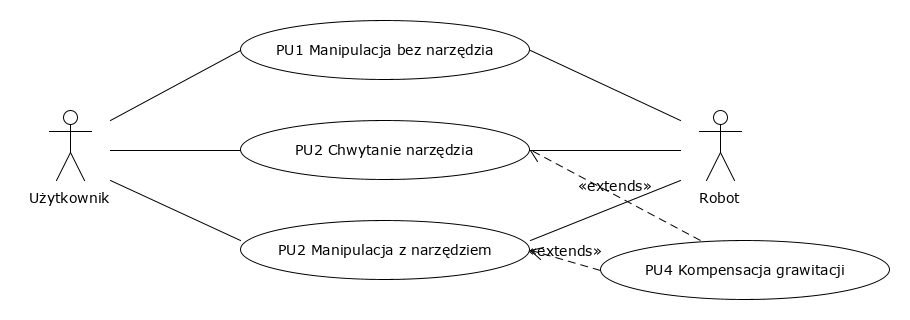
\includegraphics[width=.9\textwidth]{images/usecase.png}
	\caption{Diagram przypadków użycia robota z uwzględnieniem algorytmu kompensacji grawitacji}
	\label{fig:usecase}
\end{figure}


Aktorami korzystającymi z systemu są:
\begin{itemize}
	\item \textbf{Robot} - robot wykonujący zadanie chwycenia obiektu
	\item \textbf{Użytkownik} - system zewnętrzny wydający polecenia
\end{itemize}


Można wyszczególnić następujące przypadki użycia:
\begin{itemize}
	\item \textbf{PU1 Manipulacja bez narzędzia} - Konfiguracja ramienia robota może się zmieniać lecz robot nie trzyma żadnego narzędzia. Algorytm kompensacji grawitacji nie powinien zmieniać prawa sterowania. 
	\item \textbf{PU2 Chwytanie narzędzia} - Robot zaciska chwytak na narzędziu o nieznanych parametrach a następnie je podnosi.  
	\item \textbf{PU3 Manipulacja z narzędziem} - Konfiguracja ramienia może się zmieniać a algorytm kompensacji grawitacji powinien przeciwdziałać sile grawitacji chwyconego narzędzia.
	\item \textbf{PU4 Kompensacja grawitacji} - Robot kompensuje siłę grawitacji chwyconego narzędzia
\end{itemize}




% encoding: utf8
% !TEX encoding = utf8
% !TeX spellcheck = pl_PL

\chapter{Implementacja systemu\label{chap:implementacja_systemu}}
W ramach pracy zmodyfikowano istniejący system robotyczny opisany w rozdziale \ref{chap:srodowisko}. Dzięki temu możliwe było spełnienie założeń i wymagań z rozdziału \ref{chap:specyfikacja_systemu}. 


\section{Kompensowanie wpływu grawitacji narzędzia}
Kiedy chwytak robota chwyci narzędzie zmienia się łańcuch kinematyczny. W pracy zajmujemy się przypadkiem w którym po uchwyceniu narzędzie zostaje nieruchome w stosunku do chwytaka. Można przyjąć, że zmieniają się wtedy parametry ostatniego członu związane z masą i inercją.

Głównym problemem w trakcie manipulacji z nieskompensowaną grawitacją jest znaczny uchyb statyczny. Aby wyeliminować ten efekt można do istniejącego algorytmu sterowania impedancyjnego dodać algorytm PID. 

Należy mieć na uwadze, że niektóre człony są takie same w zaprezentowanych prawach sterowania. W impedancyjnym prawie sterwowania nie ma członu całkującego i został on skopiowany z algorytmu PID. W rezultacie nowe prawo sterowania jest postaci:

\begin{equation}
\boldsymbol{\mathcal{F}} = \boldsymbol{K_x}\boldsymbol{e_x} + \boldsymbol{D_x}\dot{\boldsymbol{e_x}} + \int_{0}^{t}  \boldsymbol{I}\boldsymbol{e_x}dt
\end{equation}

gdzie:
\begin{itemize}
    \item $\boldsymbol{\mathcal{F}}$ to wektor sił wynikowych
    \item $\boldsymbol{K_x}$ to diagonalna macierz sprężystości
    \item $\boldsymbol{D_x}$ to diagonalna macierz sztywności
    \item $\boldsymbol{I}$ to diagonalna macierz członu całkującego
    \item $\boldsymbol{e_x}$ to wektor uchybu
\end{itemize}
% encoding: utf8
% !TEX encoding = utf8
% !TeX spellcheck = pl_PL

\chapter{Działanie systemu\label{chap:weryfikacja_systemu}}
\graphicspath{{../../velma/przerobione_testy/out/}{./images}}

Algorytm kompensacji grawitacji zaimplementowano modyfikujac komponent \textit{cart\_imp} odpowiedzialny za wyliczanie prawa sterowania oraz inne komponenty. W celu weryfikacji wymagań systemu zostal napisany program komunikujacy sie z agentem \textit{velma\_ros\_interface}. Program  nakazujacy robotowi manipulowanie chwytakiem w trybie sterowania impedancyjnego w przestrzeni operacyjnej uruchomiono w trybie symulacji. Program jest uruchamiany w trybie wysokiej i niskiej sprezystosci oraz z wlaczonym i wylaczonym algorytmem kompensacji grawitacji. W trakcie wszystkich eksperymentow wszystkie parametry algorytmu sterowania byly takie same. TODO: dodac osie w sekcji o robocie 

\section{Ocena jakosci sterowania}
Okreslenie jakosci algorytmu mozliwe jest dzieki modyfikacji komponentu \textit{TfPublisher}. Po modyfikacji udostepnia on dane o pozycji zadanej z interpolatora trajektorii oraz o pozycji osiagnietej. Ocena jakosci sterowania nastepuje poprzez porownanie wynikow obliczonych zgodnie z metryka APE opisanej w sekcji \ref{chap:ape}. W pracy nie zamieszczono wynikow dzialania algorytmu sterowania bez kompensacji i z chwyconymi przedmiotami poniewaz nie byly one w zadnym stopniu wykonywane. Testy polegaly na chwytaniu dwoch przedmiotow. Puszka ma wage ok 1 kg jest walcem z rowomiernie rozlozona masa. Wiertarka ma wage ok 1,5 kg i jej rozklad mas nie jest rownomierny.


\subsection{Ruch ósemkowy}

Eksperyment ma przetestowac zachowanie algorytmu kompensacji przy skomplikowanych ruchach (rys. \ref{fig:osemka_a}, \ref{fig:osemka_rot}).  Ruch "osemkowy" zadany jest w osi $Y$ oraz $Z$.
Trajektoria jest zadana zgodnie ze wzorem lemniskaty Bernoulliego opisanej wzorem:
\begin{equation}
(y^2 + z^2)^2 = 2a^2(y^2-z^2)
\end{equation}

gdzie:
\begin{itemize}
	\item $y$ oraz $z$ to wspolrzedne trajektorii
	\item $a$ to parametr rownania
\end{itemize}

Trajektoria ruchu w rzucie na wprost ruchu zostala zaprezentowana na rys. \ref{fig:osemka_porow_komp}, \ref{fig:osemka_porow_przedm} i \ref{fig:osemka_porow_zbiorcze_a}. Trajektoria widoczna z boku (w osiach $X$ oraz $Z$) zostala zaprezentowana na rys. \ref{fig:osemka_porow_komp_bok}, \ref{fig:osemka_porow_przedm_bok} i \ref{fig:osemka_porow_zbiorcze_b}.
\begin{figure}[h]
	\centering
	\subfigure[Os $X$]{
		\label{fig:osemka_ax}
		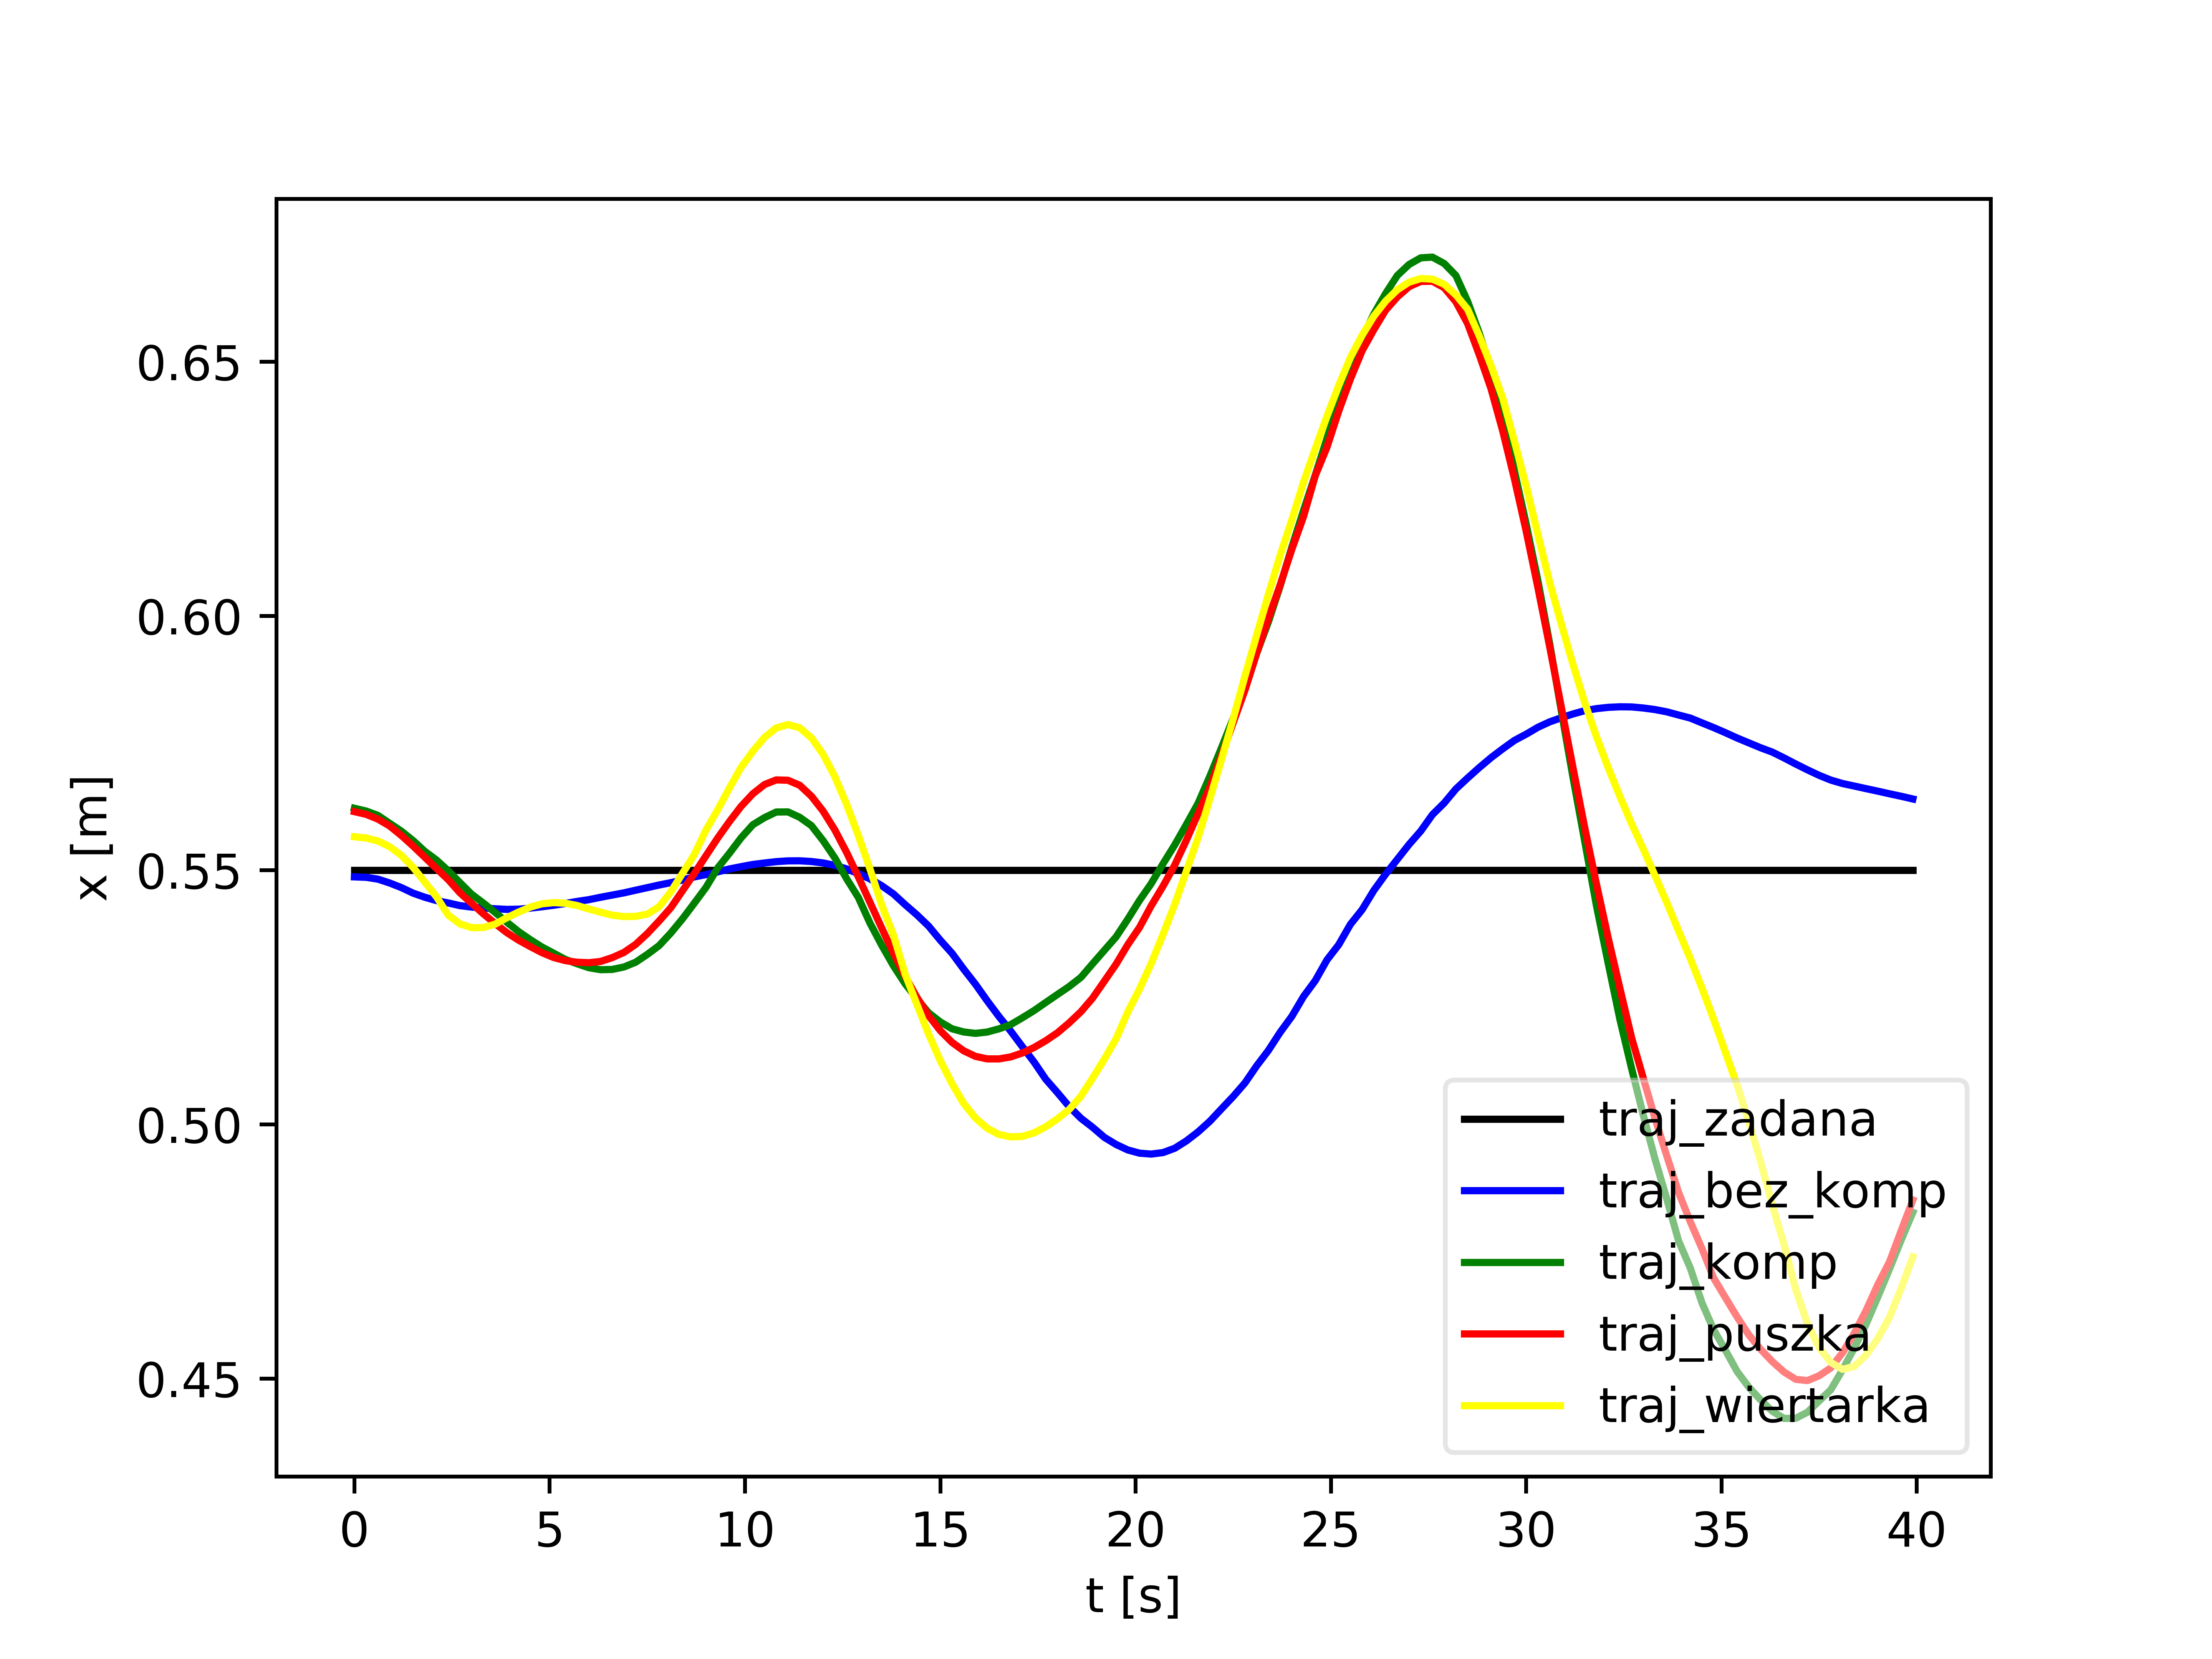
\includegraphics[width=.45\textwidth]{../../velma/przerobione_testy/out/osemka/common_ax.png}
	}
	\hfill
	\subfigure[Os $Y$]{
		\label{fig:osemka_ay}
		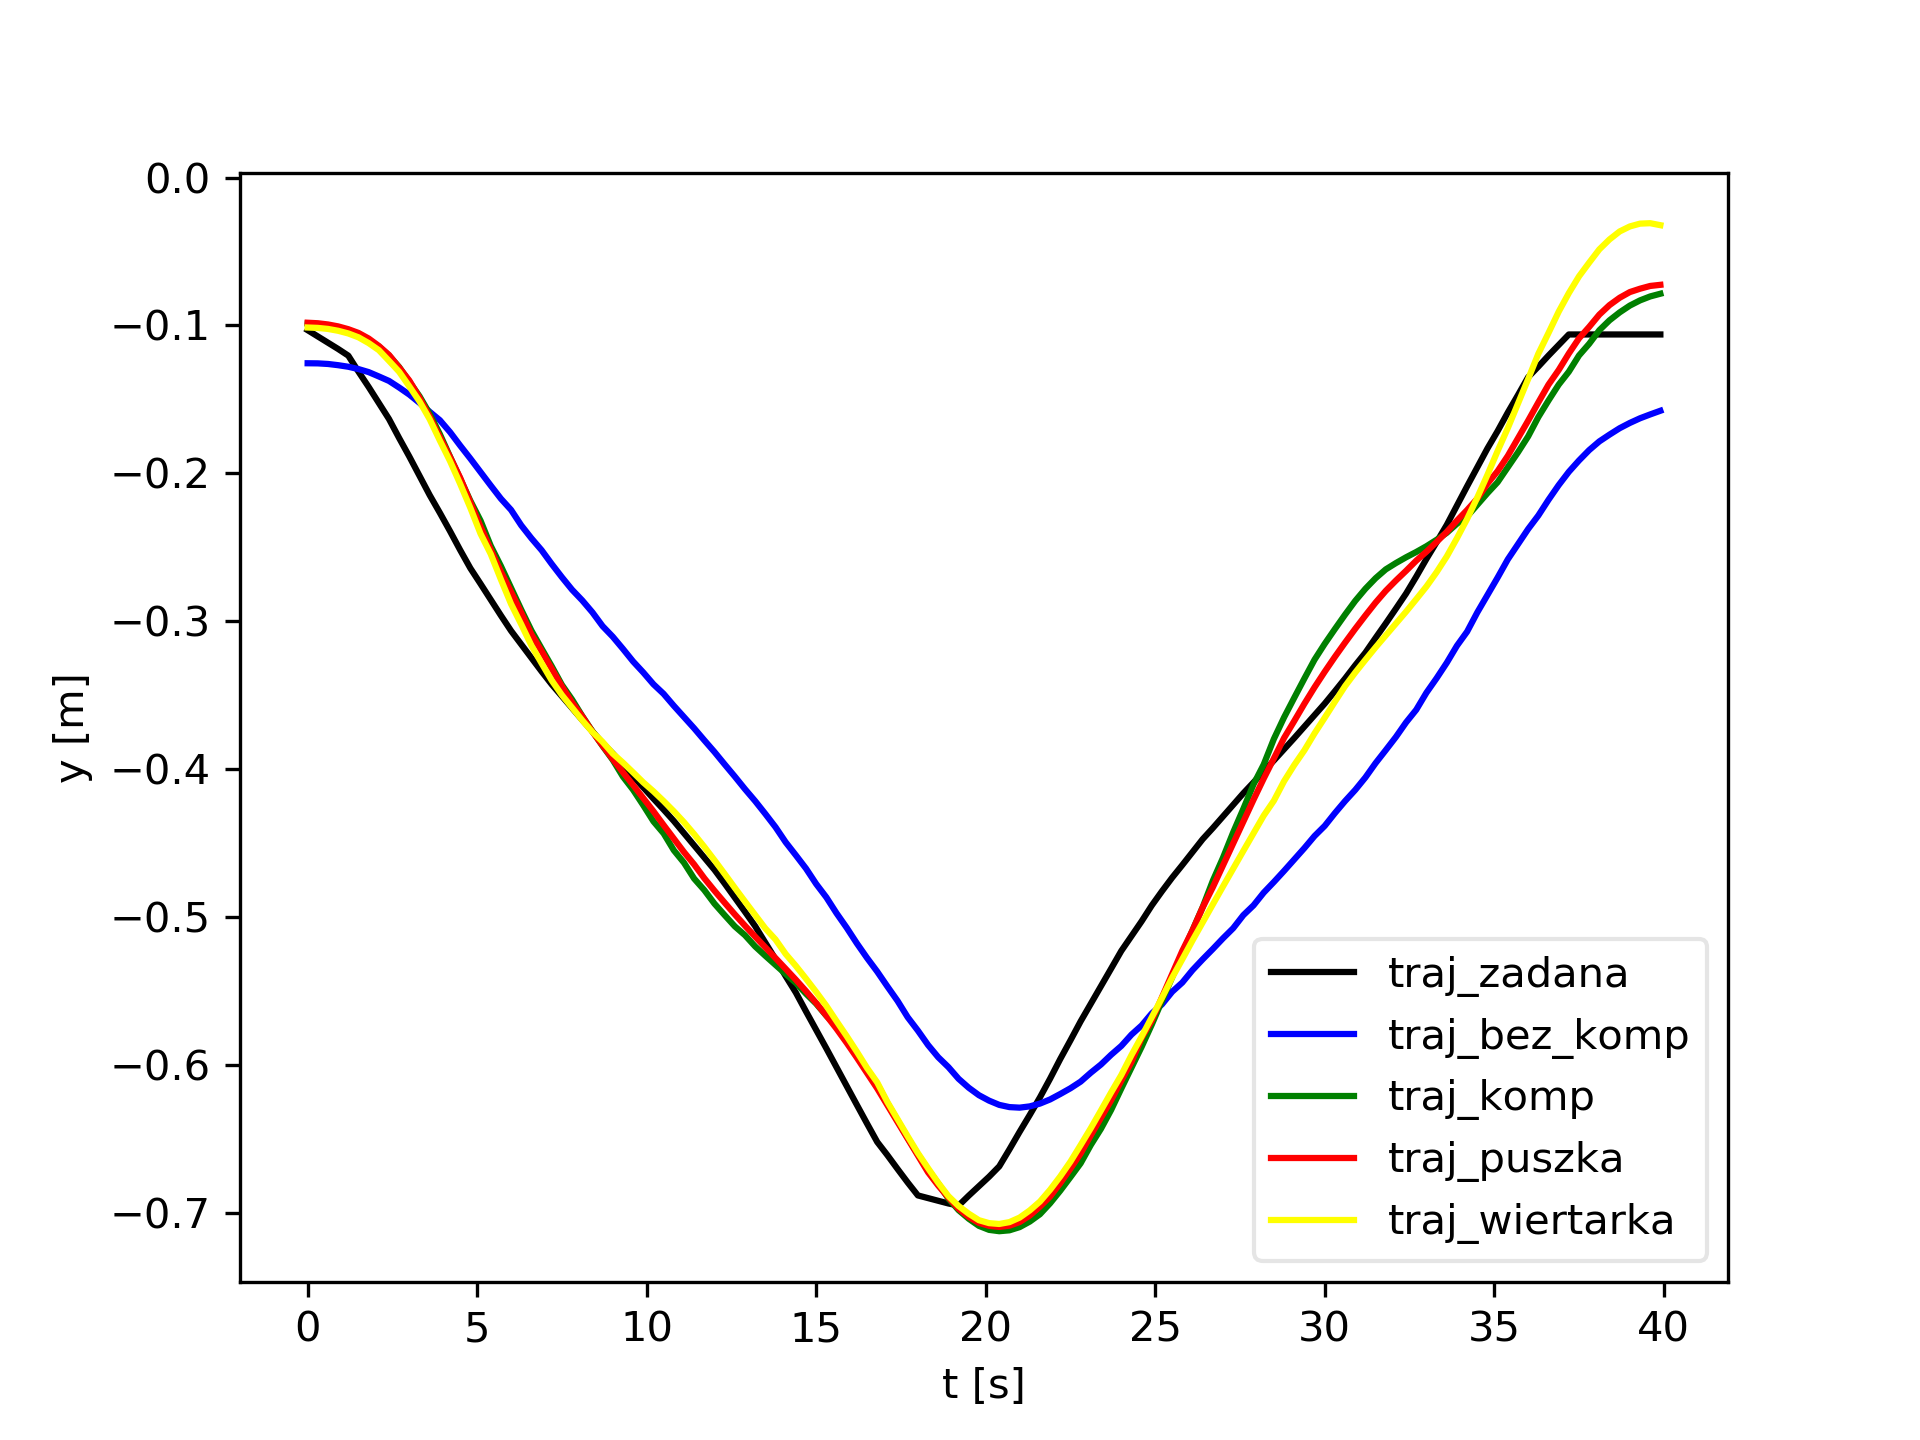
\includegraphics[width=.45\textwidth]{../../velma/przerobione_testy/out/osemka/common_ay.png}
	}
	
	\hfill
	\subfigure[Os $Z$]{
		\label{fig:osemka_az}
		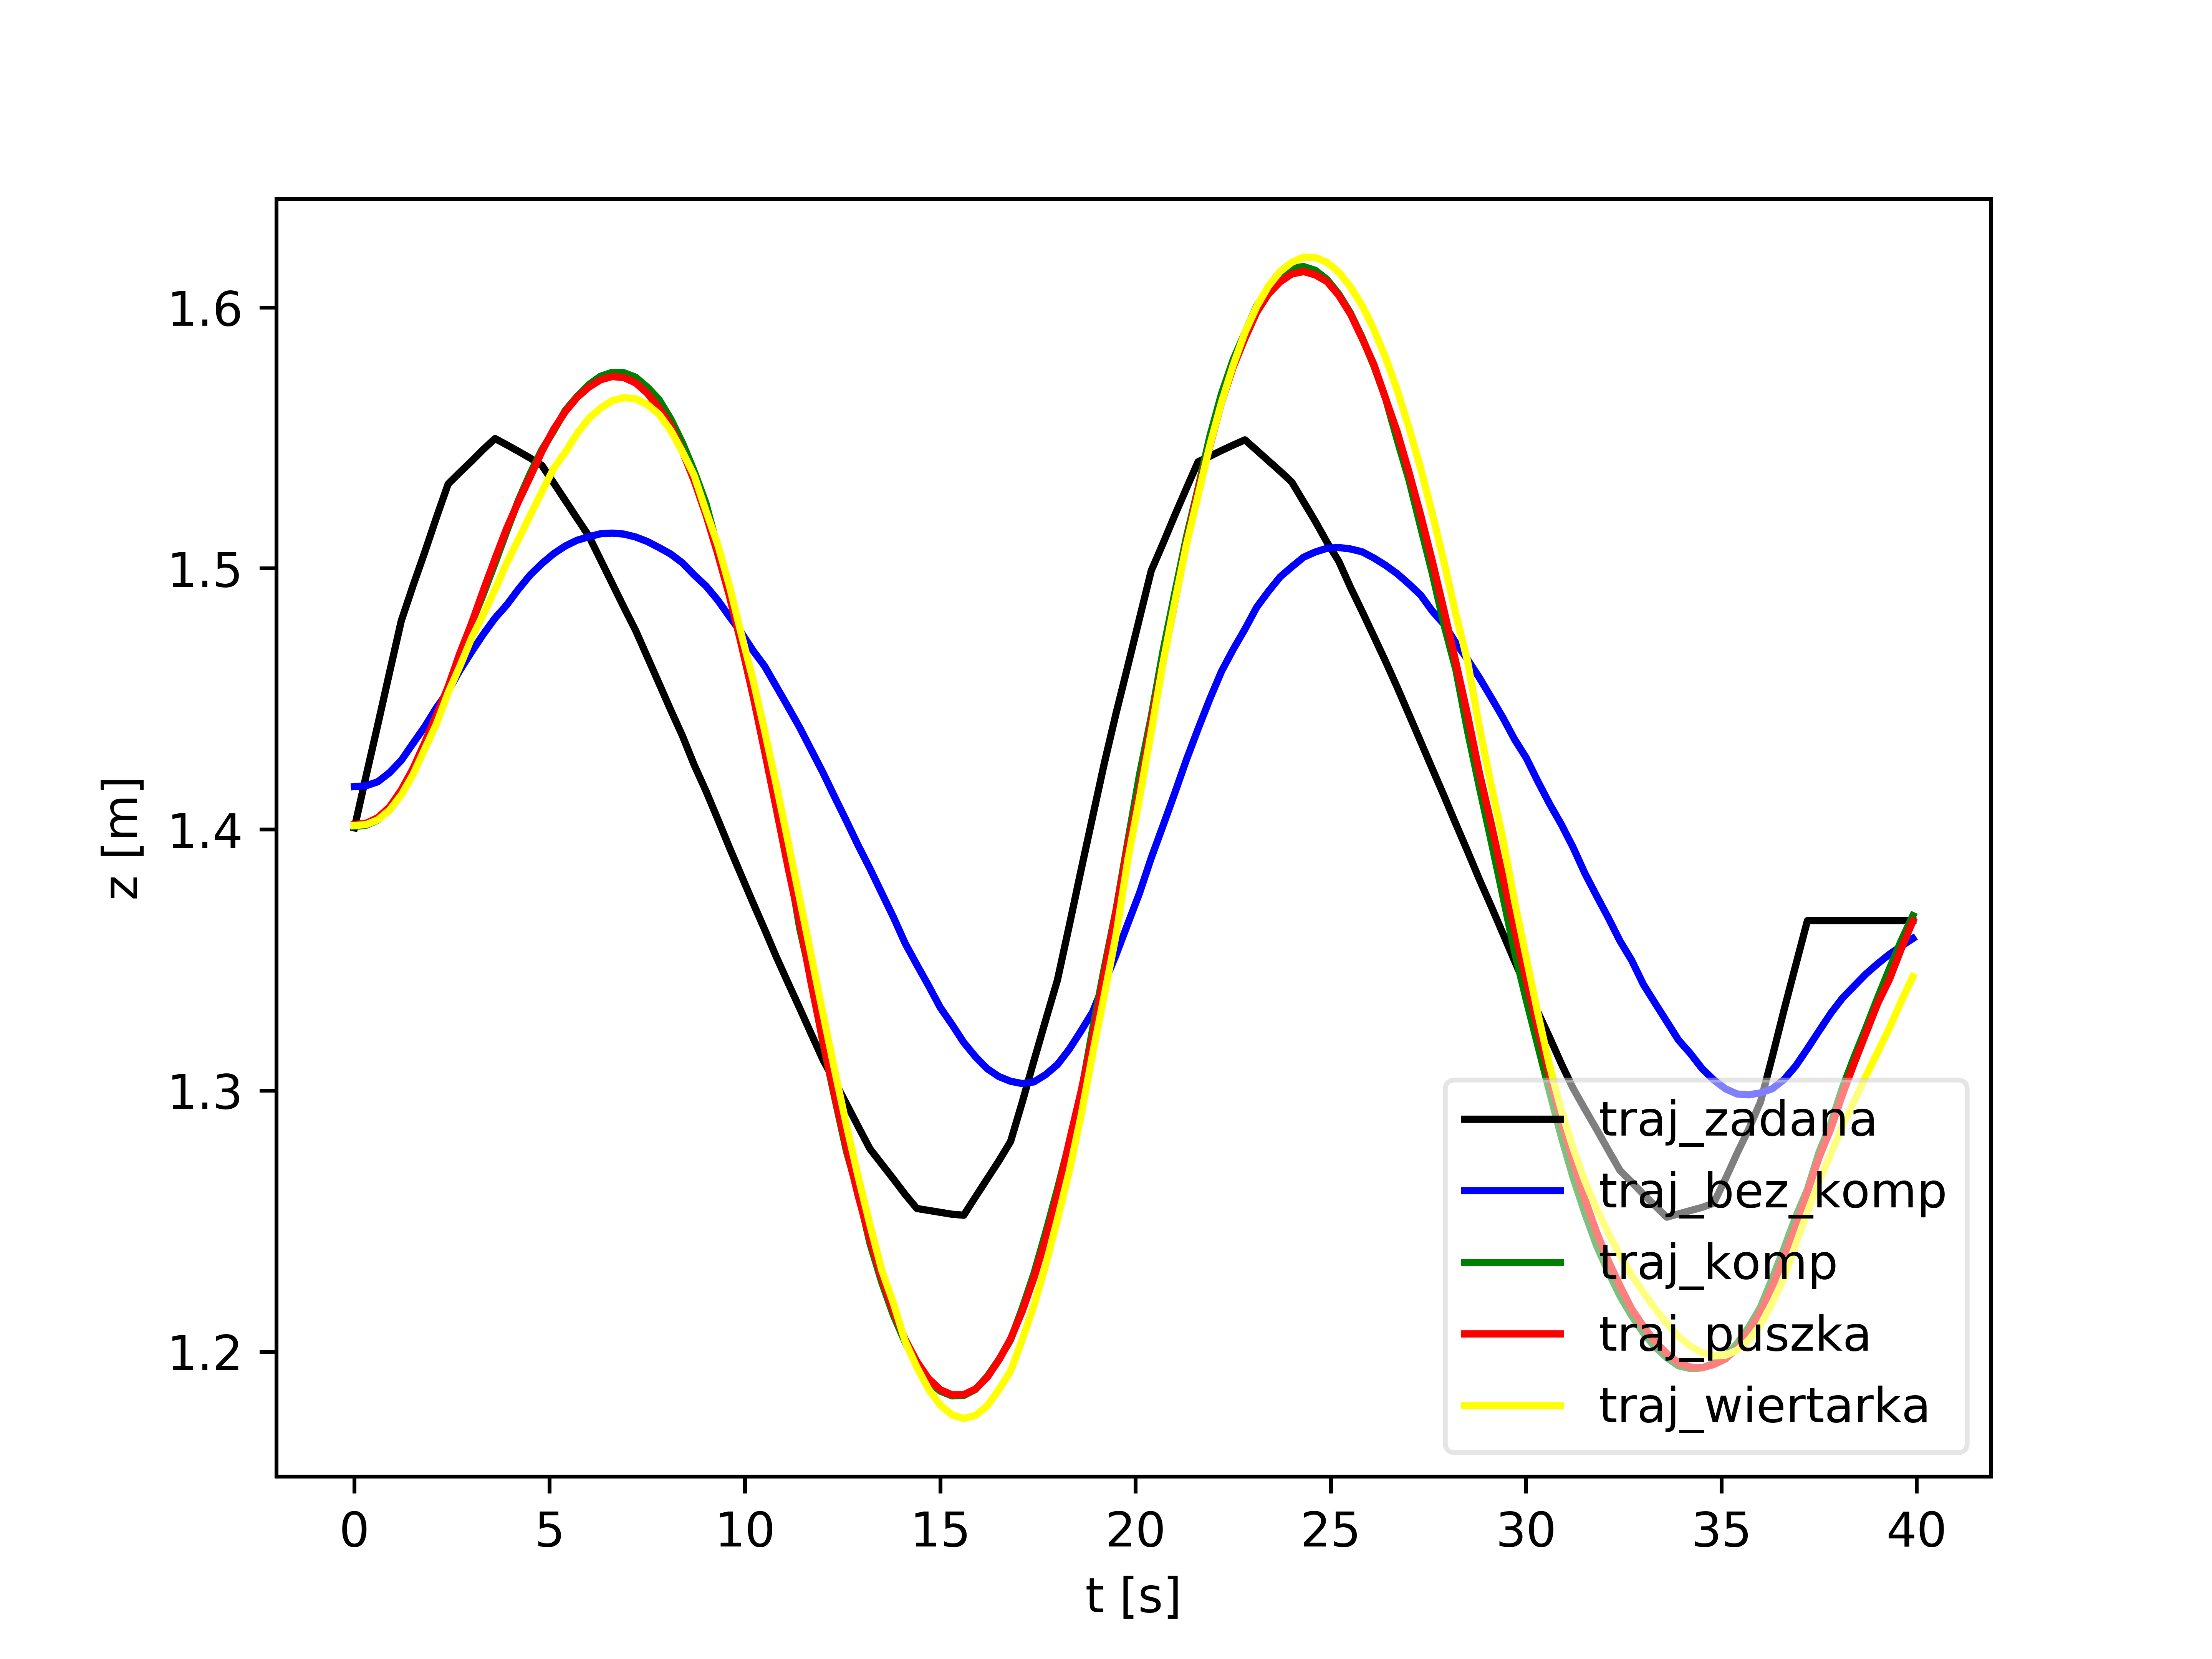
\includegraphics[width=.45\textwidth]{../../velma/przerobione_testy/out/osemka/common_az.png}
	}

	\caption{Ruch osemkowy. Porownanie trajektorii pozycji w zaleznosci od czasu.}
	\label{fig:osemka_a}

\end{figure}


\begin{figure}[h]
	\centering
	\subfigure[Kat osi $X$]{
		\label{fig:osemka_rotx}
		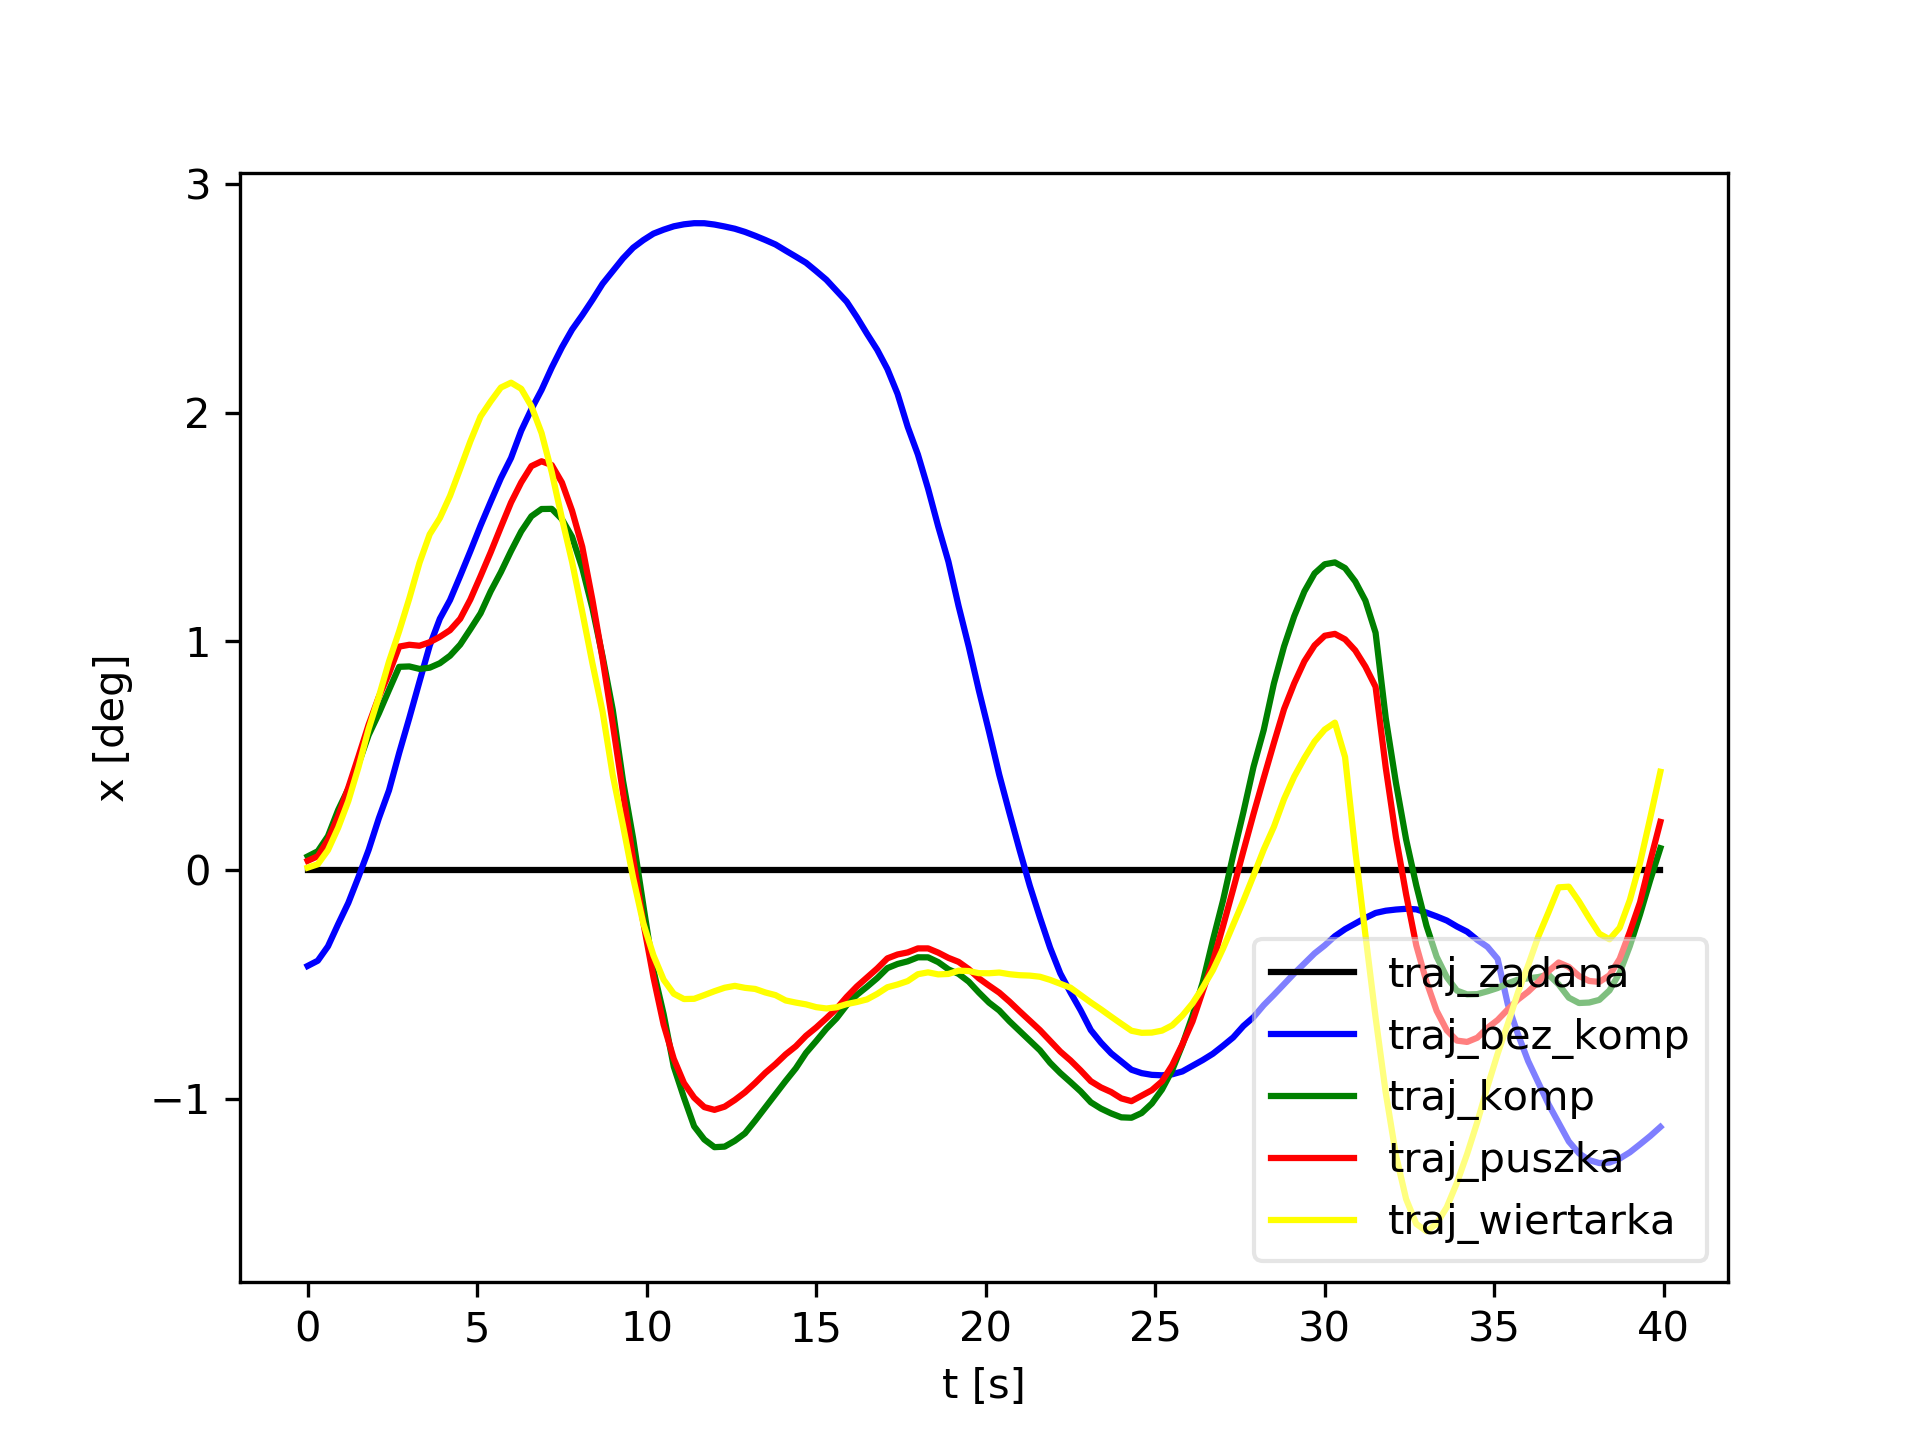
\includegraphics[width=.45\textwidth]{../../velma/przerobione_testy/out/osemka/common_rotx.png}
	}
	\hfill
	\subfigure[Kat osi $Y$]{
		\label{fig:do_gory_roty}
		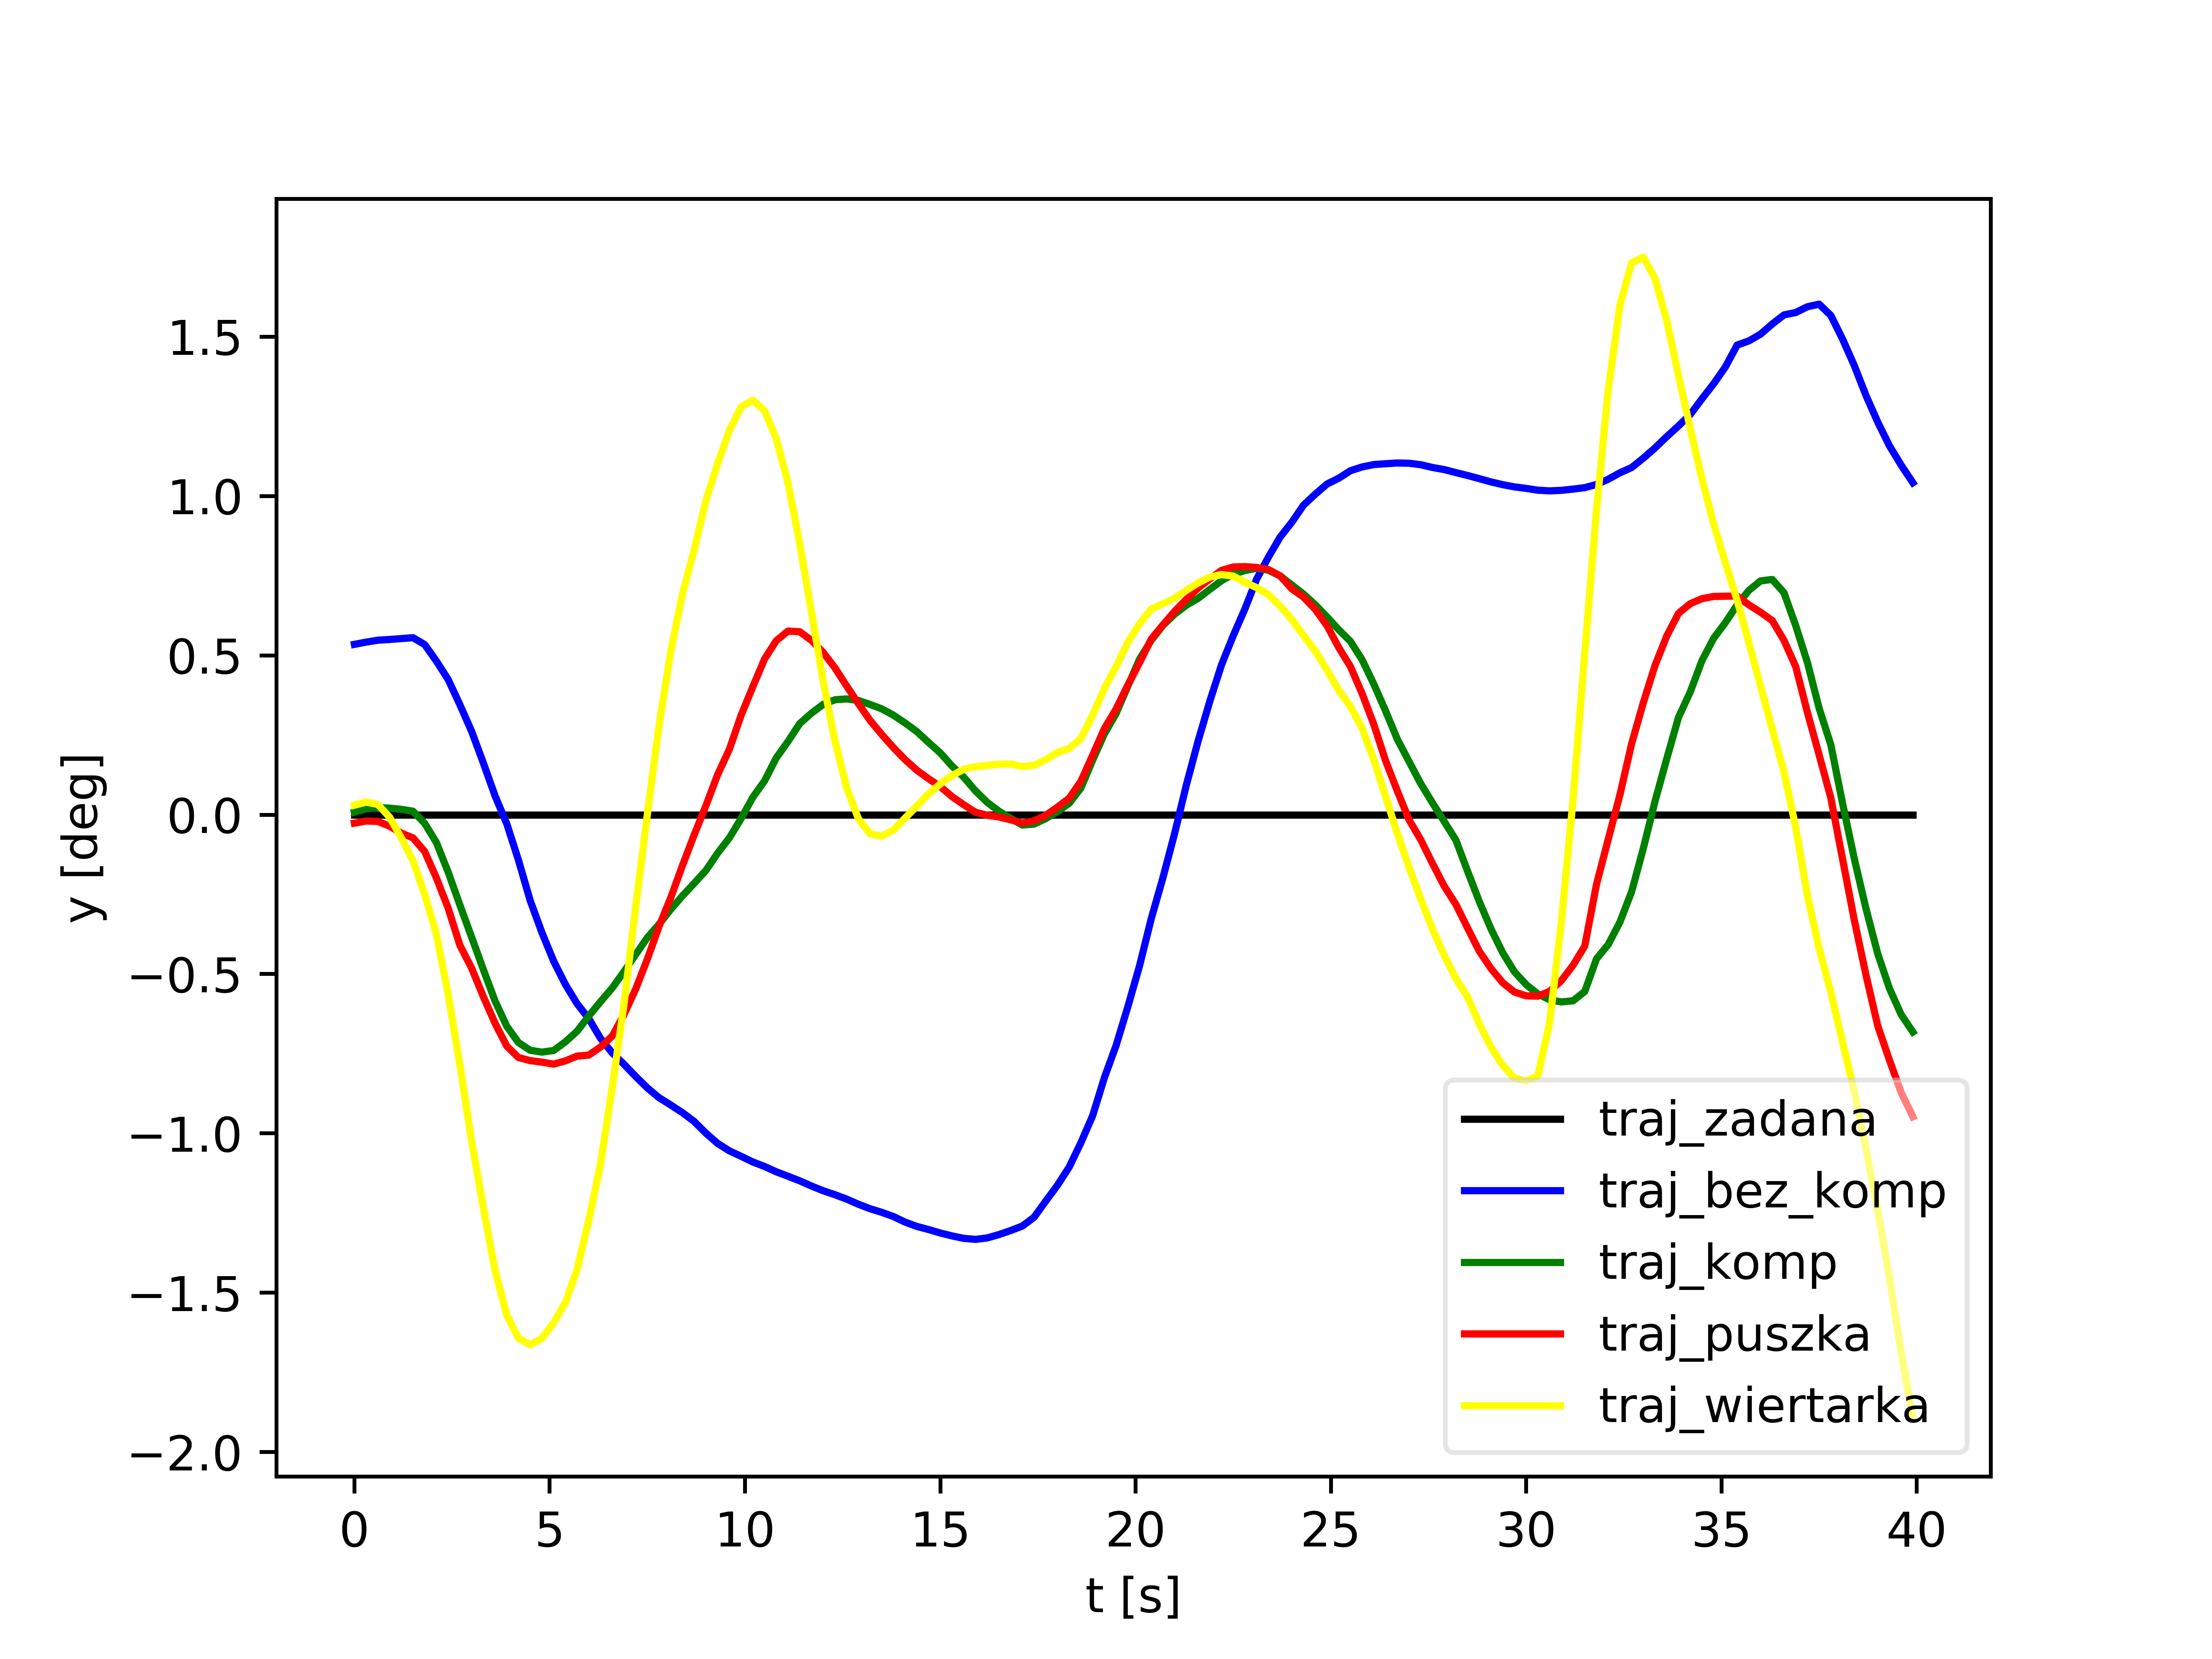
\includegraphics[width=.45\textwidth]{../../velma/przerobione_testy/out/osemka/common_roty.png}
	}
	
	\hfill
	\subfigure[Kat osi $Z$]{
		\label{fig:osemka_rotz}
		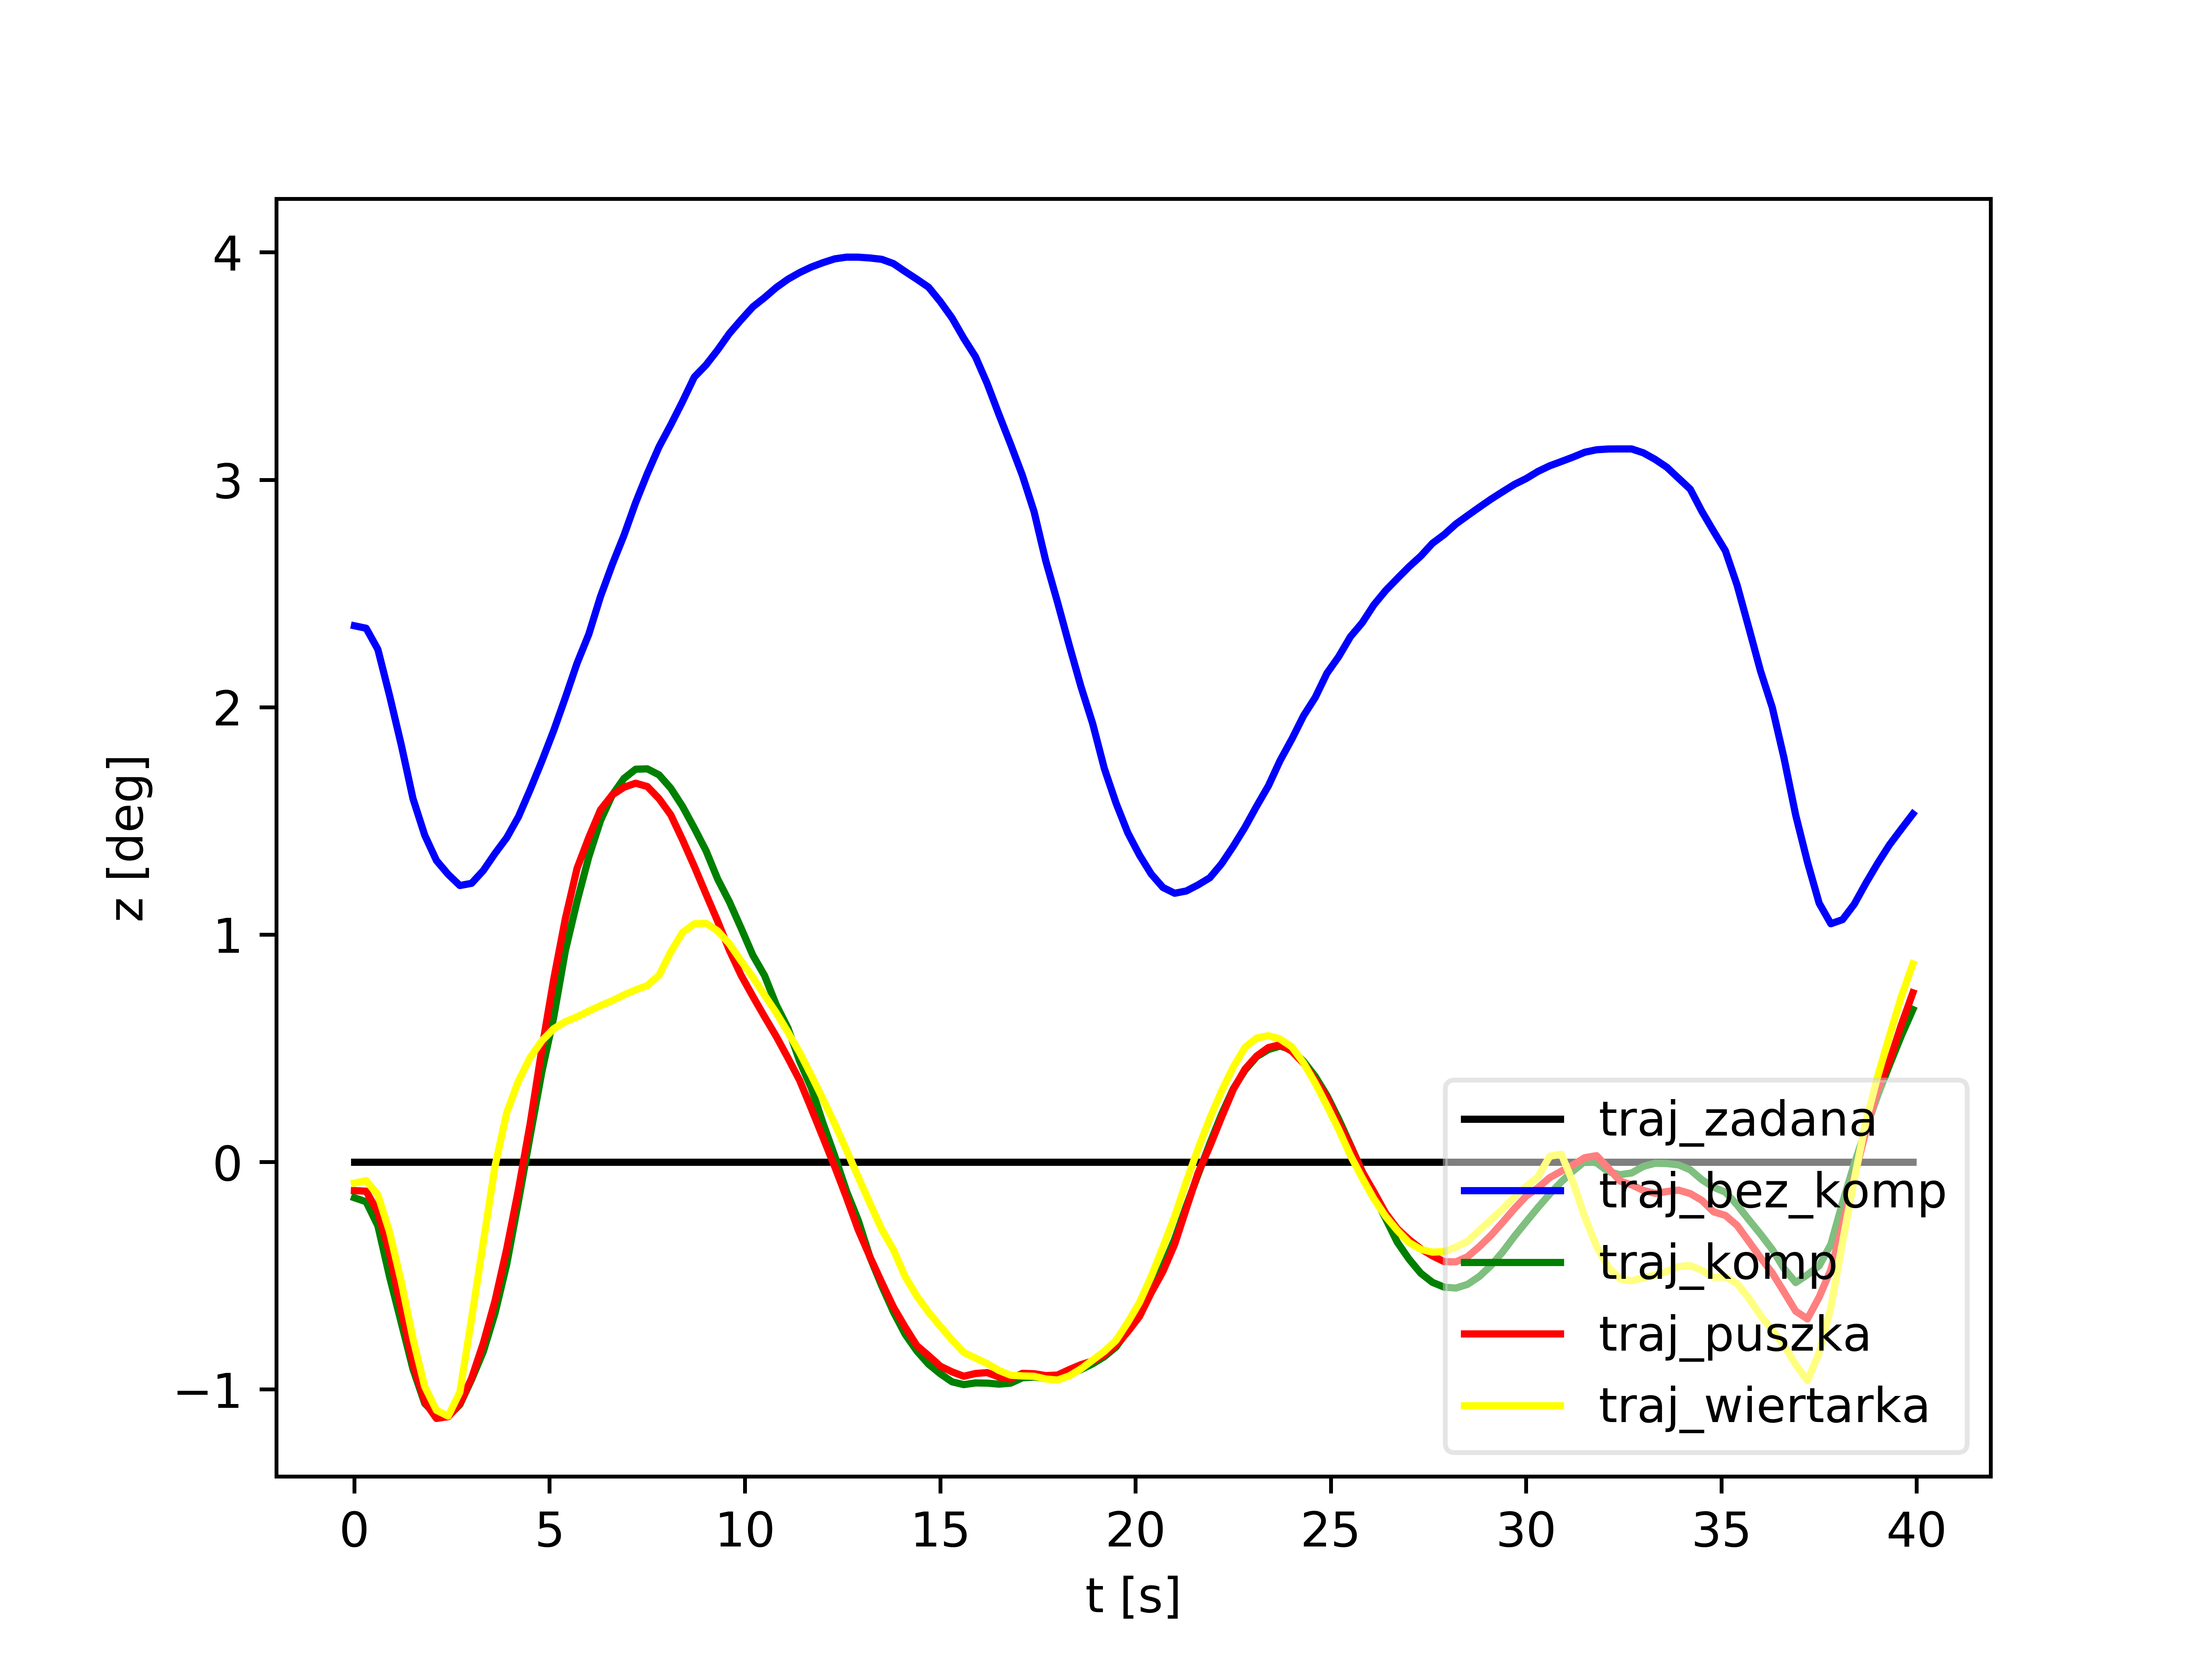
\includegraphics[width=.45\textwidth]{../../velma/przerobione_testy/out/osemka/common_rotz.png}
	}

	\caption{Ruch osemkowy. Porownanie trajektorii katow w notacji Eulera w zaleznosci od czasu.}
	\label{fig:osemka_rot}

\end{figure}

\begin{figure}
	\centering
	\subfigure[Brak algorytmu kompensacji]{
		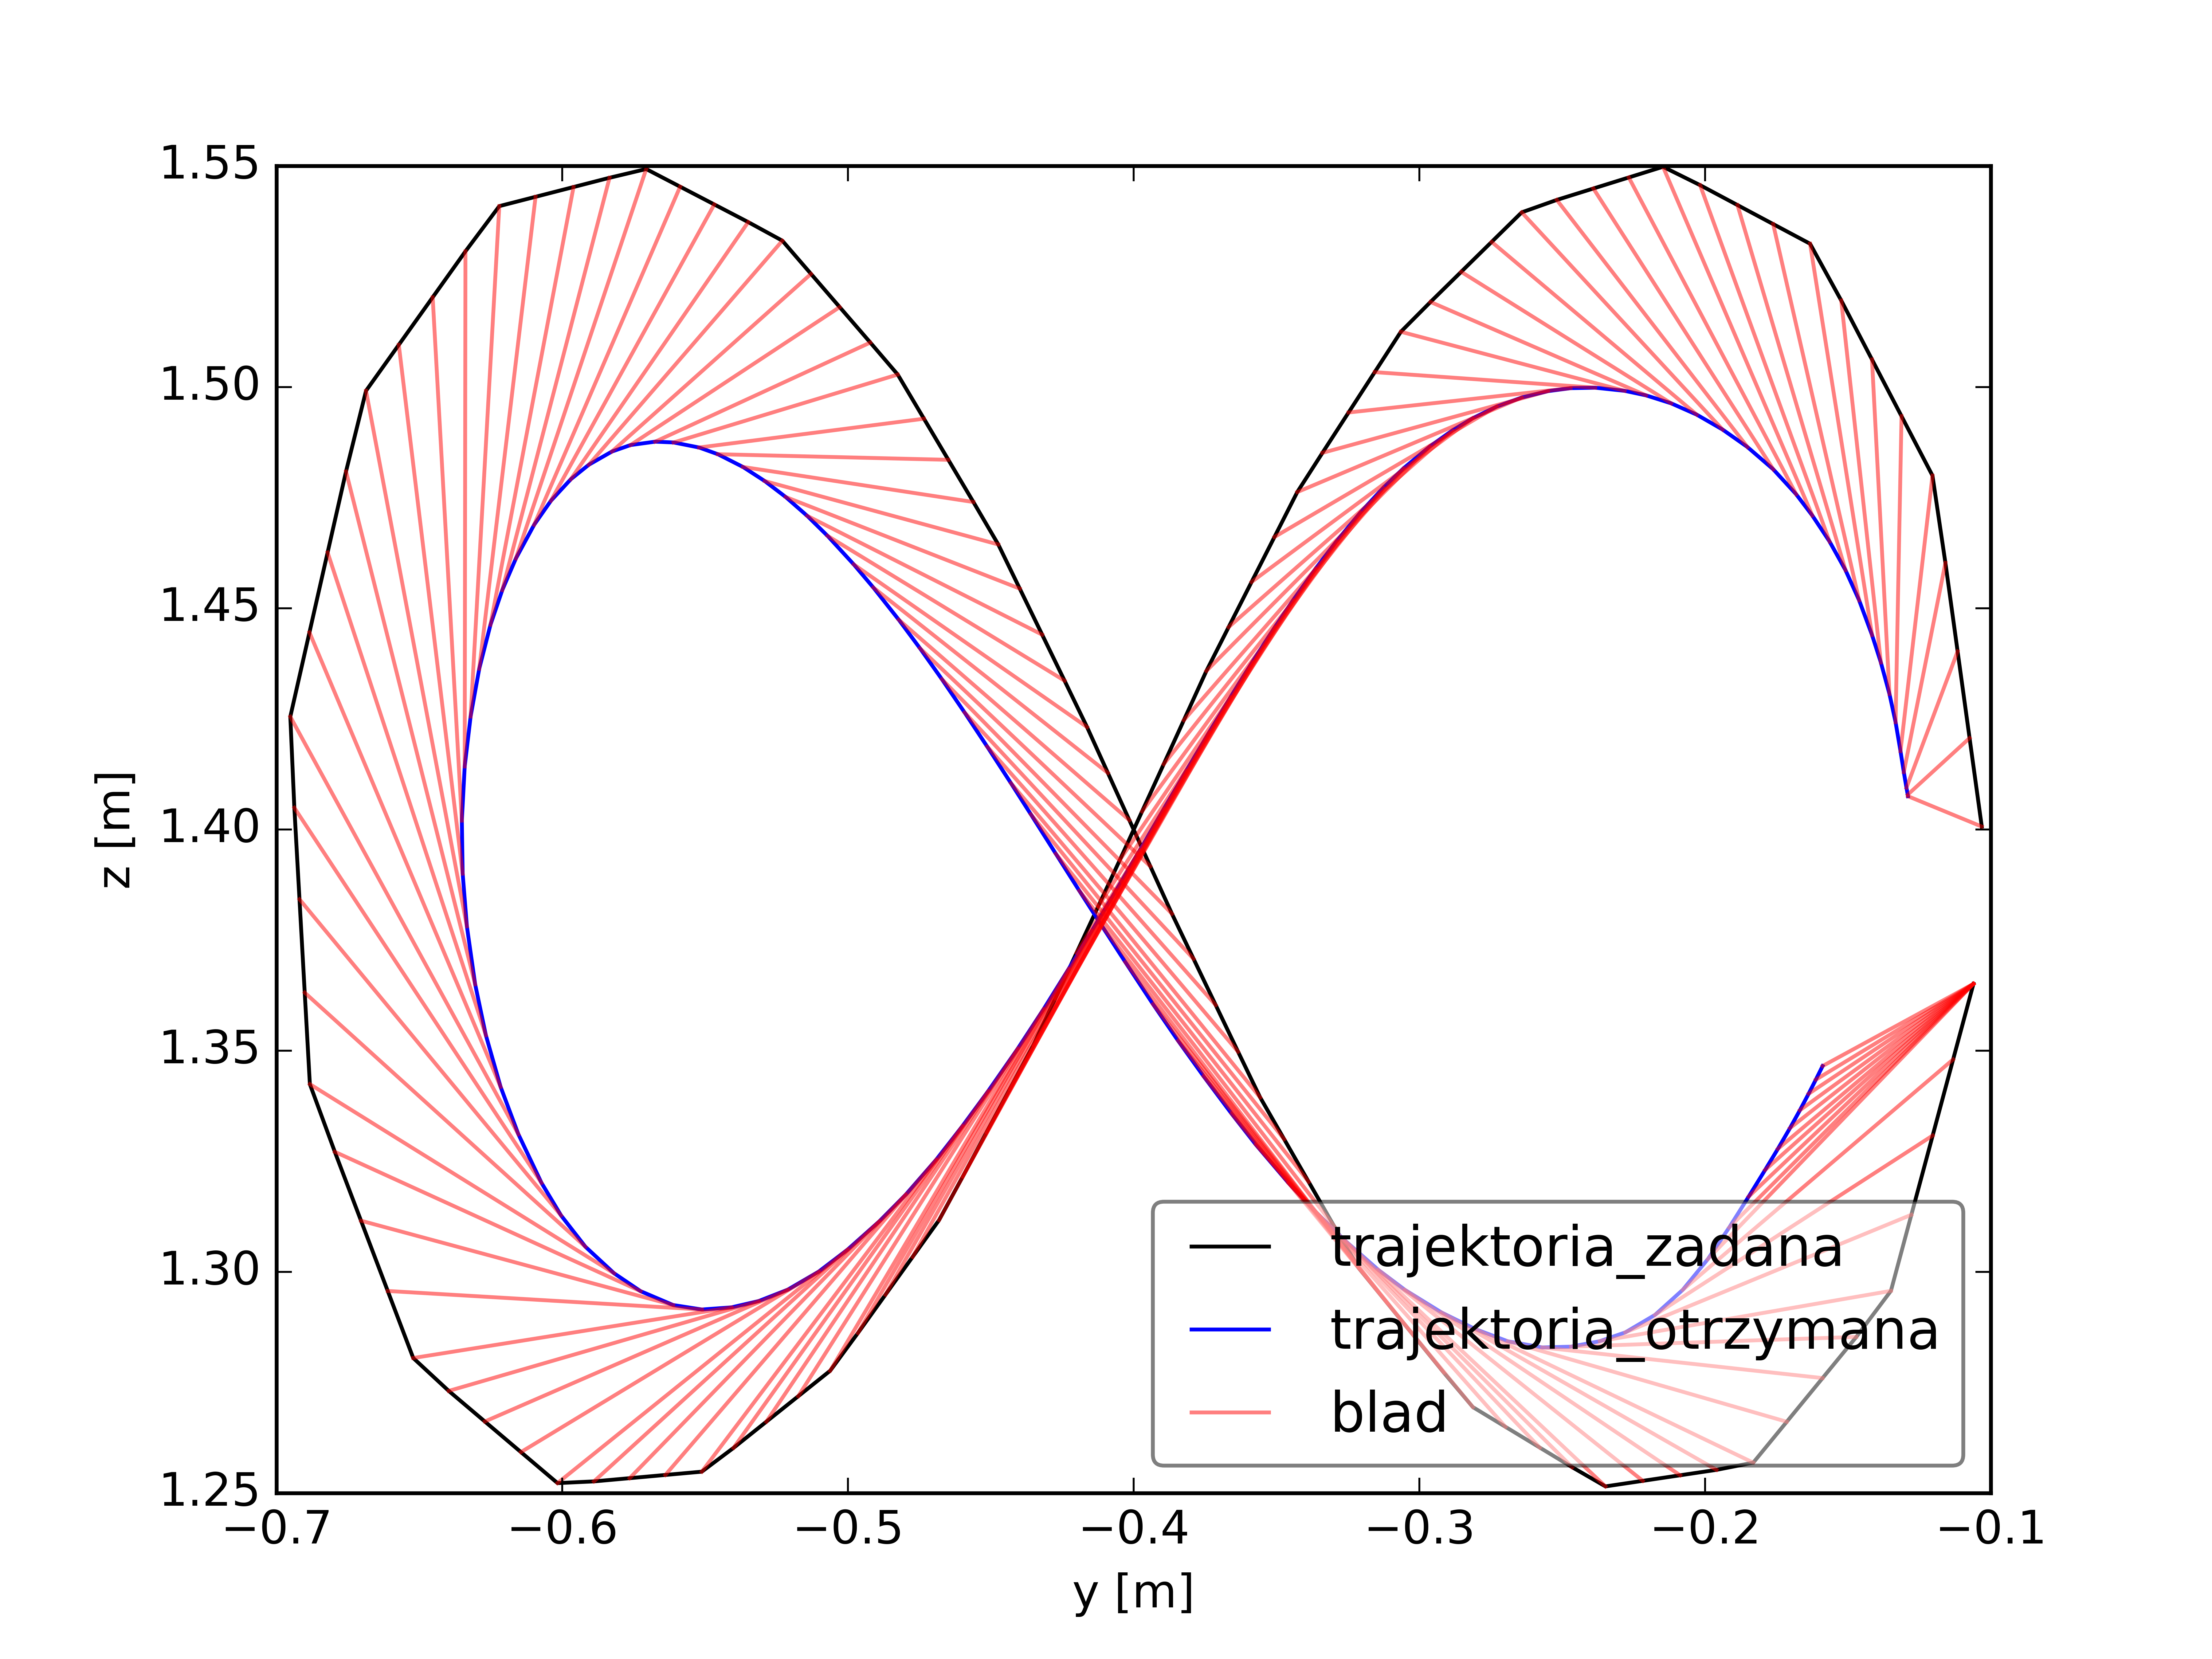
\includegraphics[width=.45\textwidth]{../../velma/przerobione_testy/out/osemka/yz_ate_plot_podnoszenie_miekki_bez_brak.png}
	}
	\hfill
	\subfigure[Zalaczony algorytm kompnesacji]{
		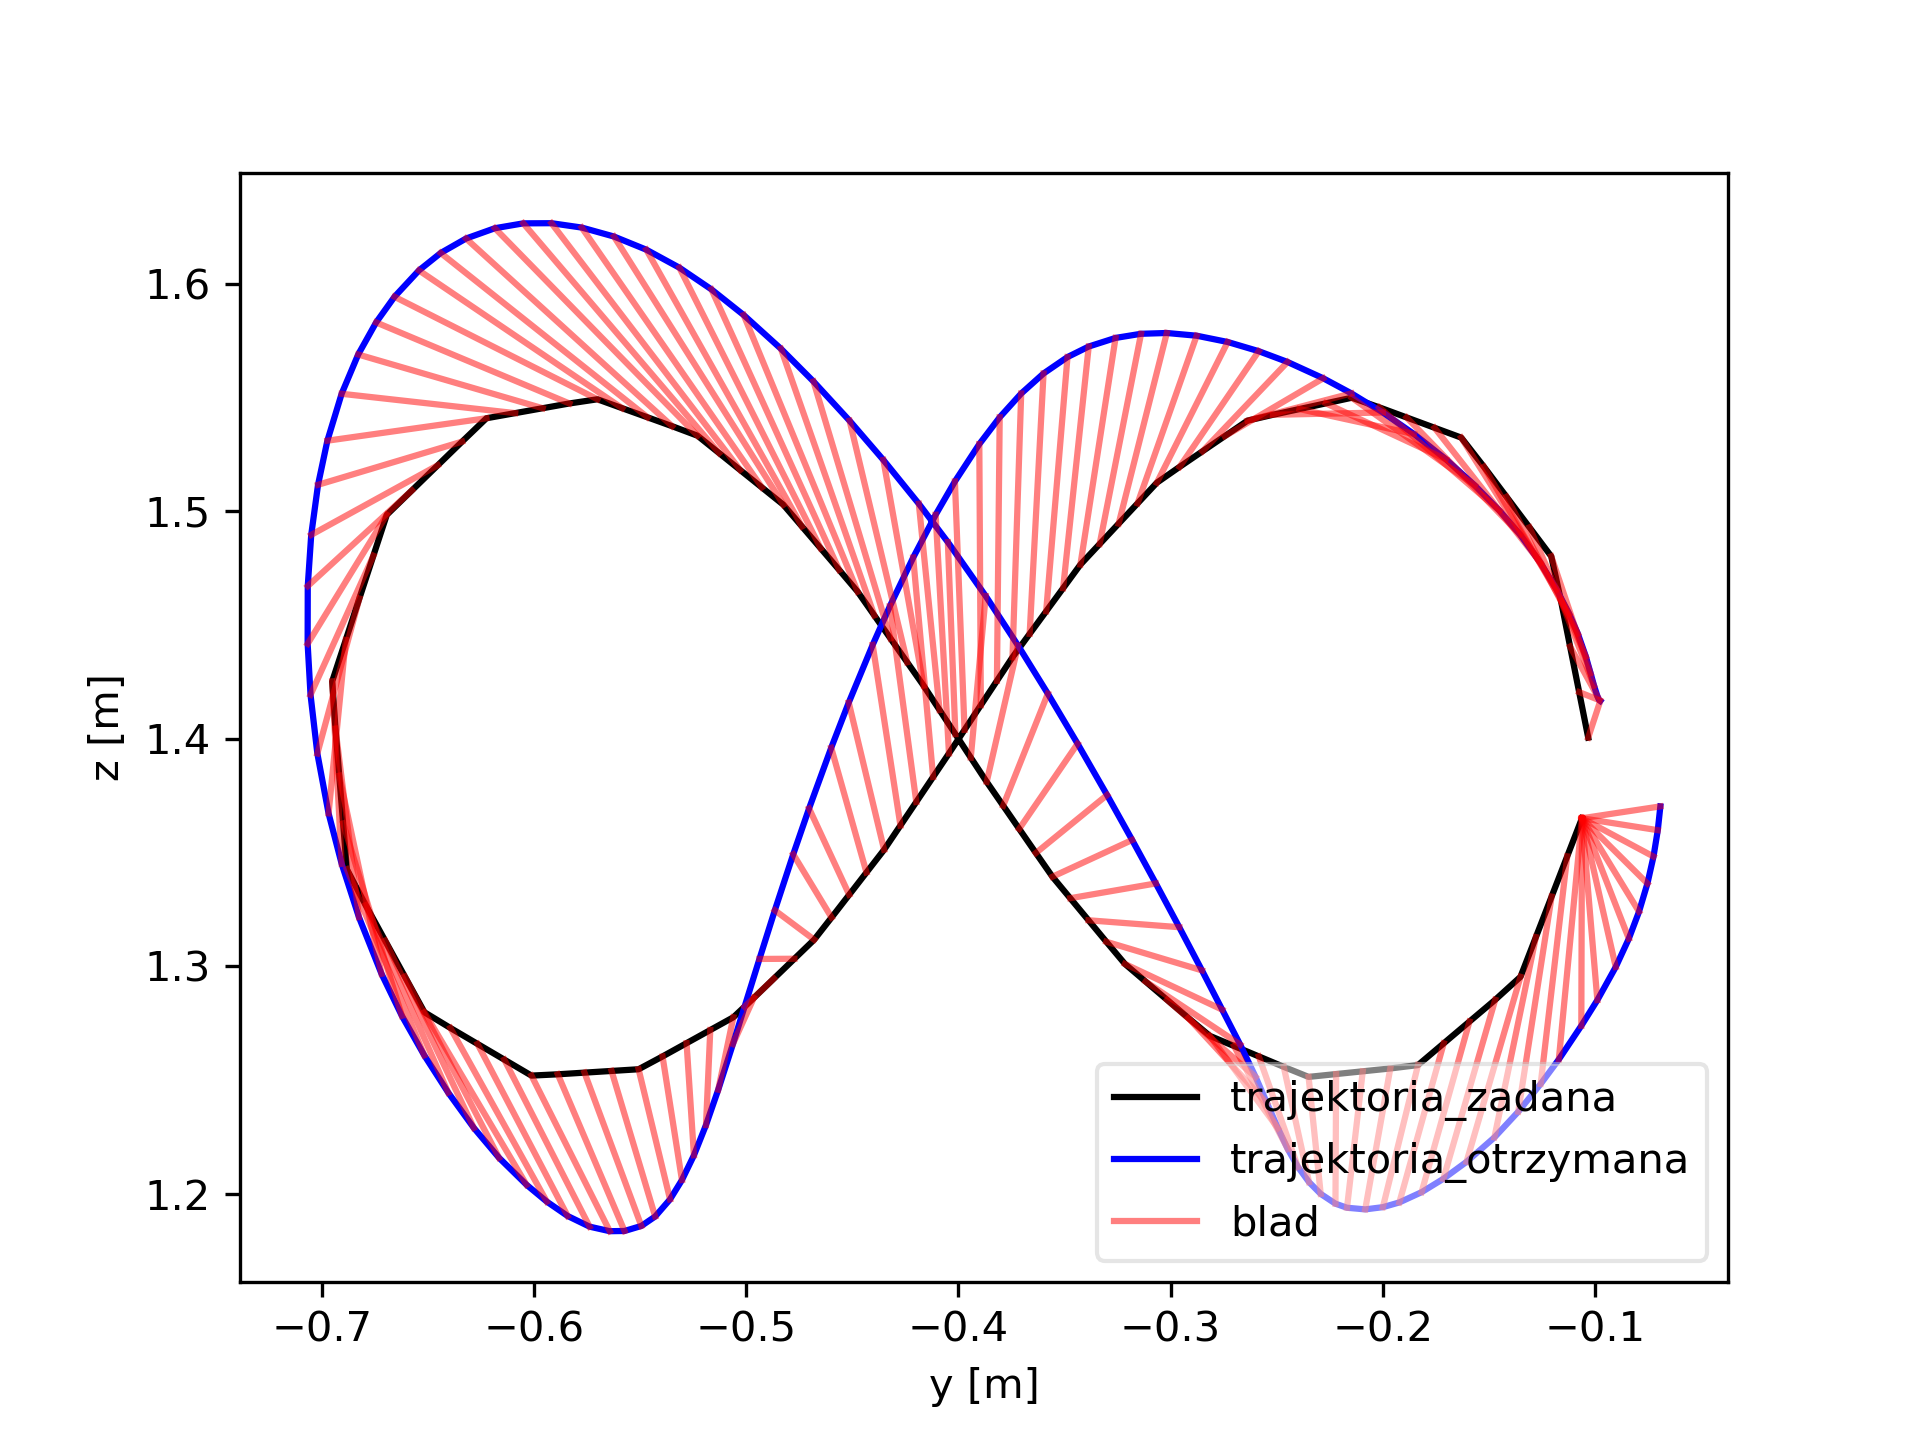
\includegraphics[width=.45\textwidth]{../../velma/przerobione_testy/out/osemka/yz_ate_plot_podnoszenie_miekki_komp_brak.png}
	}
	\caption{Porownanie trajektorii chwytaka w osiach $Y$ i $Z$}
	\label{fig:osemka_porow_komp}
\end{figure}

\begin{figure}
	\centering
	\subfigure[Trajektoria z chwycona puszka]{
		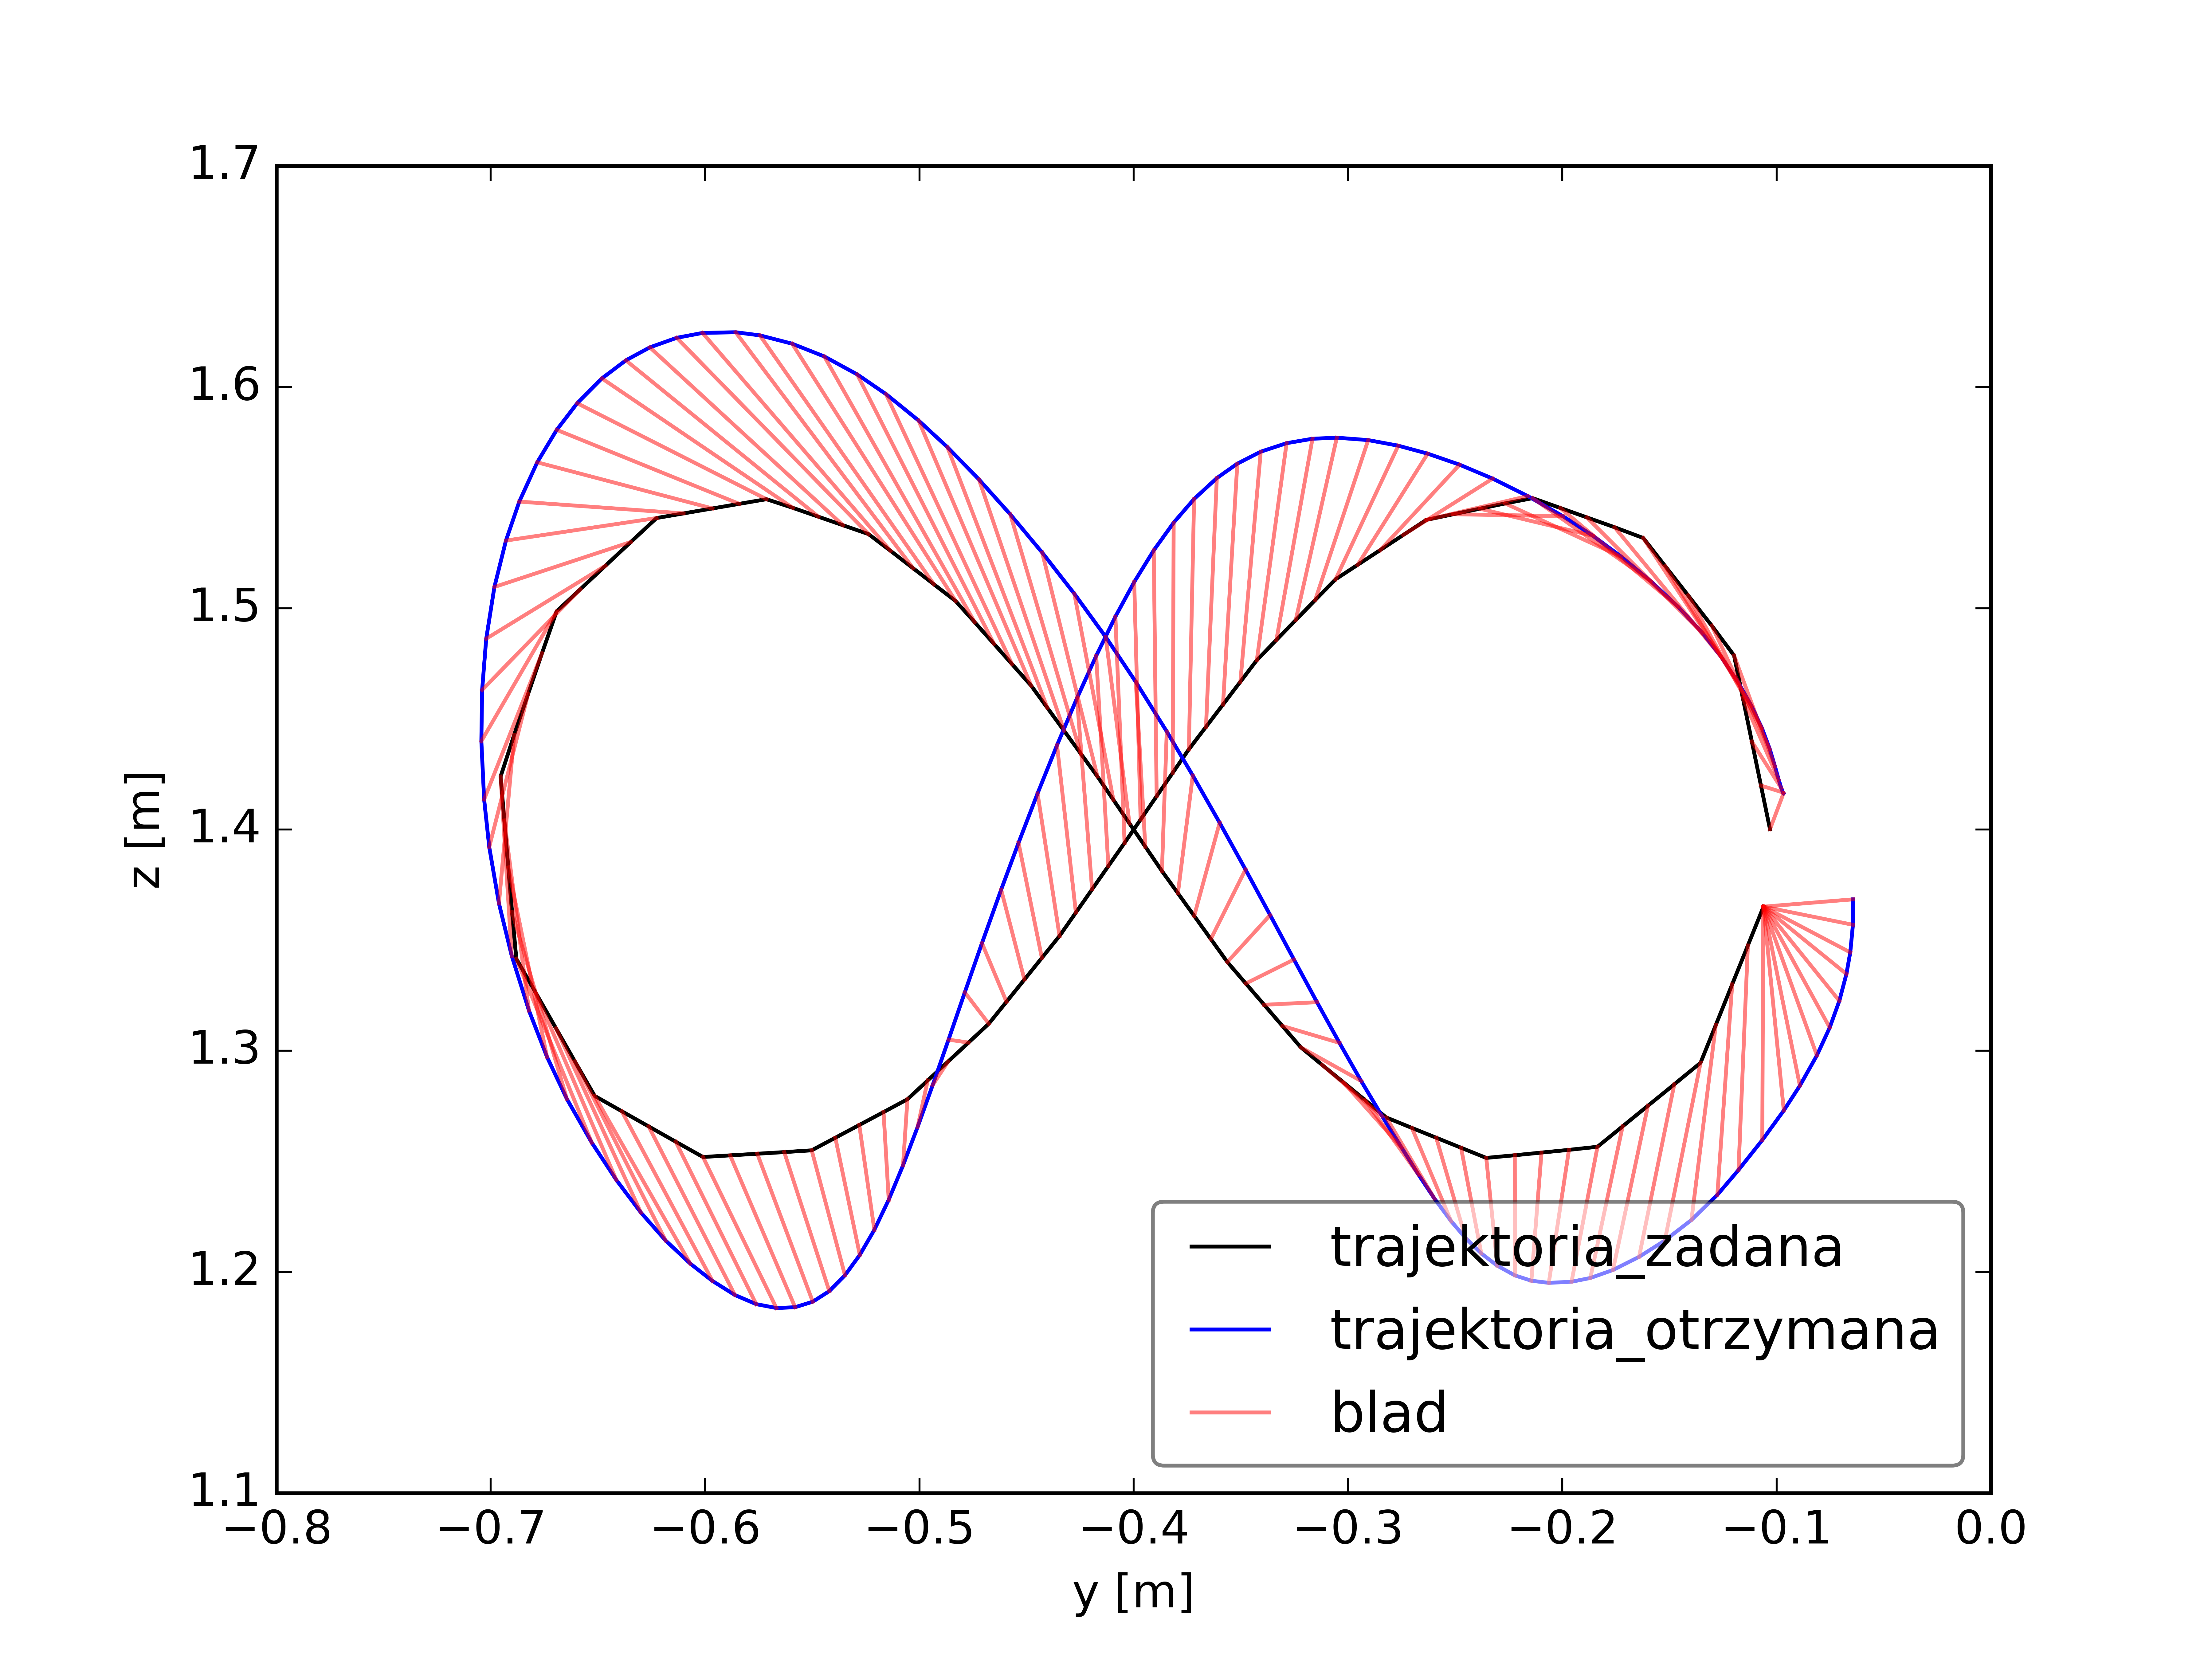
\includegraphics[width=.45\textwidth]{../../velma/przerobione_testy/out/osemka/yz_ate_plot_podnoszenie_miekki_komp_piwo.png}
	}
	\hfill
	\subfigure[Trajektoria z chwycona wiertarka]{
		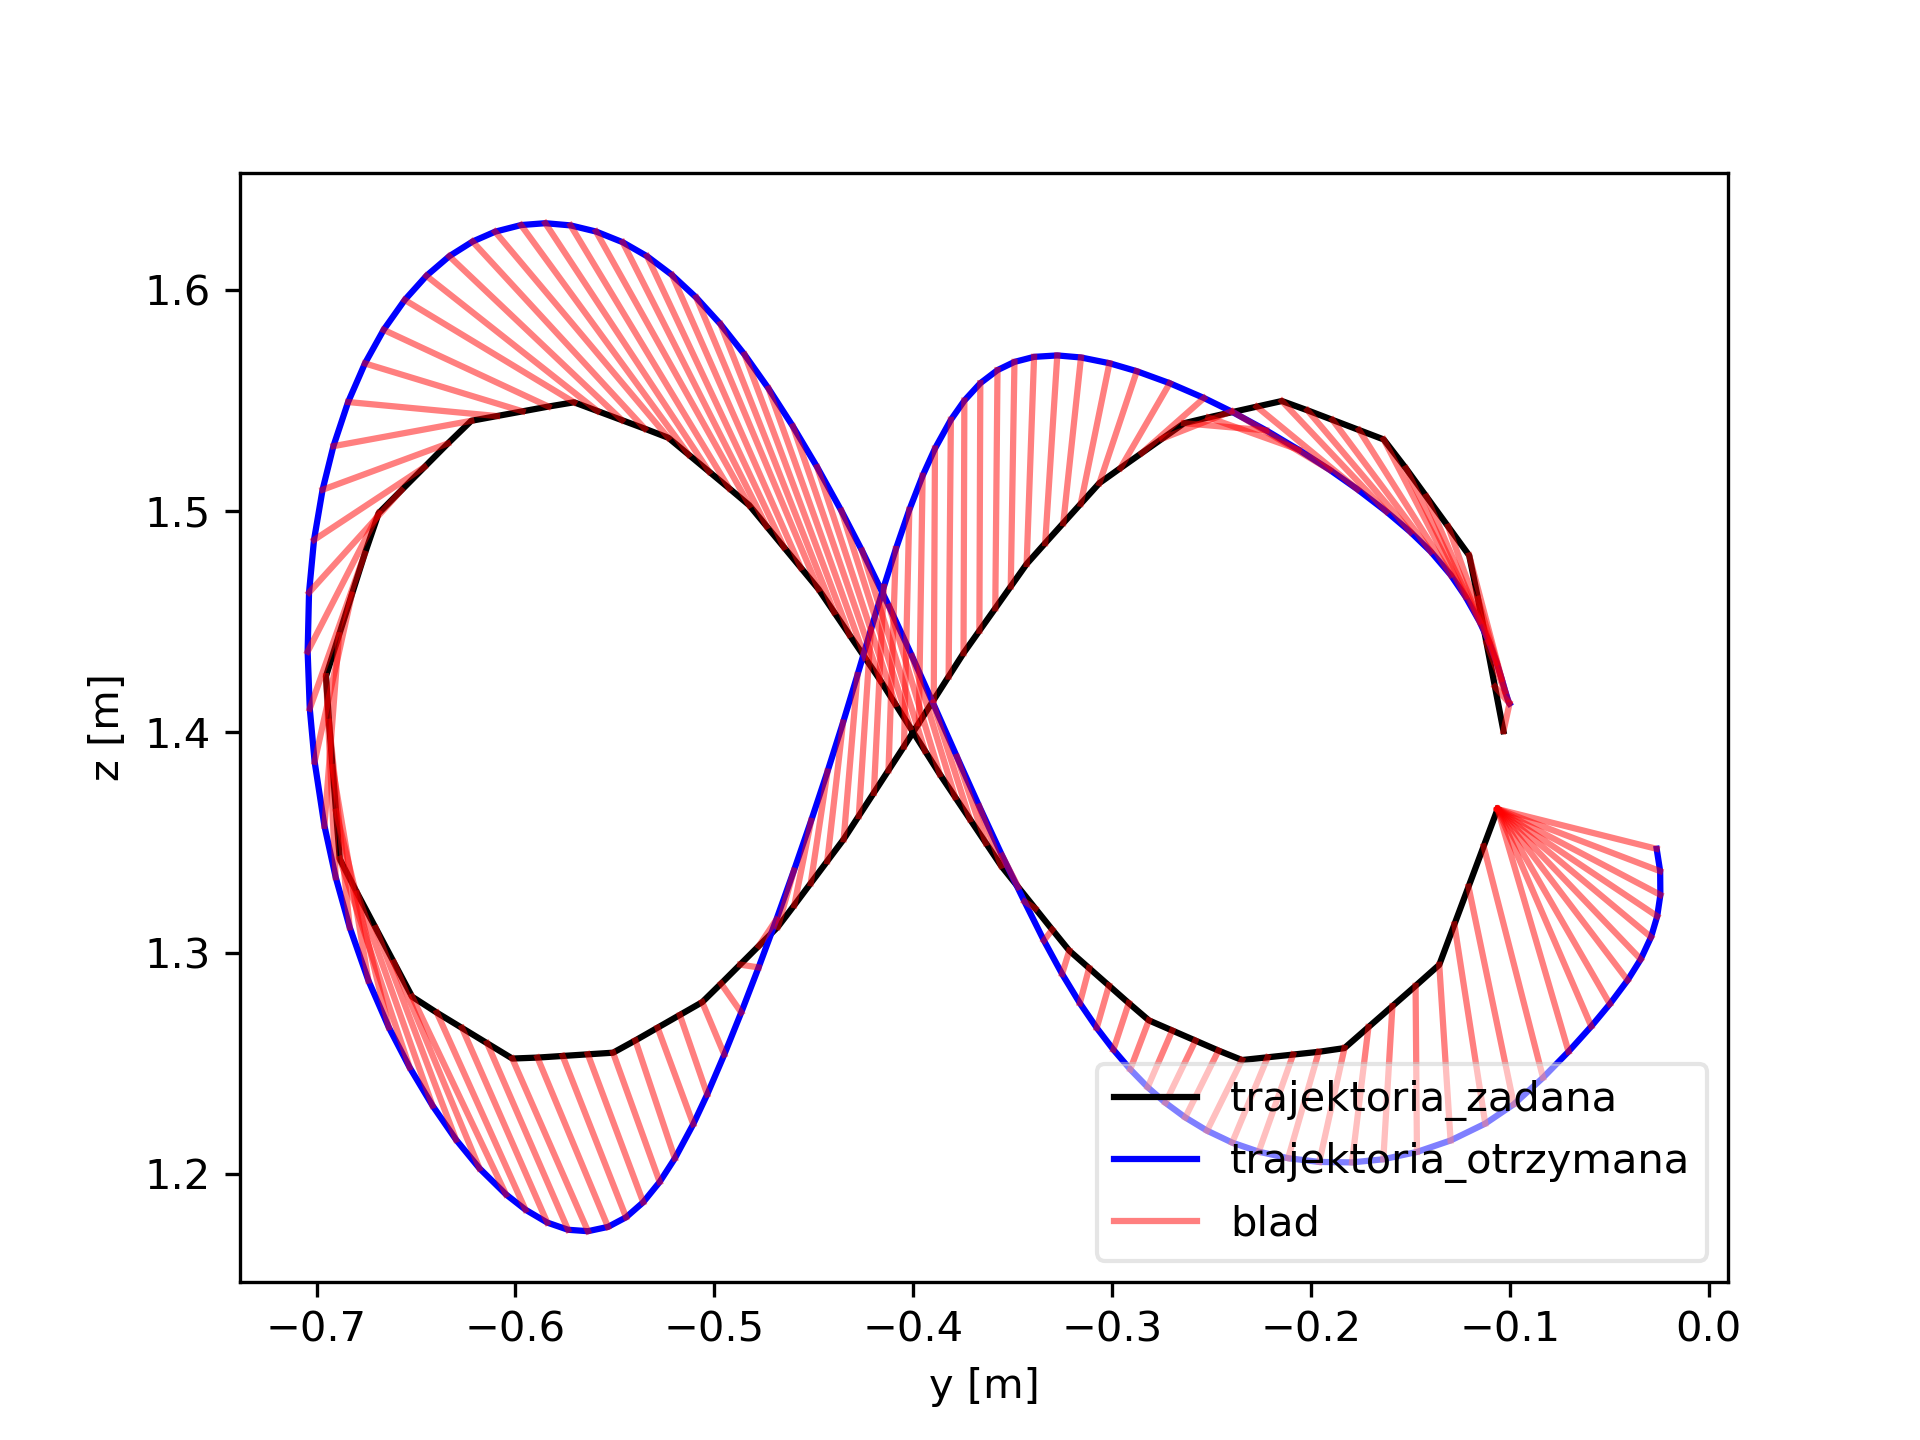
\includegraphics[width=.45\textwidth]{../../velma/przerobione_testy/out/osemka/yz_ate_plot_podnoszenie_miekki_komp_wiertarka.png}
	}
	\caption{Porownanie trajektorii chwytaka w osiach $Y$ i $Z$}
	\label{fig:osemka_porow_przedm}
\end{figure}


\begin{figure}
	\centering
	\subfigure[Brak algorytmu kompensacji]{
		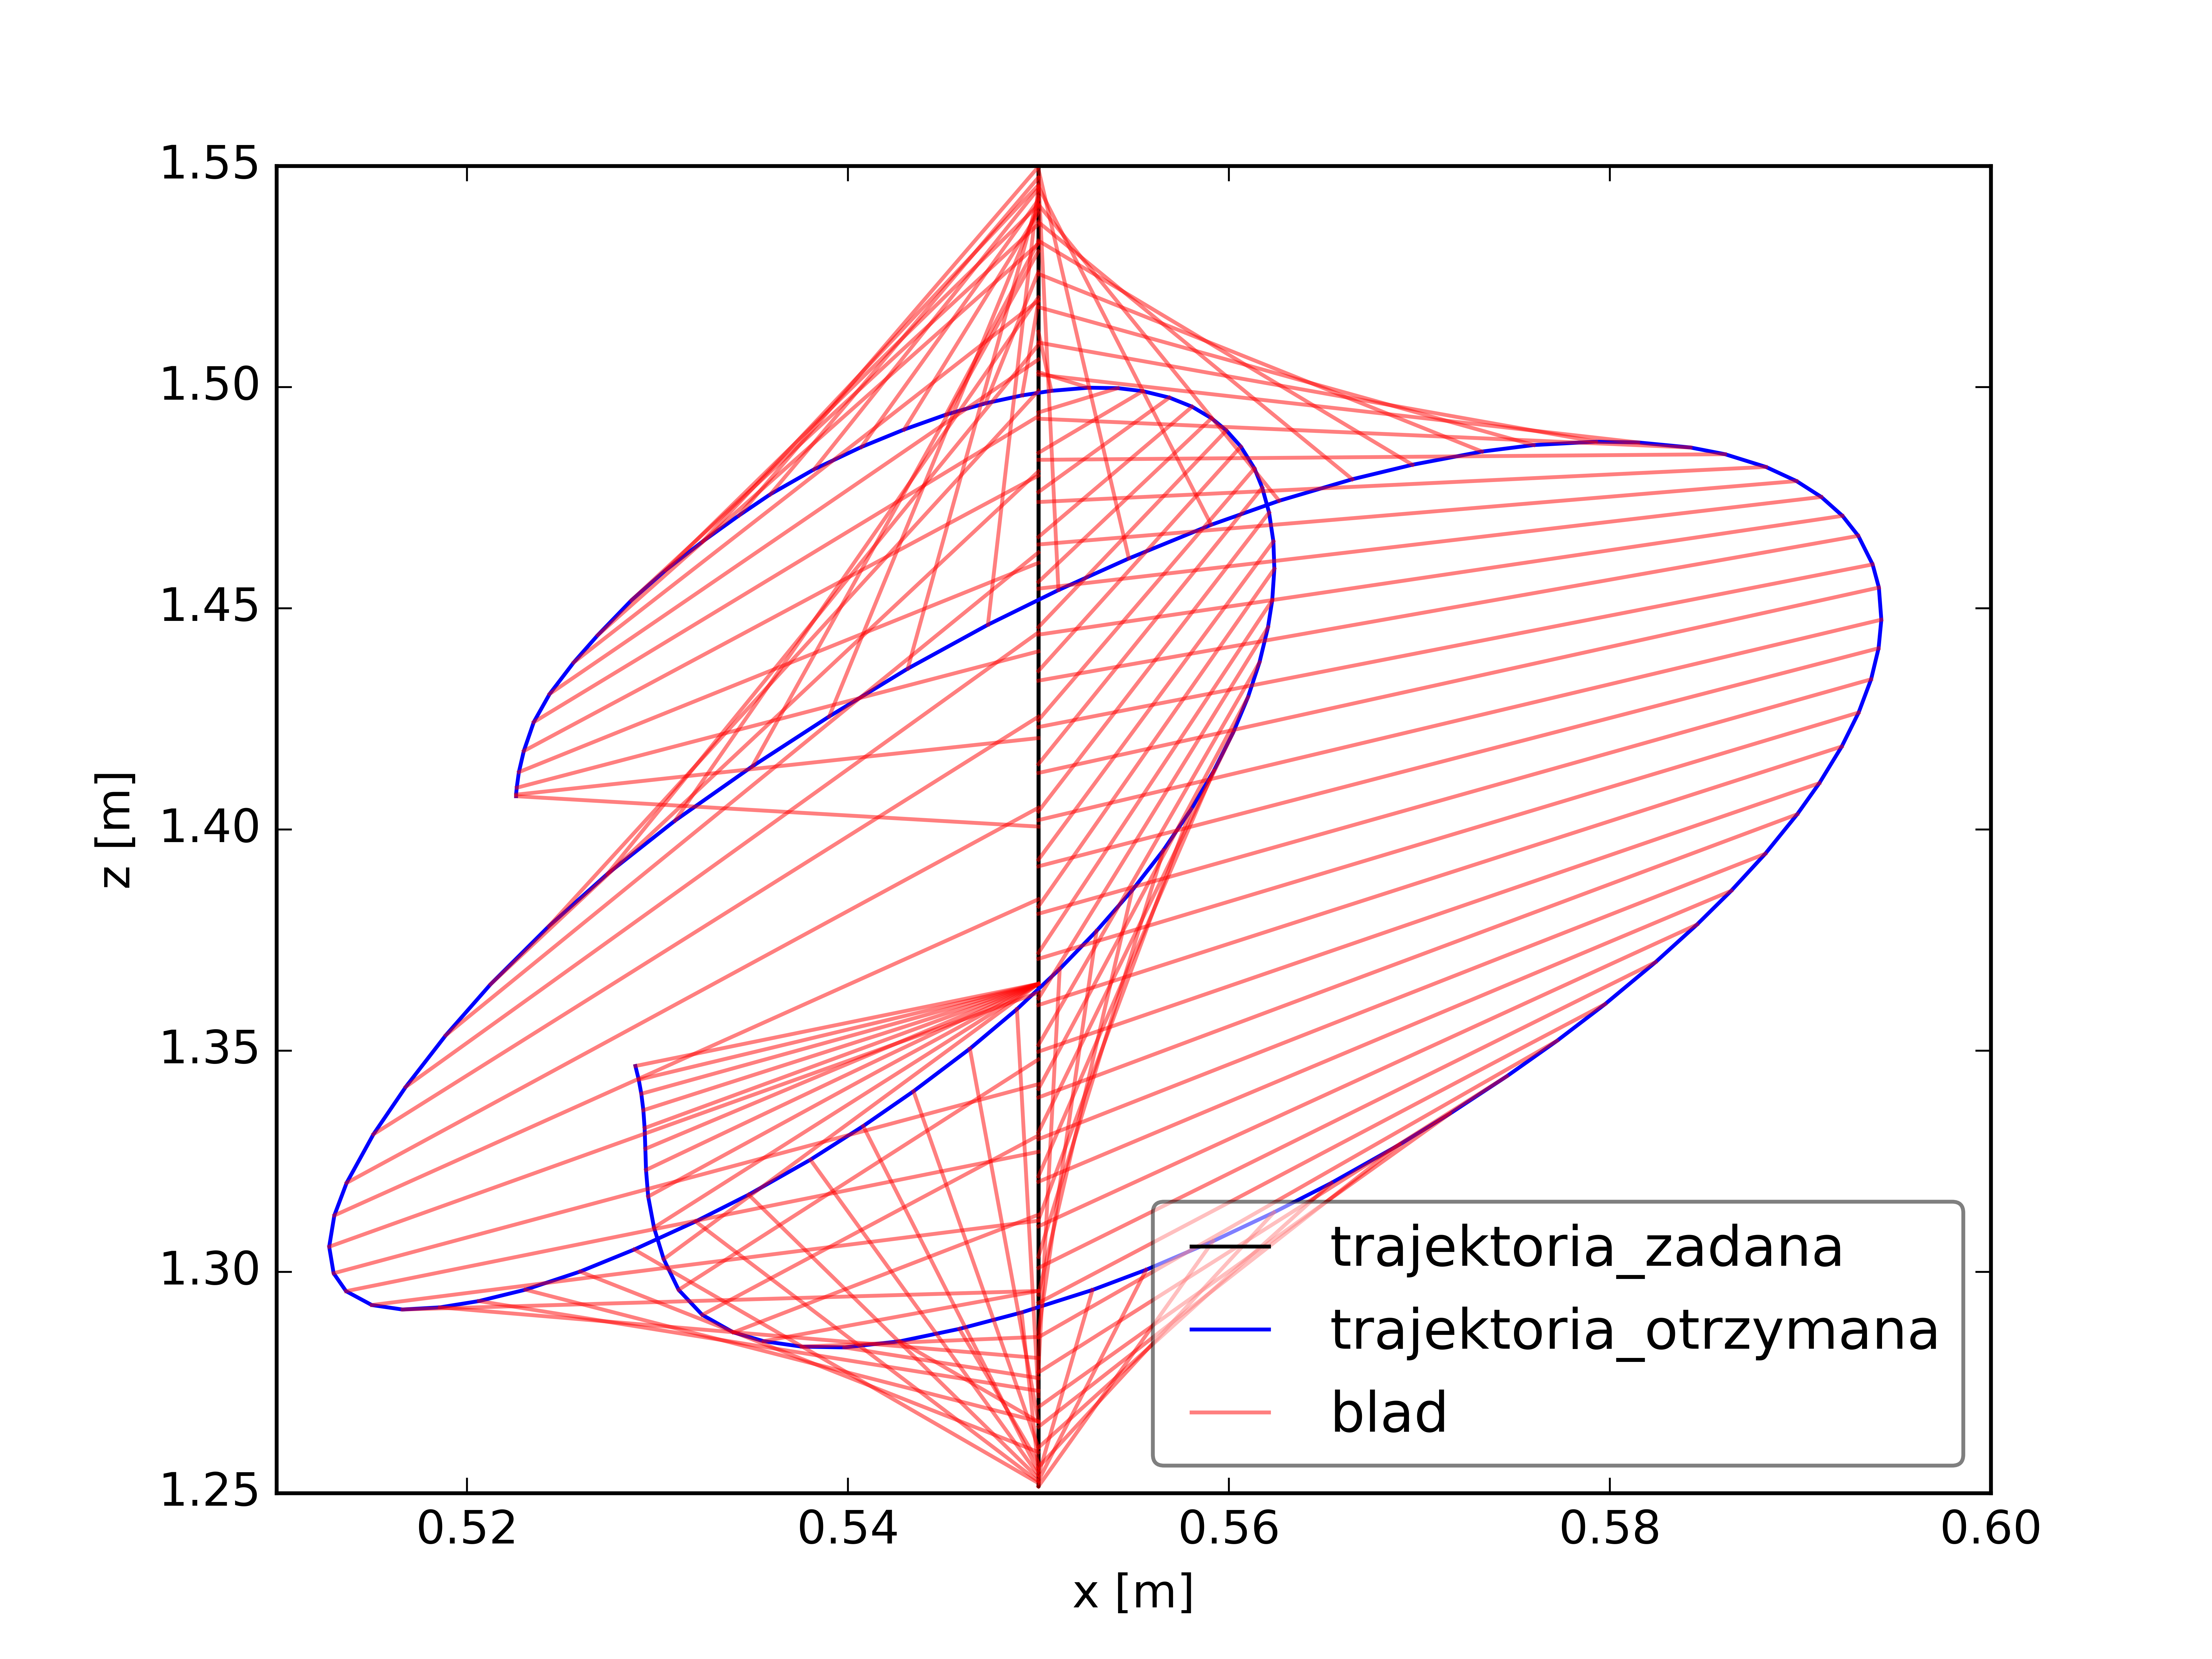
\includegraphics[width=.45\textwidth]{../../velma/przerobione_testy/out/osemka/xz_ate_plot_podnoszenie_miekki_bez_brak.png}
	}
	\hfill
	\subfigure[Zalaczony algorytm kompnesacji]{
		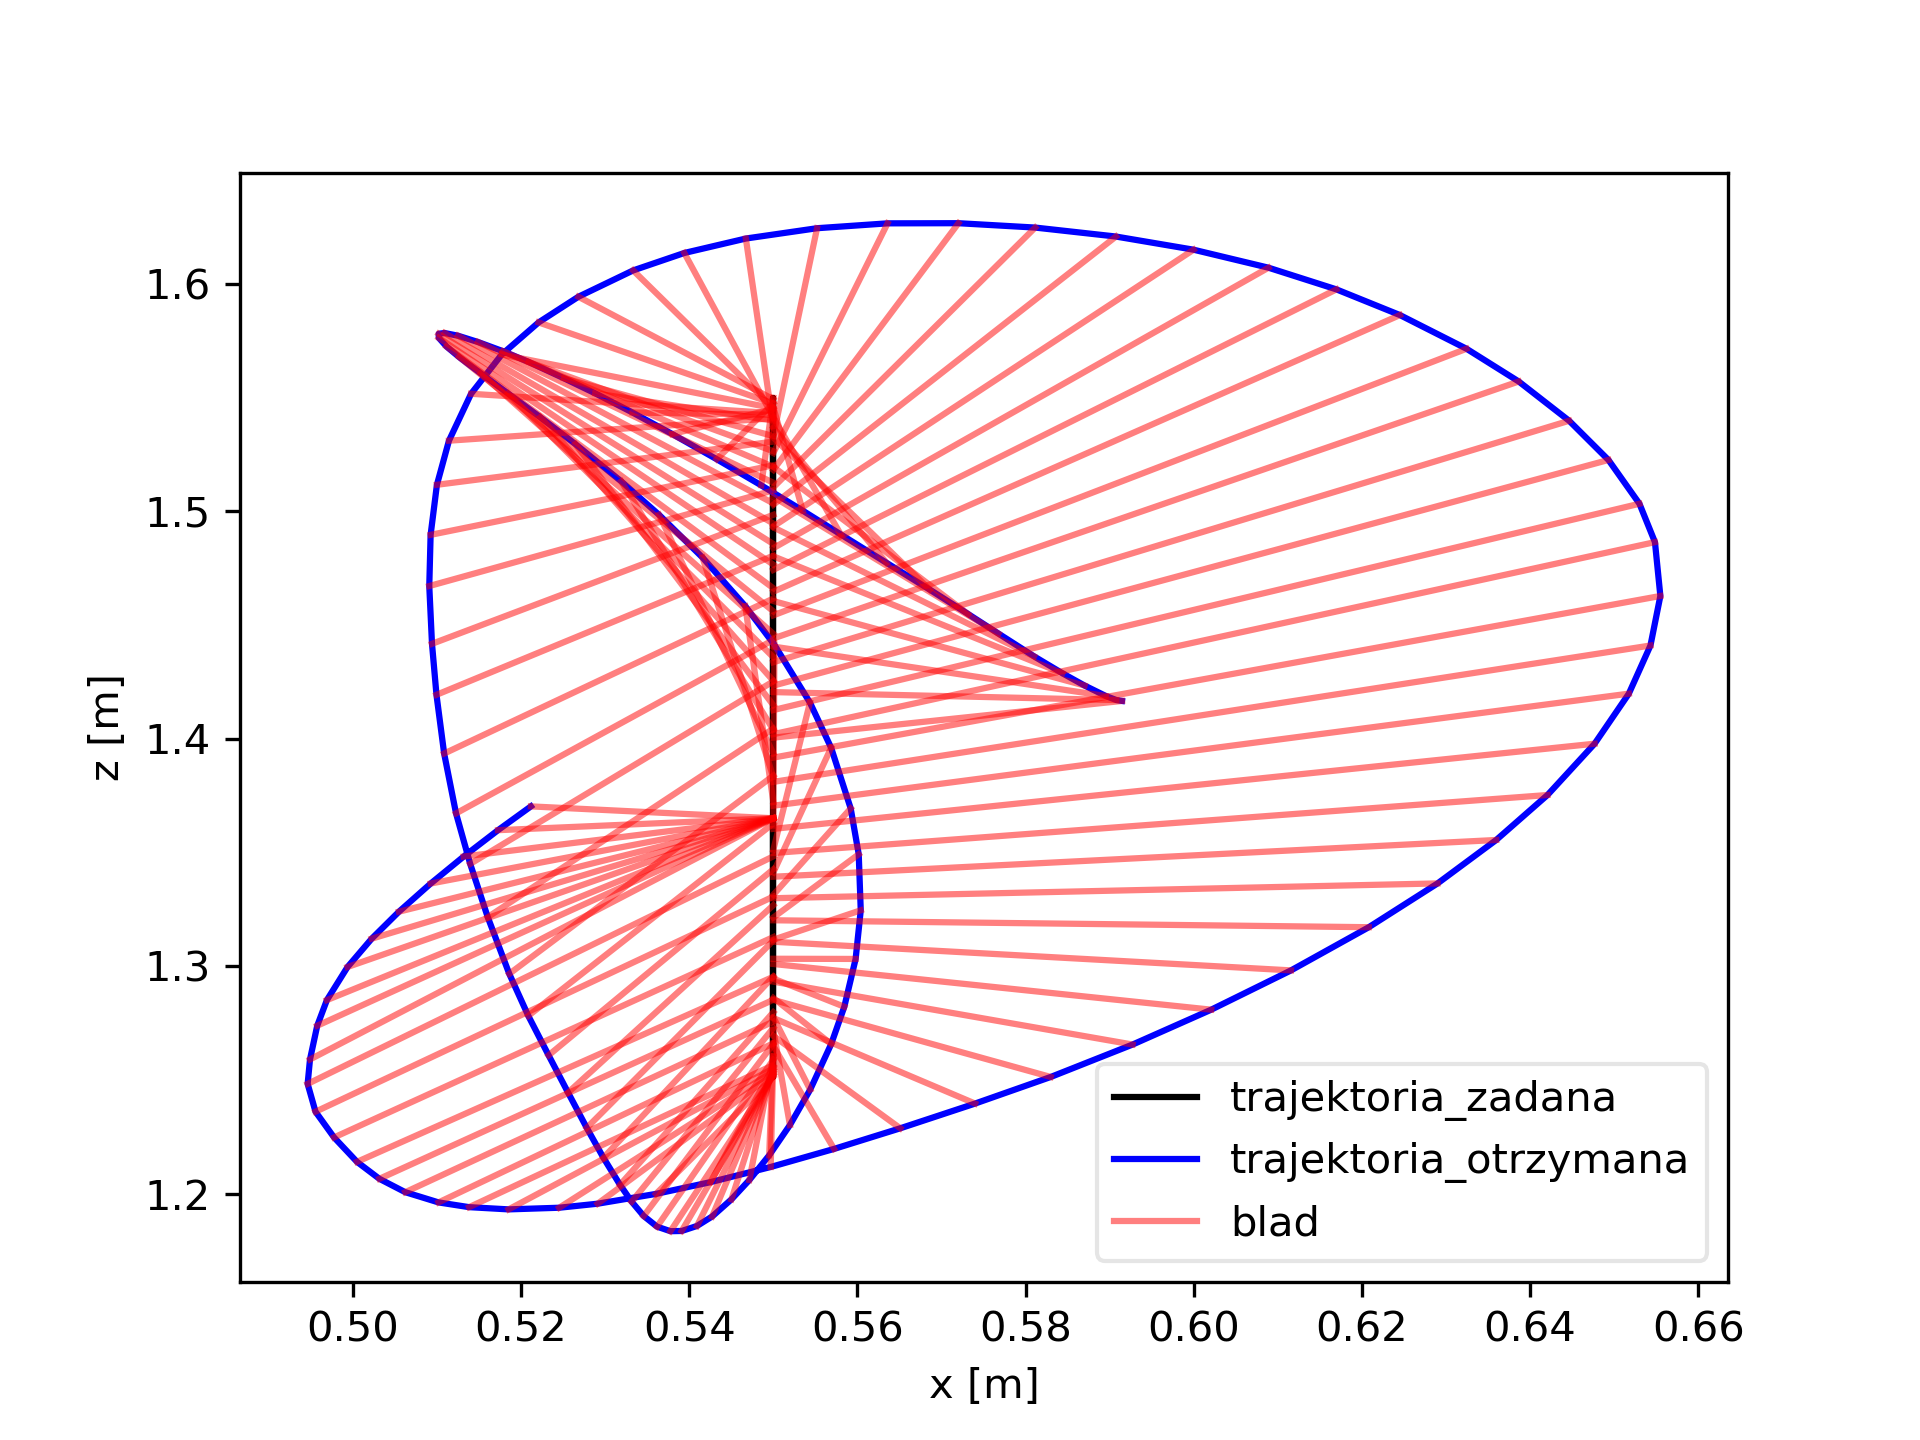
\includegraphics[width=.45\textwidth]{../../velma/przerobione_testy/out/osemka/xz_ate_plot_podnoszenie_miekki_komp_brak.png}
	}
	\caption{Porownanie trajektorii chwytaka w osiach $X$ i $Z$}
	\label{fig:osemka_porow_komp_bok}
\end{figure}

\begin{figure}
	\centering
	\subfigure[Trajektoria z chwycona puszka]{
		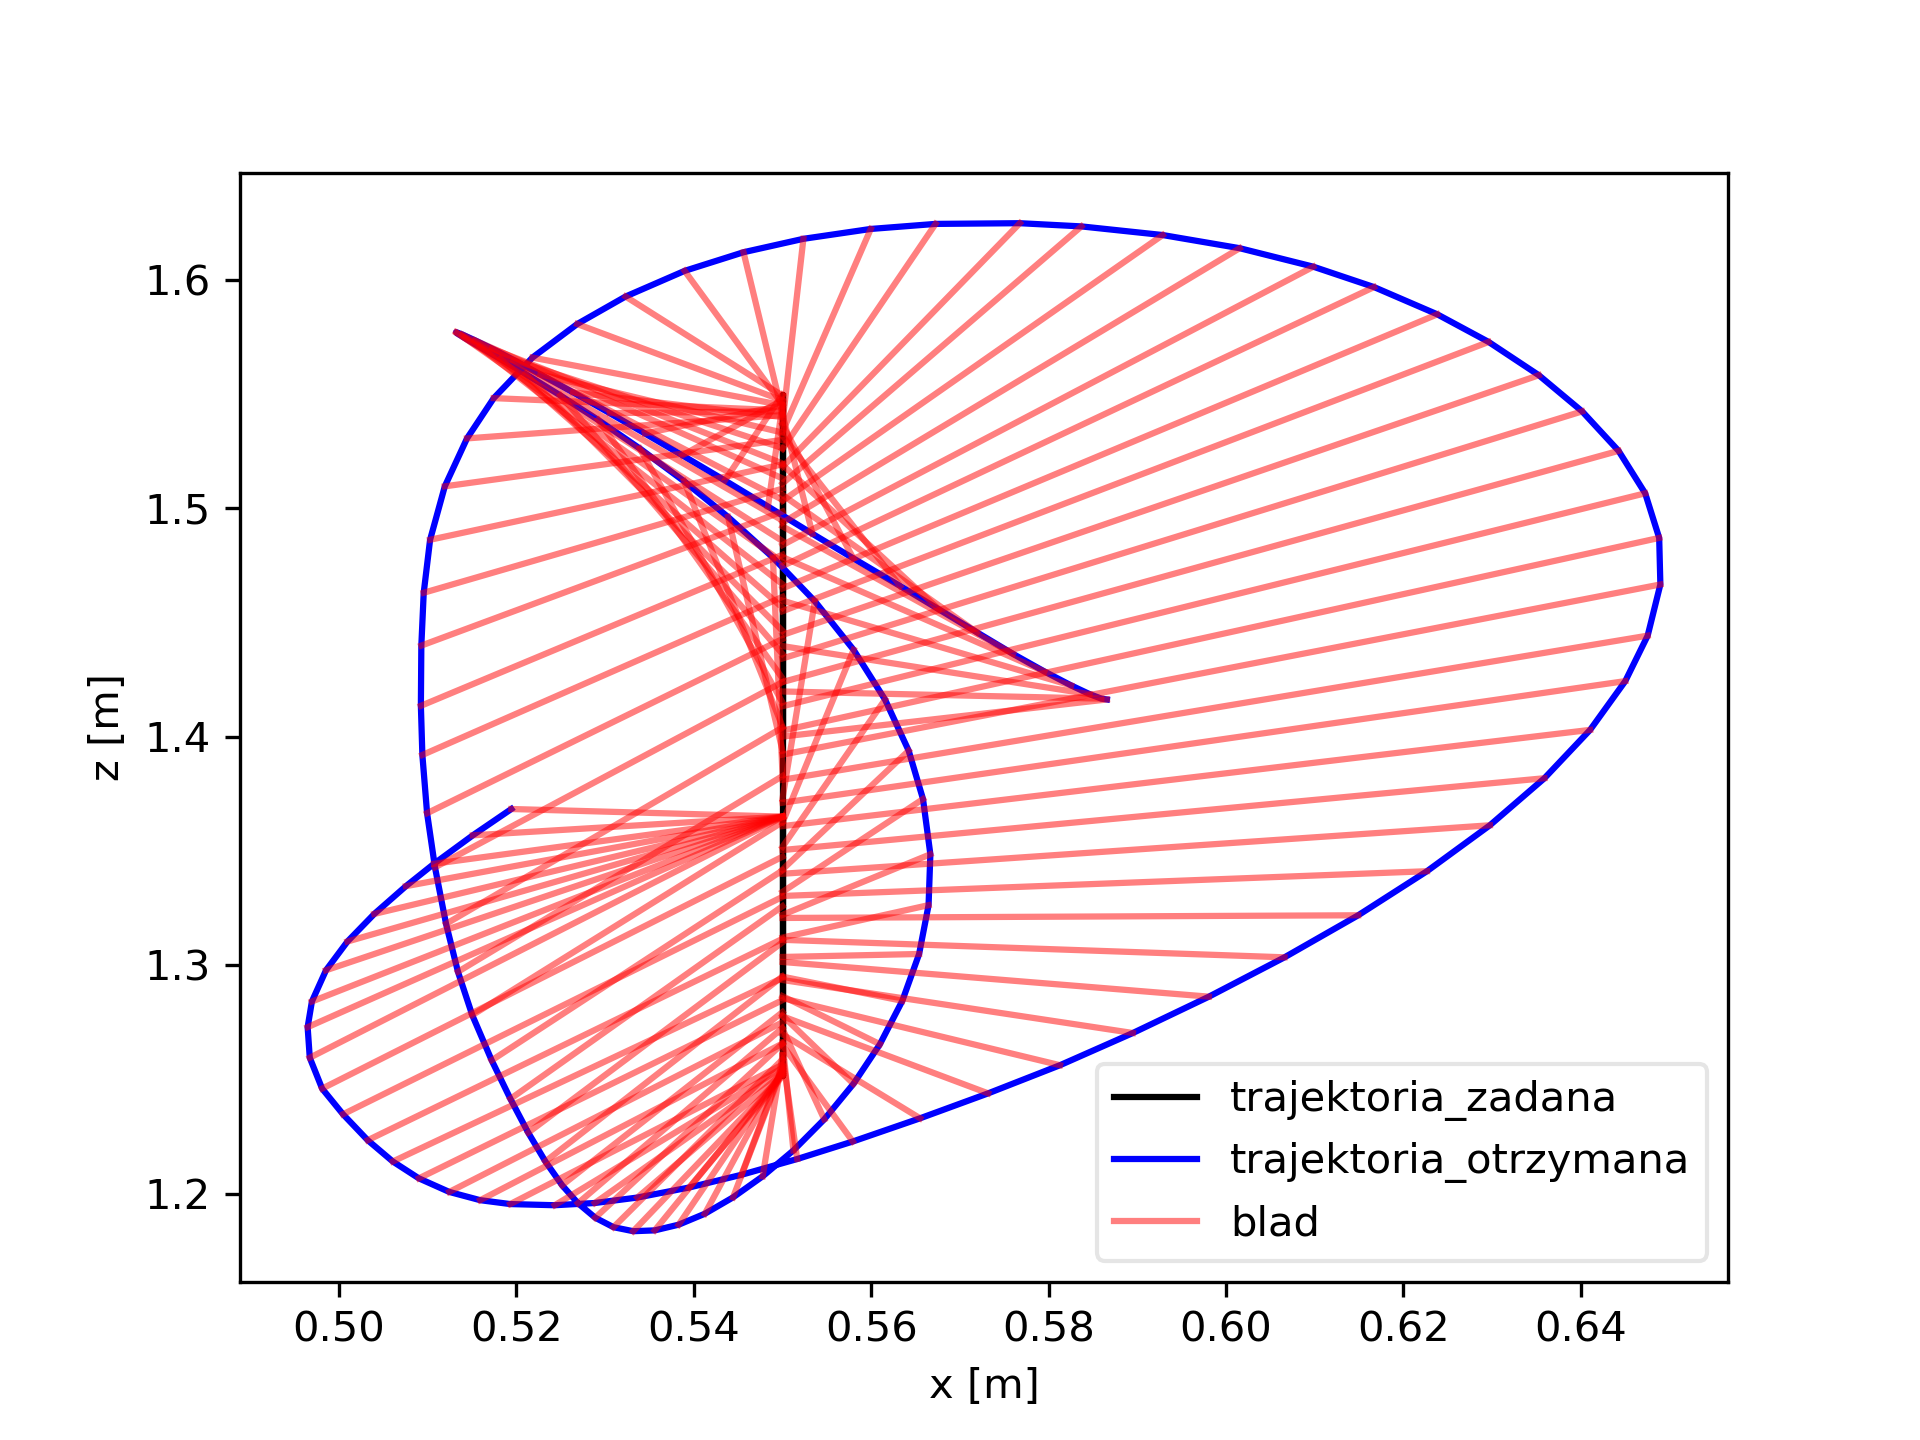
\includegraphics[width=.45\textwidth]{../../velma/przerobione_testy/out/osemka/xz_ate_plot_podnoszenie_miekki_komp_piwo.png}
	}
	\hfill
	\subfigure[Trajektoria z chwycona wiertarka]{
		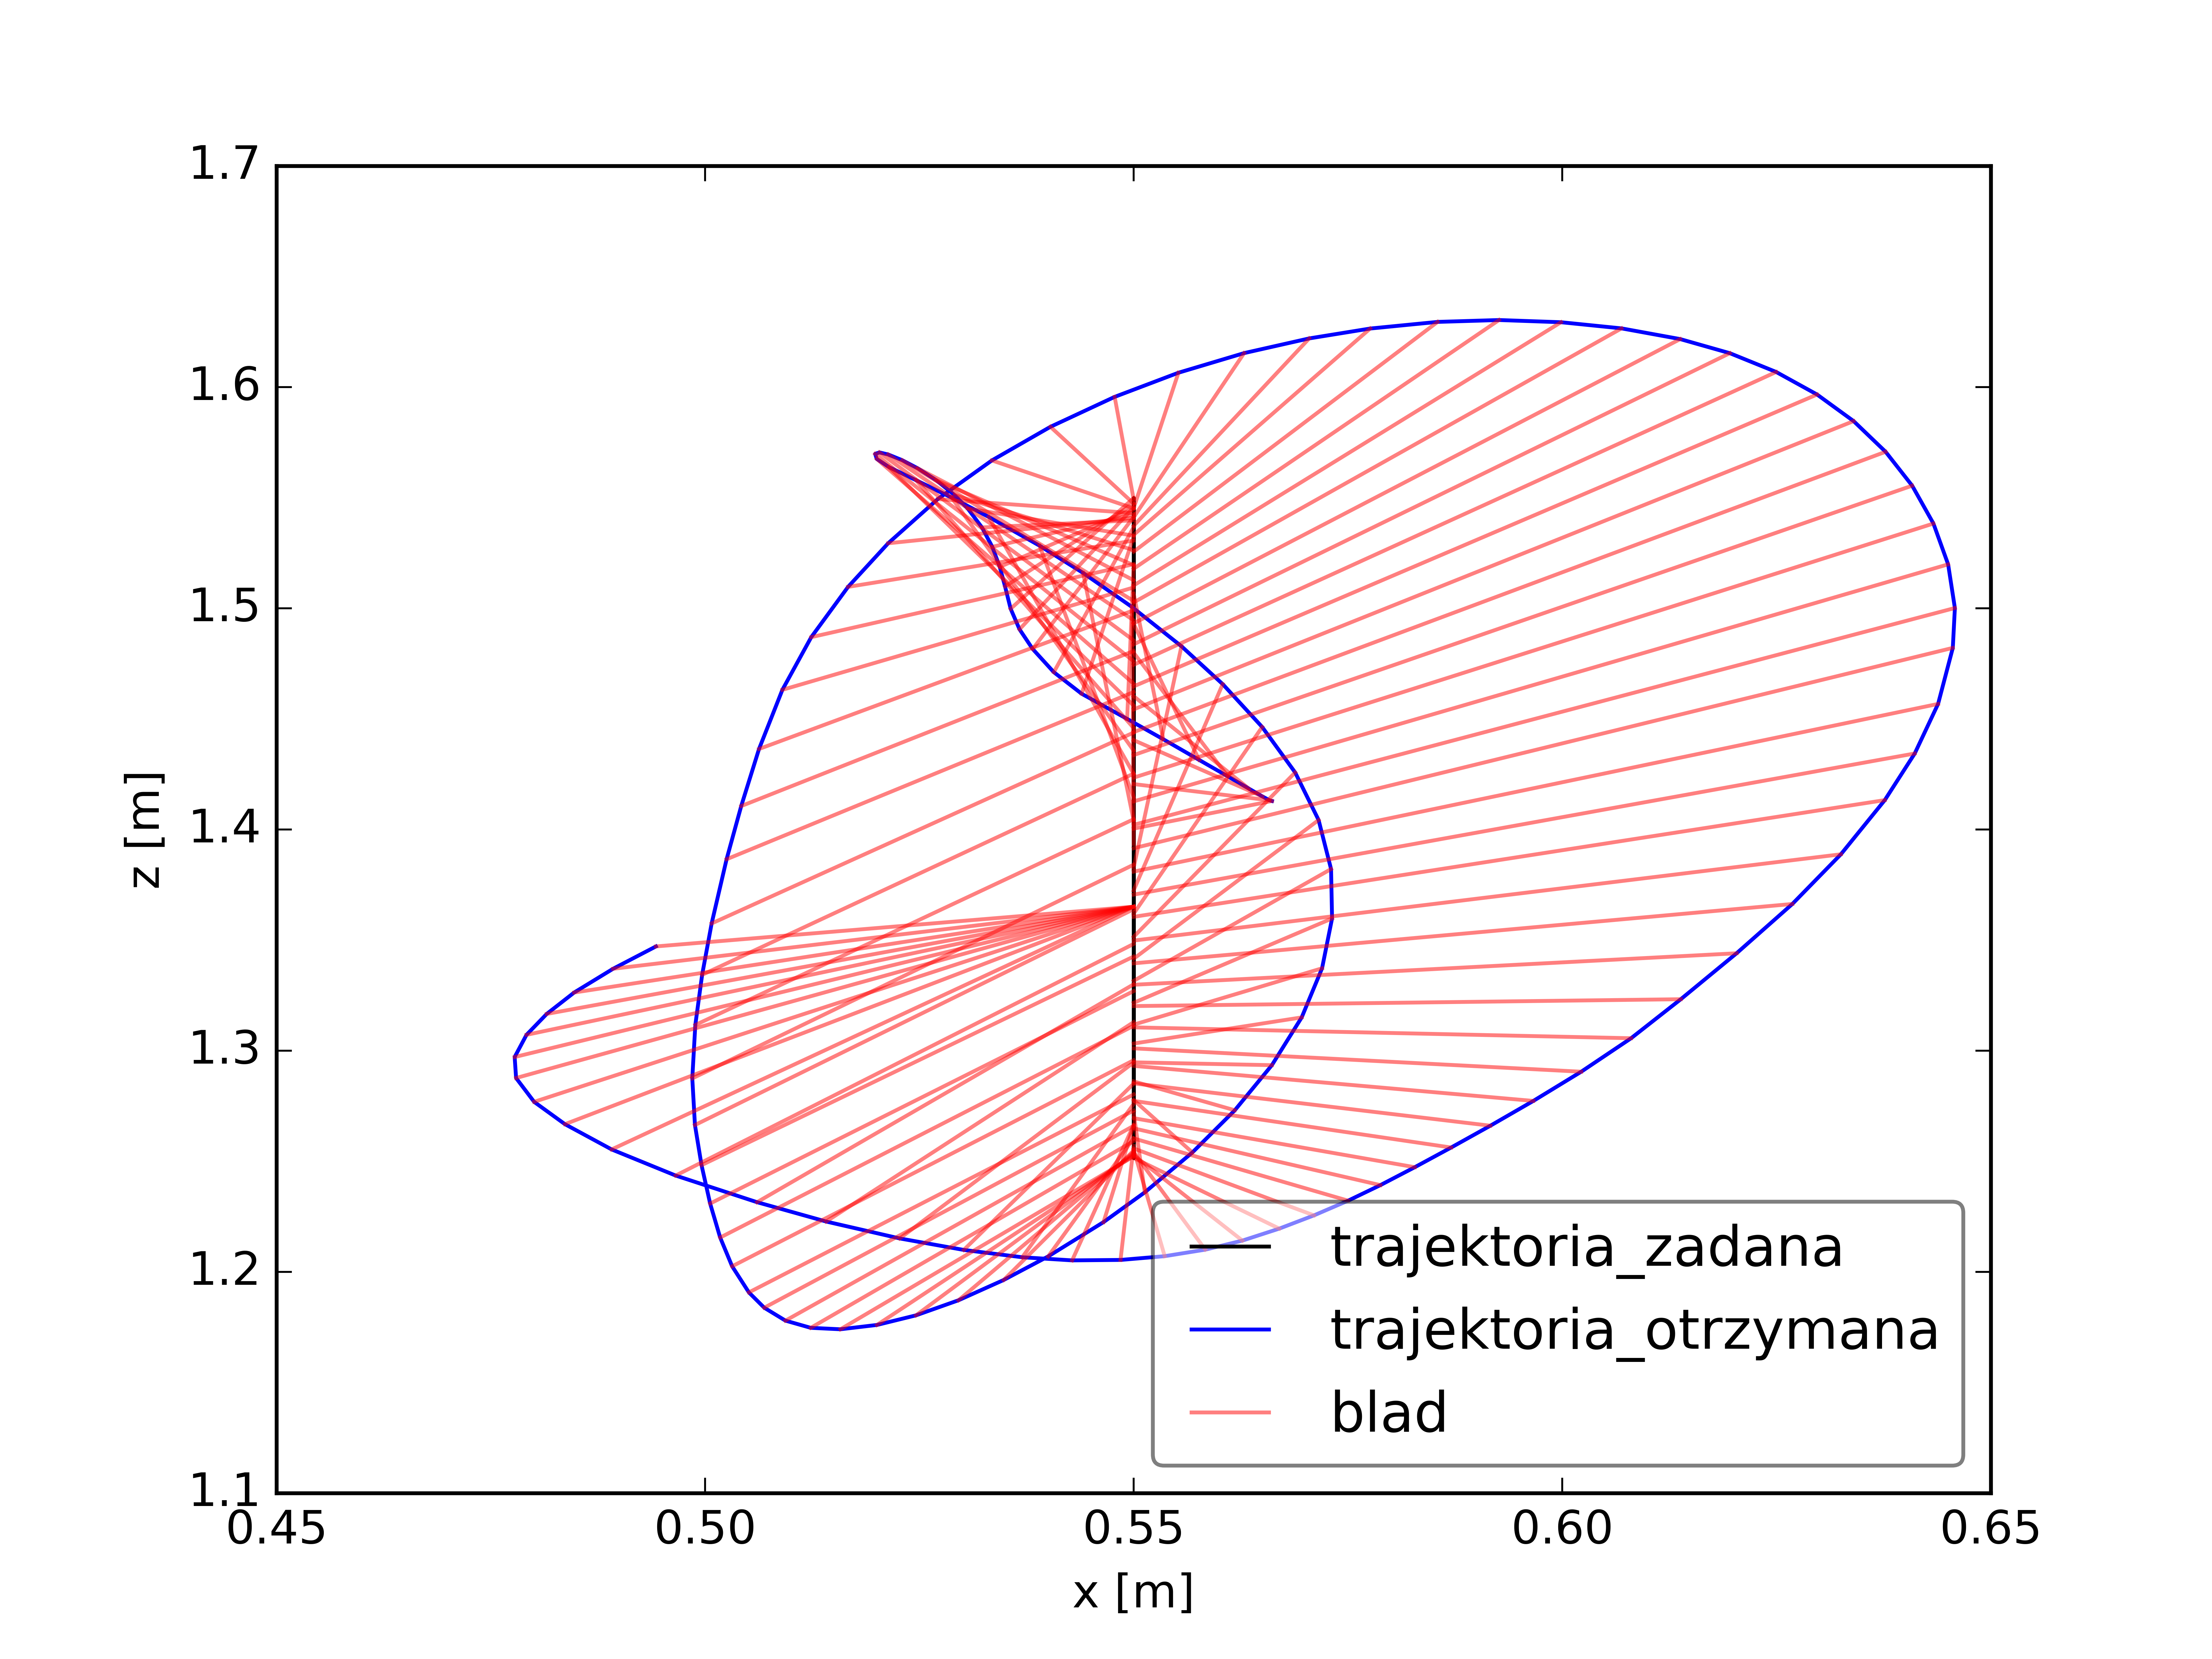
\includegraphics[width=.45\textwidth]{../../velma/przerobione_testy/out/osemka/xz_ate_plot_podnoszenie_miekki_komp_wiertarka.png}
	}
	\caption{Porownanie trajektorii chwytaka w osiach $X$ i $Z$}
	\label{fig:osemka_porow_przedm_bok}
\end{figure}

\begin{figure}
	\centering
	\subfigure[Rzut na wprost]{
		\label{fig:osemka_porow_zbiorcze_a}
		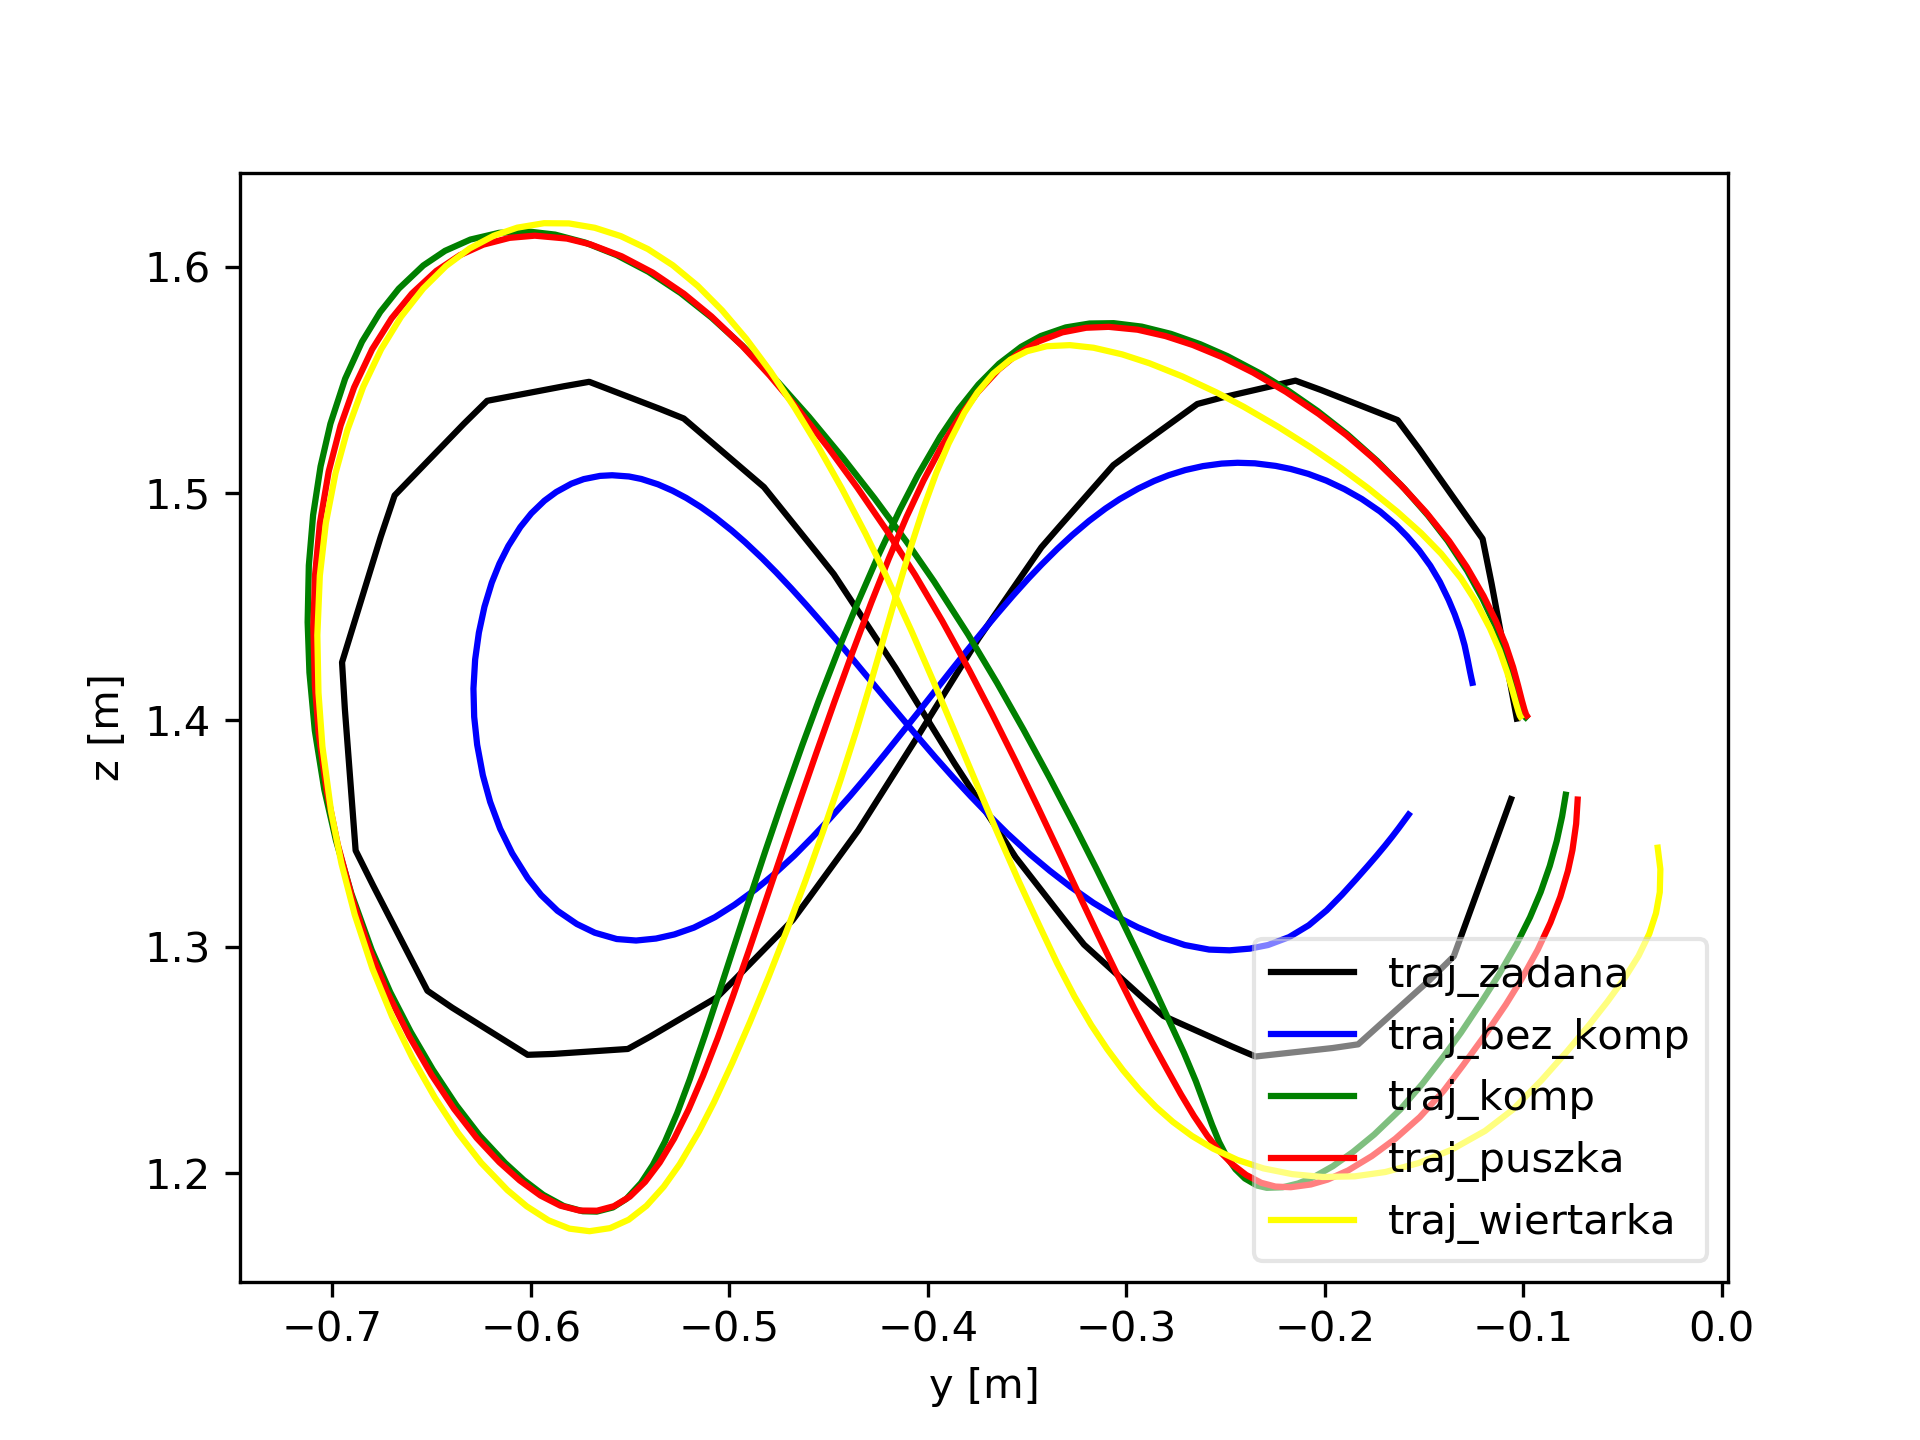
\includegraphics[width=.45\textwidth]{../../velma/przerobione_testy/out/osemka/common_yz.png}
	}
	\hfill
	\subfigure[Rzut z boku]{
		\label{fig:osemka_porow_zbiorcze_b}
		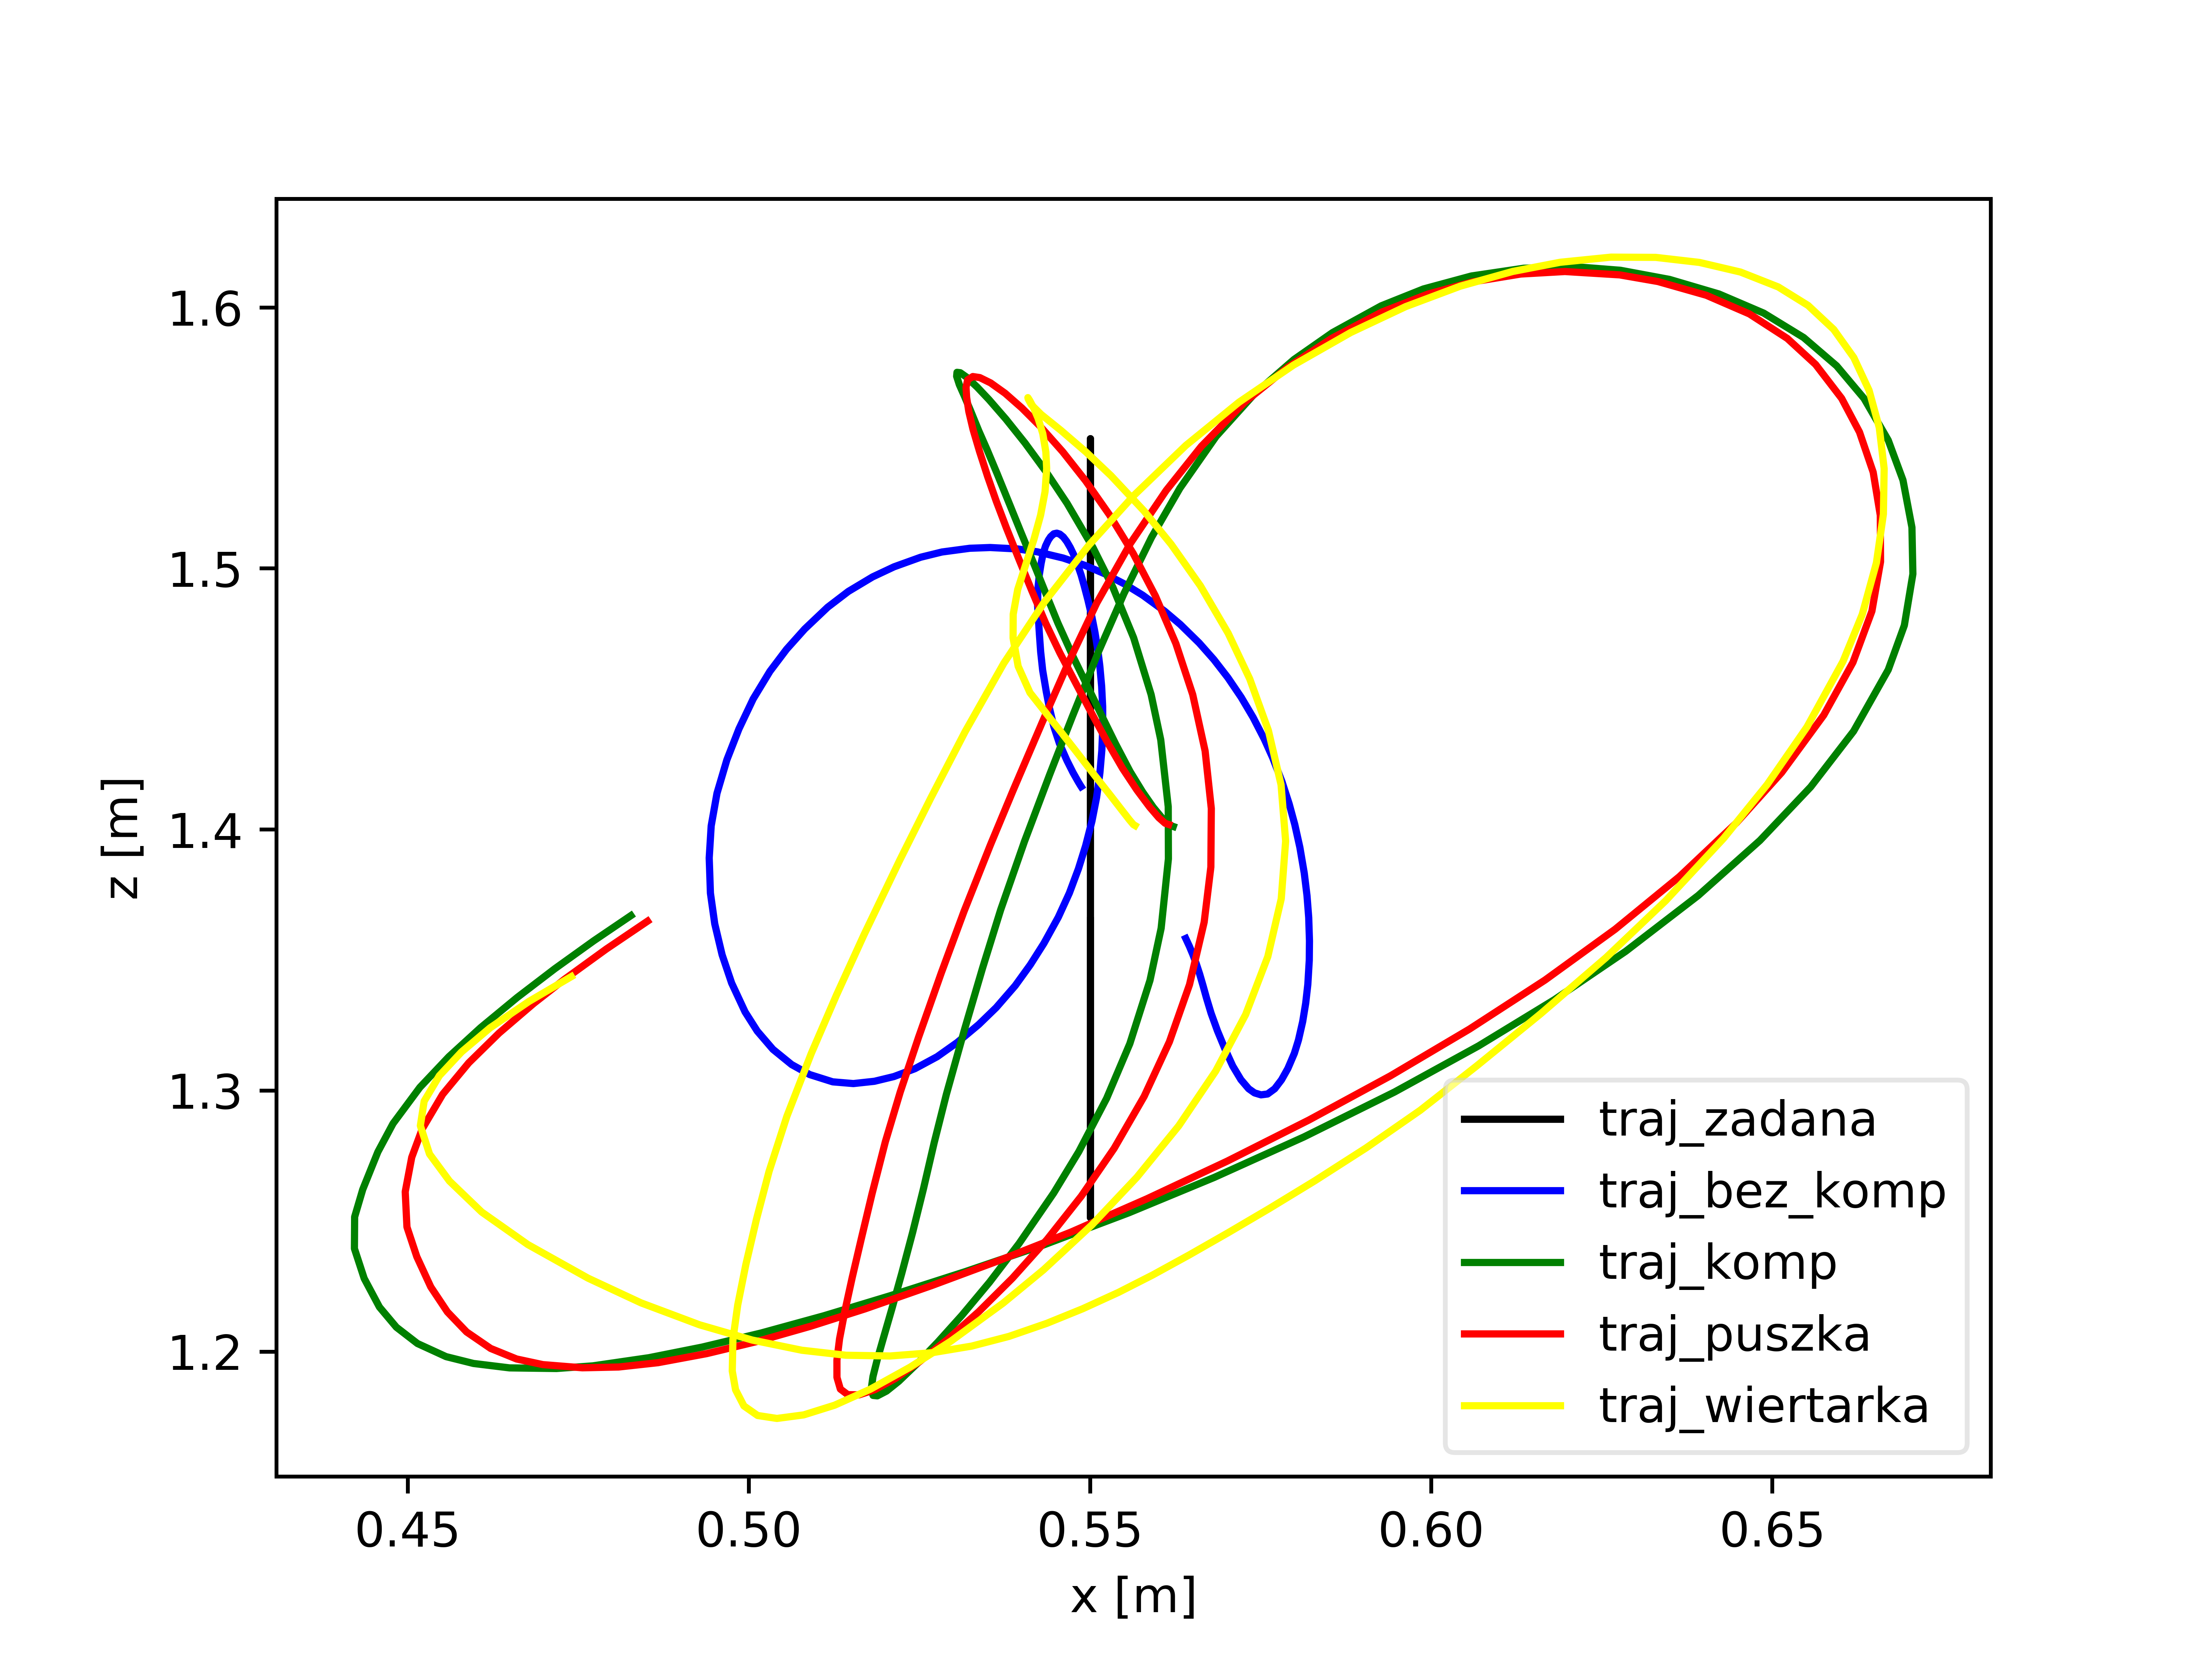
\includegraphics[width=.45\textwidth]{../../velma/przerobione_testy/out/osemka/common_xz.png}
	}
	\caption{Porowanie wszystkich trajektorii bez zaznaczonego bledu.}
	\label{fig:osemka_porow_zbiorcze}
\end{figure}

\subsection{Ruch w bok}

Eksperyment ma przetestowac zachowanie algorytmu kompensacji przy ruchu koncowki w bok. Trajektoria ruchu w rzucie na wprost ruchu zostala zaprezentowana na rys. \ref{fig:w_bok_miekki_porow_komp}, \ref{fig:w_bok_miekki_porow_przedm} i \ref{fig:w_bok_miekki_porow_zbiorcze_a}. 
% Trajektoria widoczna z boku (w osiach $X$ oraz $Z$) zostala zaprezentowana na rys. \ref{fig:w_bok_miekki_porow_komp_bok}, \ref{fig:w_bok_miekki_porow_przedm_bok} i \ref{fig:w_bok_miekki_porow_zbiorcze_b}.
\begin{figure}[h]
	\centering
	\subfigure[Os $X$]{
		\label{fig:w_bok_miekki_ax}
		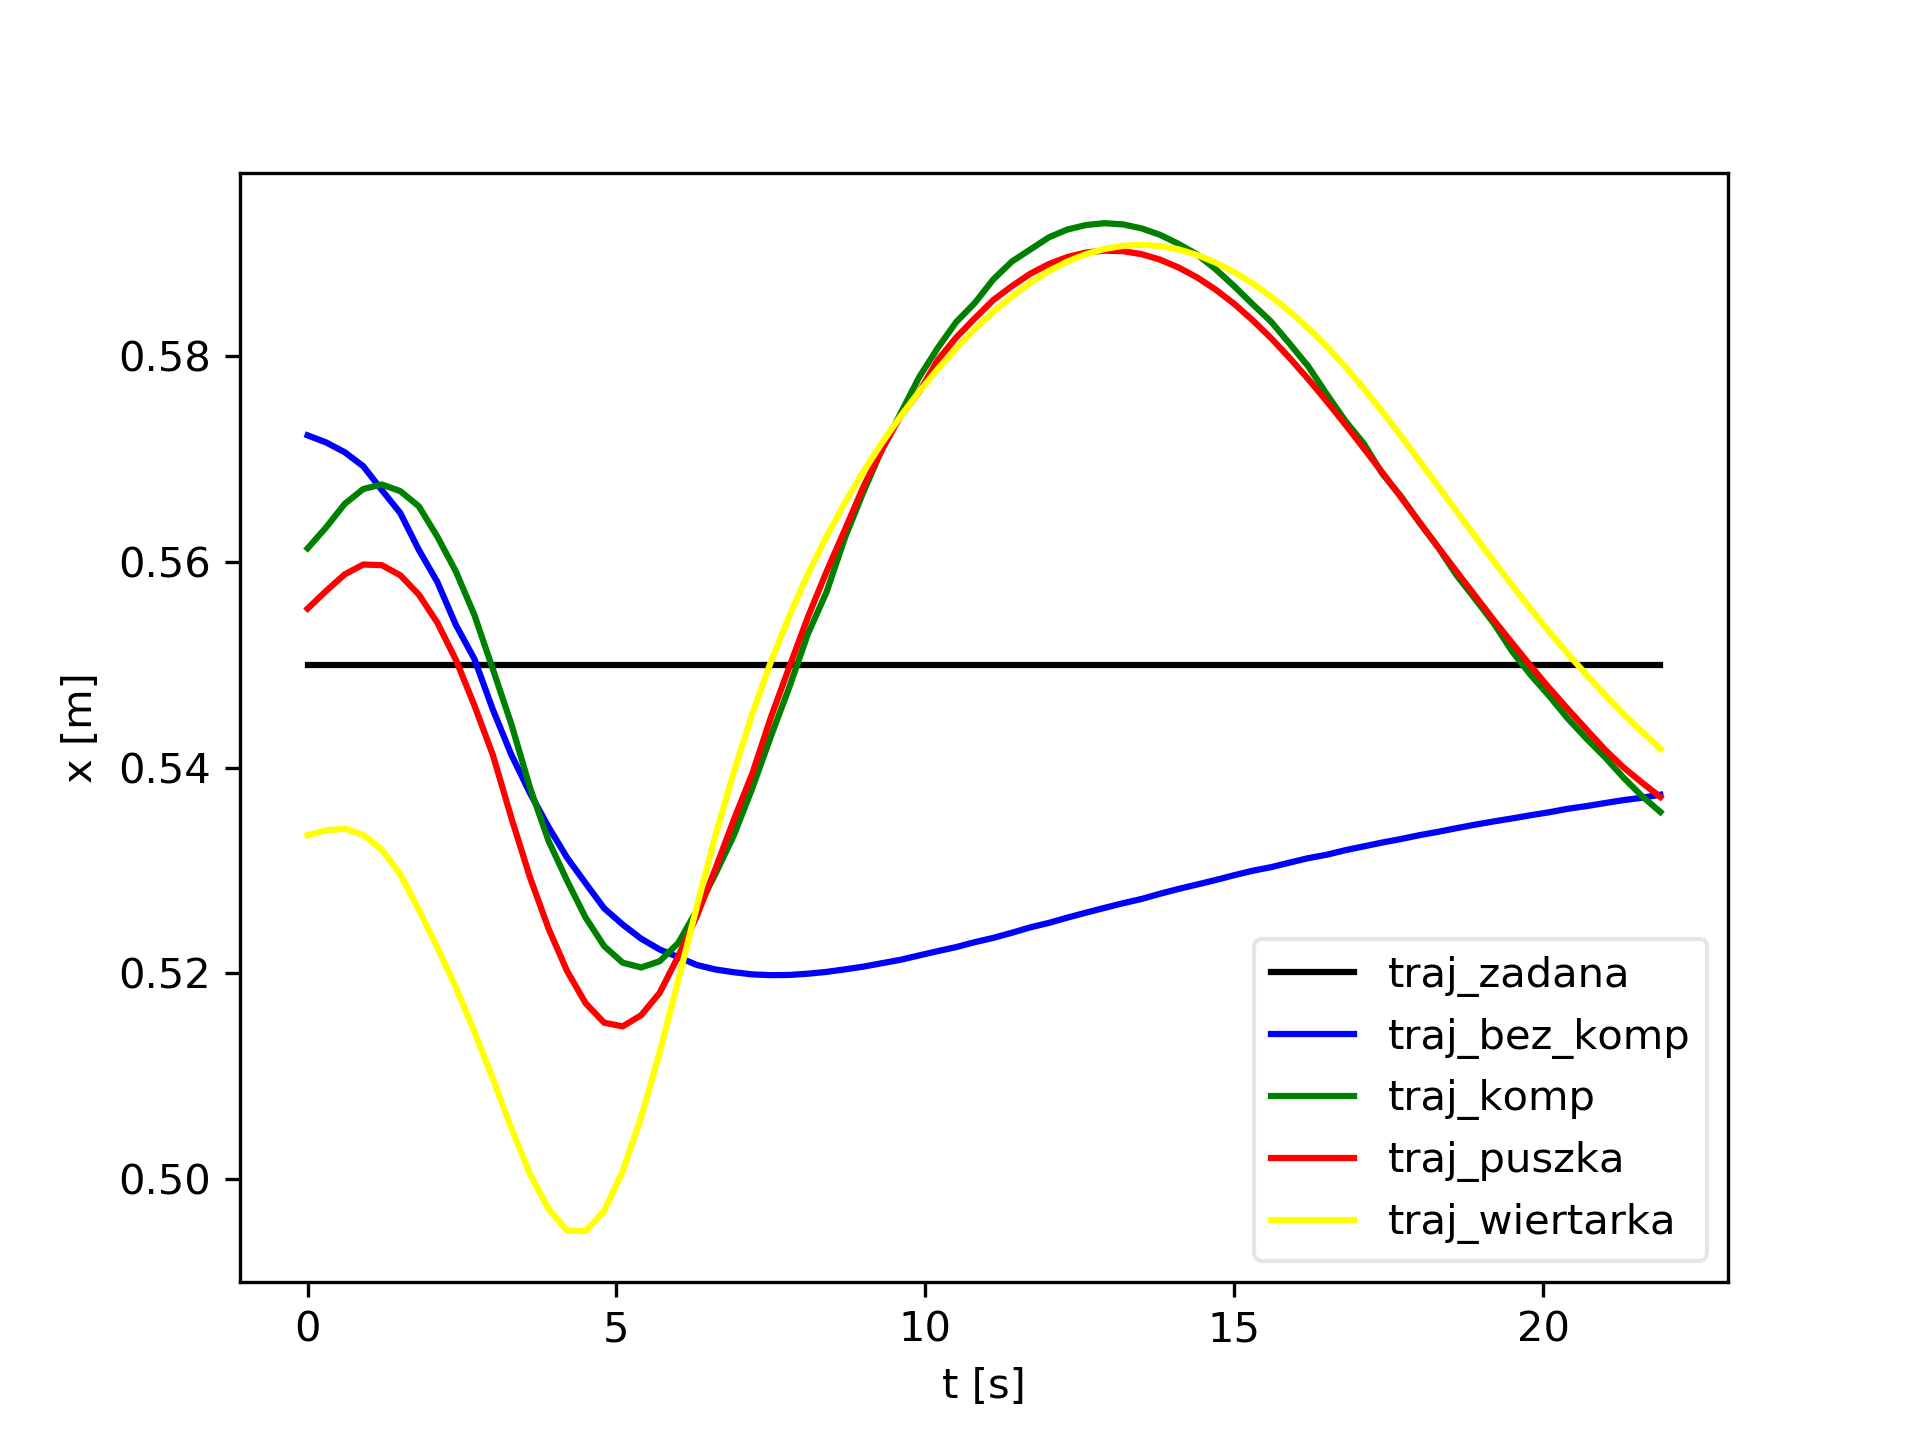
\includegraphics[width=.45\textwidth]{../../velma/przerobione_testy/out/w_bok_miekki/common_ax.png}
	}
	\hfill
	\subfigure[Os $Y$]{
		\label{fig:w_bok_miekki_ay}
		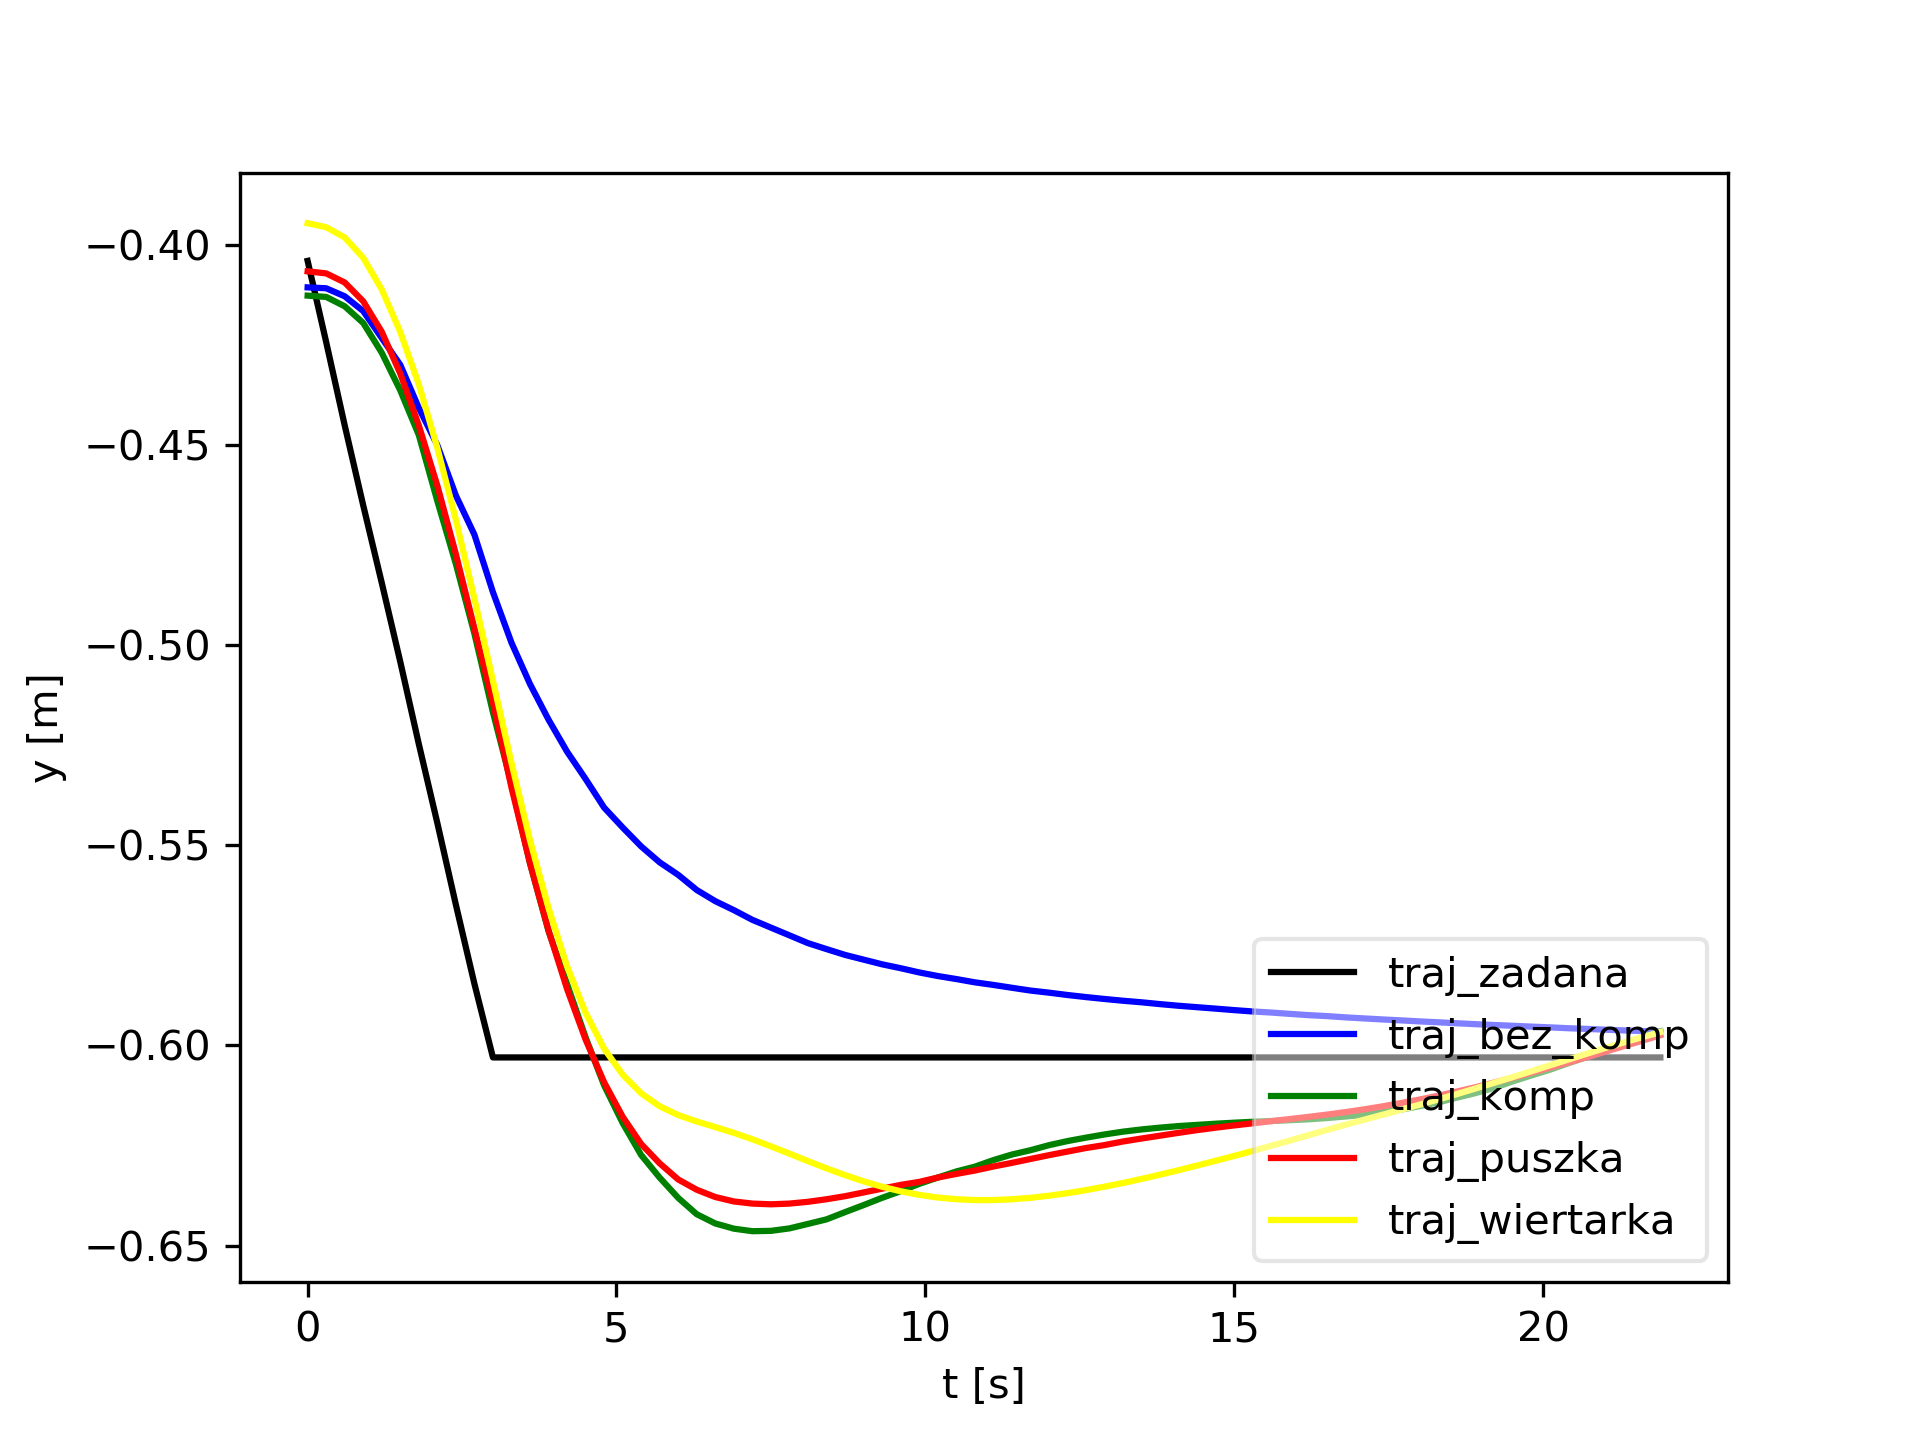
\includegraphics[width=.45\textwidth]{../../velma/przerobione_testy/out/w_bok_miekki/common_ay.png}
	}
	
	\hfill
	\subfigure[Os $Z$]{
		\label{fig:w_bok_miekki_az}
		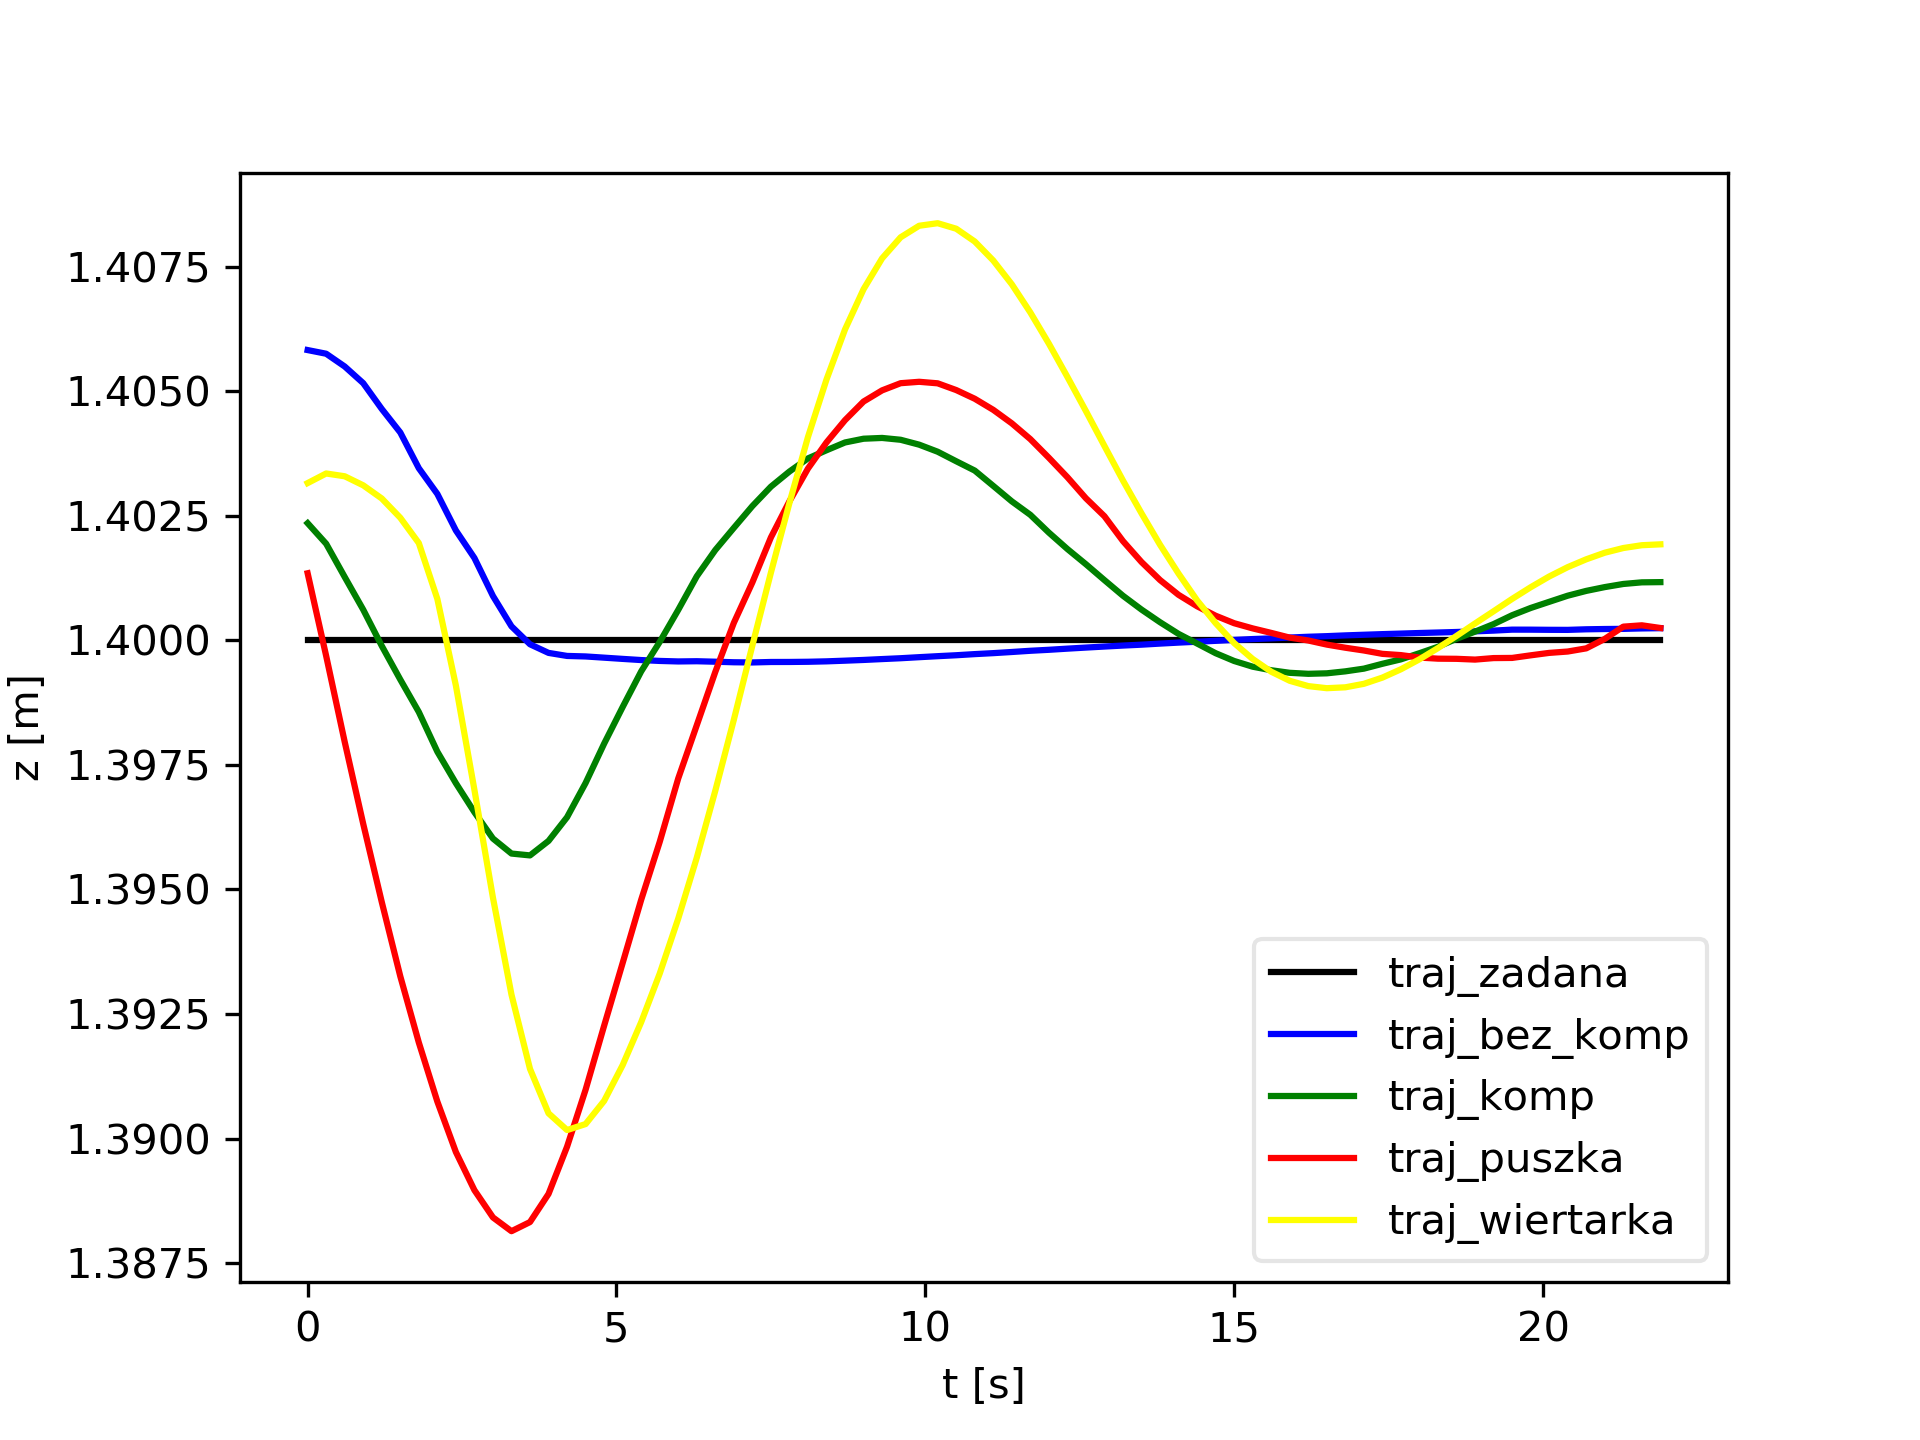
\includegraphics[width=.45\textwidth]{../../velma/przerobione_testy/out/w_bok_miekki/common_az.png}
	}

	\caption{Ruch do gory. Porownanie trajektorii pozycji w zaleznosci od czasu.}
	\label{fig:w_bok_miekki_a}

\end{figure}


\begin{figure}[h]
	\centering
	\subfigure[Kat osi $X$]{
		\label{fig:w_bok_miekki_rotx}
		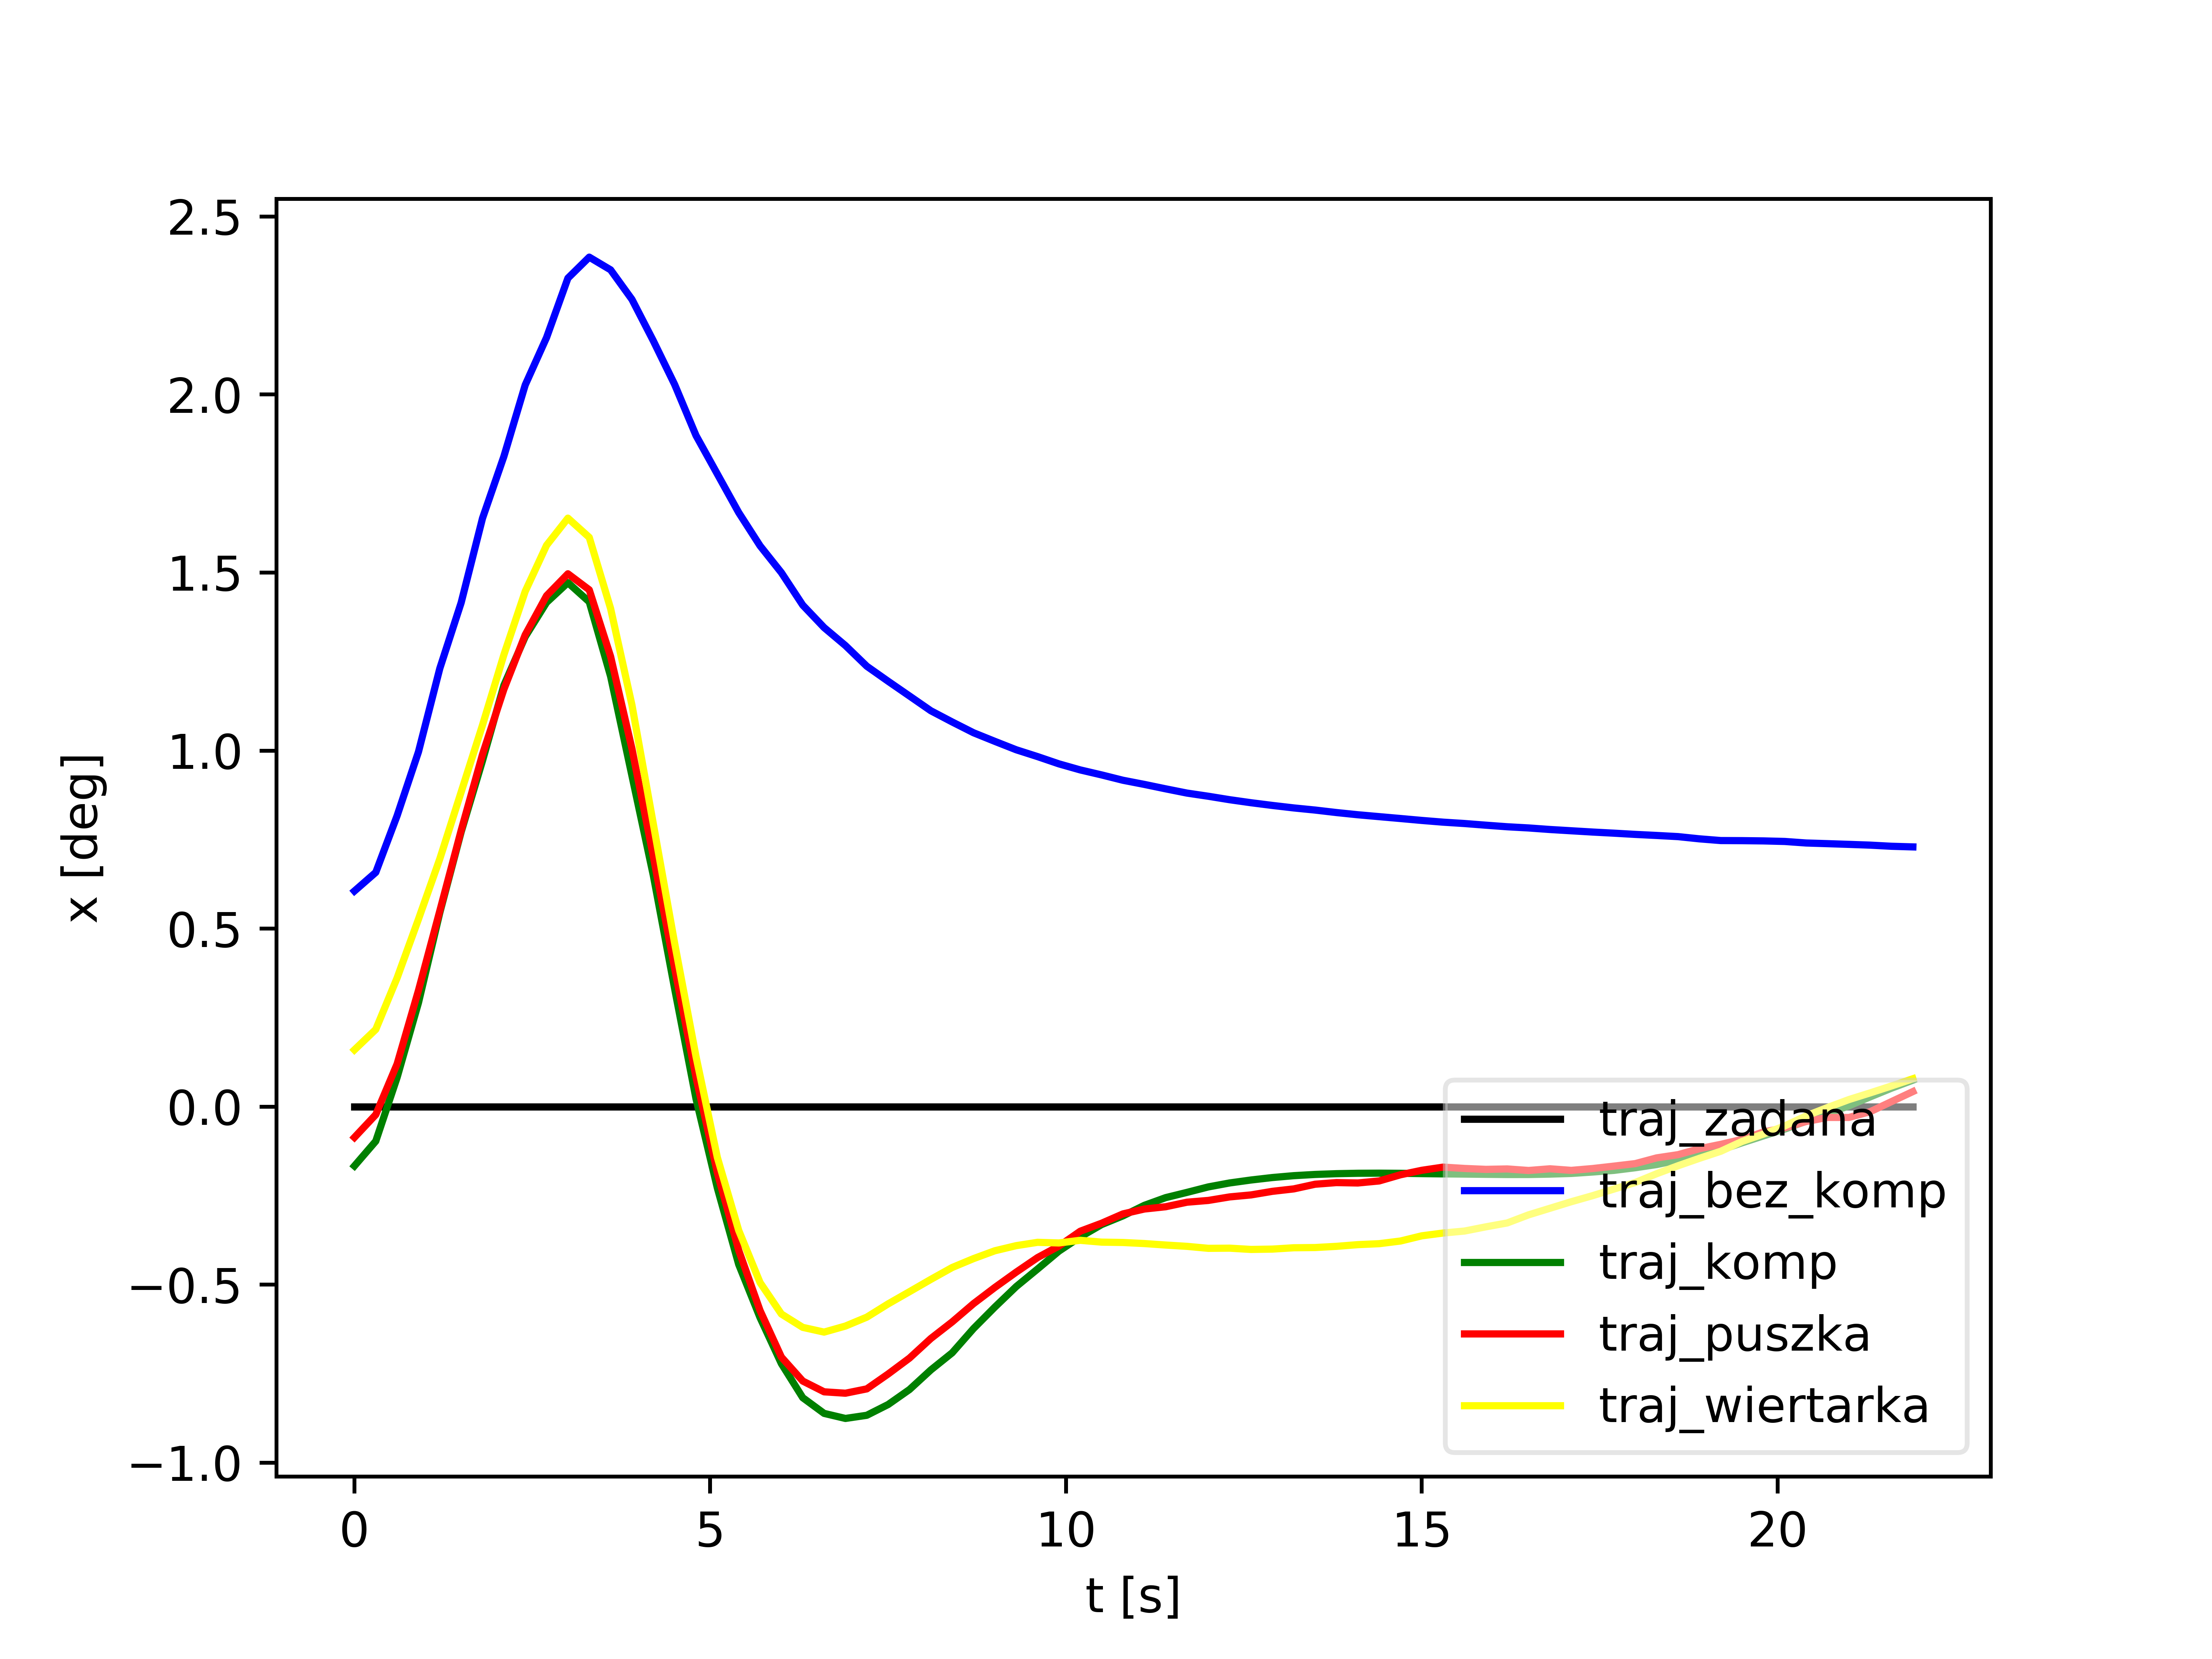
\includegraphics[width=.45\textwidth]{../../velma/przerobione_testy/out/w_bok_miekki/common_rotx.png}
	}
	\hfill
	\subfigure[Kat osi $Y$]{
		\label{fig:w_bok_miekki_roty}
		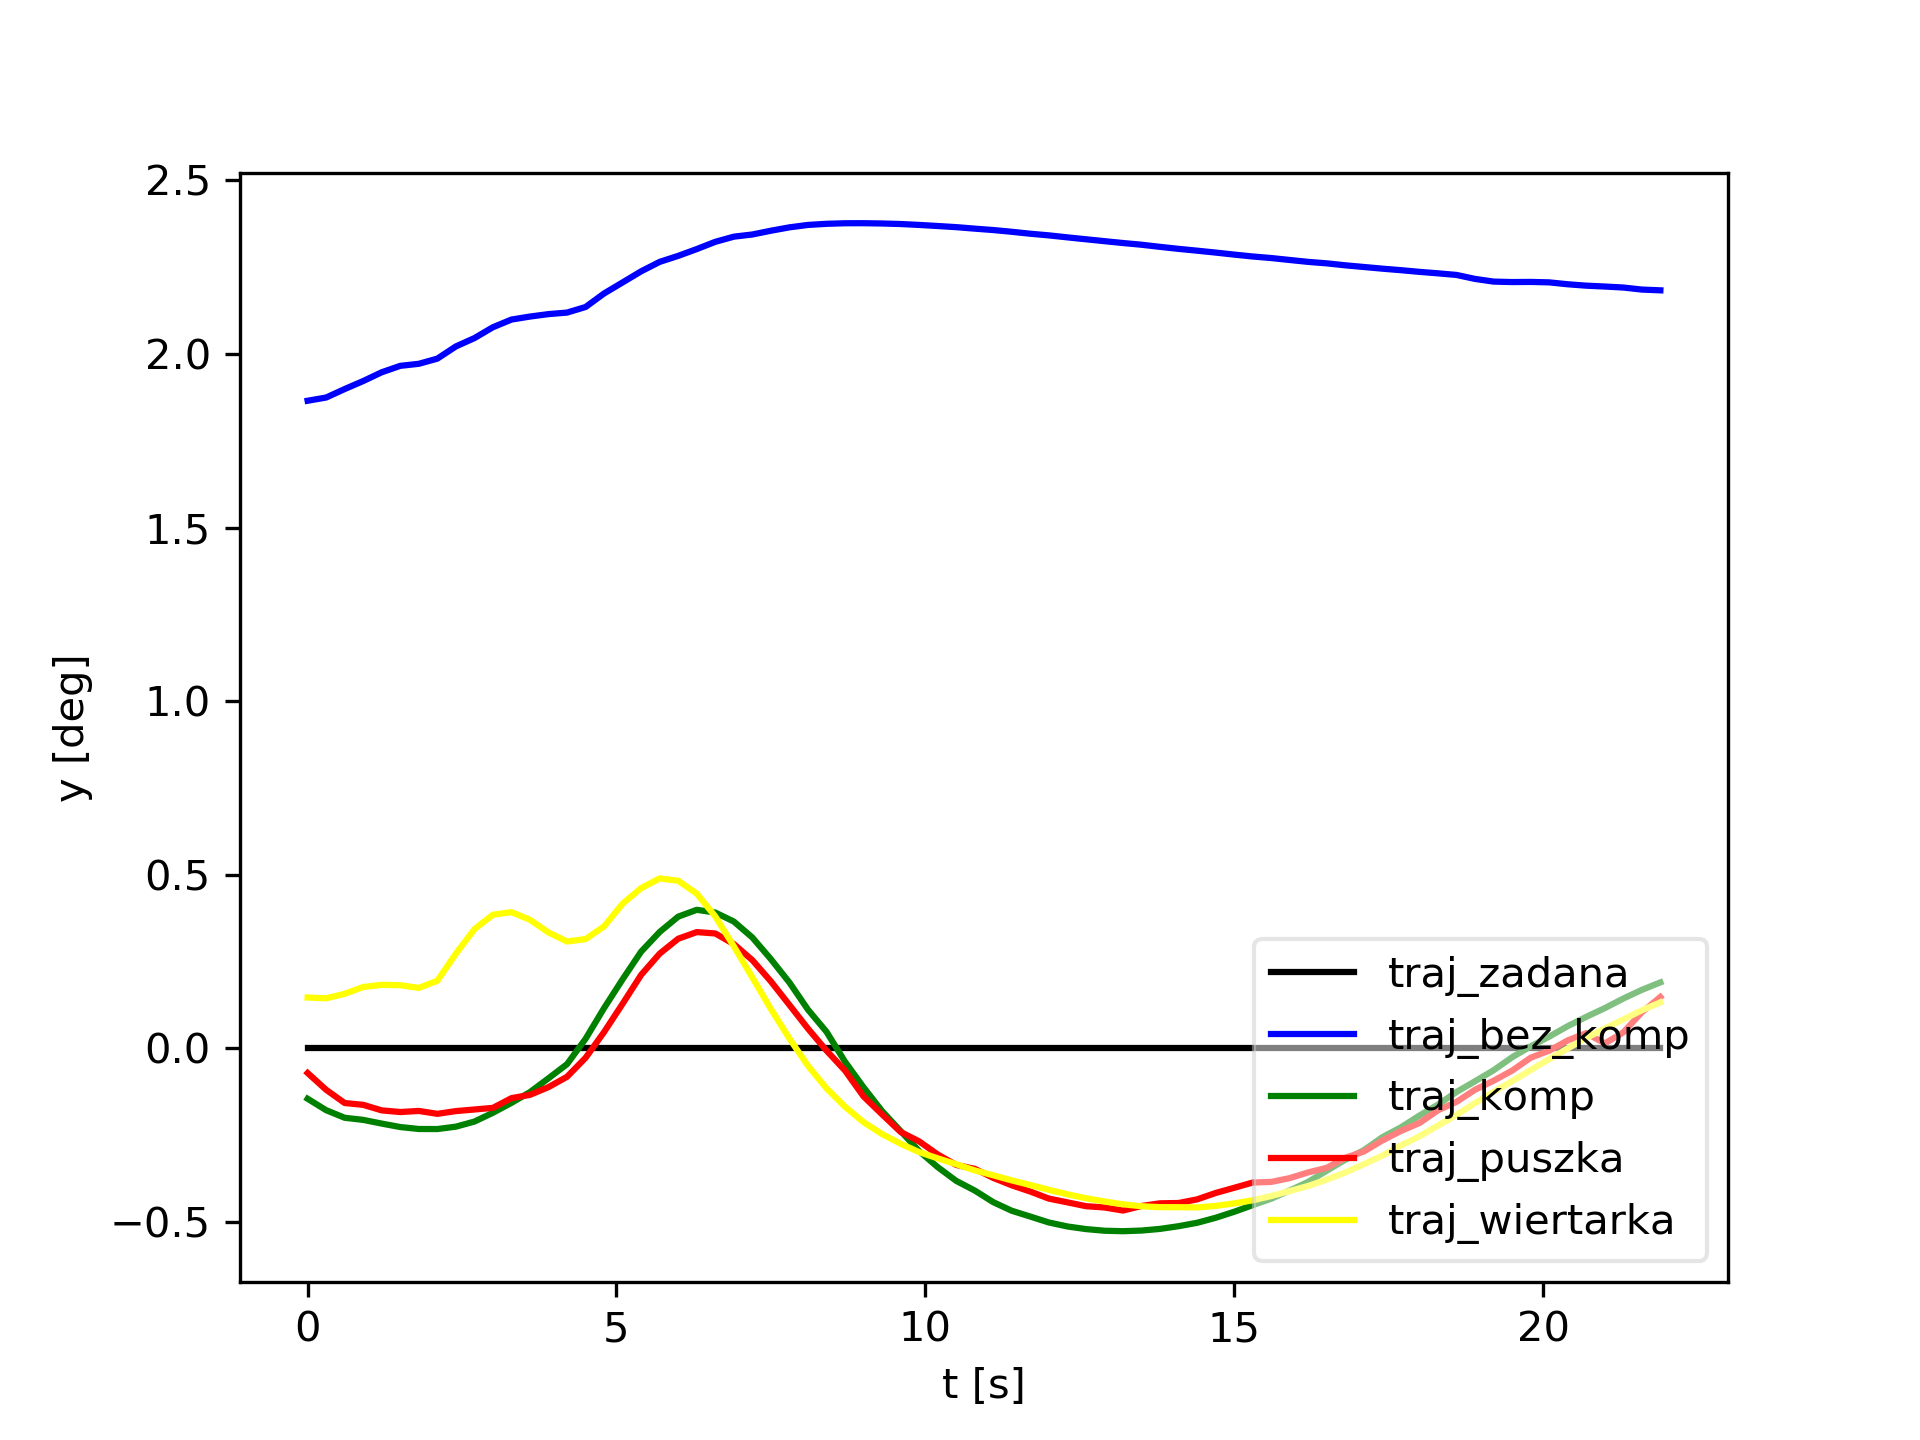
\includegraphics[width=.45\textwidth]{../../velma/przerobione_testy/out/w_bok_miekki/common_roty.png}
	}
	
	\hfill
	\subfigure[Kat osi $Z$]{
		\label{fig:w_bok_miekki_rotz}
		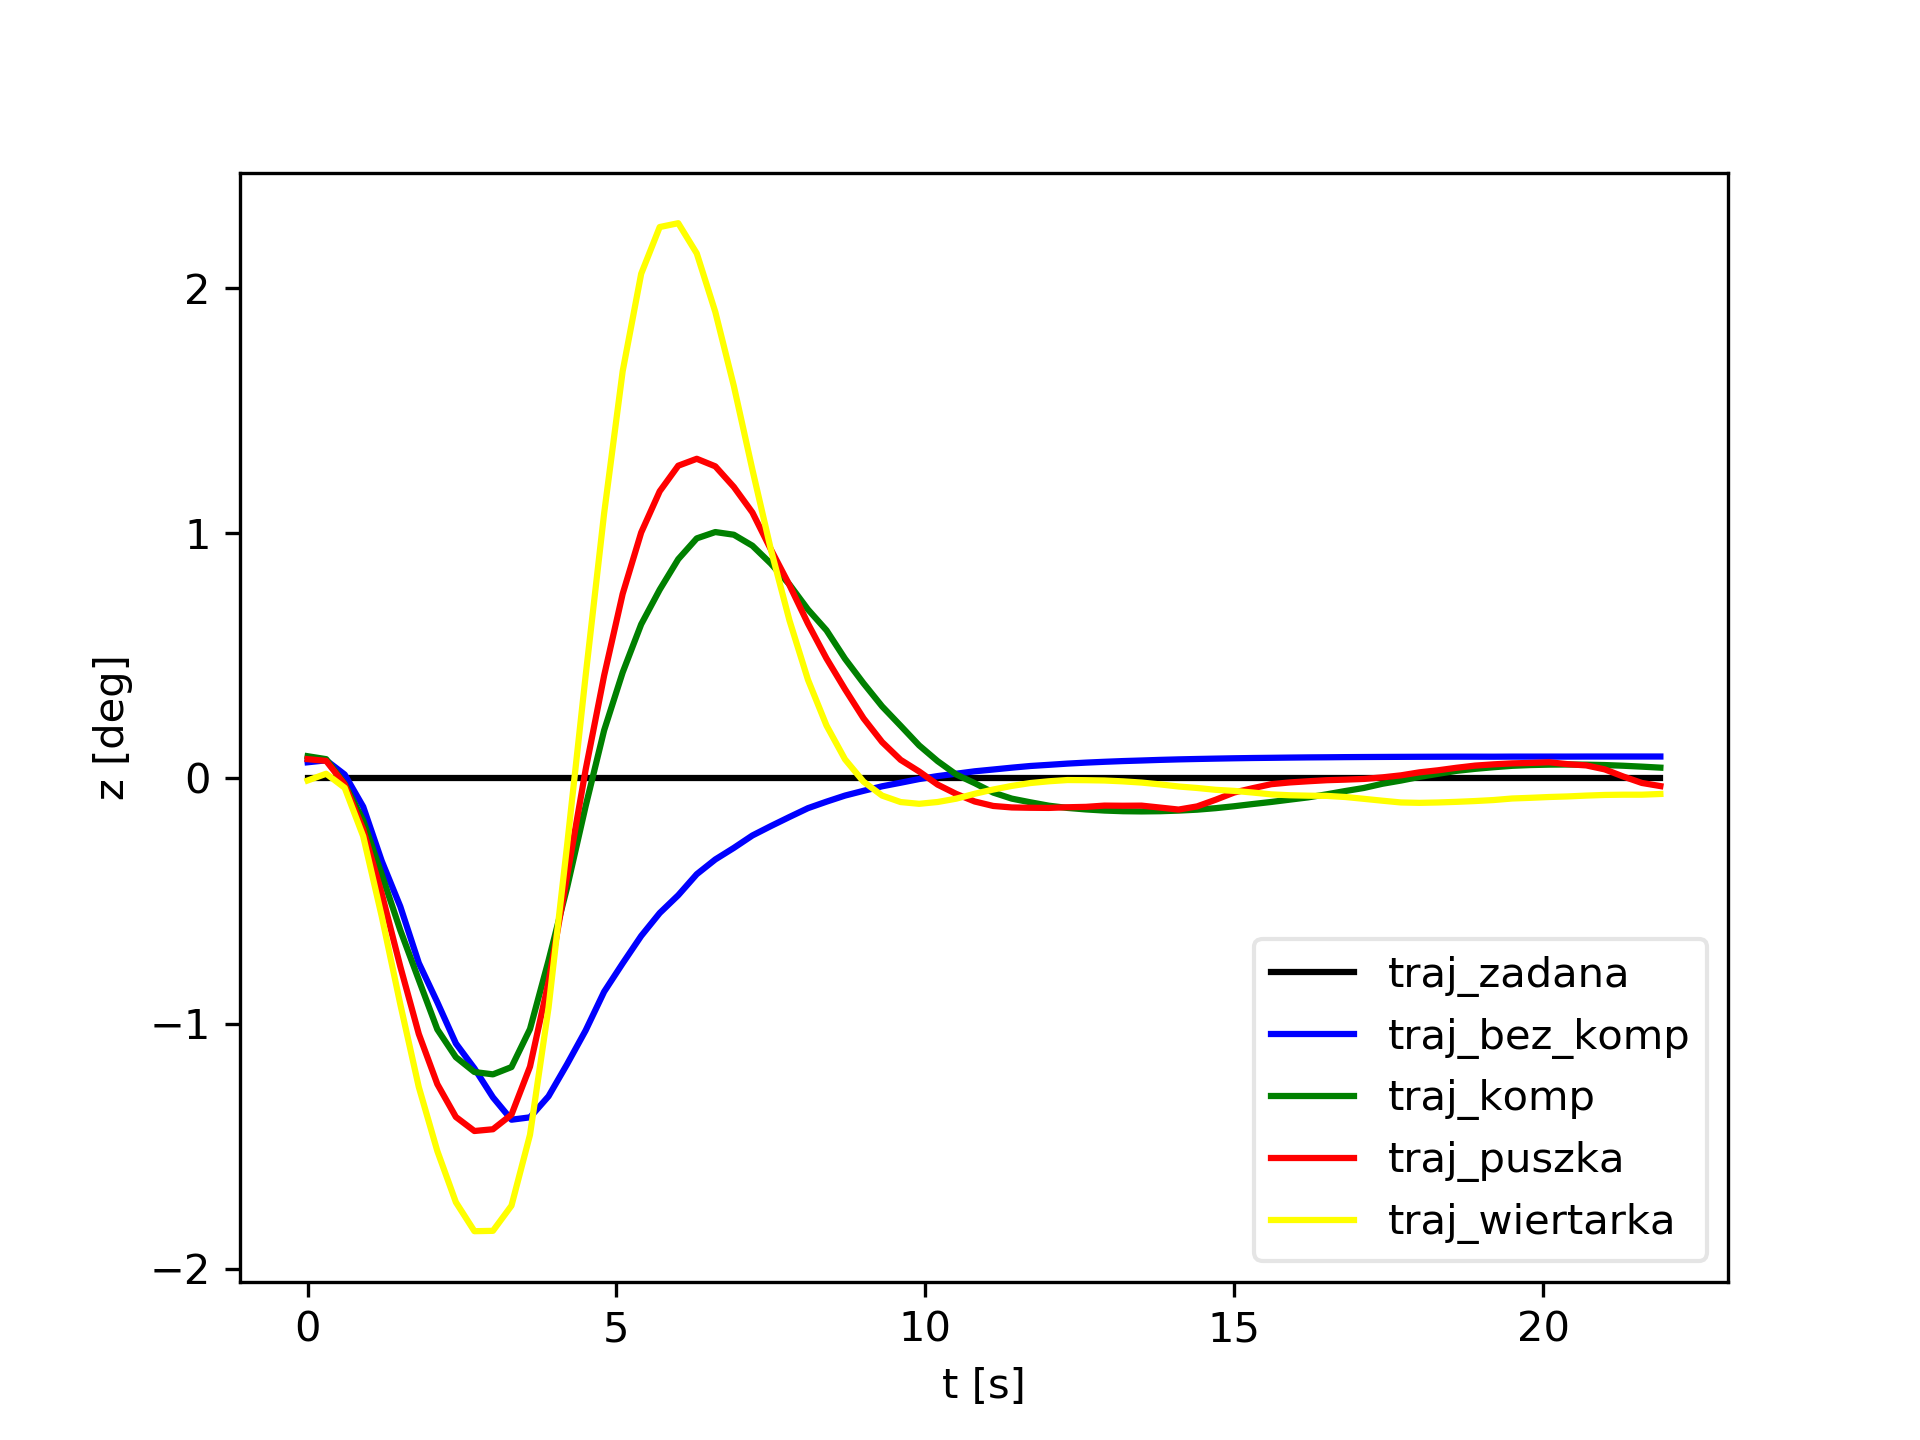
\includegraphics[width=.45\textwidth]{../../velma/przerobione_testy/out/w_bok_miekki/common_rotz.png}
	}

	\caption{Ruch do gory. Porownanie trajektorii katow w notacji Eulera w zaleznosci od czasu.}
	\label{fig:w_bok_miekki_rot}

\end{figure}


\begin{figure}[h]
	\centering
	\subfigure[Brak algorytmu kompensacji]{
		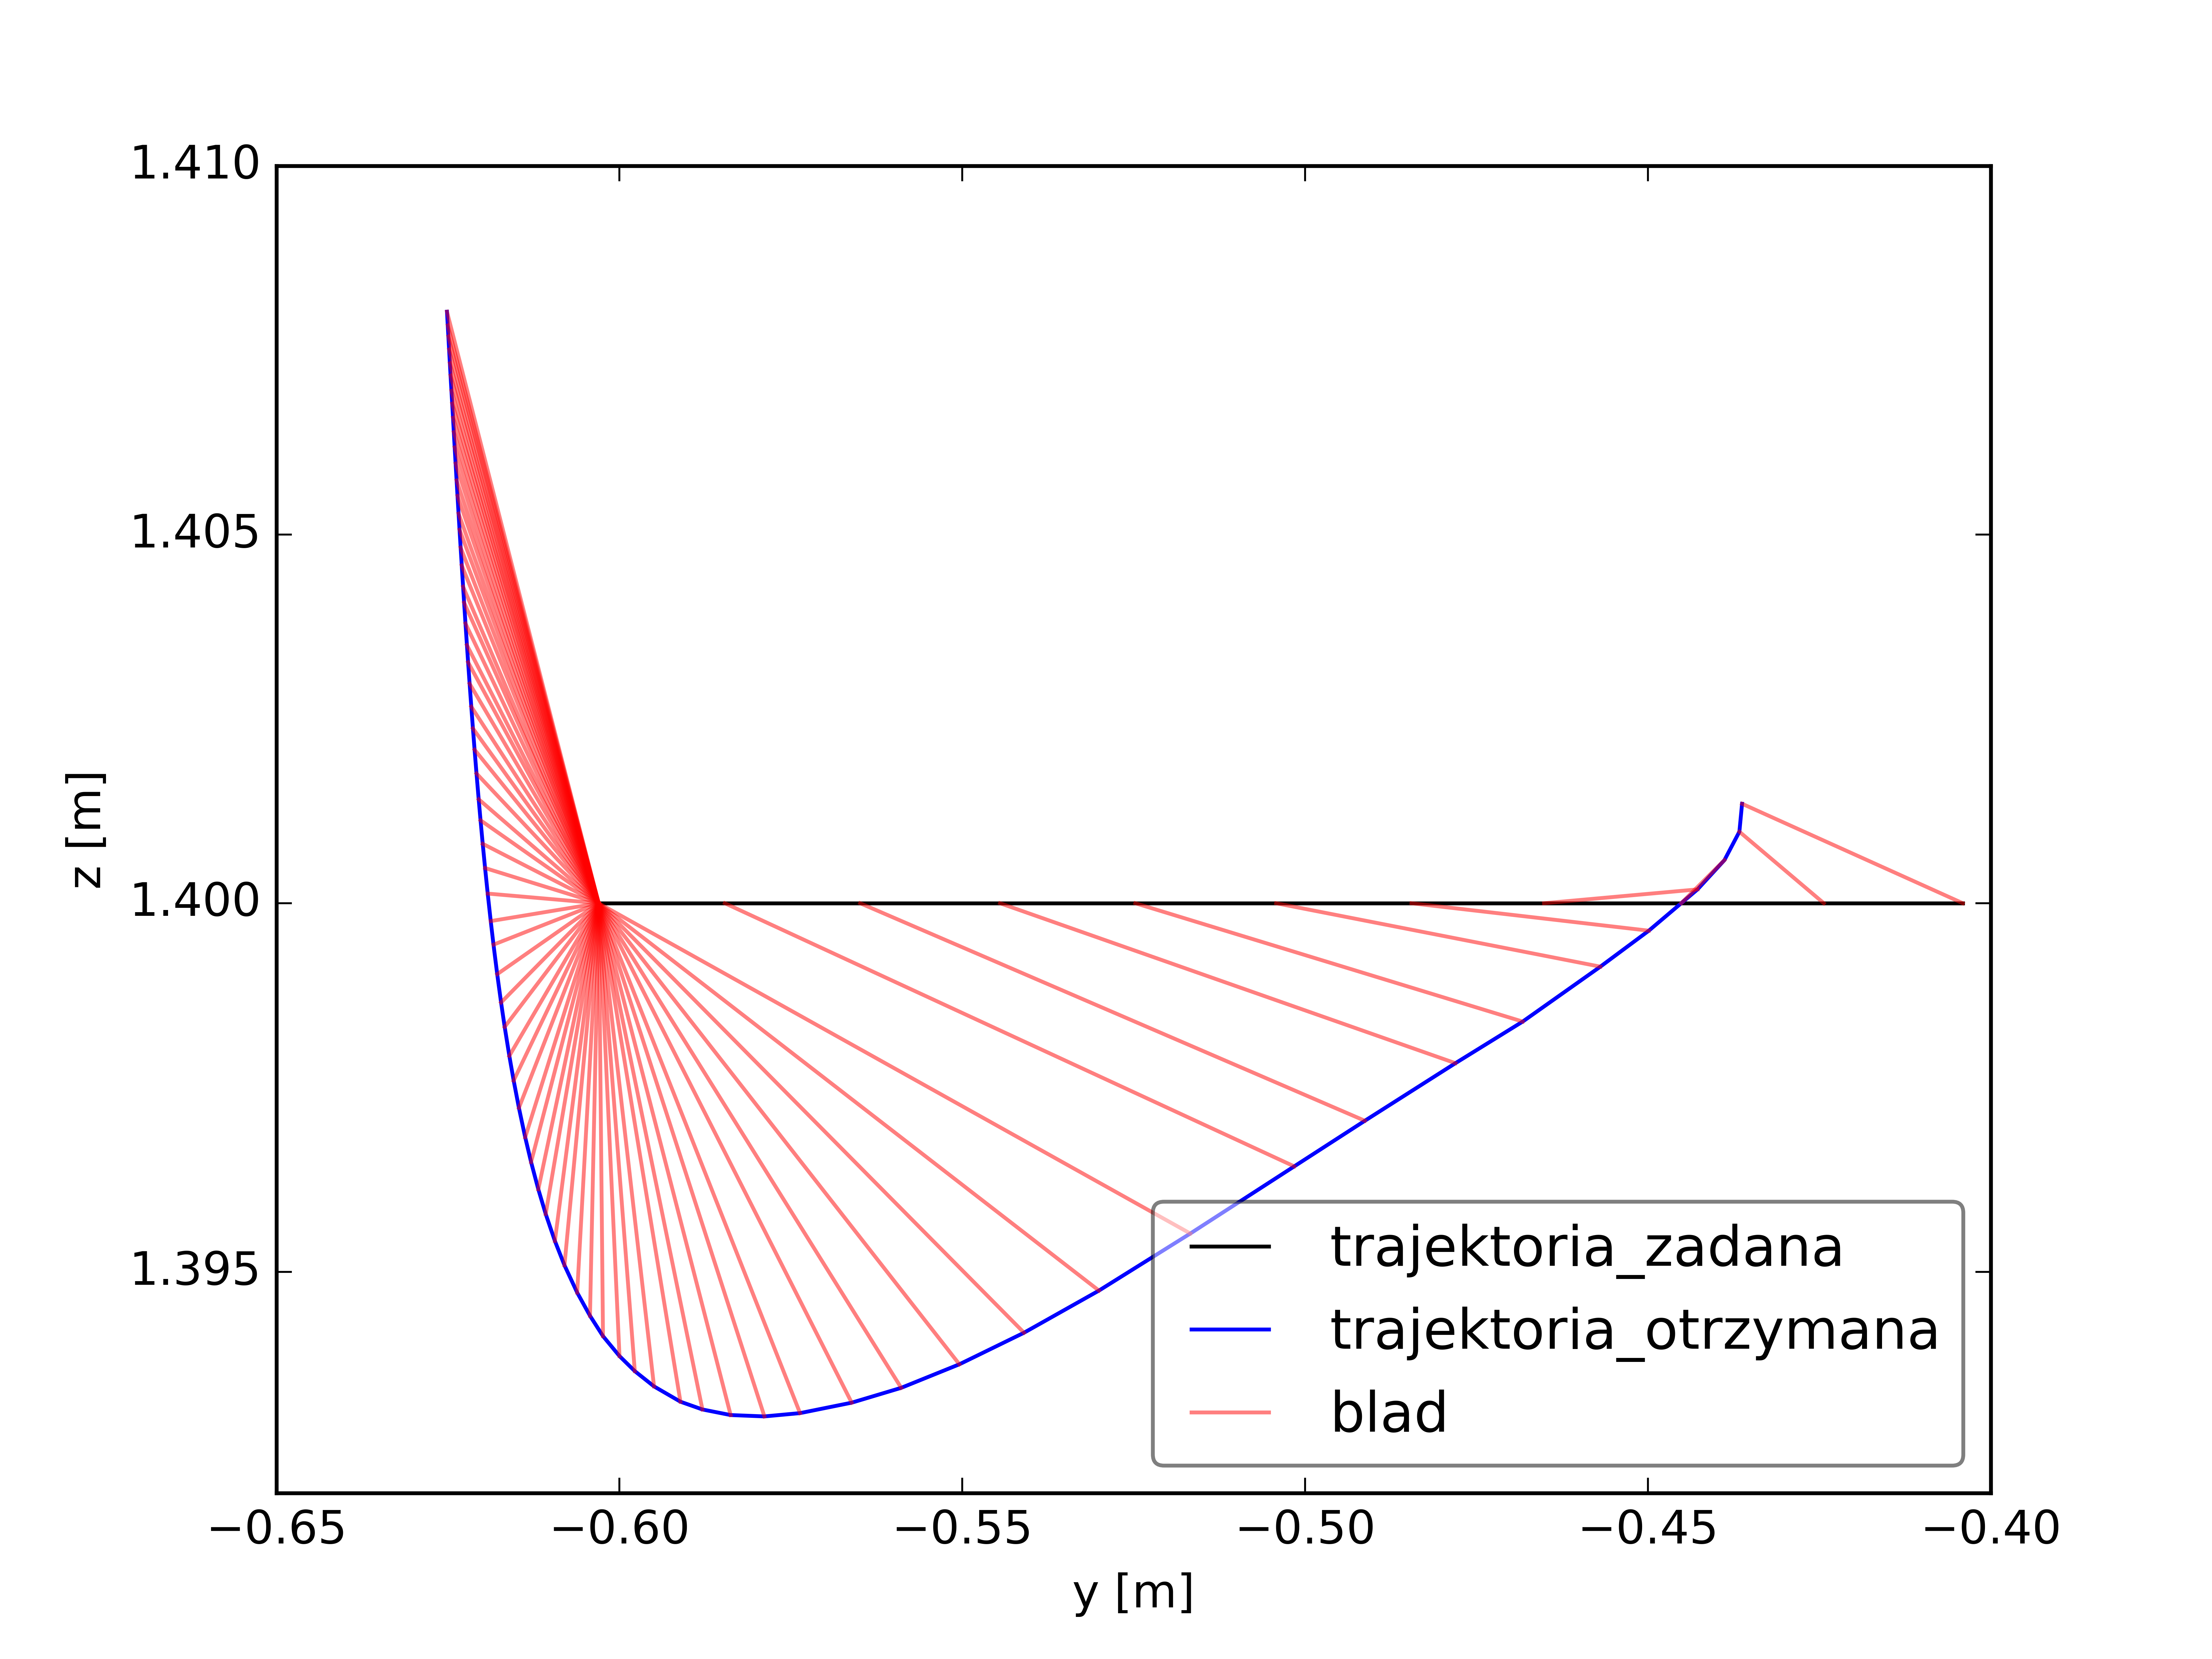
\includegraphics[width=.45\textwidth]{../../velma/przerobione_testy/out/w_bok_miekki/yz_ate_plot_podnoszenie_miekki_bez_brak.png}
	}
	\hfill
	\subfigure[Zalaczony algorytm kompnesacji]{
		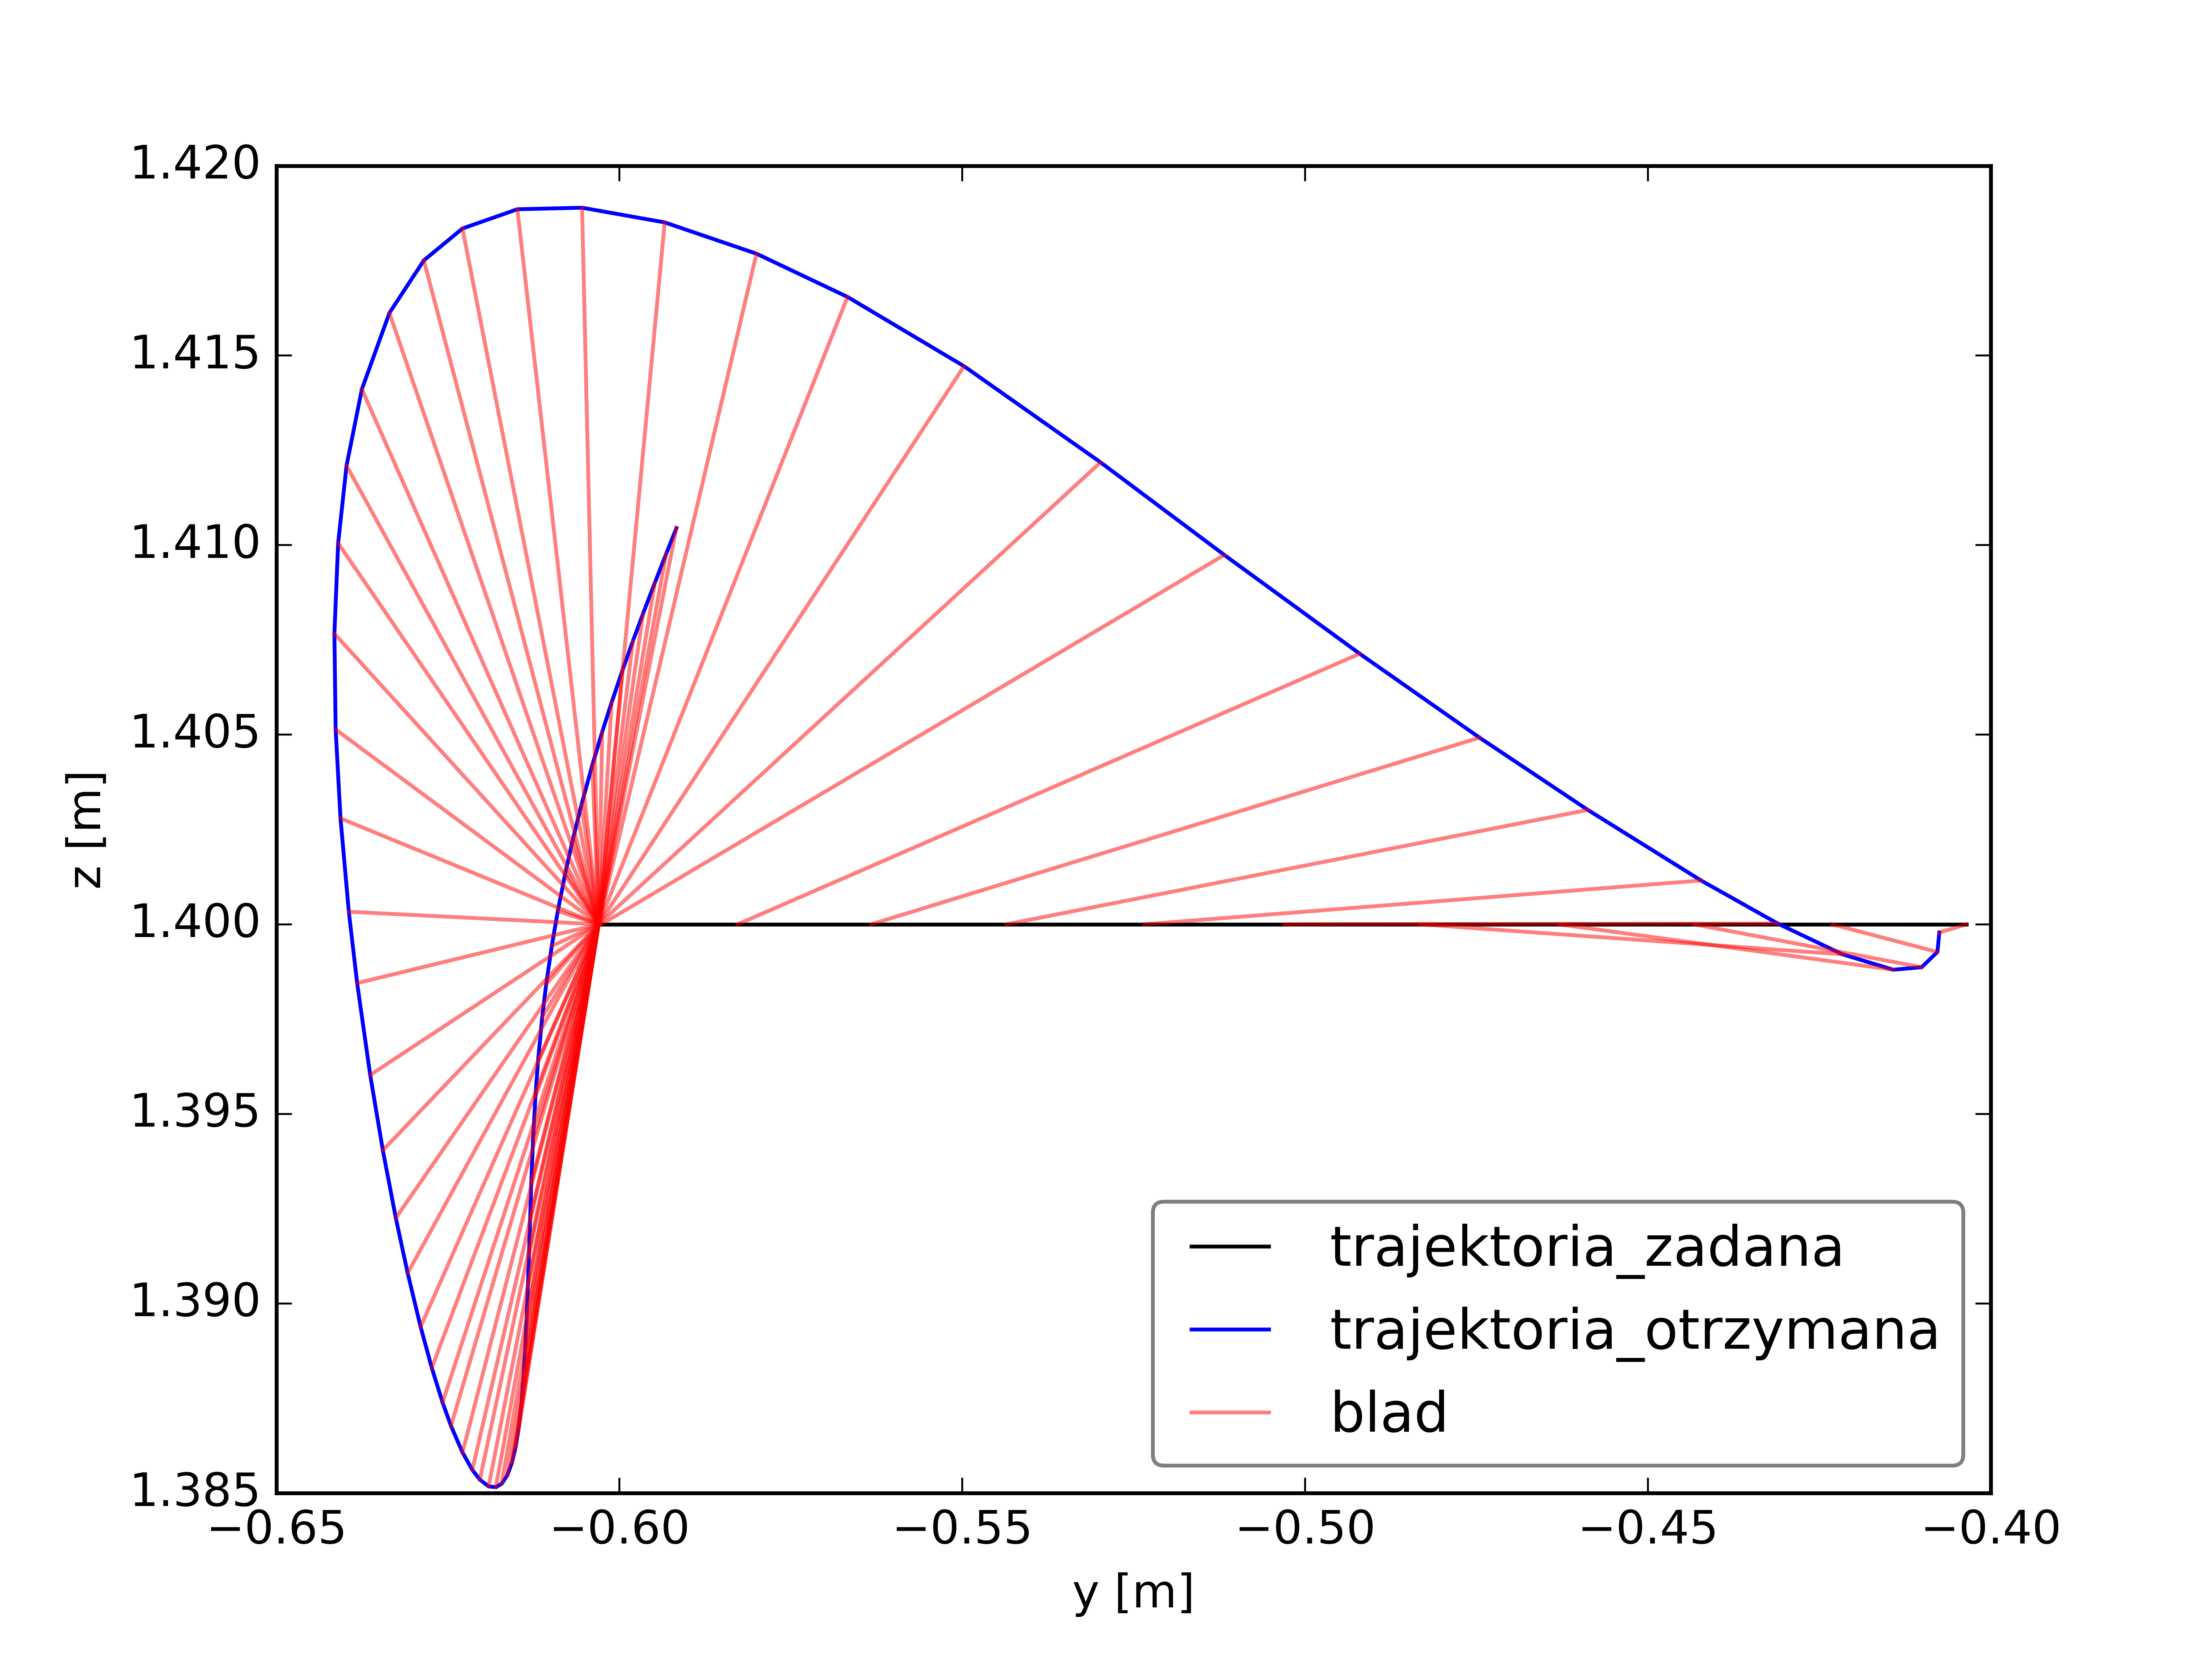
\includegraphics[width=.45\textwidth]{../../velma/przerobione_testy/out/w_bok_miekki/yz_ate_plot_podnoszenie_miekki_komp_brak.png}
	}
	\caption{Porownanie trajektorii chwytaka w osiach $Y$ i $Z$}
	\label{fig:w_bok_miekki_porow_komp}
\end{figure}

\begin{figure}[h]
	\centering
	\subfigure[Trajektoria z chwycona puszka]{
		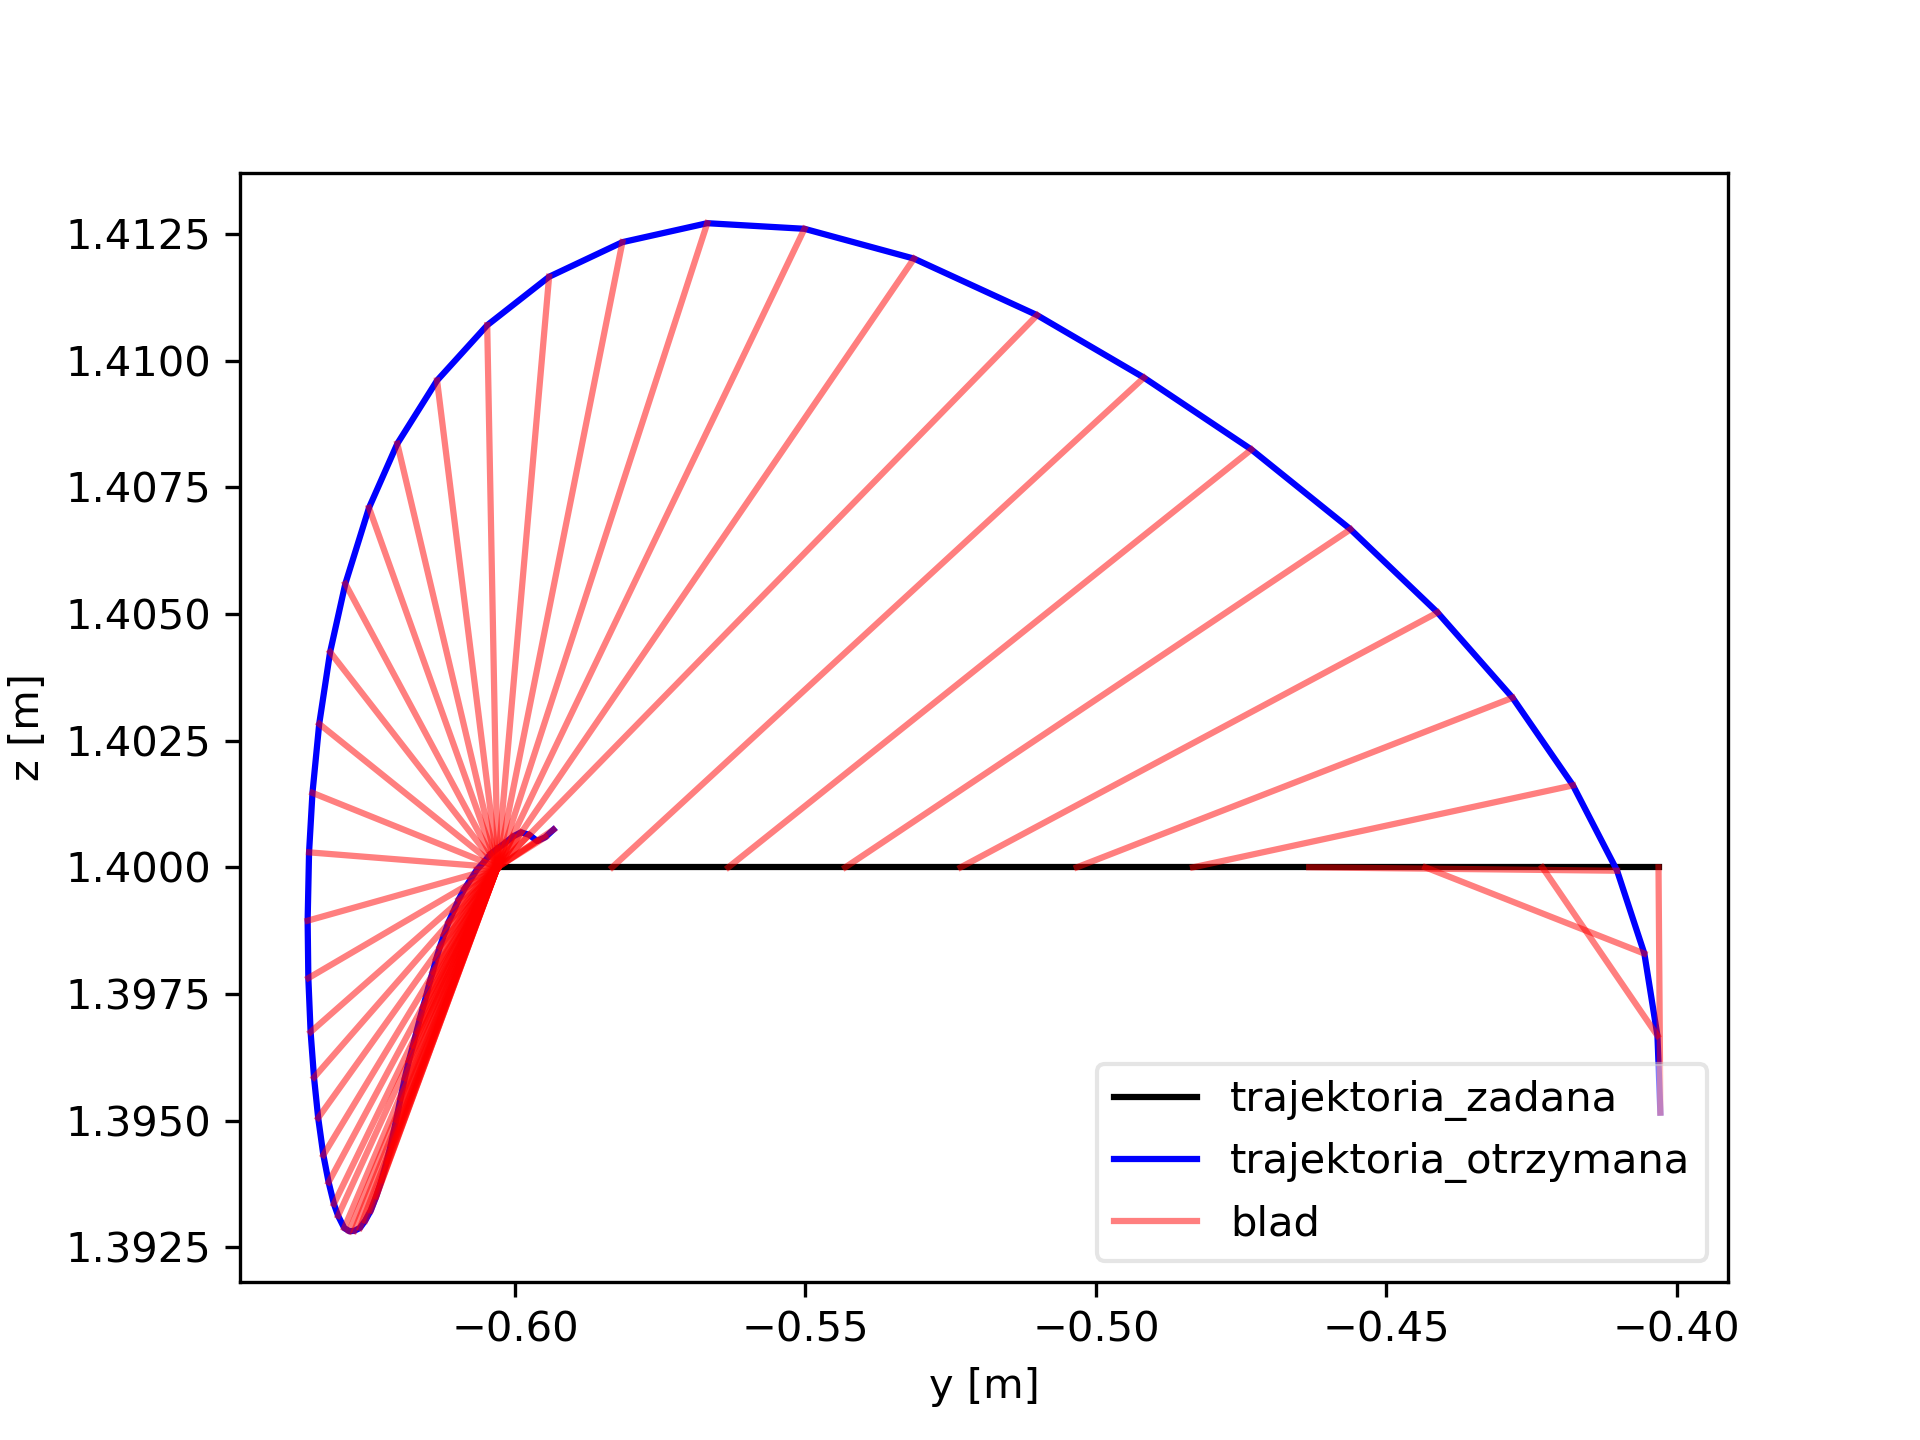
\includegraphics[width=.45\textwidth]{../../velma/przerobione_testy/out/w_bok_miekki/yz_ate_plot_podnoszenie_miekki_komp_piwo.png}
	}
	\hfill
	\subfigure[Trajektoria z chwycona wiertarka]{
		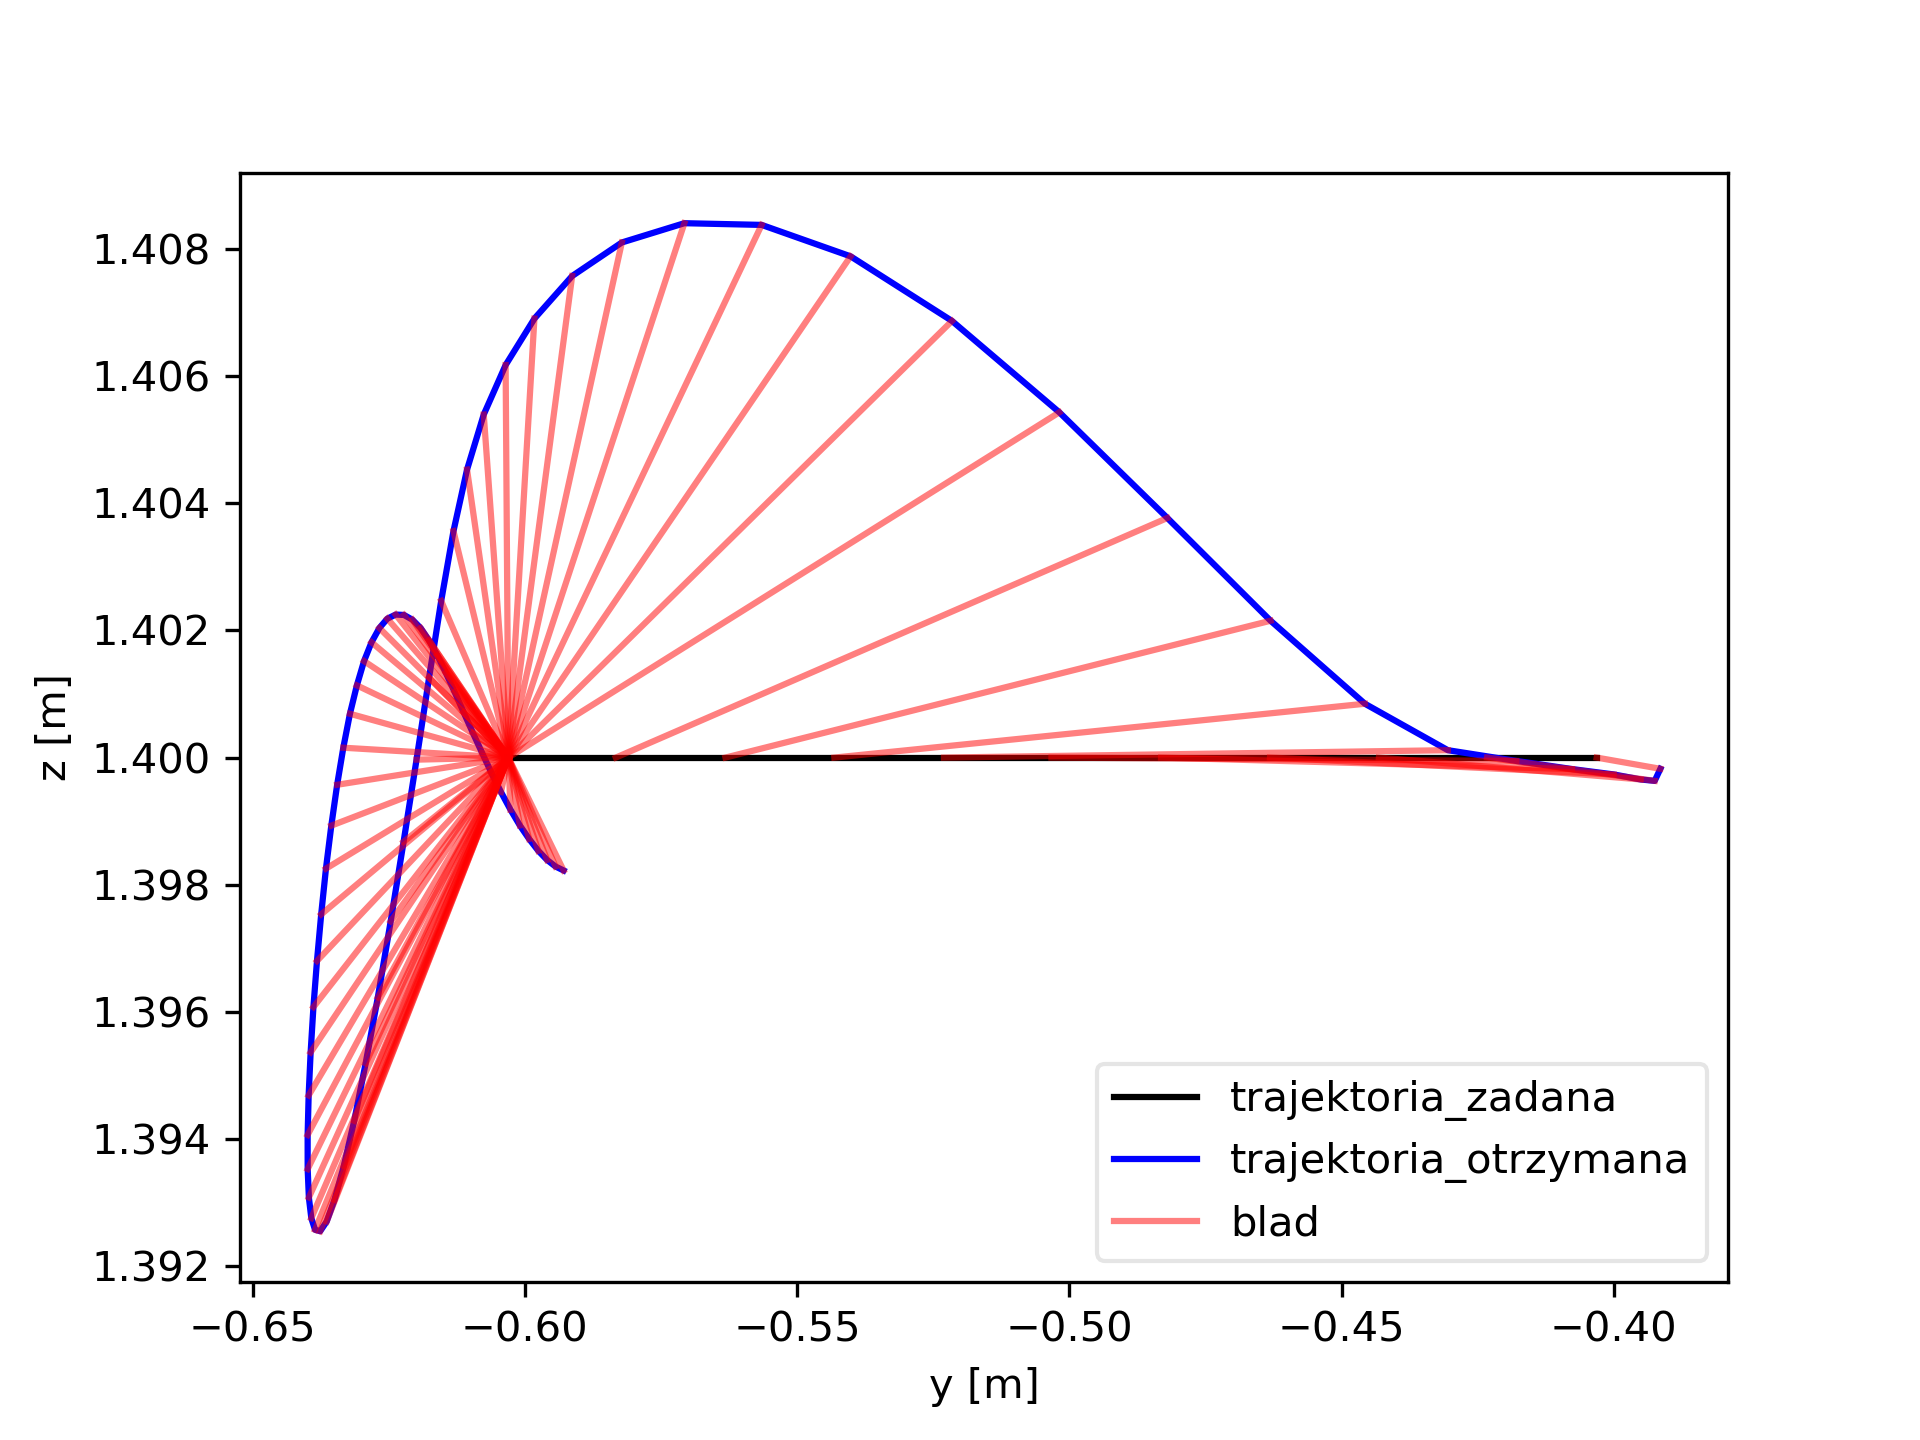
\includegraphics[width=.45\textwidth]{../../velma/przerobione_testy/out/w_bok_miekki/yz_ate_plot_podnoszenie_miekki_komp_wiertarka.png}
	}
	\caption{Porownanie trajektorii chwytaka w osiach $Y$ i $Z$}
	\label{fig:w_bok_miekki_porow_przedm}
\end{figure}


% \begin{figure}
% 	\centering
% 	\subfigure[Brak algorytmu kompensacji]{
% 		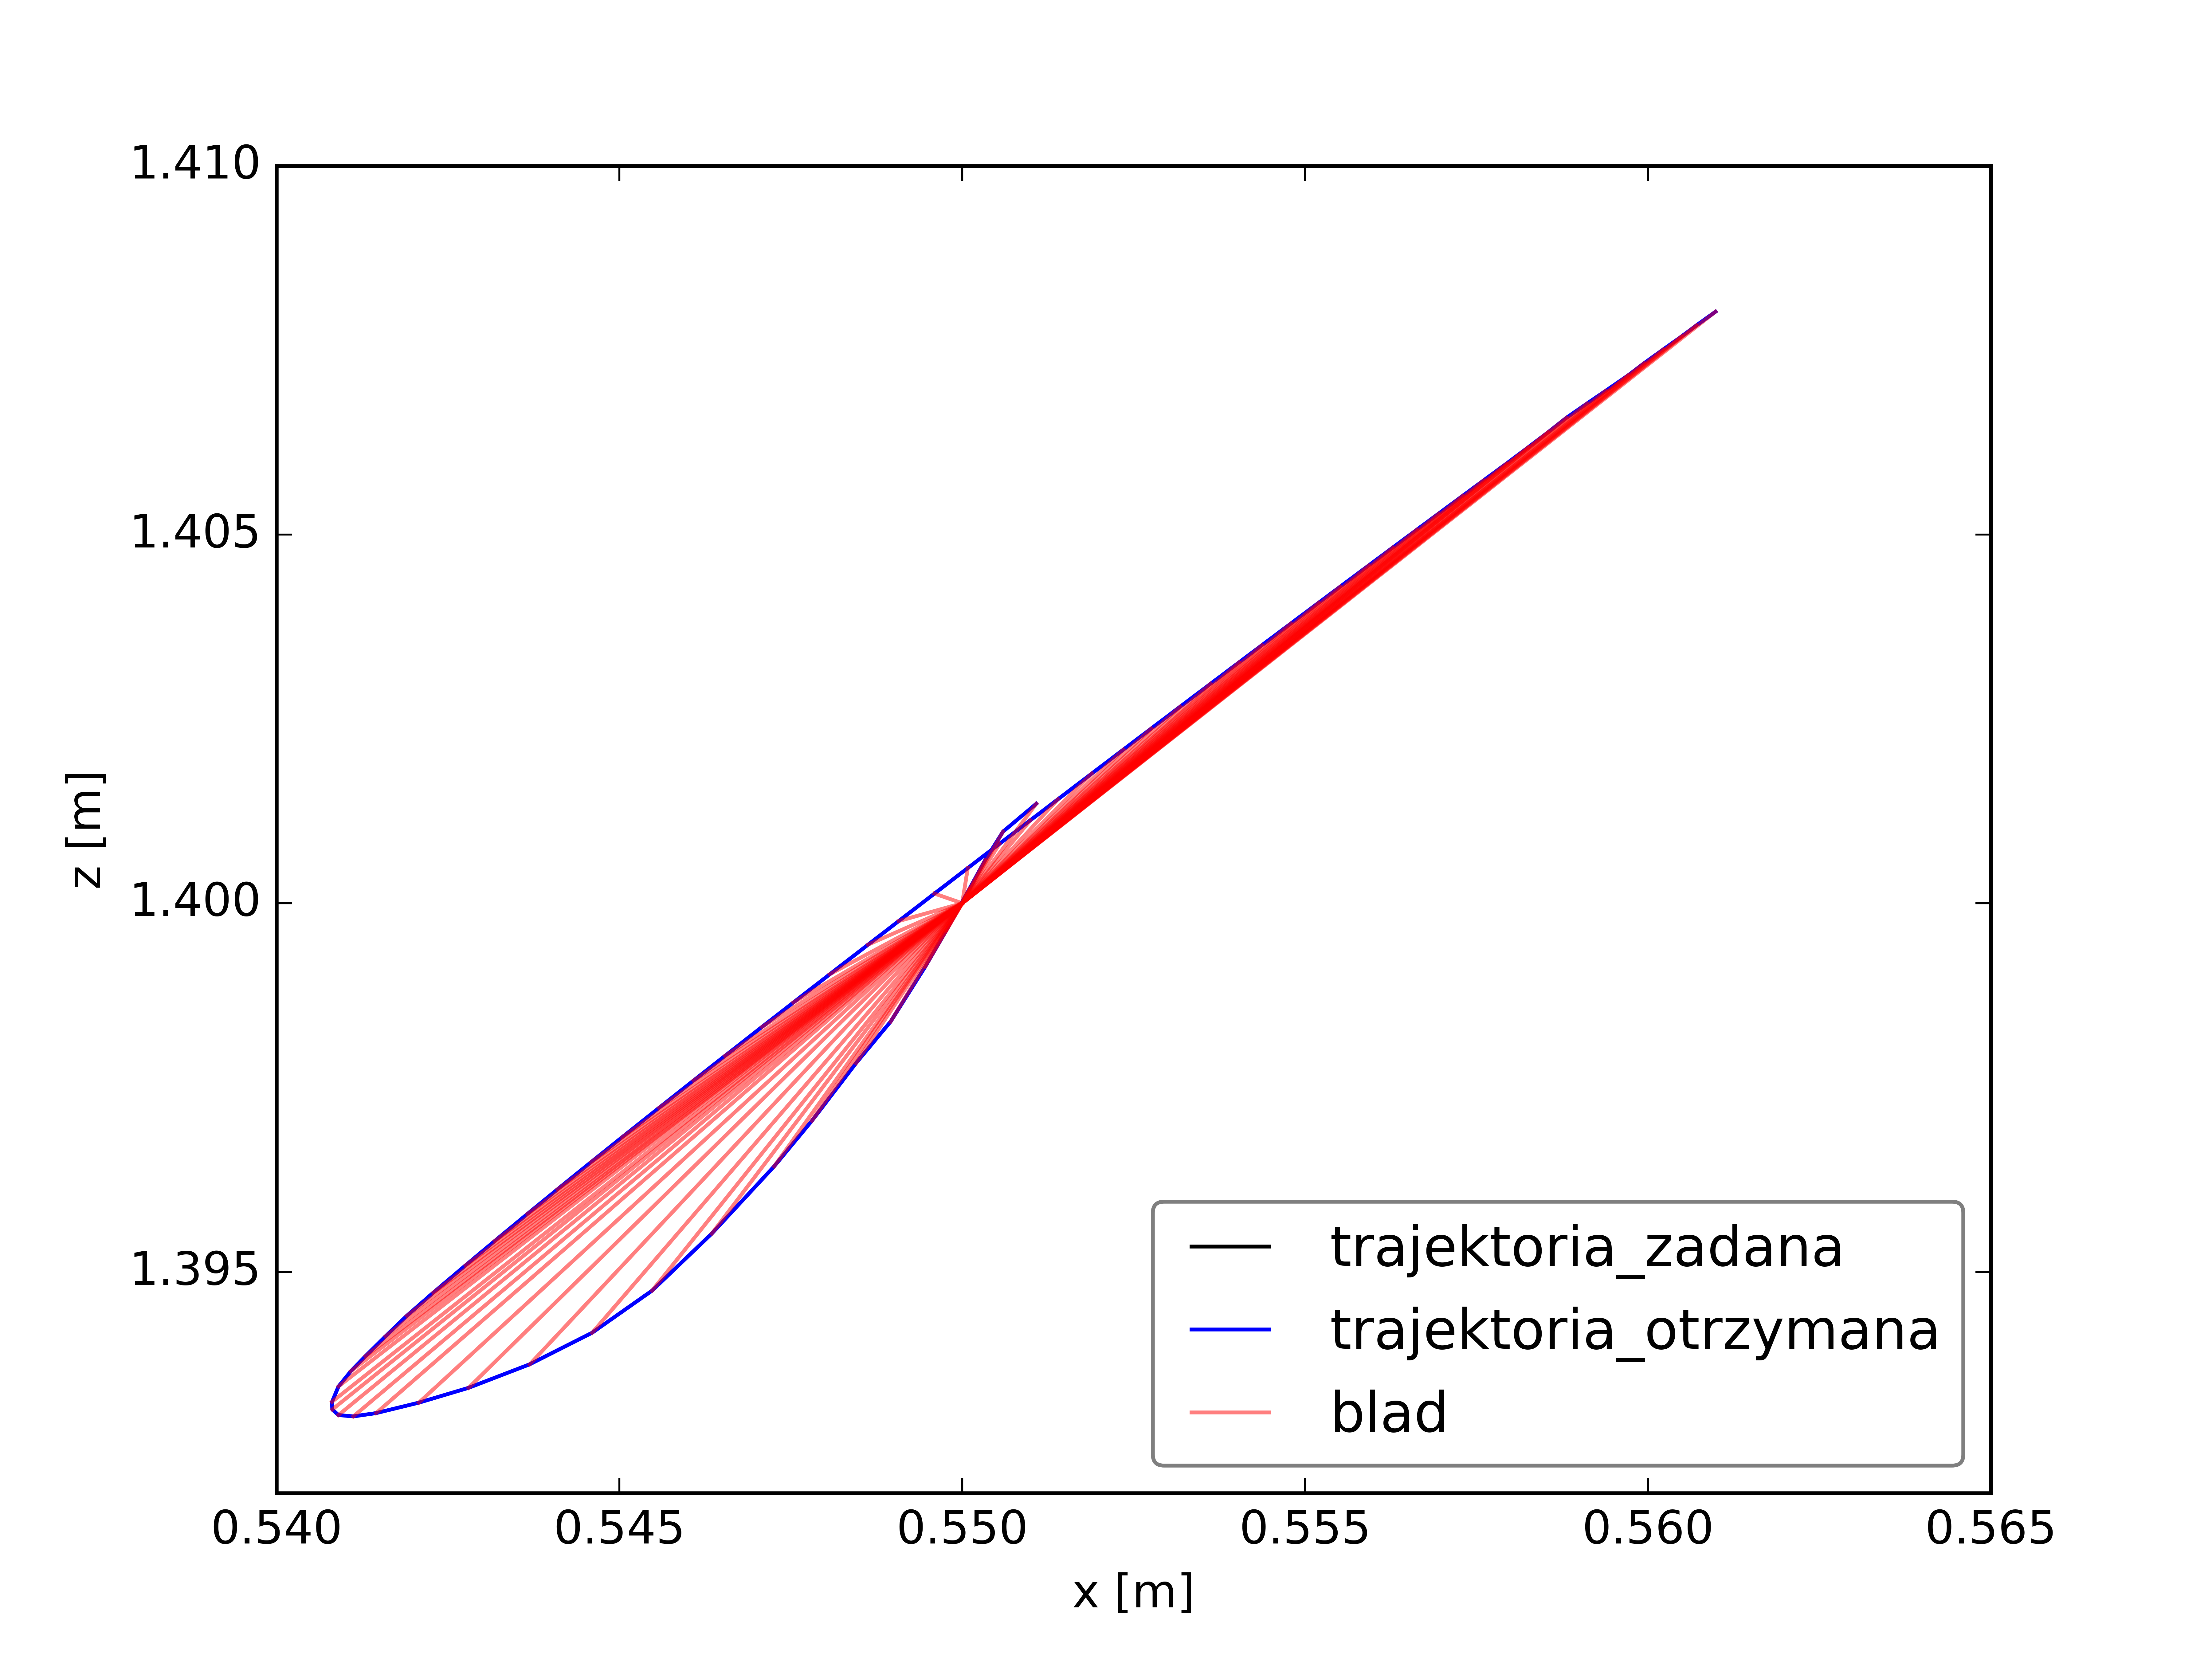
\includegraphics[width=.45\textwidth]{../../velma/przerobione_testy/out/w_bok_miekki/xz_ate_plot_podnoszenie_miekki_bez_brak.png}
% 	}
% 	\hfill
% 	\subfigure[Zalaczony algorytm kompnesacji]{
% 		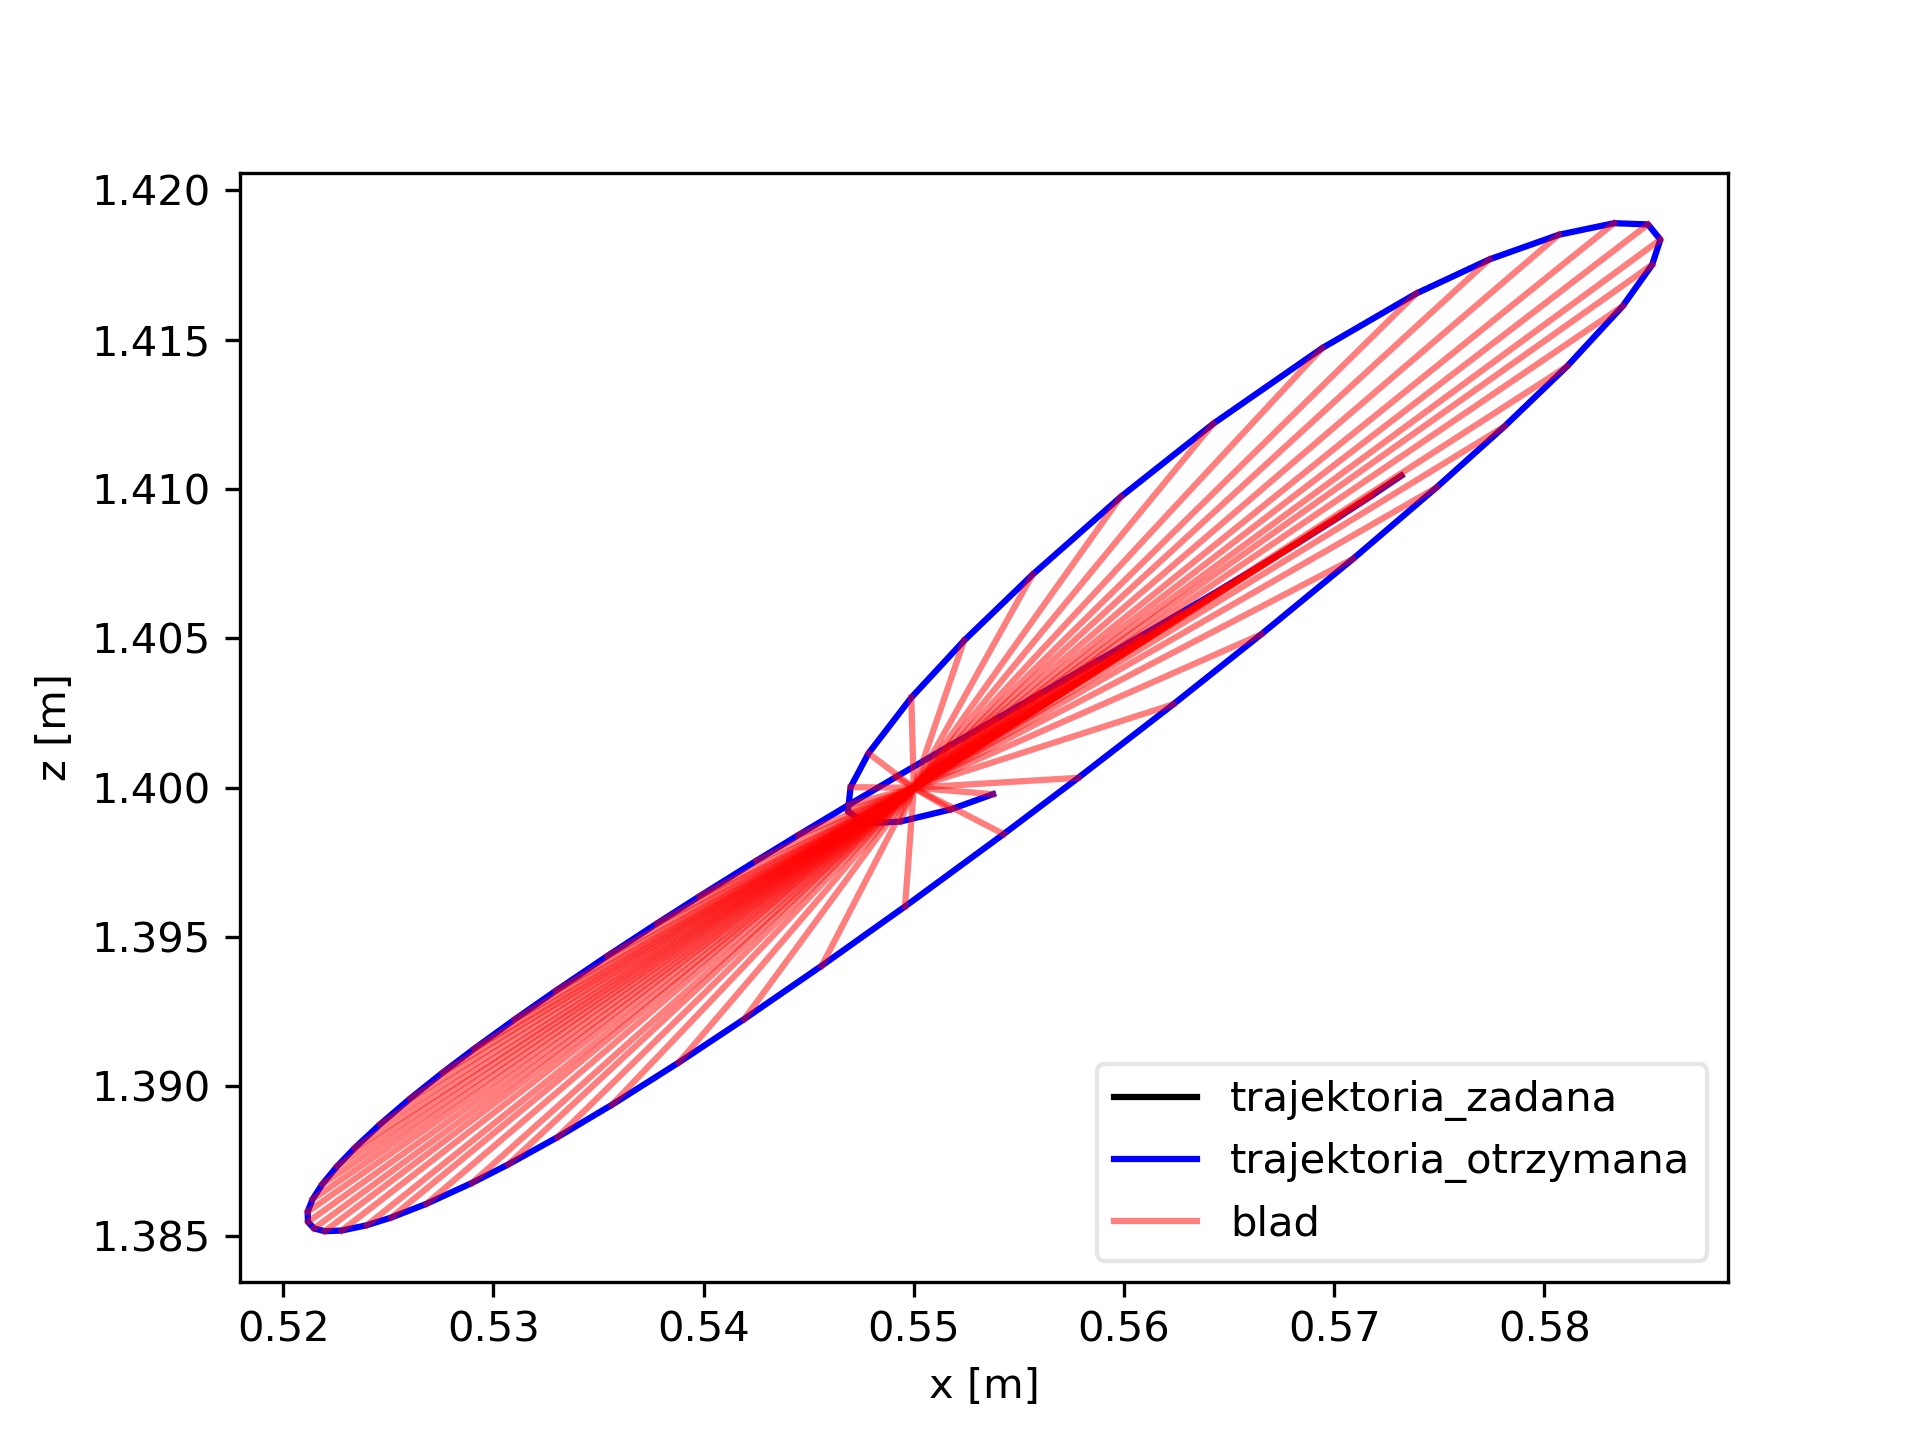
\includegraphics[width=.45\textwidth]{../../velma/przerobione_testy/out/w_bok_miekki/xz_ate_plot_podnoszenie_miekki_komp_brak.png}
% 	}
% 	\caption{Porownanie trajektorii chwytaka w osiach $X$ i $Z$}
% 	\label{fig:w_bok_miekki_porow_komp_bok}
% \end{figure}

% \begin{figure}
% 	\centering
% 	\subfigure[Trajektoria z chwycona puszka]{
% 		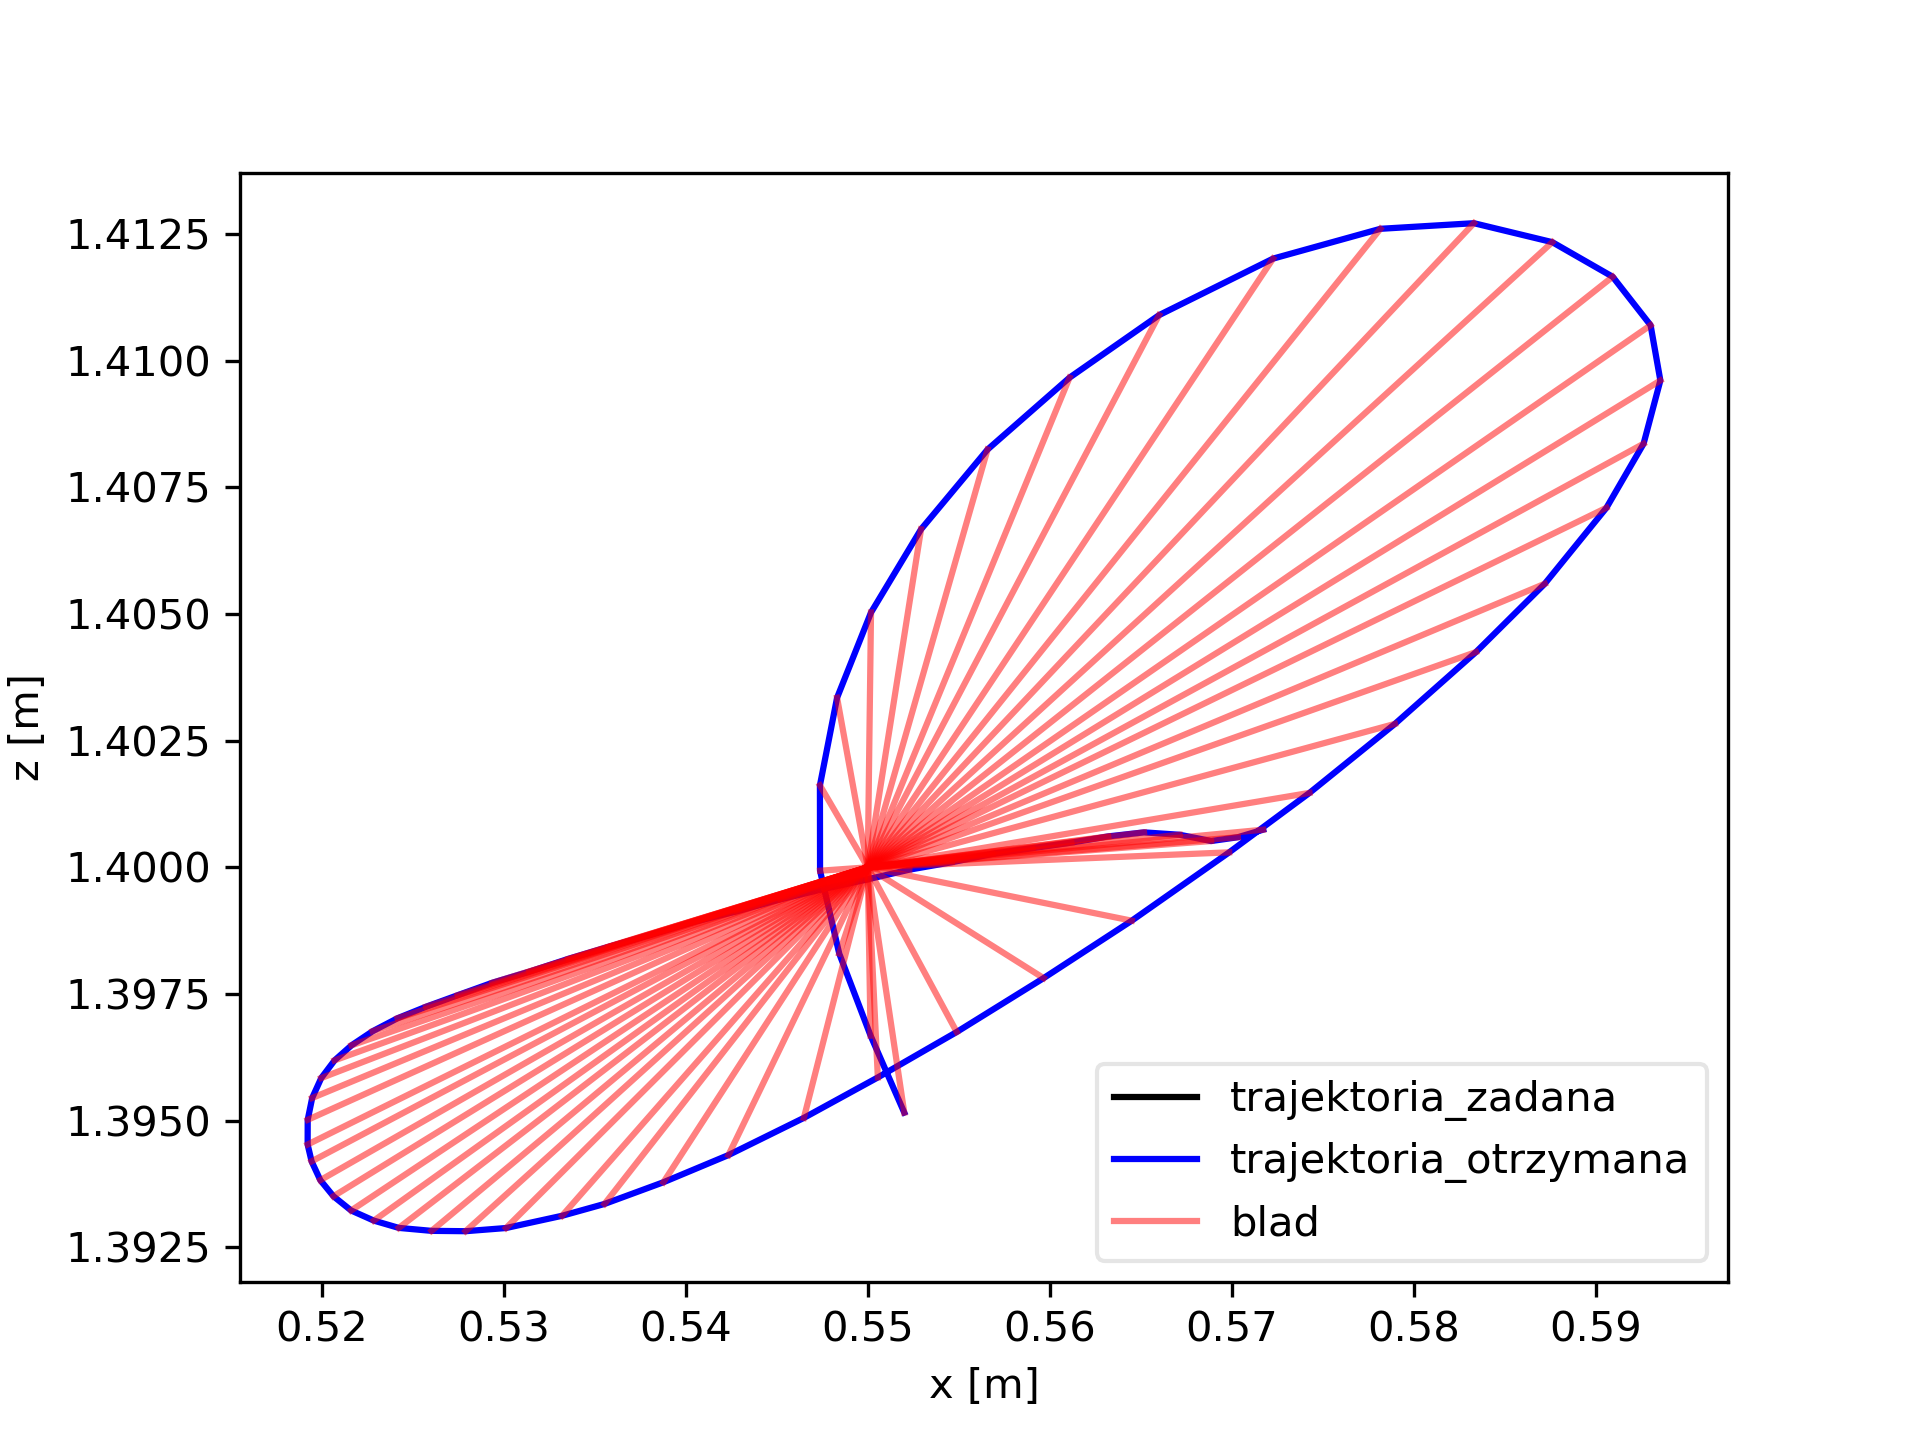
\includegraphics[width=.45\textwidth]{../../velma/przerobione_testy/out/w_bok_miekki/xz_ate_plot_podnoszenie_miekki_komp_piwo.png}
% 	}
% 	\hfill
% 	\subfigure[Trajektoria z chwycona wiertarka]{
% 		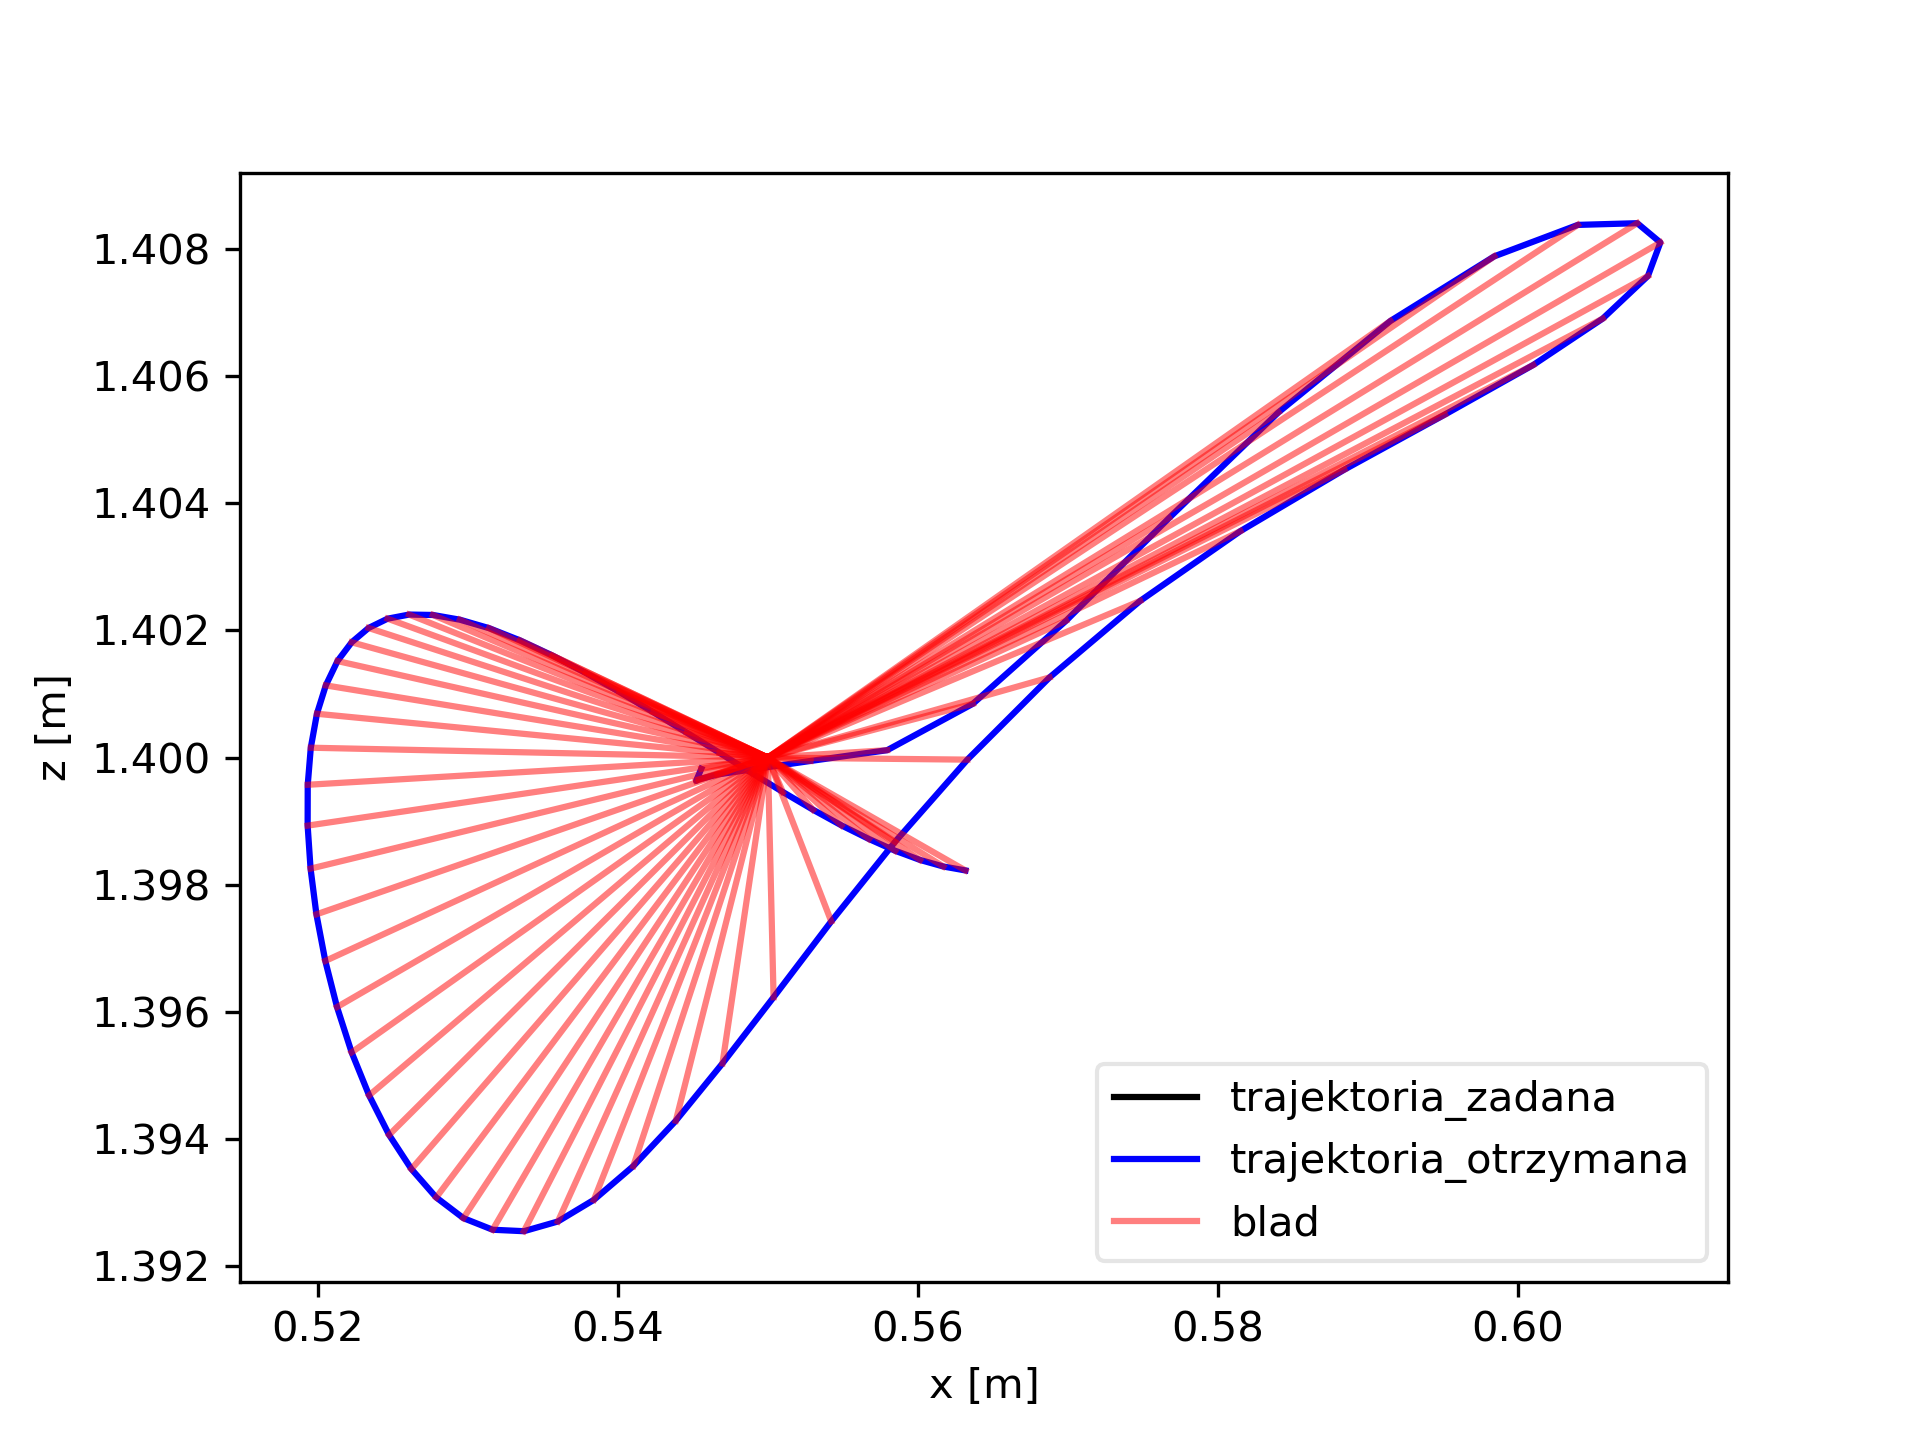
\includegraphics[width=.45\textwidth]{../../velma/przerobione_testy/out/w_bok_miekki/xz_ate_plot_podnoszenie_miekki_komp_wiertarka.png}
% 	}
% 	\caption{Porownanie trajektorii chwytaka w osiach $X$ i $Z$}
% 	\label{fig:w_bok_miekki_porow_przedm_bok}
% \end{figure}

\begin{figure}[h]
	\centering
	\subfigure[Rzut na wprost]{
		\label{fig:w_bok_miekki_porow_zbiorcze_a}
		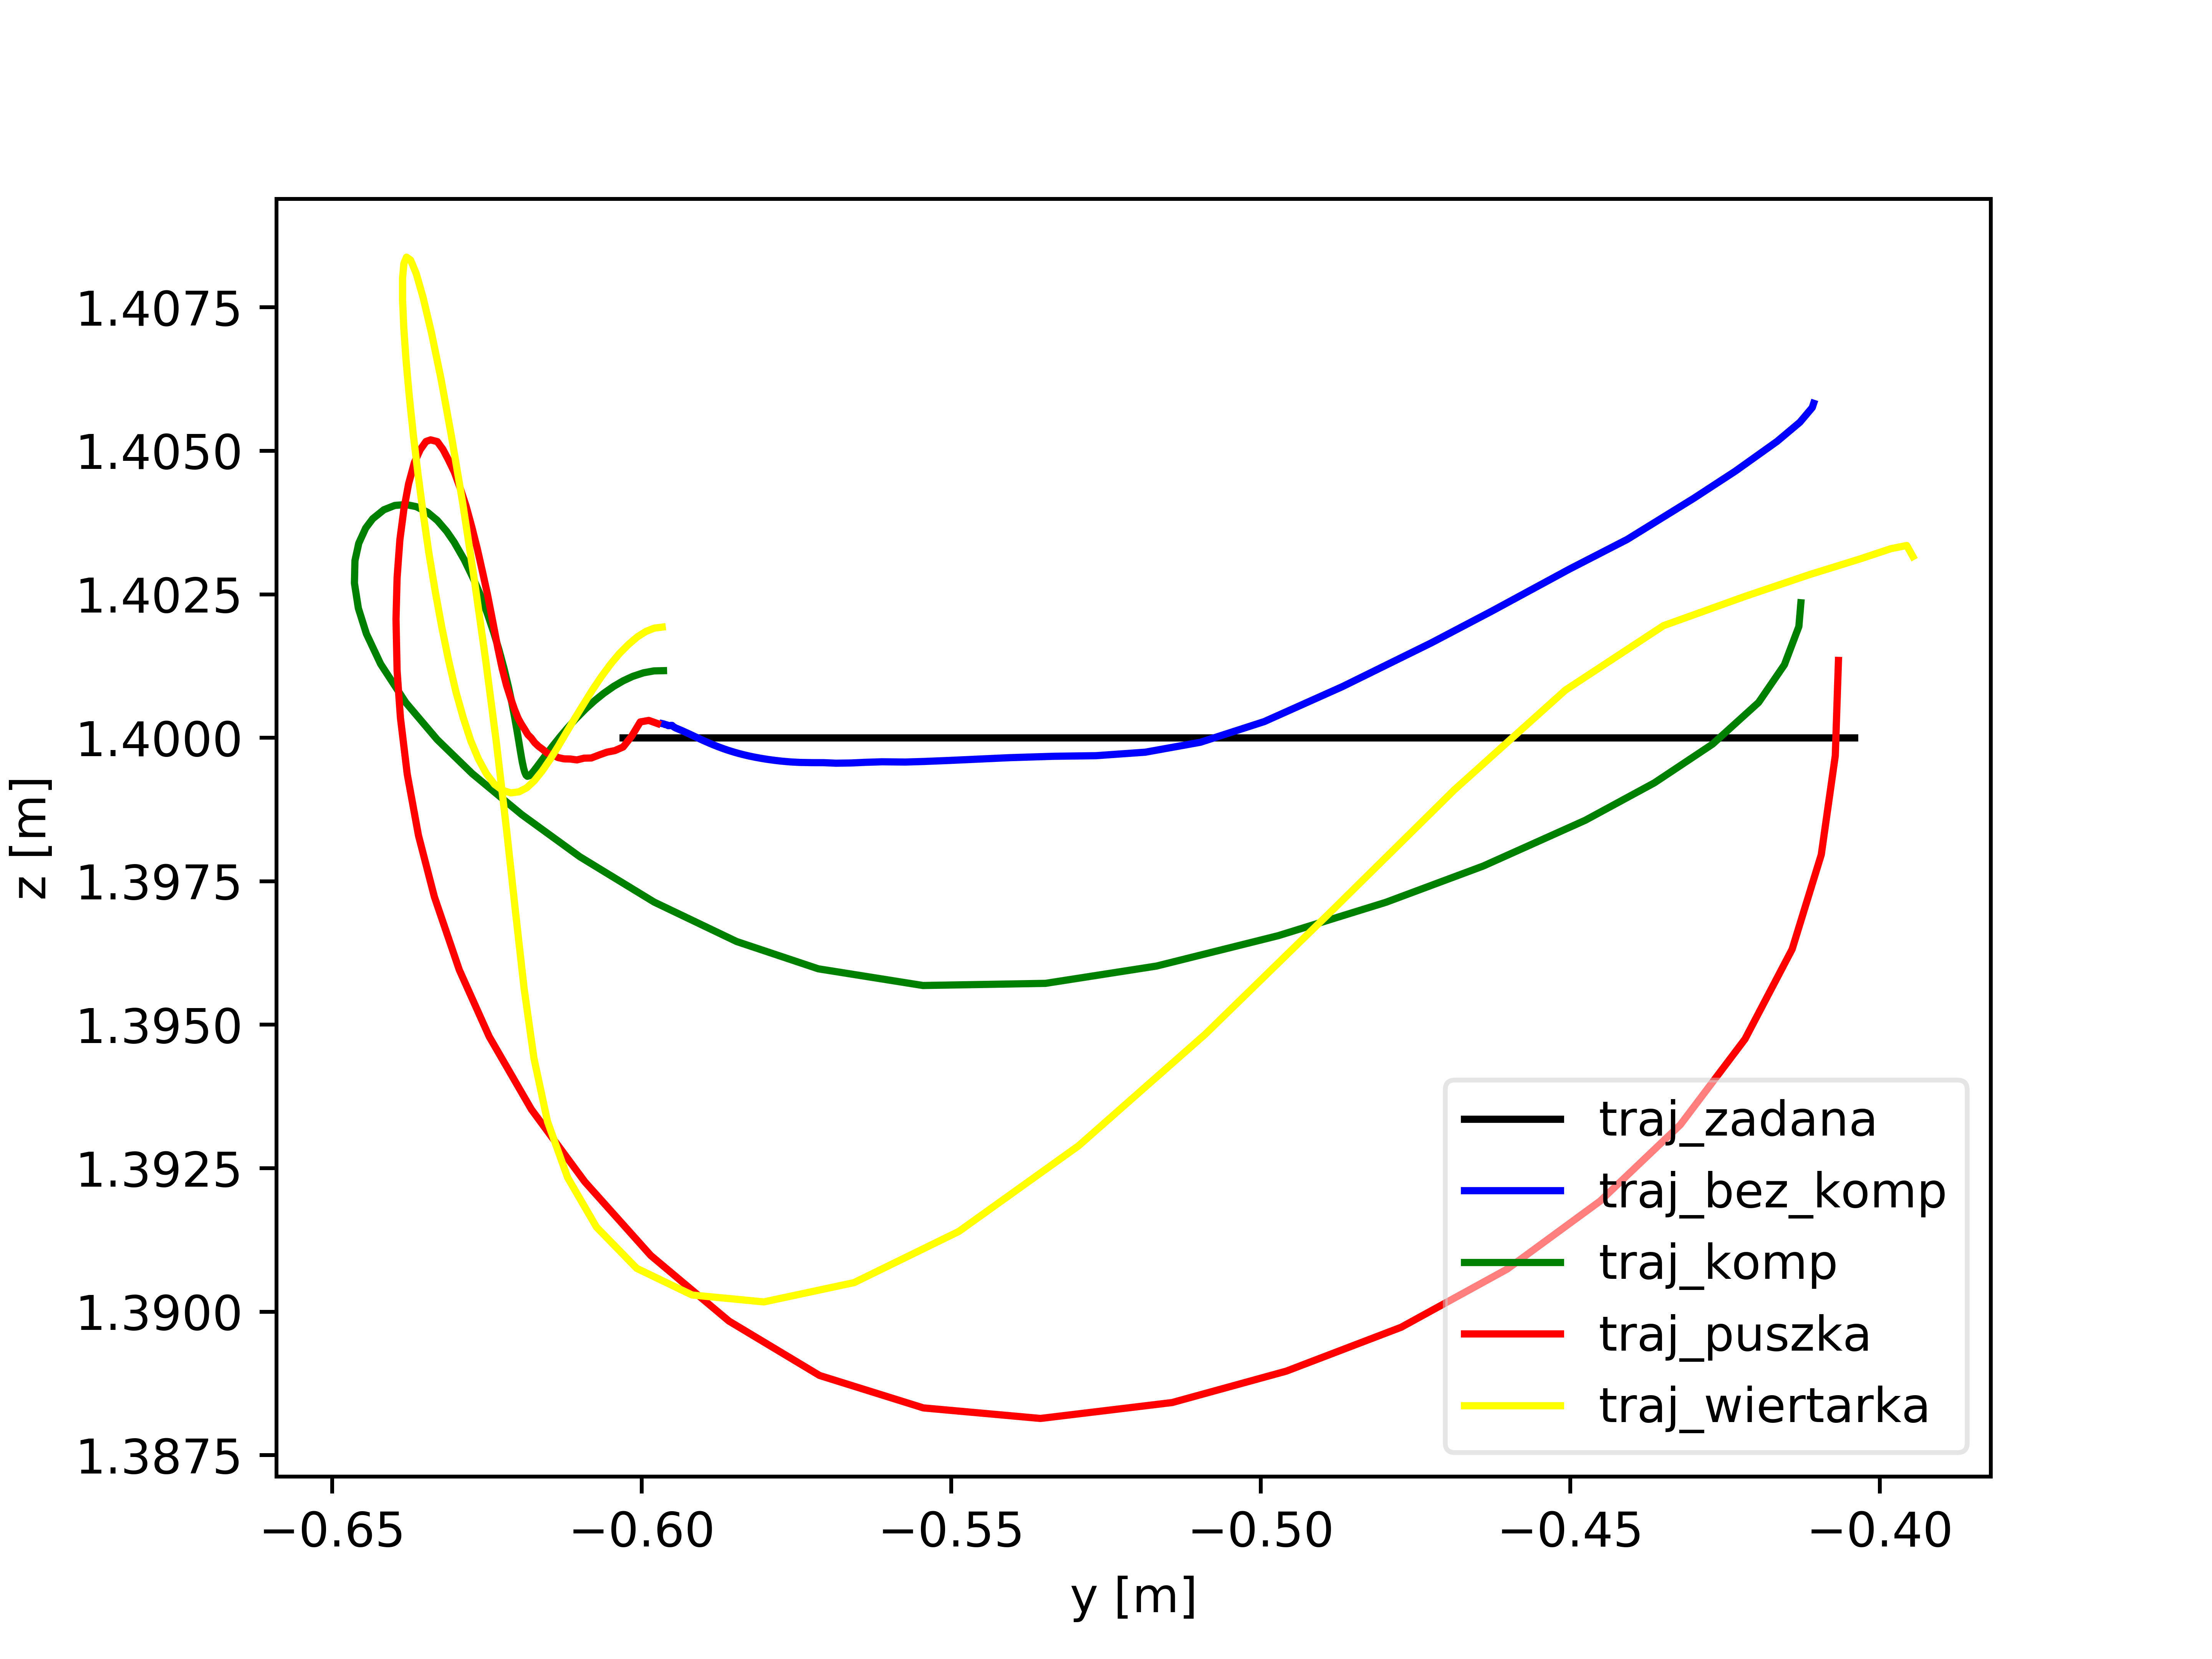
\includegraphics[width=.45\textwidth]{../../velma/przerobione_testy/out/w_bok_miekki/common_yz.png}
	}
	\hfill
	% \subfigure[Rzut z boku]{
	% 	\label{fig:w_bok_miekki_porow_zbiorcze_b}
	% 	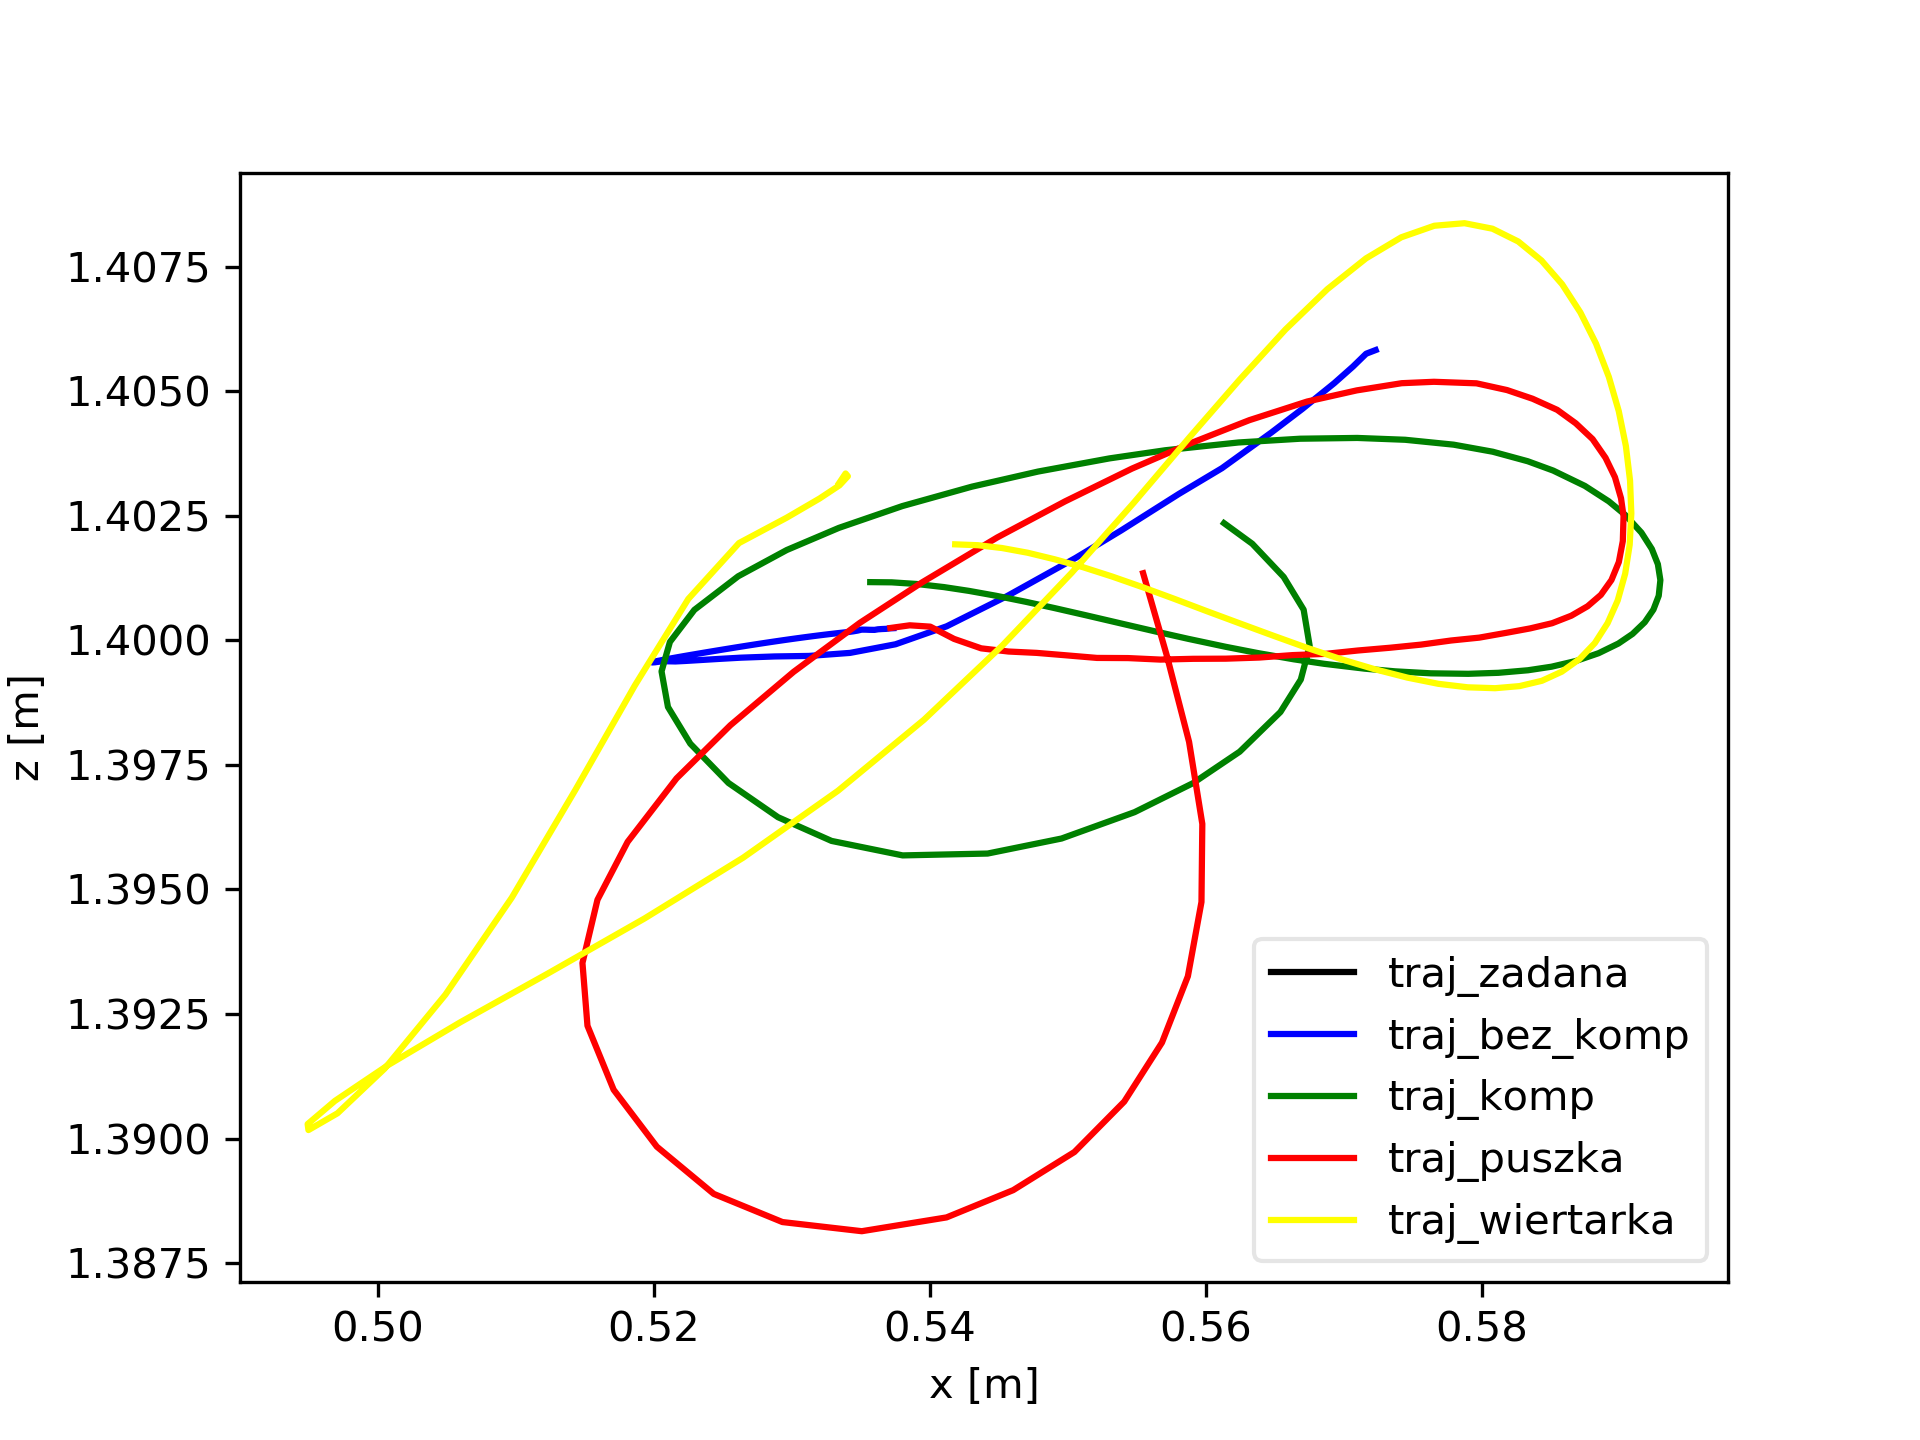
\includegraphics[width=.45\textwidth]{../../velma/przerobione_testy/out/w_bok_miekki/common_xz.png}
	% }
	\caption{Porowanie wszystkich trajektorii.}
	\label{fig:w_bok_miekki_porow_zbiorcze}
\end{figure}


\subsection{Ruch do gory}

Eksperyment ma przetestowac zachowanie algorytmu kompensacji przy ruchu koncowki do gory (rys. \ref{fig:do_gory_a}, \ref{fig:do_gory_rot}). Jest to dla algorytmu potencjalnie trudny ruch z przez sile grawitacji dzialajaca wlasnie w tej osi. Trajektoria ruchu w rzucie APE zostala zaprezentowana na rys. \ref{fig:do_gory_porow_komp}, \ref{fig:do_gory_porow_przedm} i \ref{fig:do_gory_porow_zbiorcze_a}.

\begin{figure}[h]
	\centering
	\subfigure[Os $X$]{
		\label{fig:do_gory_ax}
		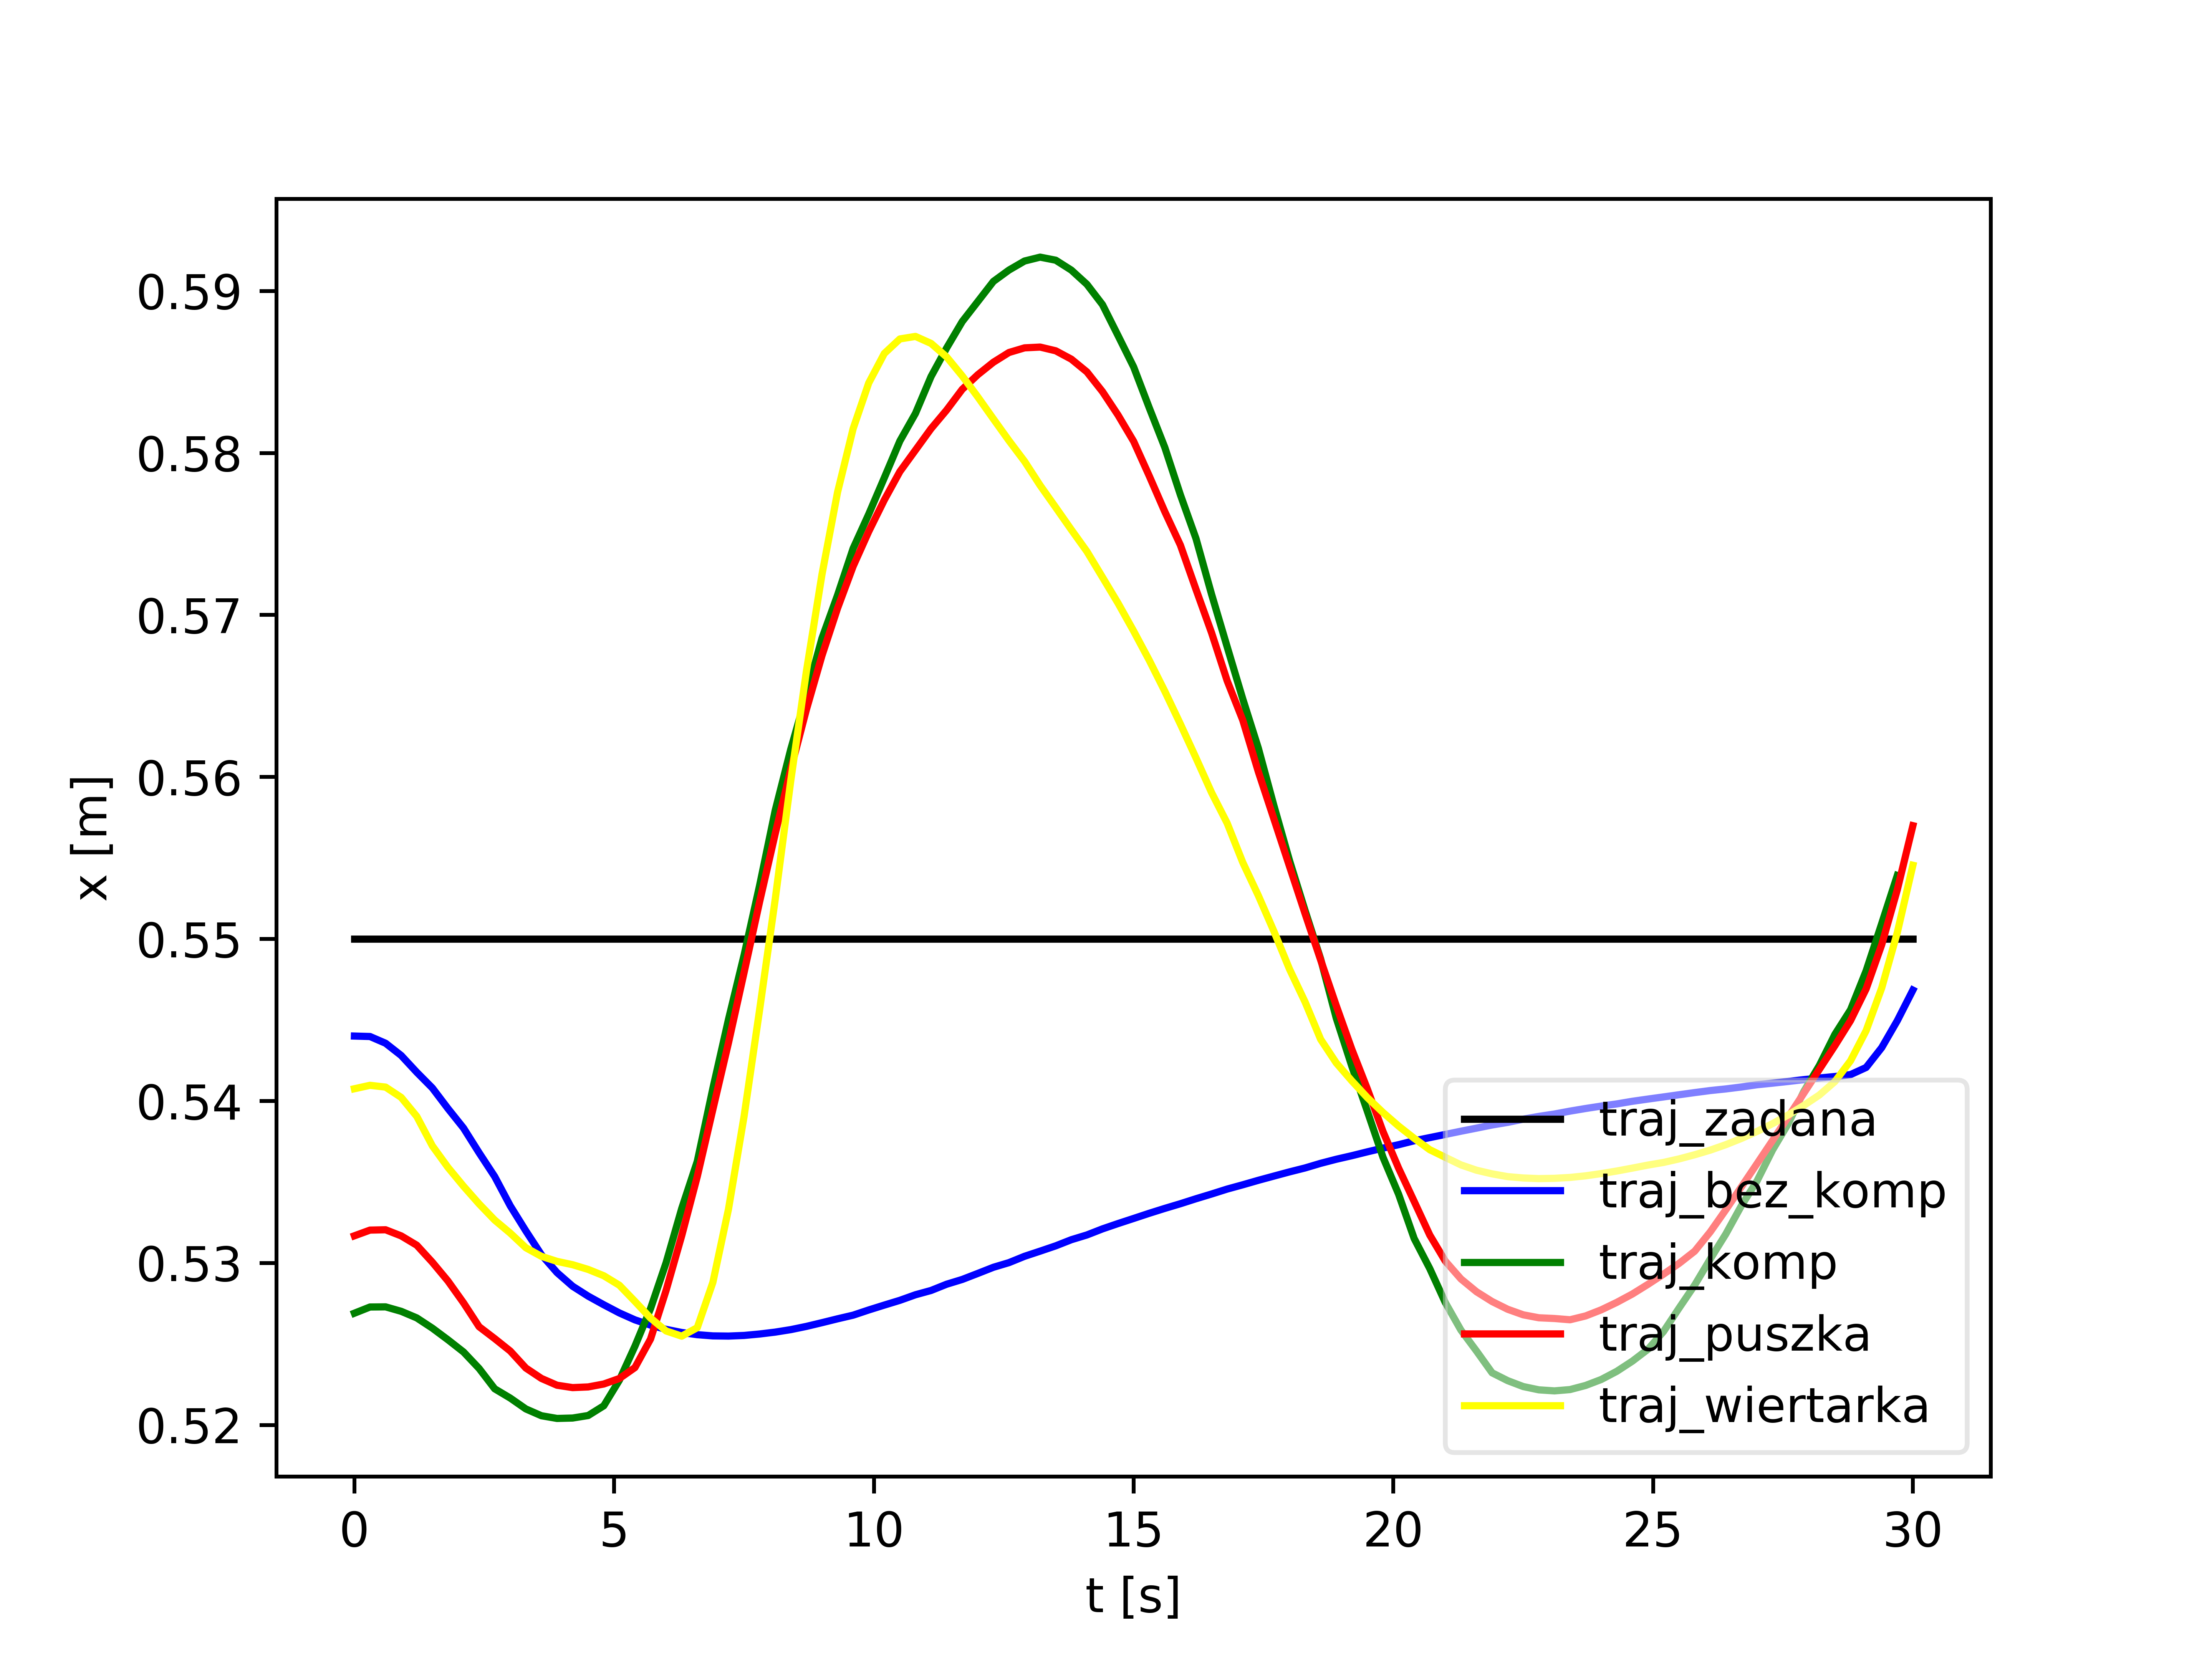
\includegraphics[width=.45\textwidth]{../../velma/przerobione_testy/out/do_gory/common_ax.png}
	}
	\hfill
	\subfigure[Os $Y$]{
		\label{fig:do_gory_ay}
		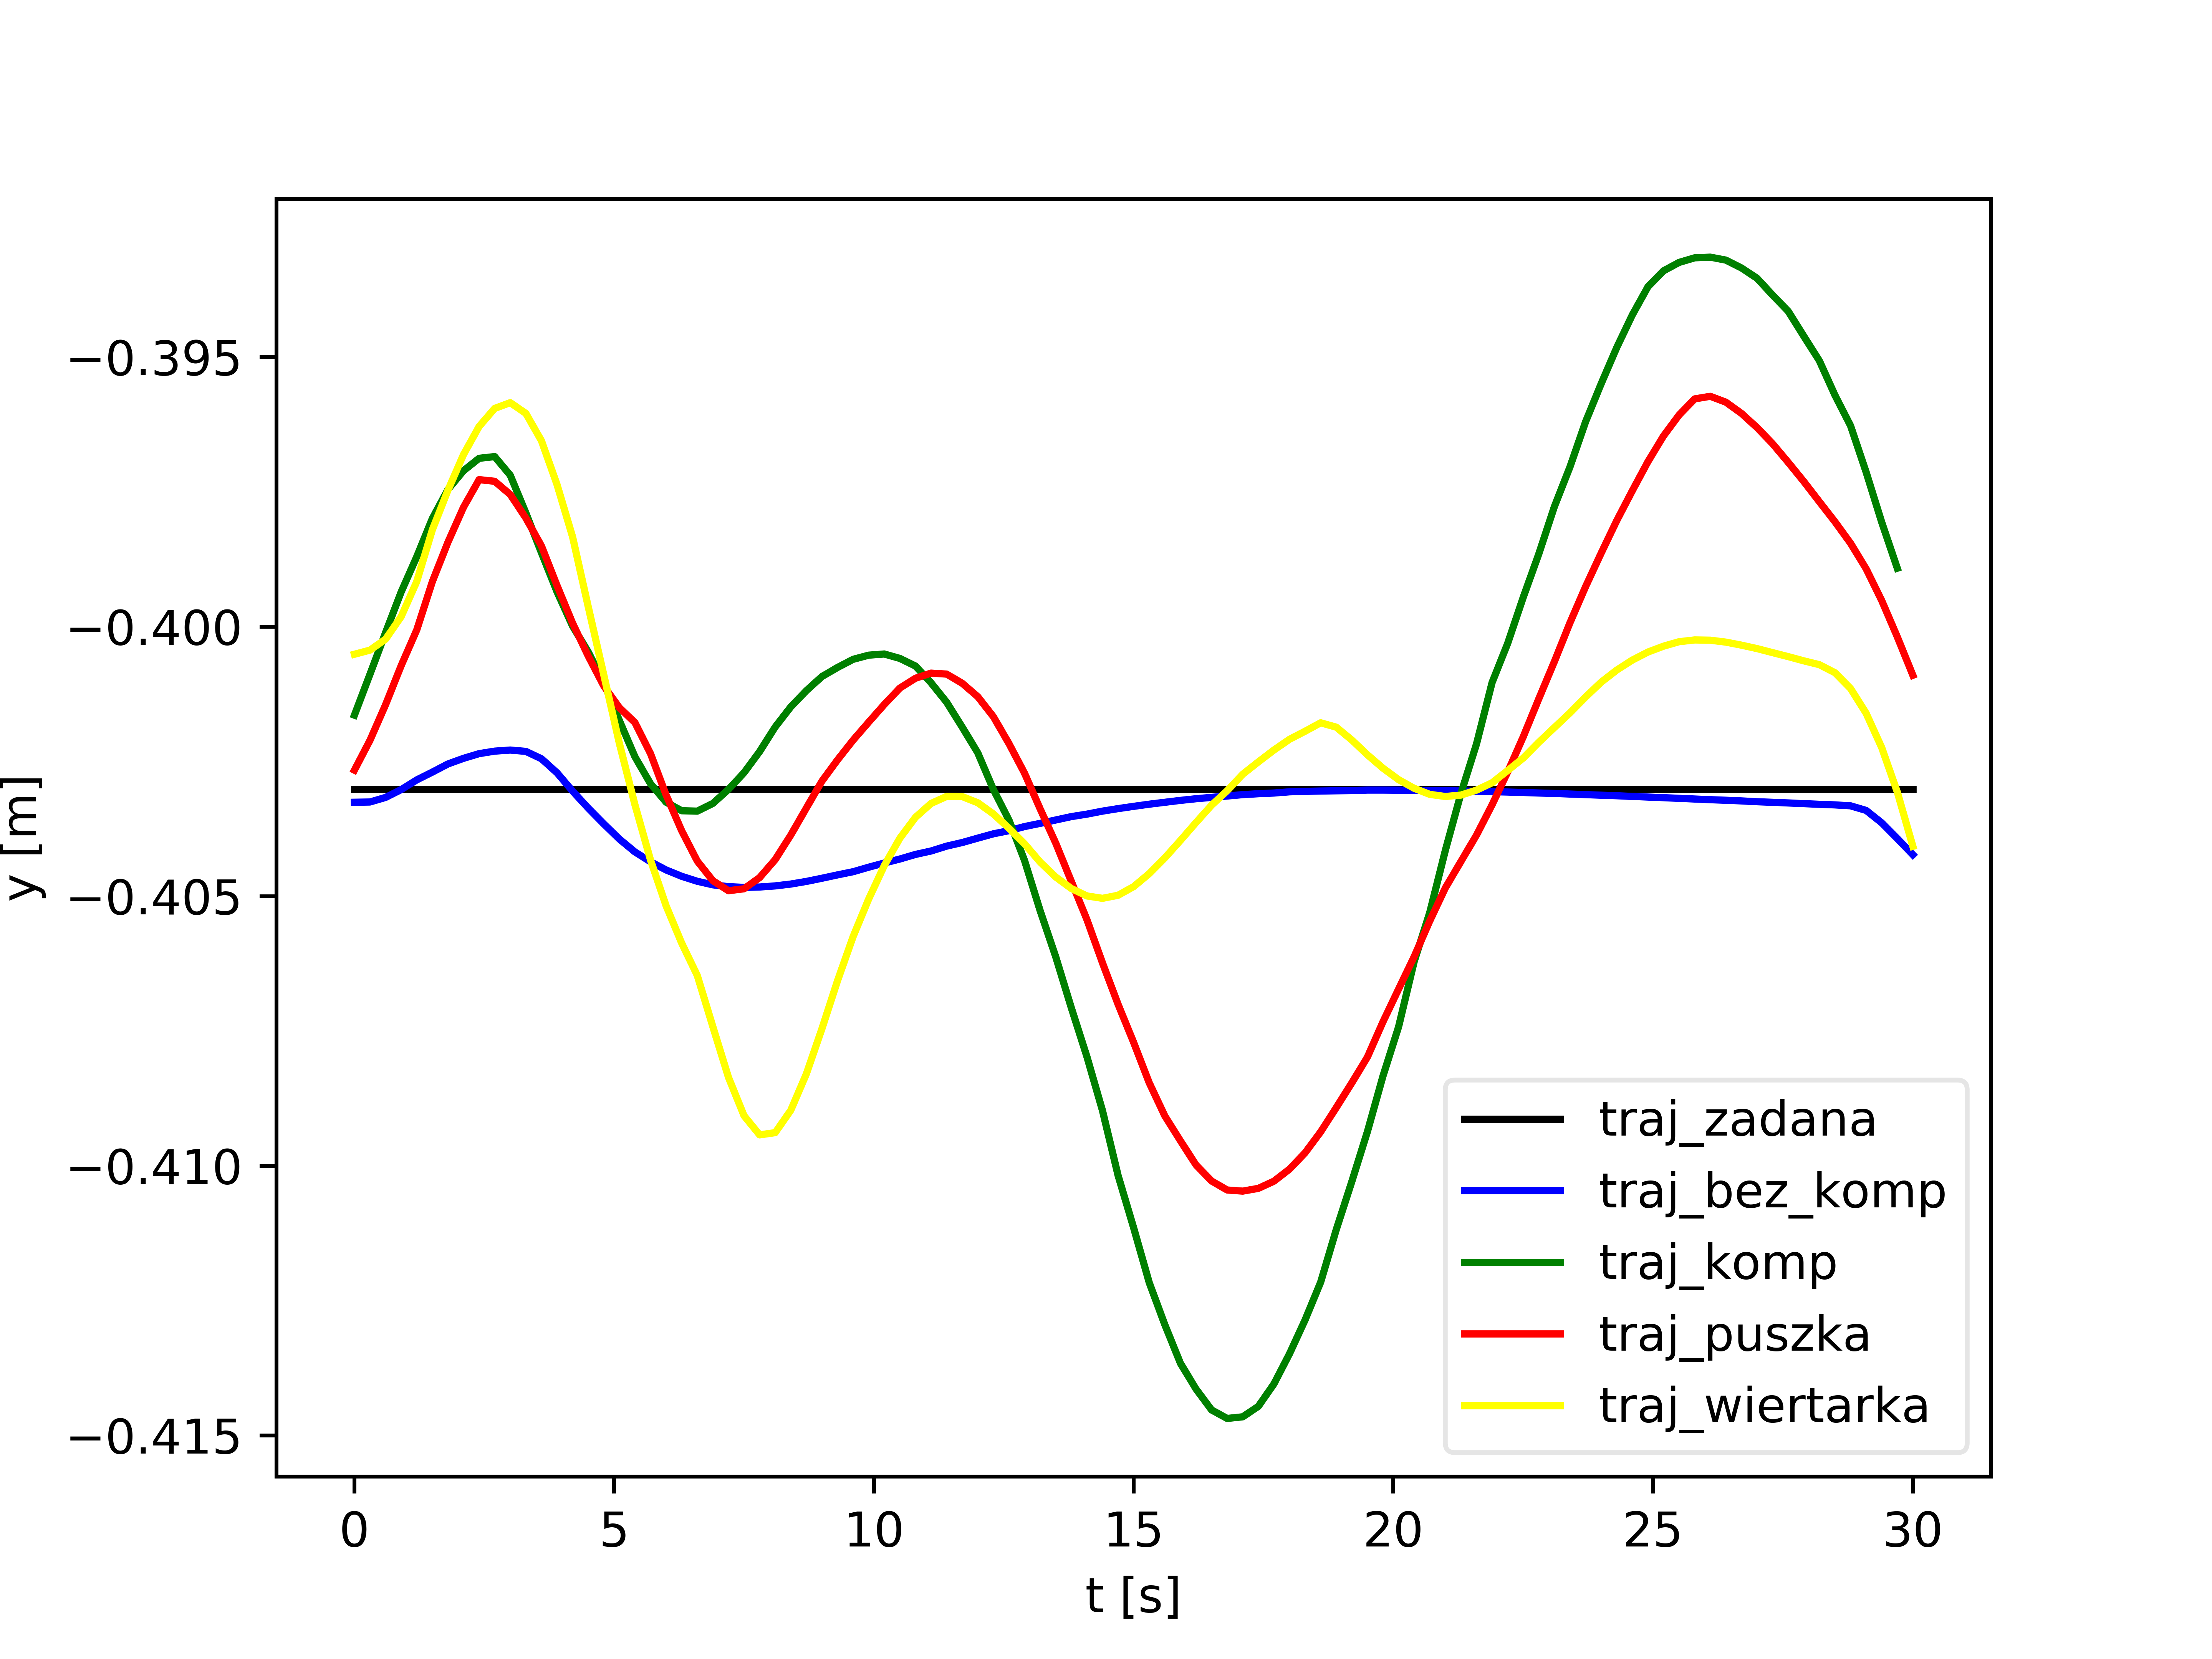
\includegraphics[width=.45\textwidth]{../../velma/przerobione_testy/out/do_gory/common_ay.png}
	}
	
	\hfill
	\subfigure[Os $Z$]{
		\label{fig:do_gory_az}
		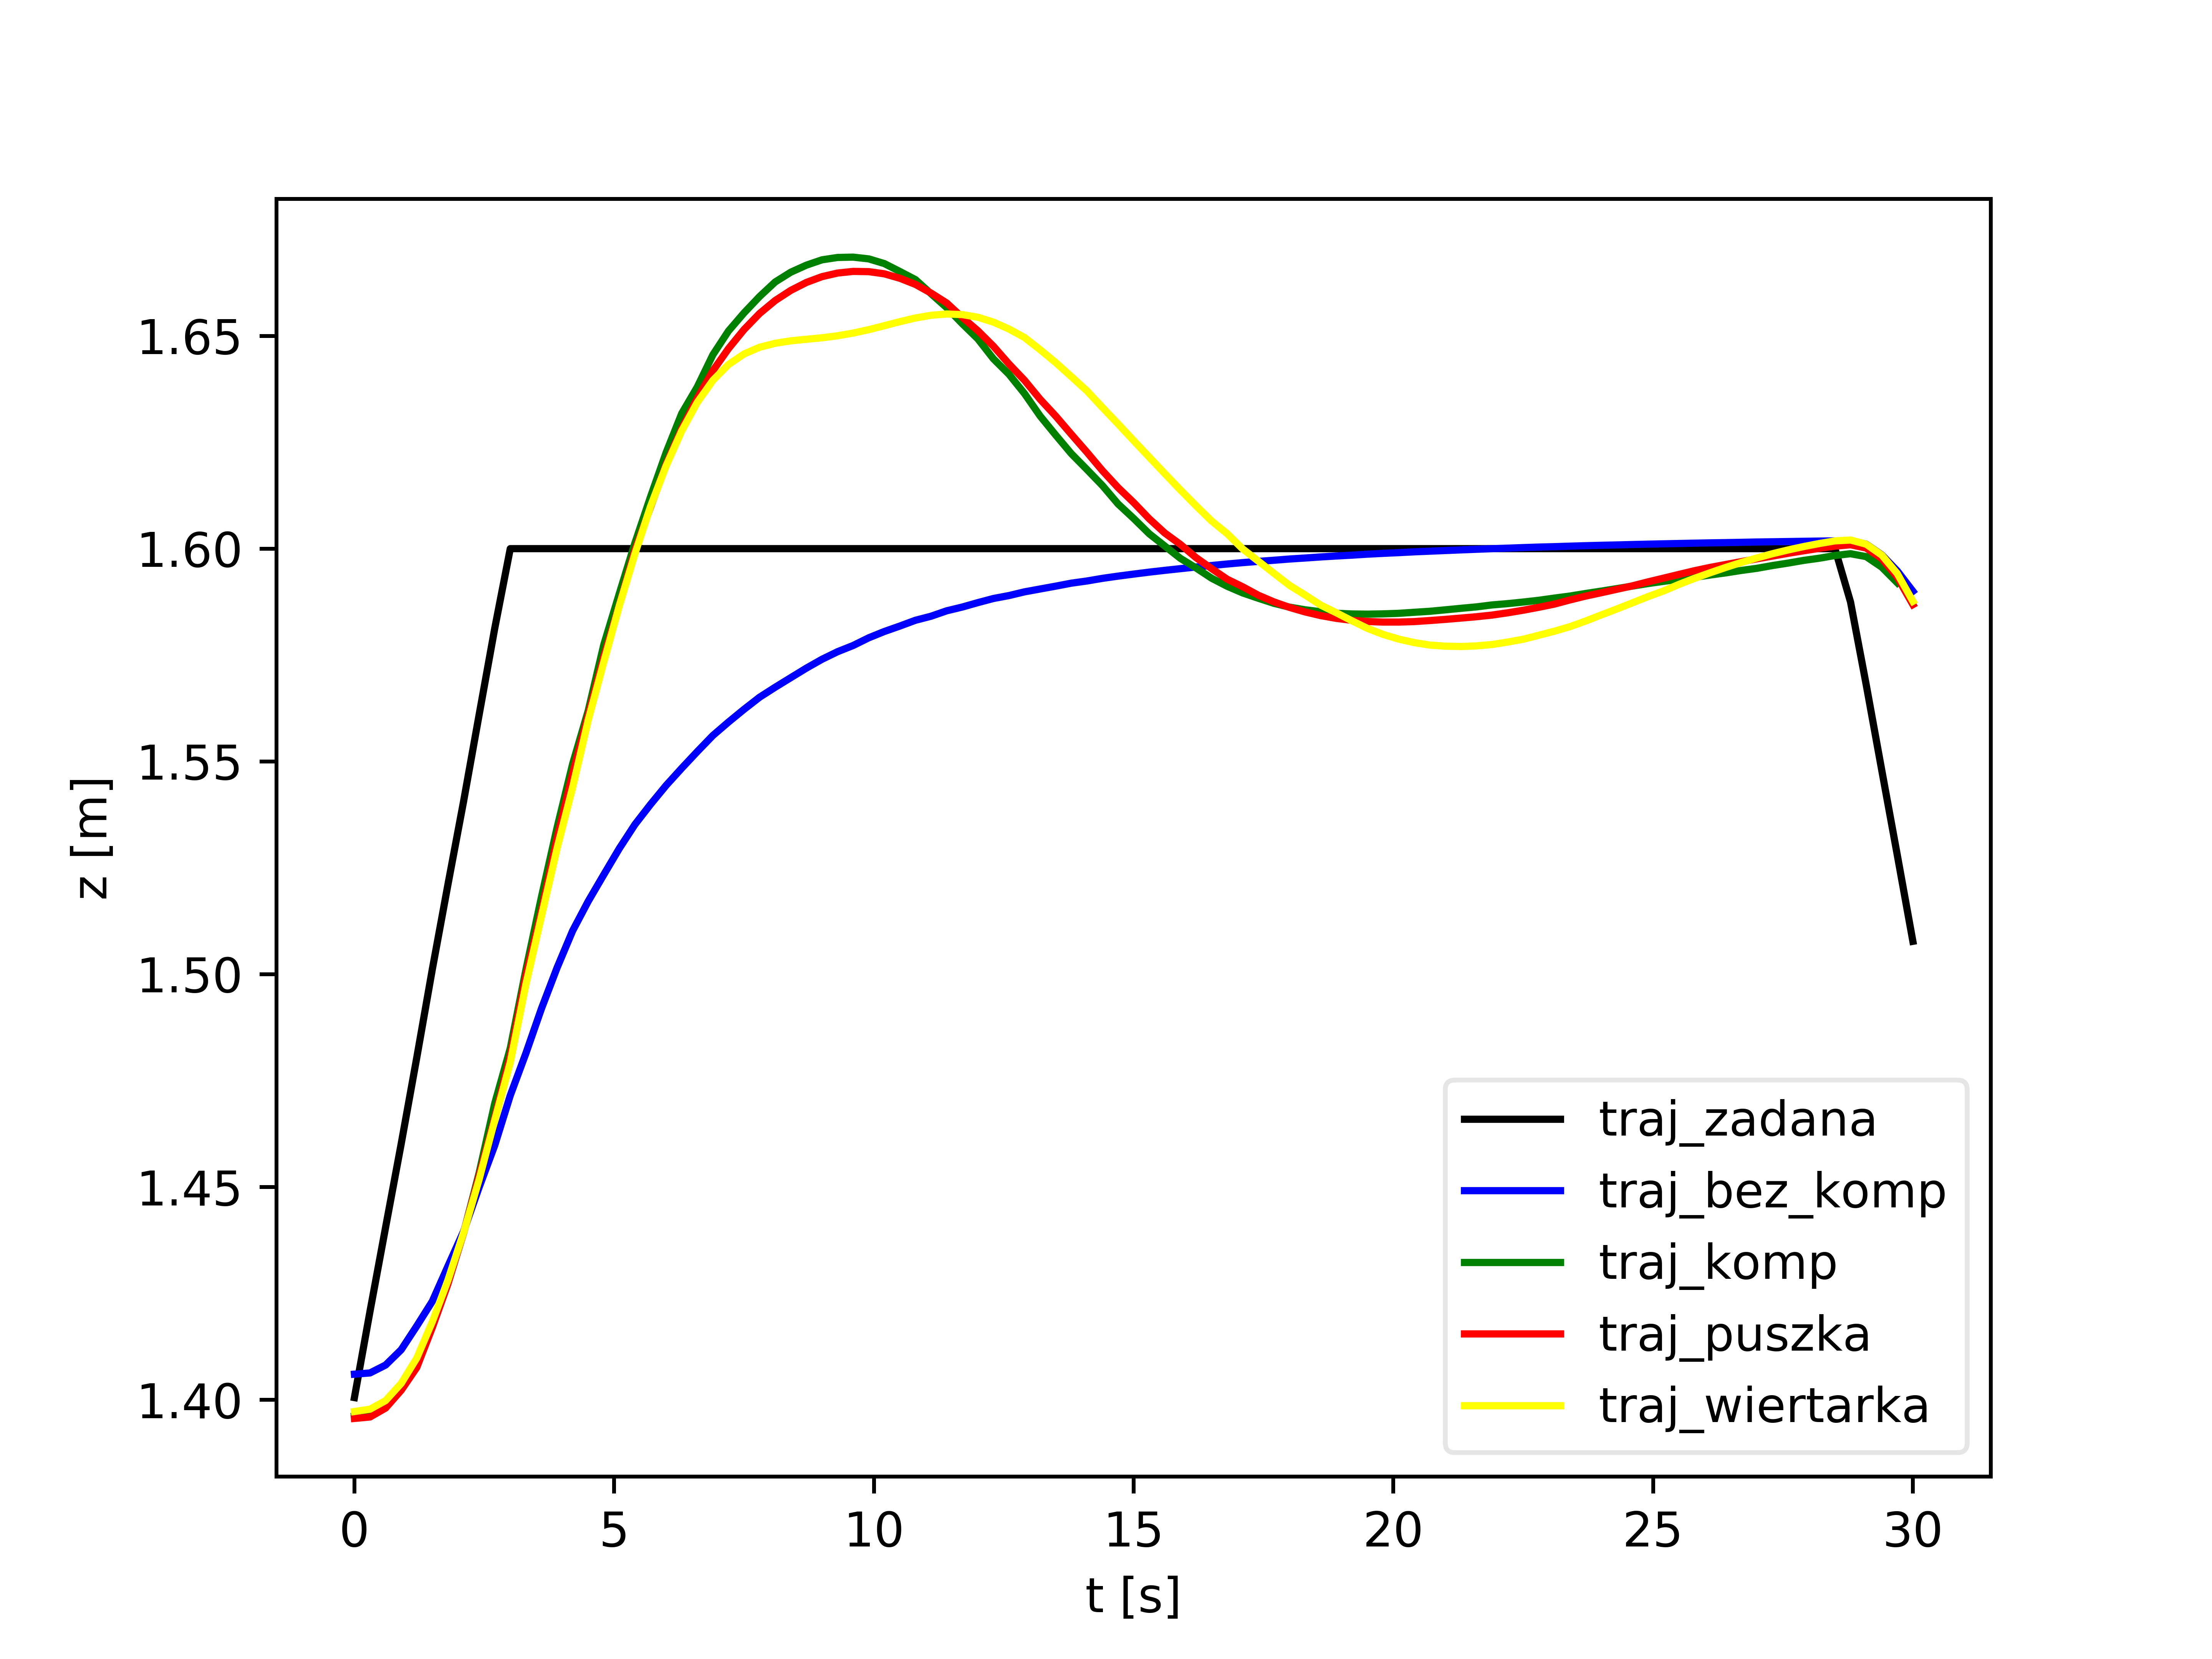
\includegraphics[width=.45\textwidth]{../../velma/przerobione_testy/out/do_gory/common_az.png}
	}

	\caption{Ruch do gory. Porownanie trajektorii pozycji w zaleznosci od czasu.}
	\label{fig:do_gory_a}

\end{figure}


\begin{figure}[h]
	\centering
	\subfigure[Kat osi $X$]{
		\label{fig:do_gory_rotx}
		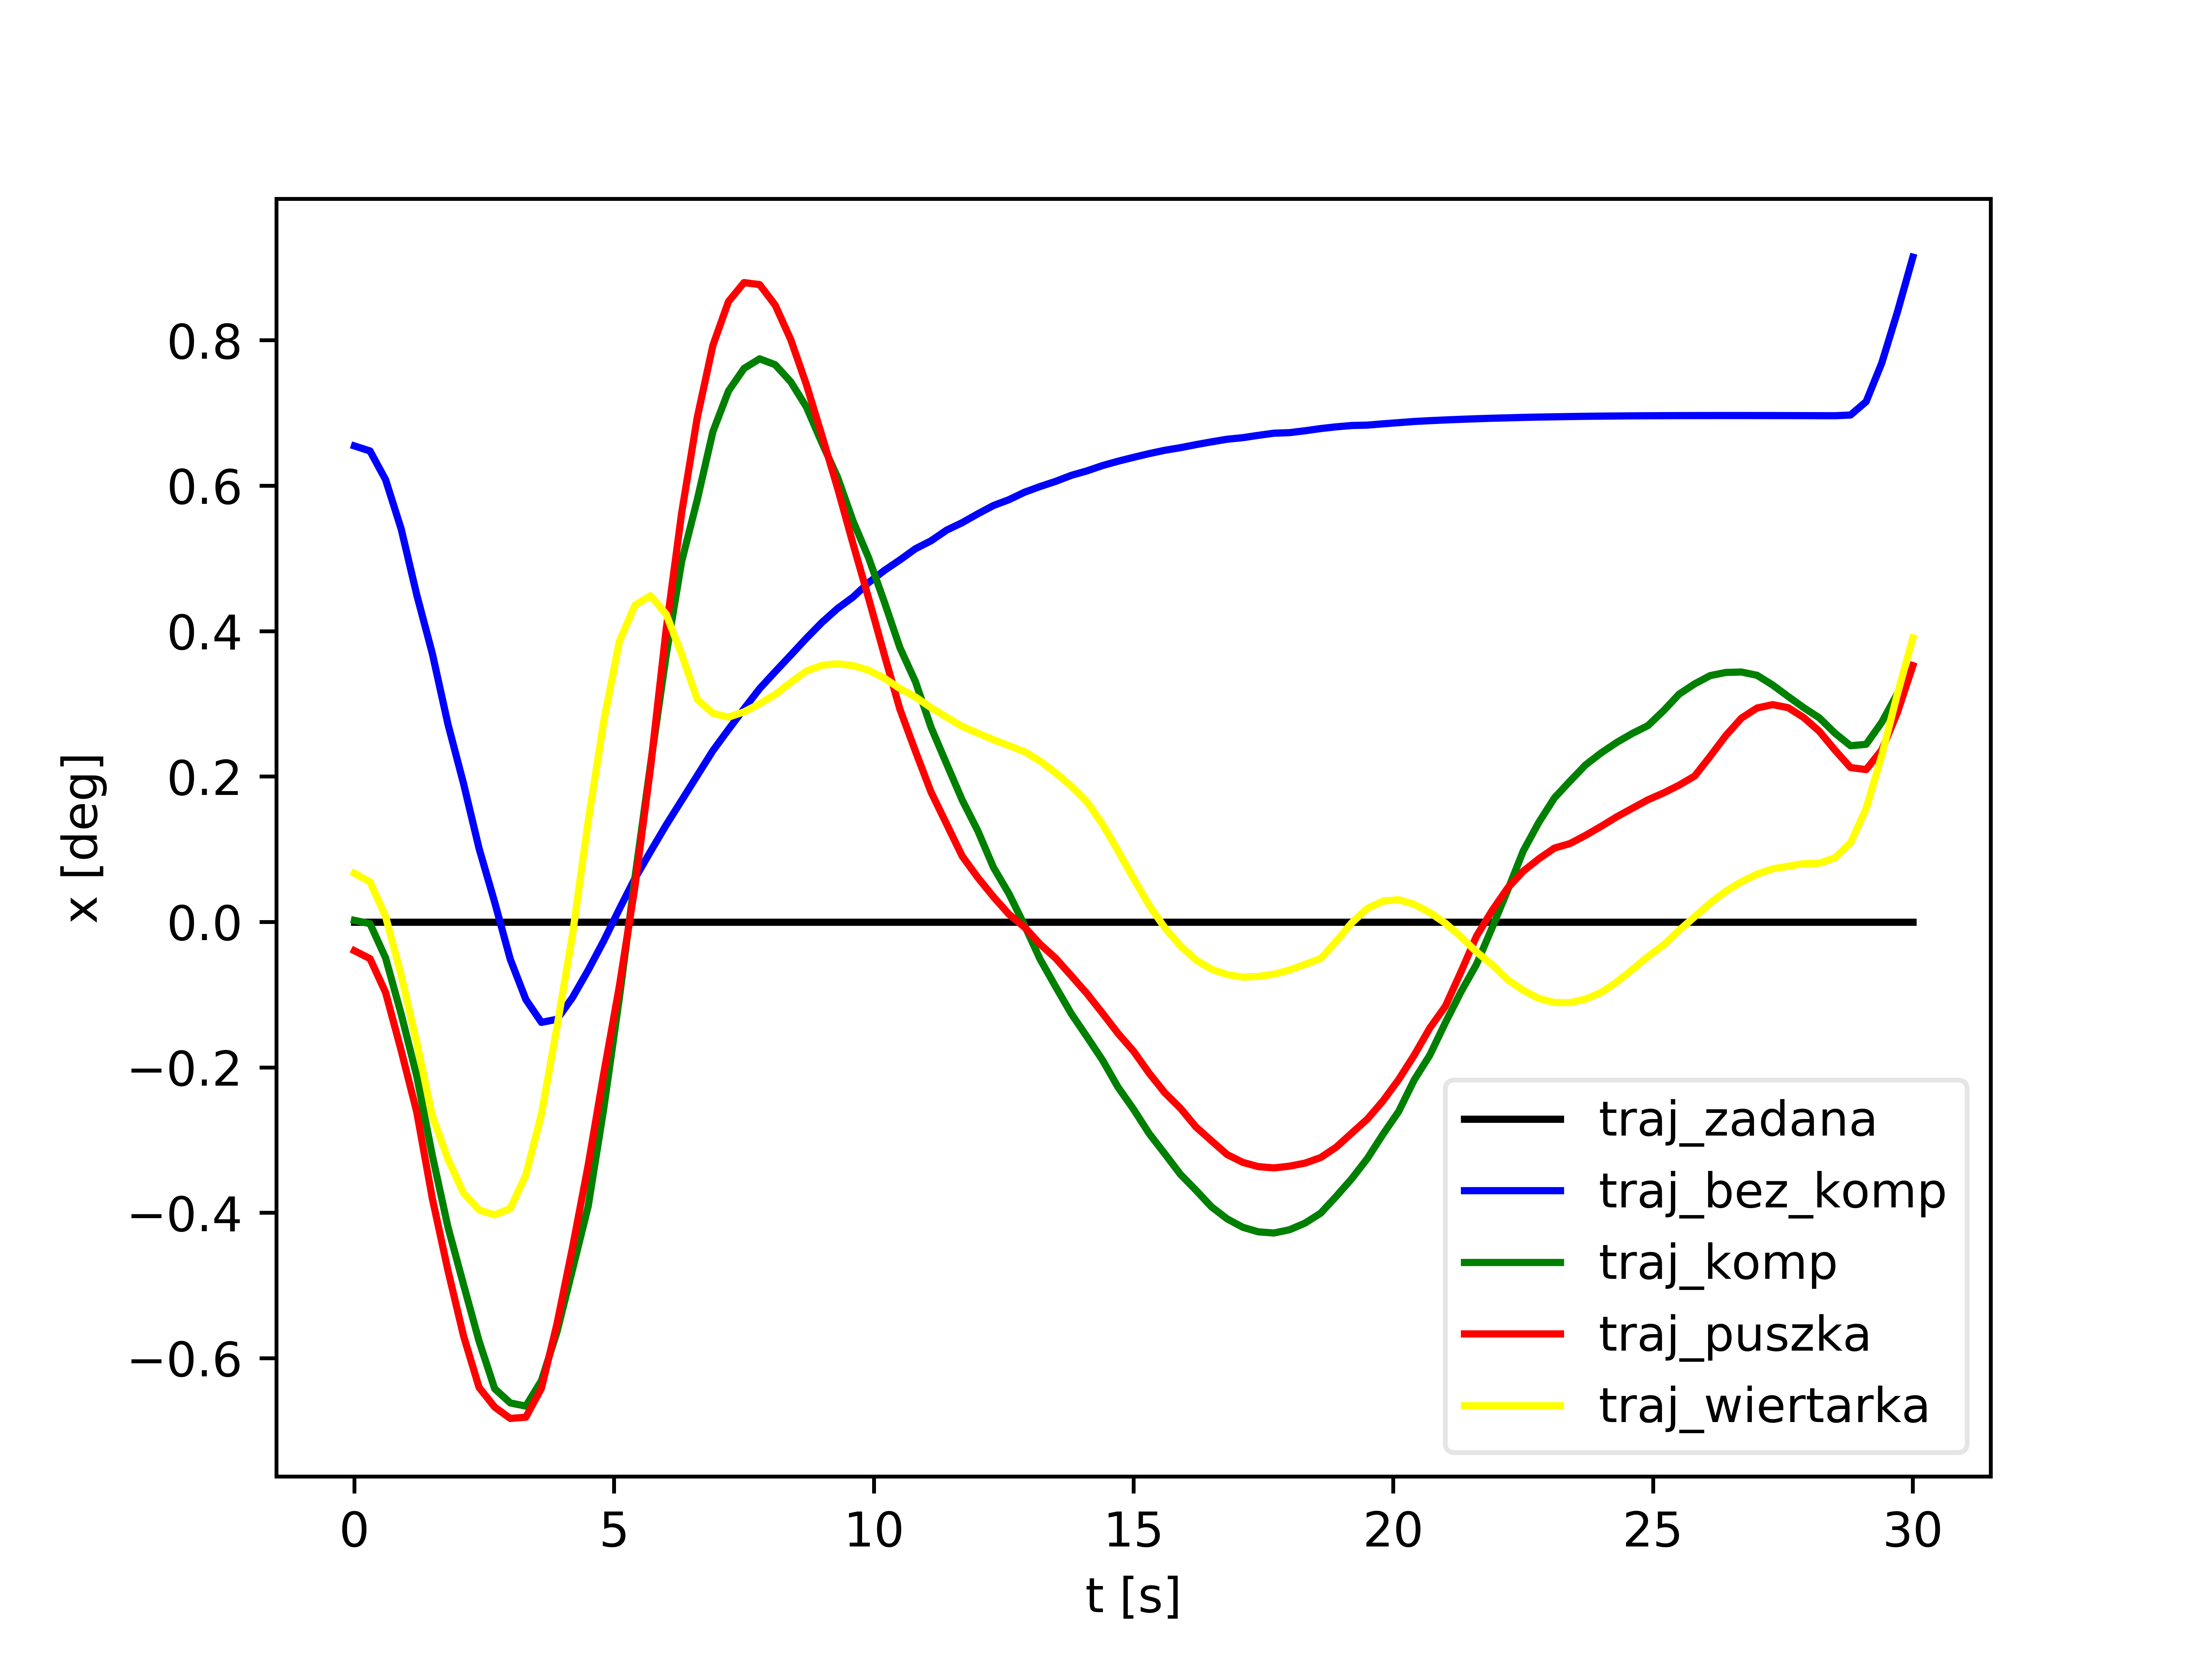
\includegraphics[width=.45\textwidth]{../../velma/przerobione_testy/out/do_gory/common_rotx.png}
	}
	\hfill
	\subfigure[Kat osi $Y$]{
		\label{fig:do_gory_roty}
		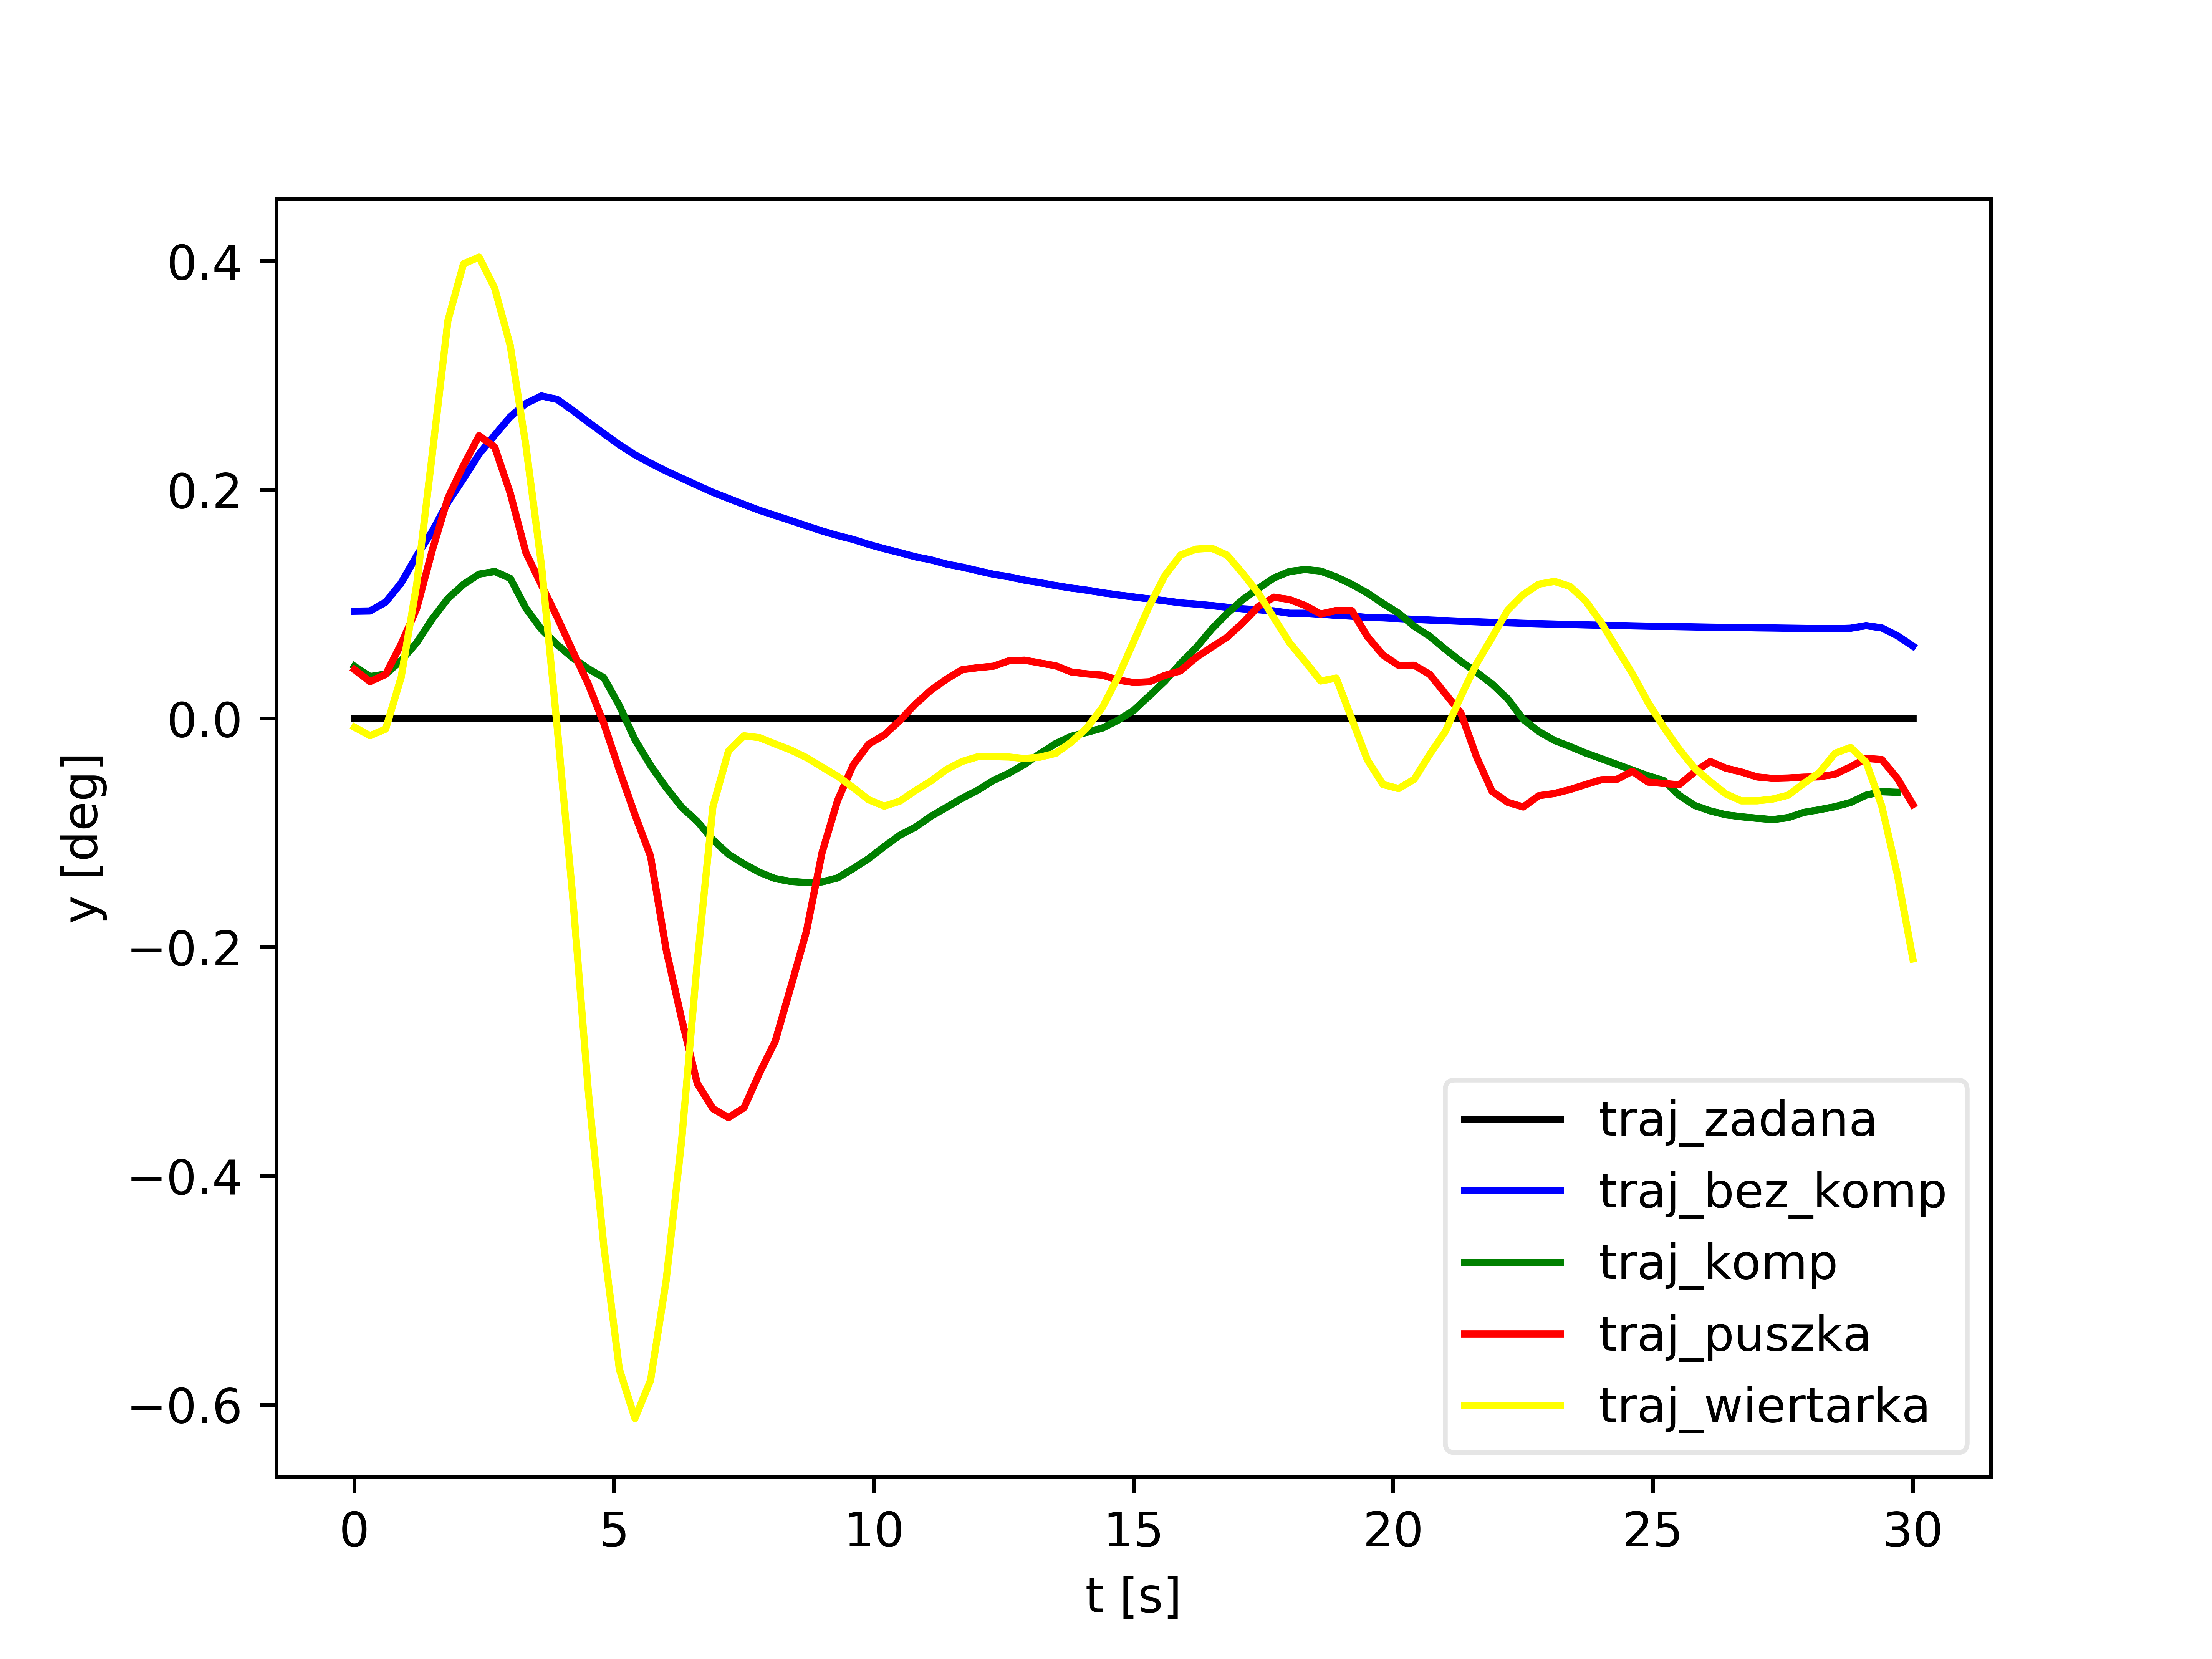
\includegraphics[width=.45\textwidth]{../../velma/przerobione_testy/out/do_gory/common_roty.png}
	}
	
	\hfill
	\subfigure[Kat osi $Z$]{
		\label{fig:do_gory_rotz}
		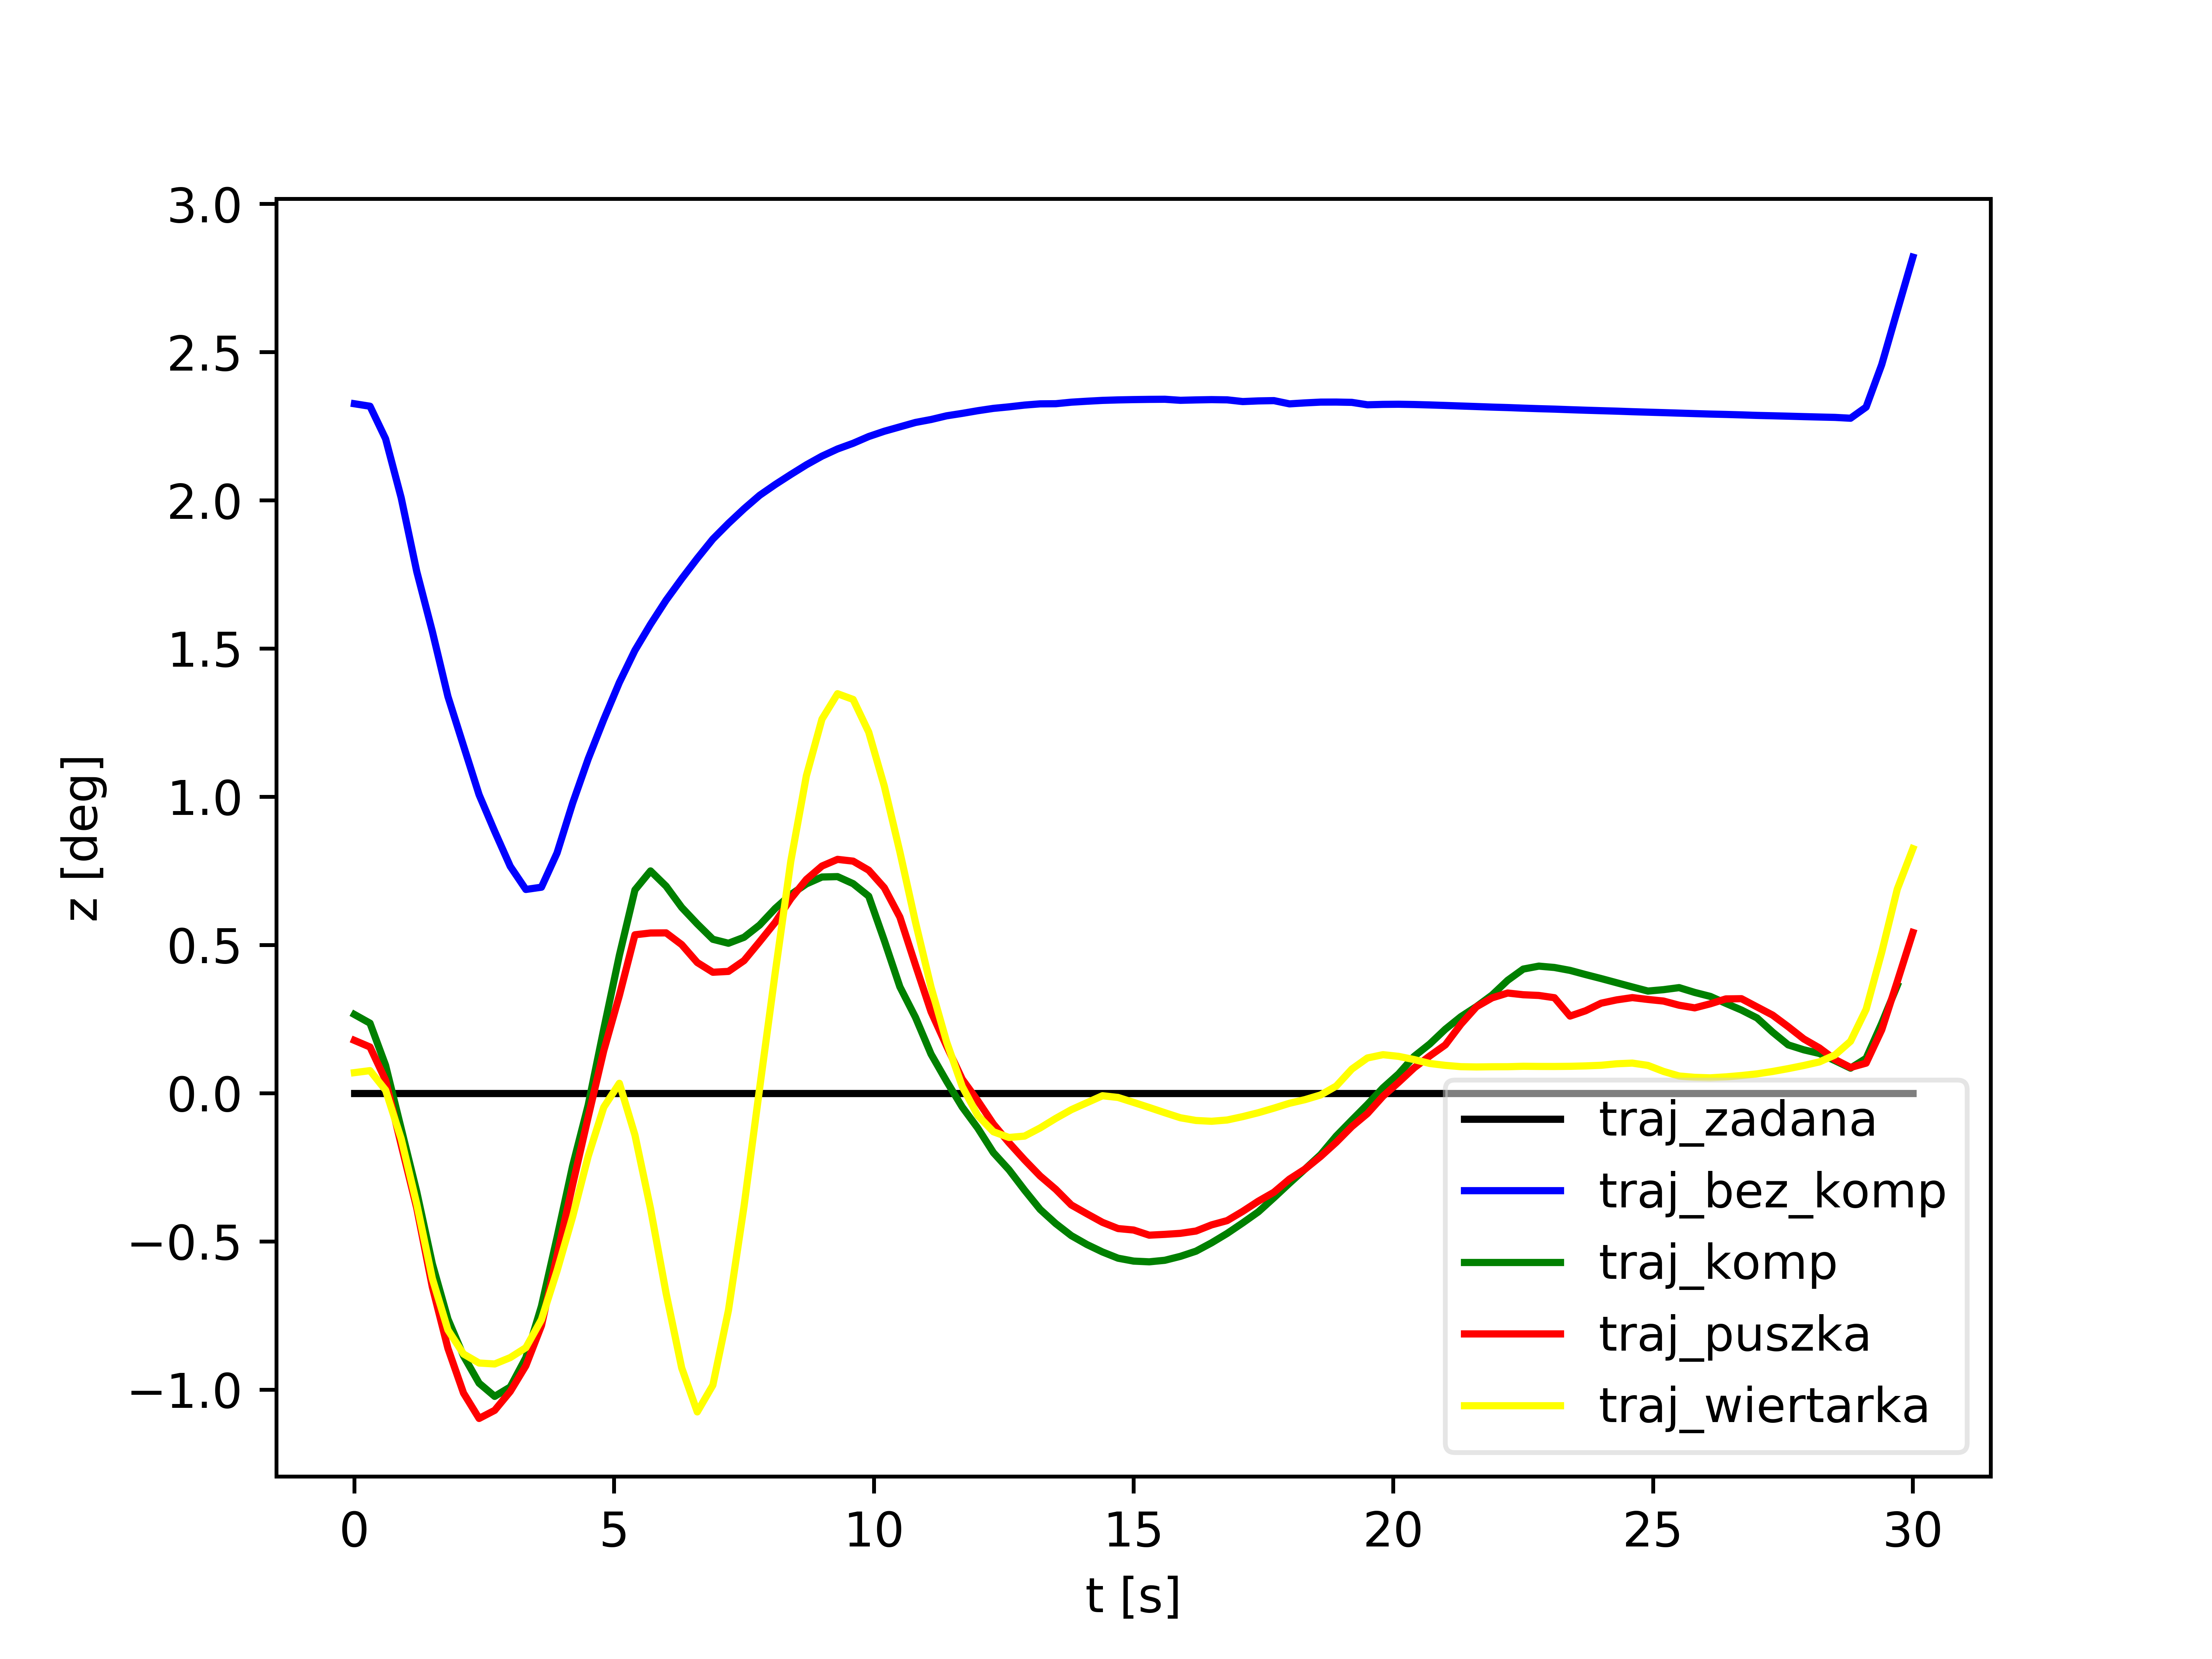
\includegraphics[width=.45\textwidth]{../../velma/przerobione_testy/out/do_gory/common_rotz.png}
	}

	\caption{Ruch do gory. Porownanie trajektorii katow w notacji Eulera w zaleznosci od czasu.}
	\label{fig:do_gory_rot}

\end{figure}


\begin{figure}[h]
	\centering
	\subfigure[Brak algorytmu kompensacji]{
		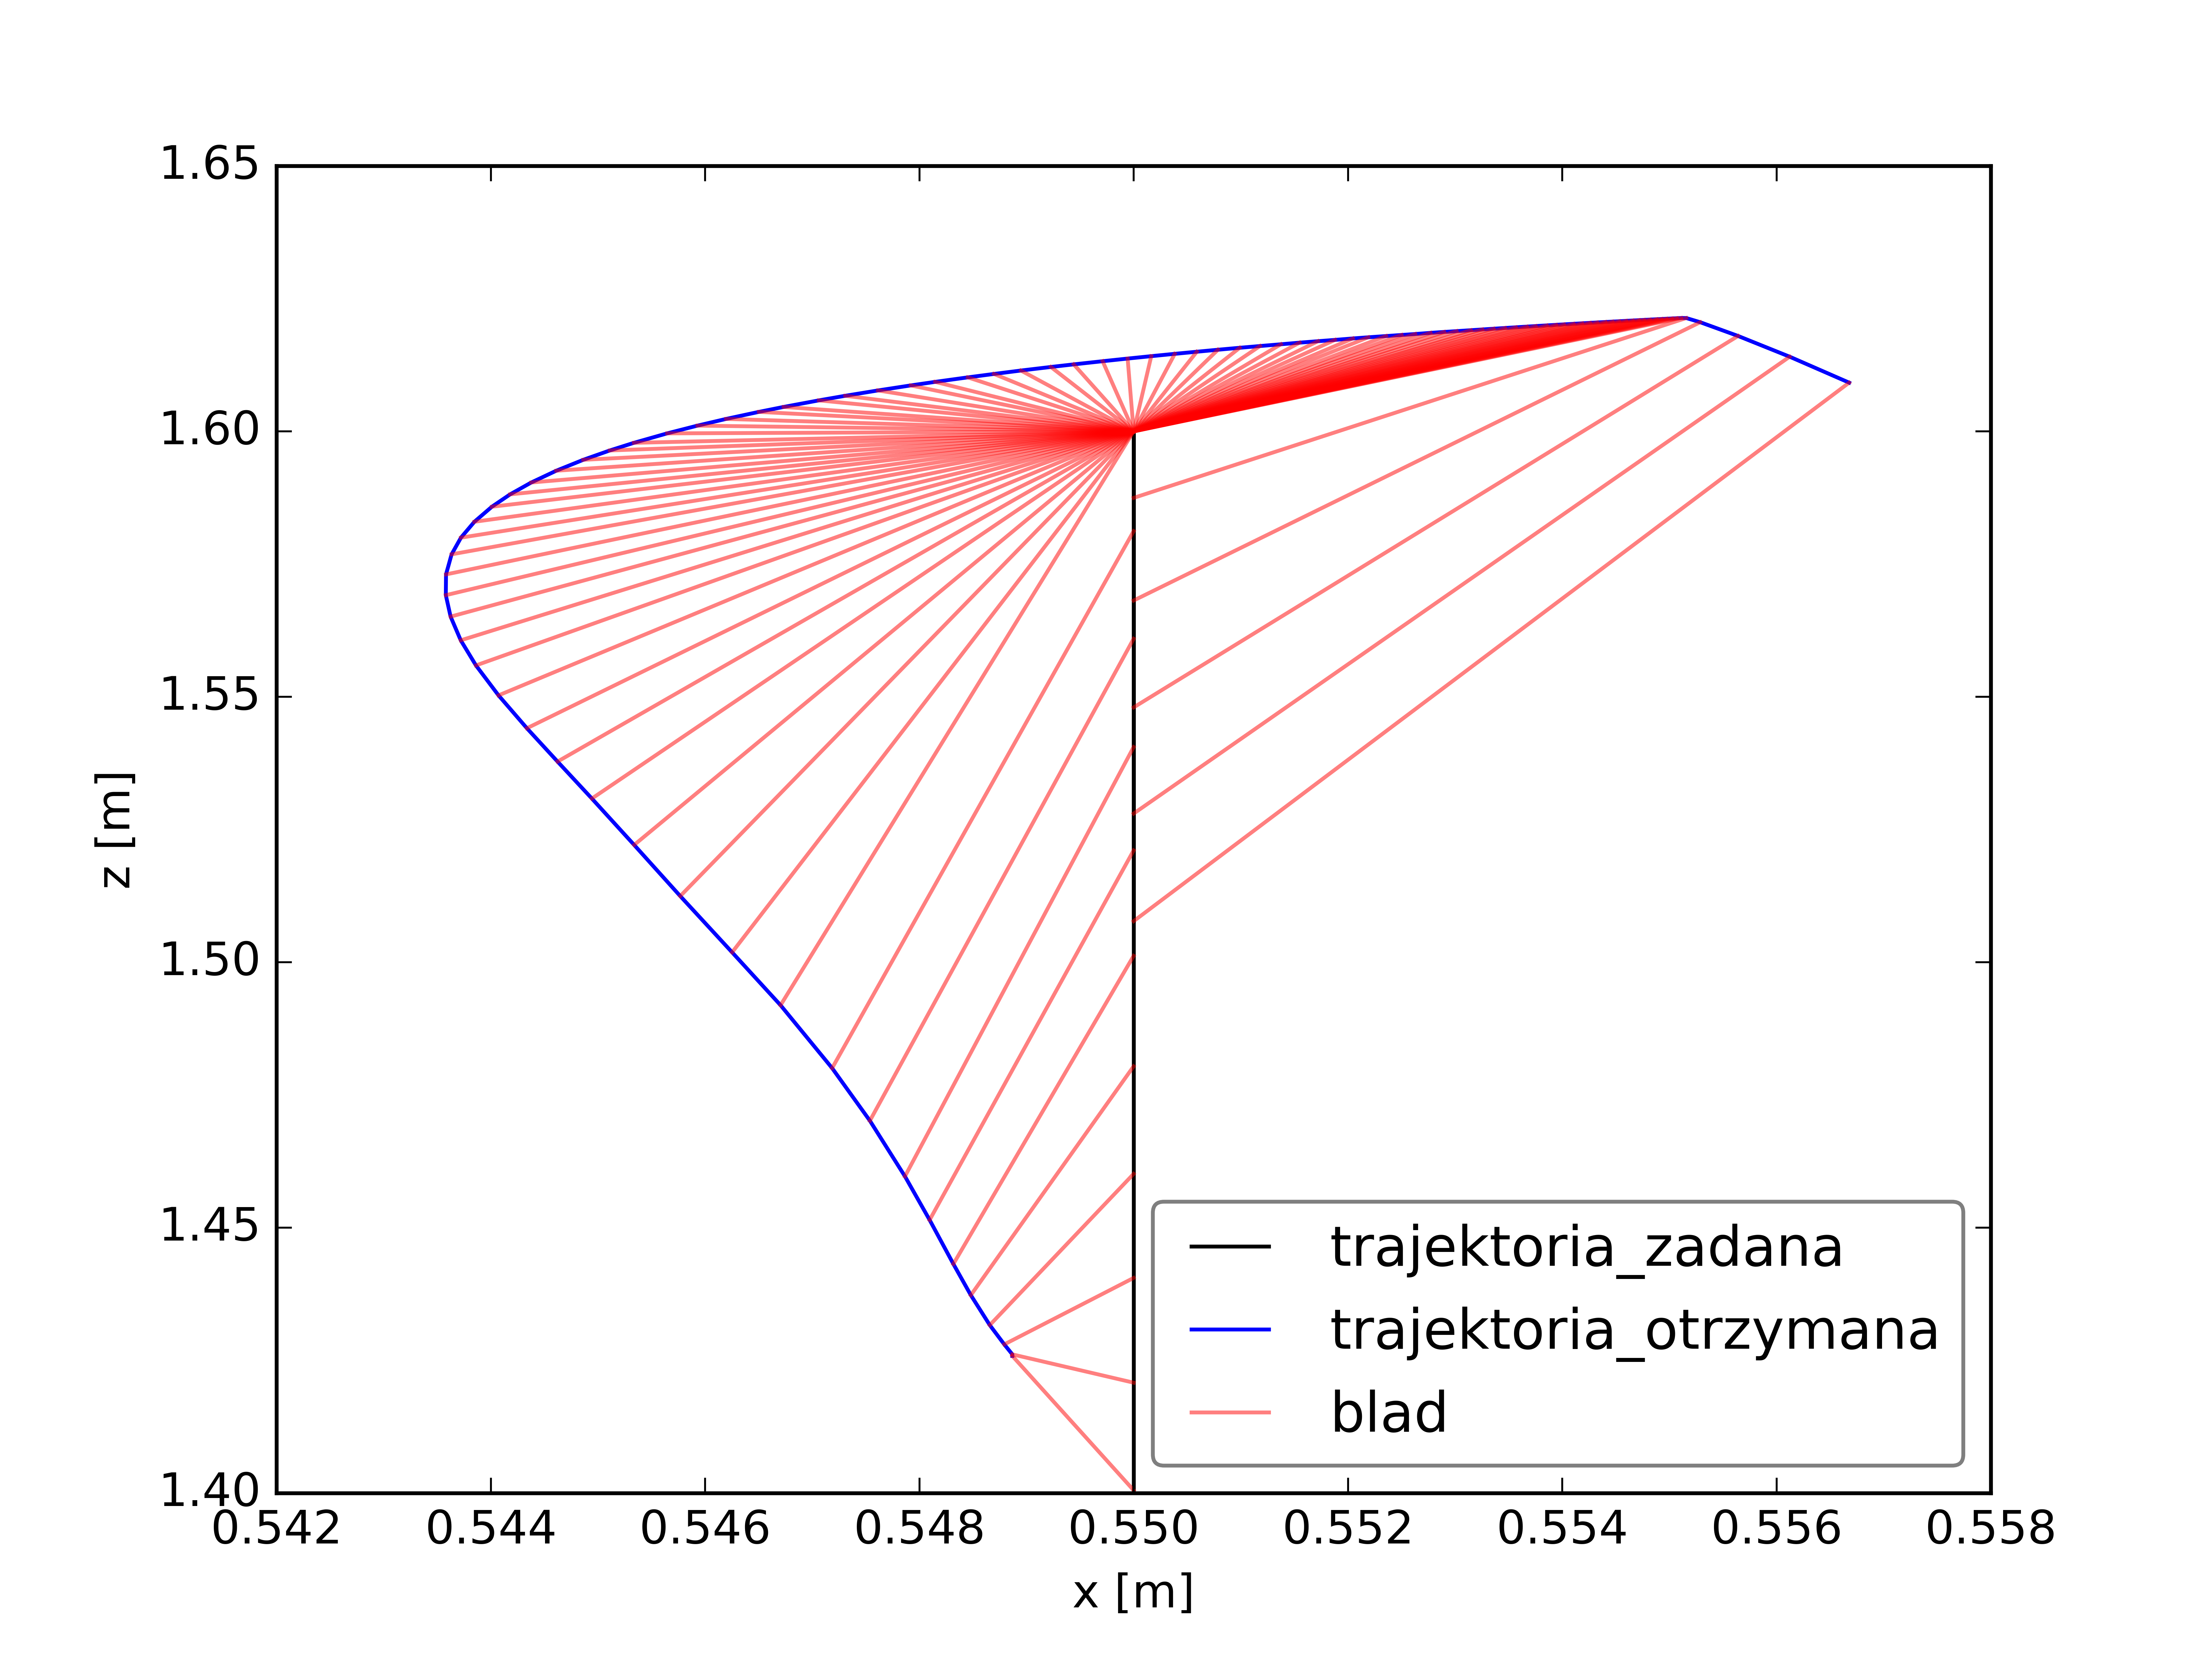
\includegraphics[width=.45\textwidth]{../../velma/przerobione_testy/out/do_gory/xz_ate_plot_podnoszenie_miekki_bez_brak.png}
	}
	\hfill
	\subfigure[Zalaczony algorytm kompnesacji]{
		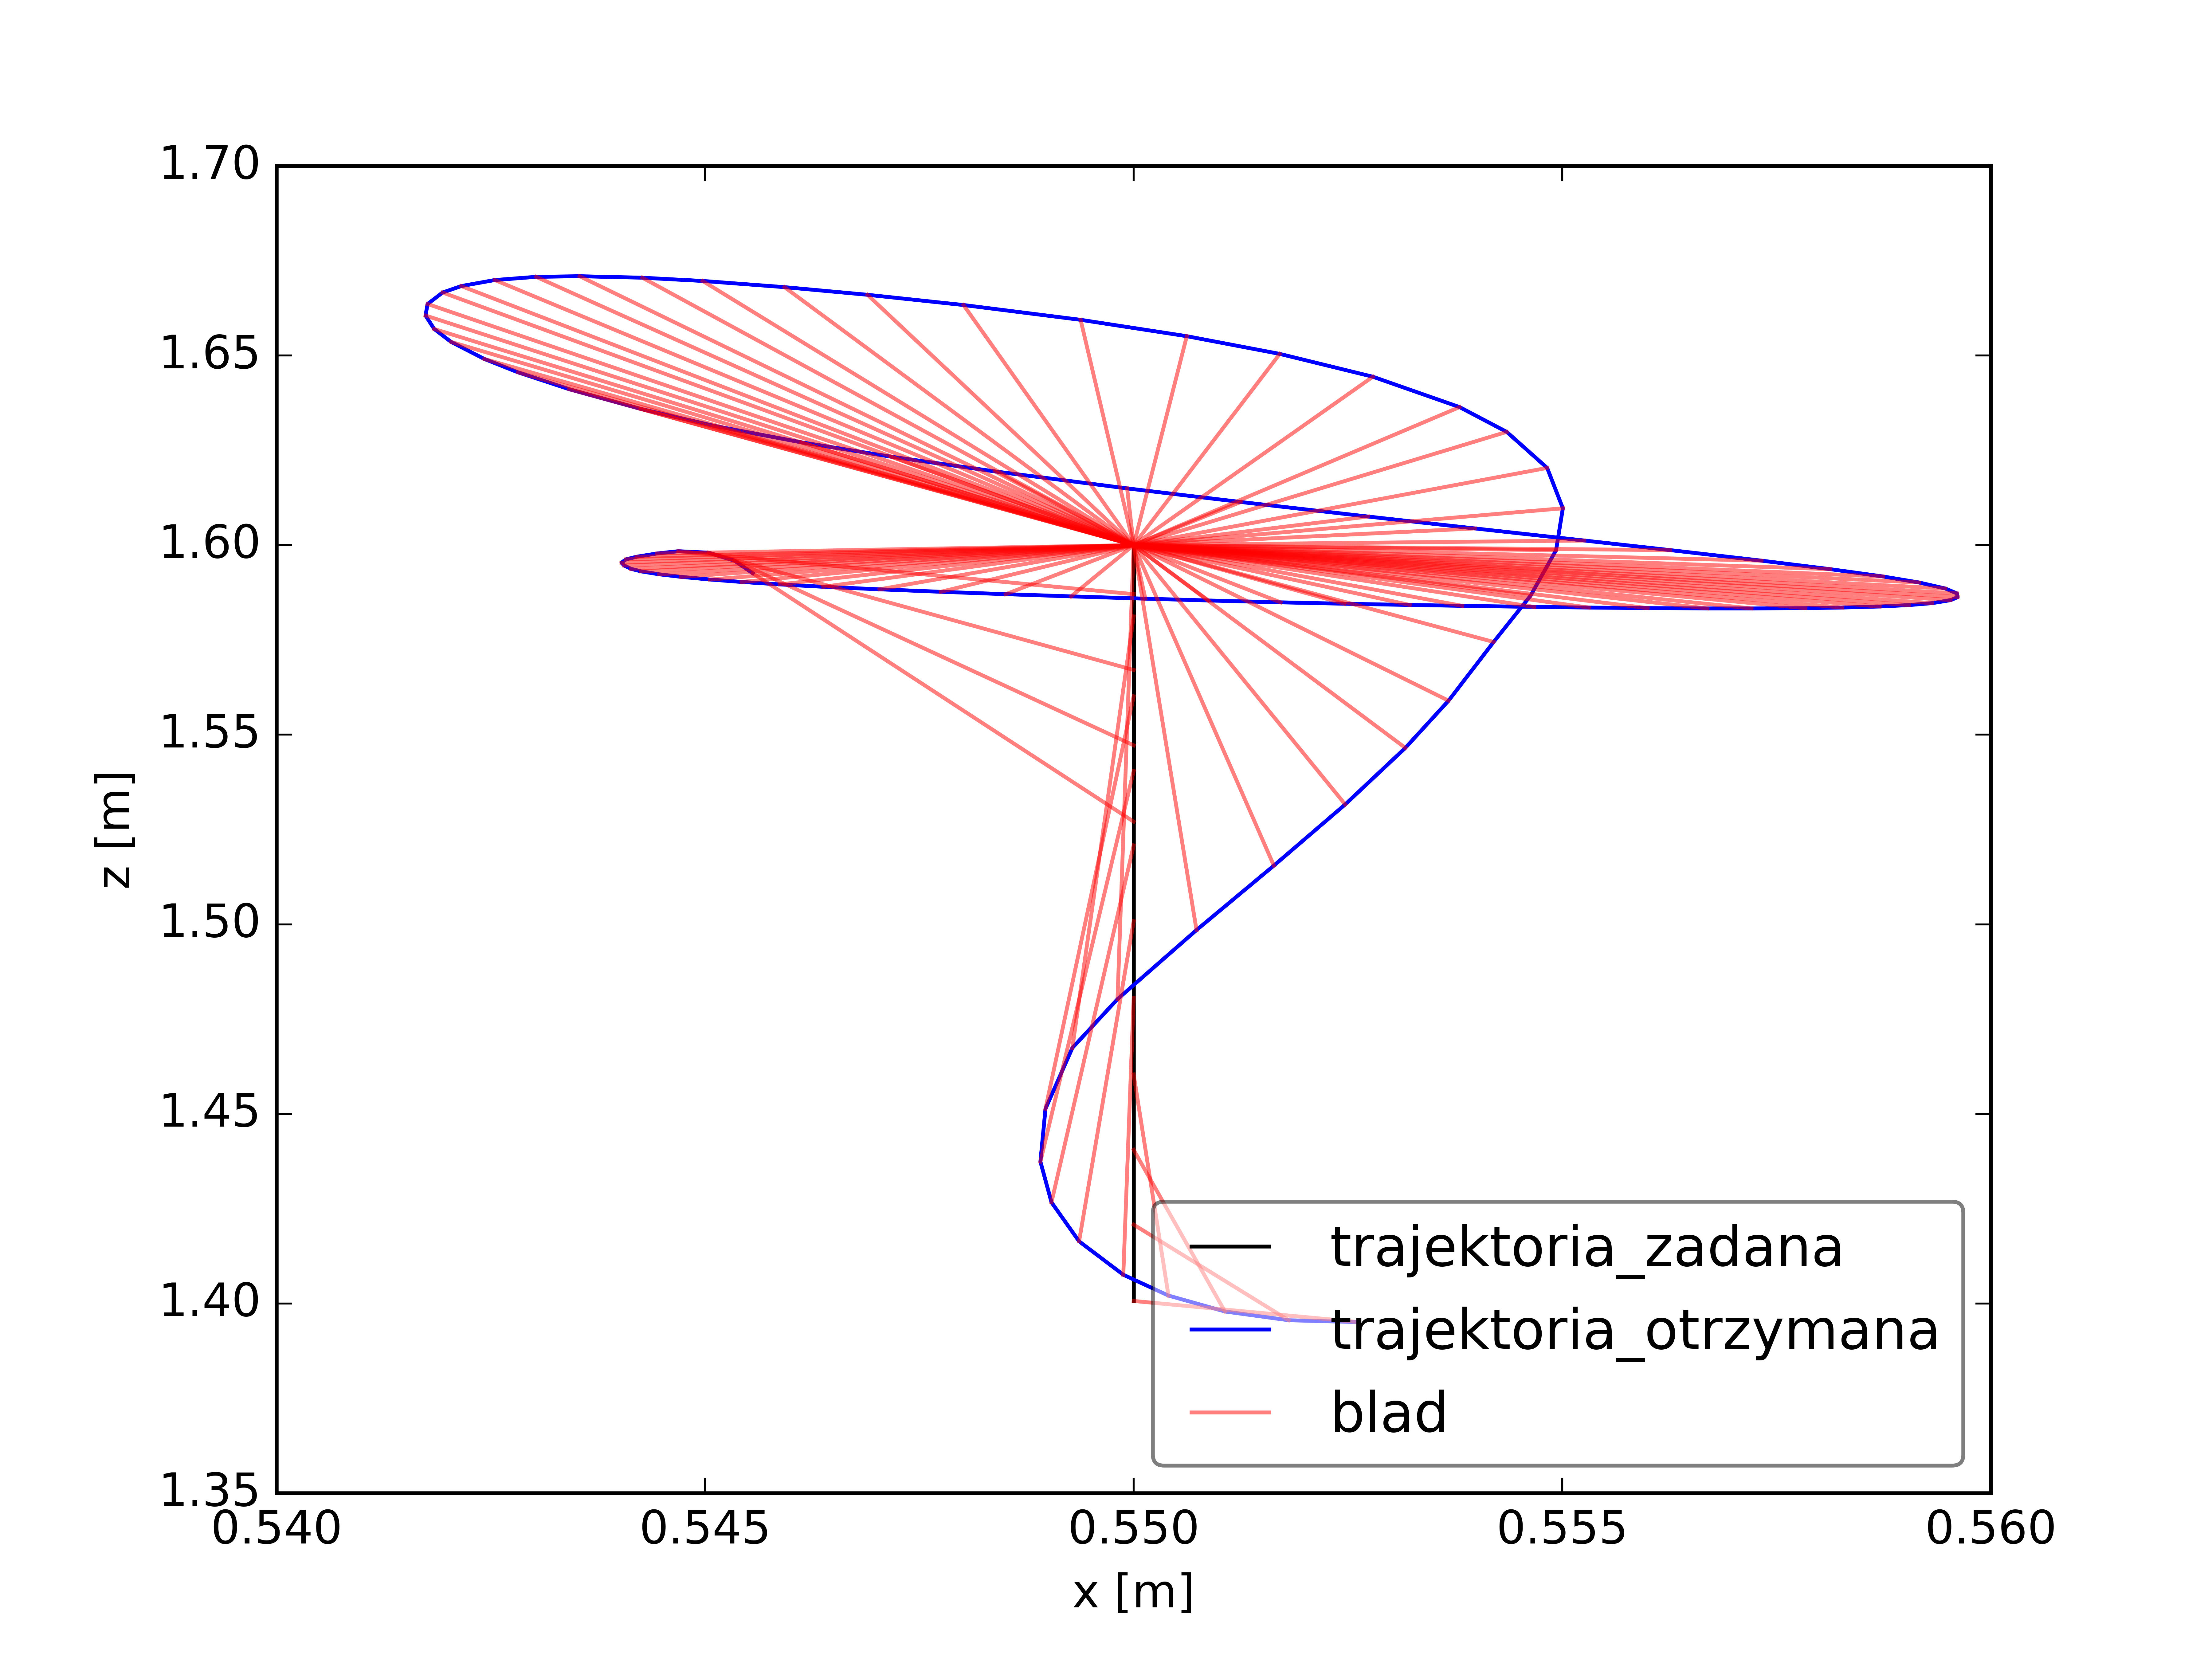
\includegraphics[width=.45\textwidth]{../../velma/przerobione_testy/out/do_gory/xz_ate_plot_podnoszenie_miekki_komp_brak.png}
	}
	\caption{Porownanie trajektorii chwytaka w osiach $X$ i $Z$}
	\label{fig:do_gory_porow_komp}
\end{figure}

\begin{figure}[h]
	\centering
	\subfigure[Trajektoria z chwycona puszka]{
		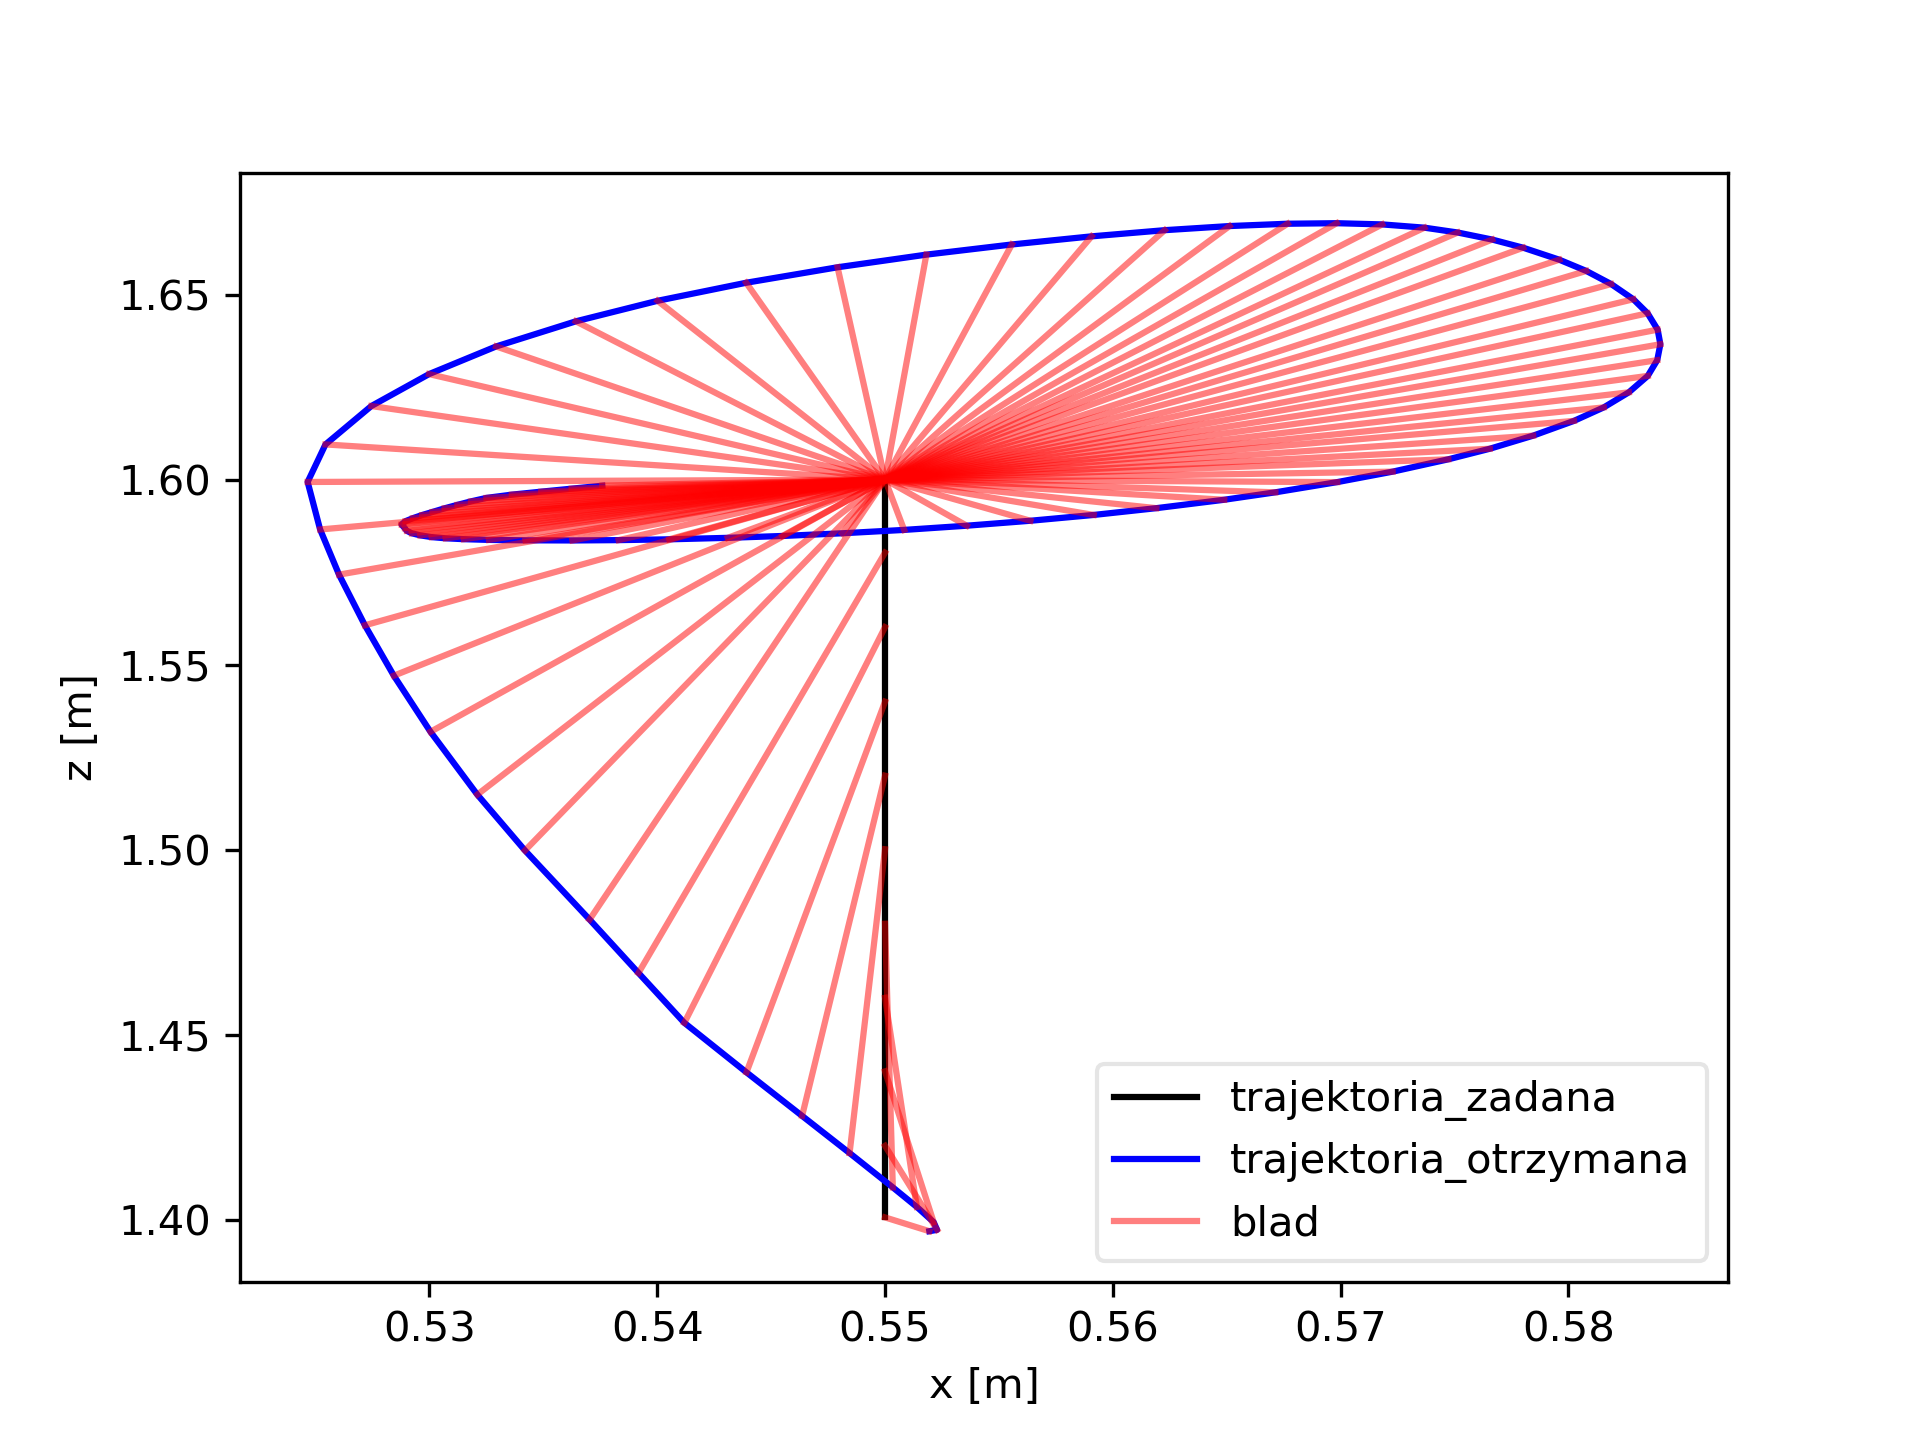
\includegraphics[width=.45\textwidth]{../../velma/przerobione_testy/out/do_gory/xz_ate_plot_podnoszenie_miekki_komp_piwo.png}
	}
	\hfill
	\subfigure[Trajektoria z chwycona wiertarka]{
		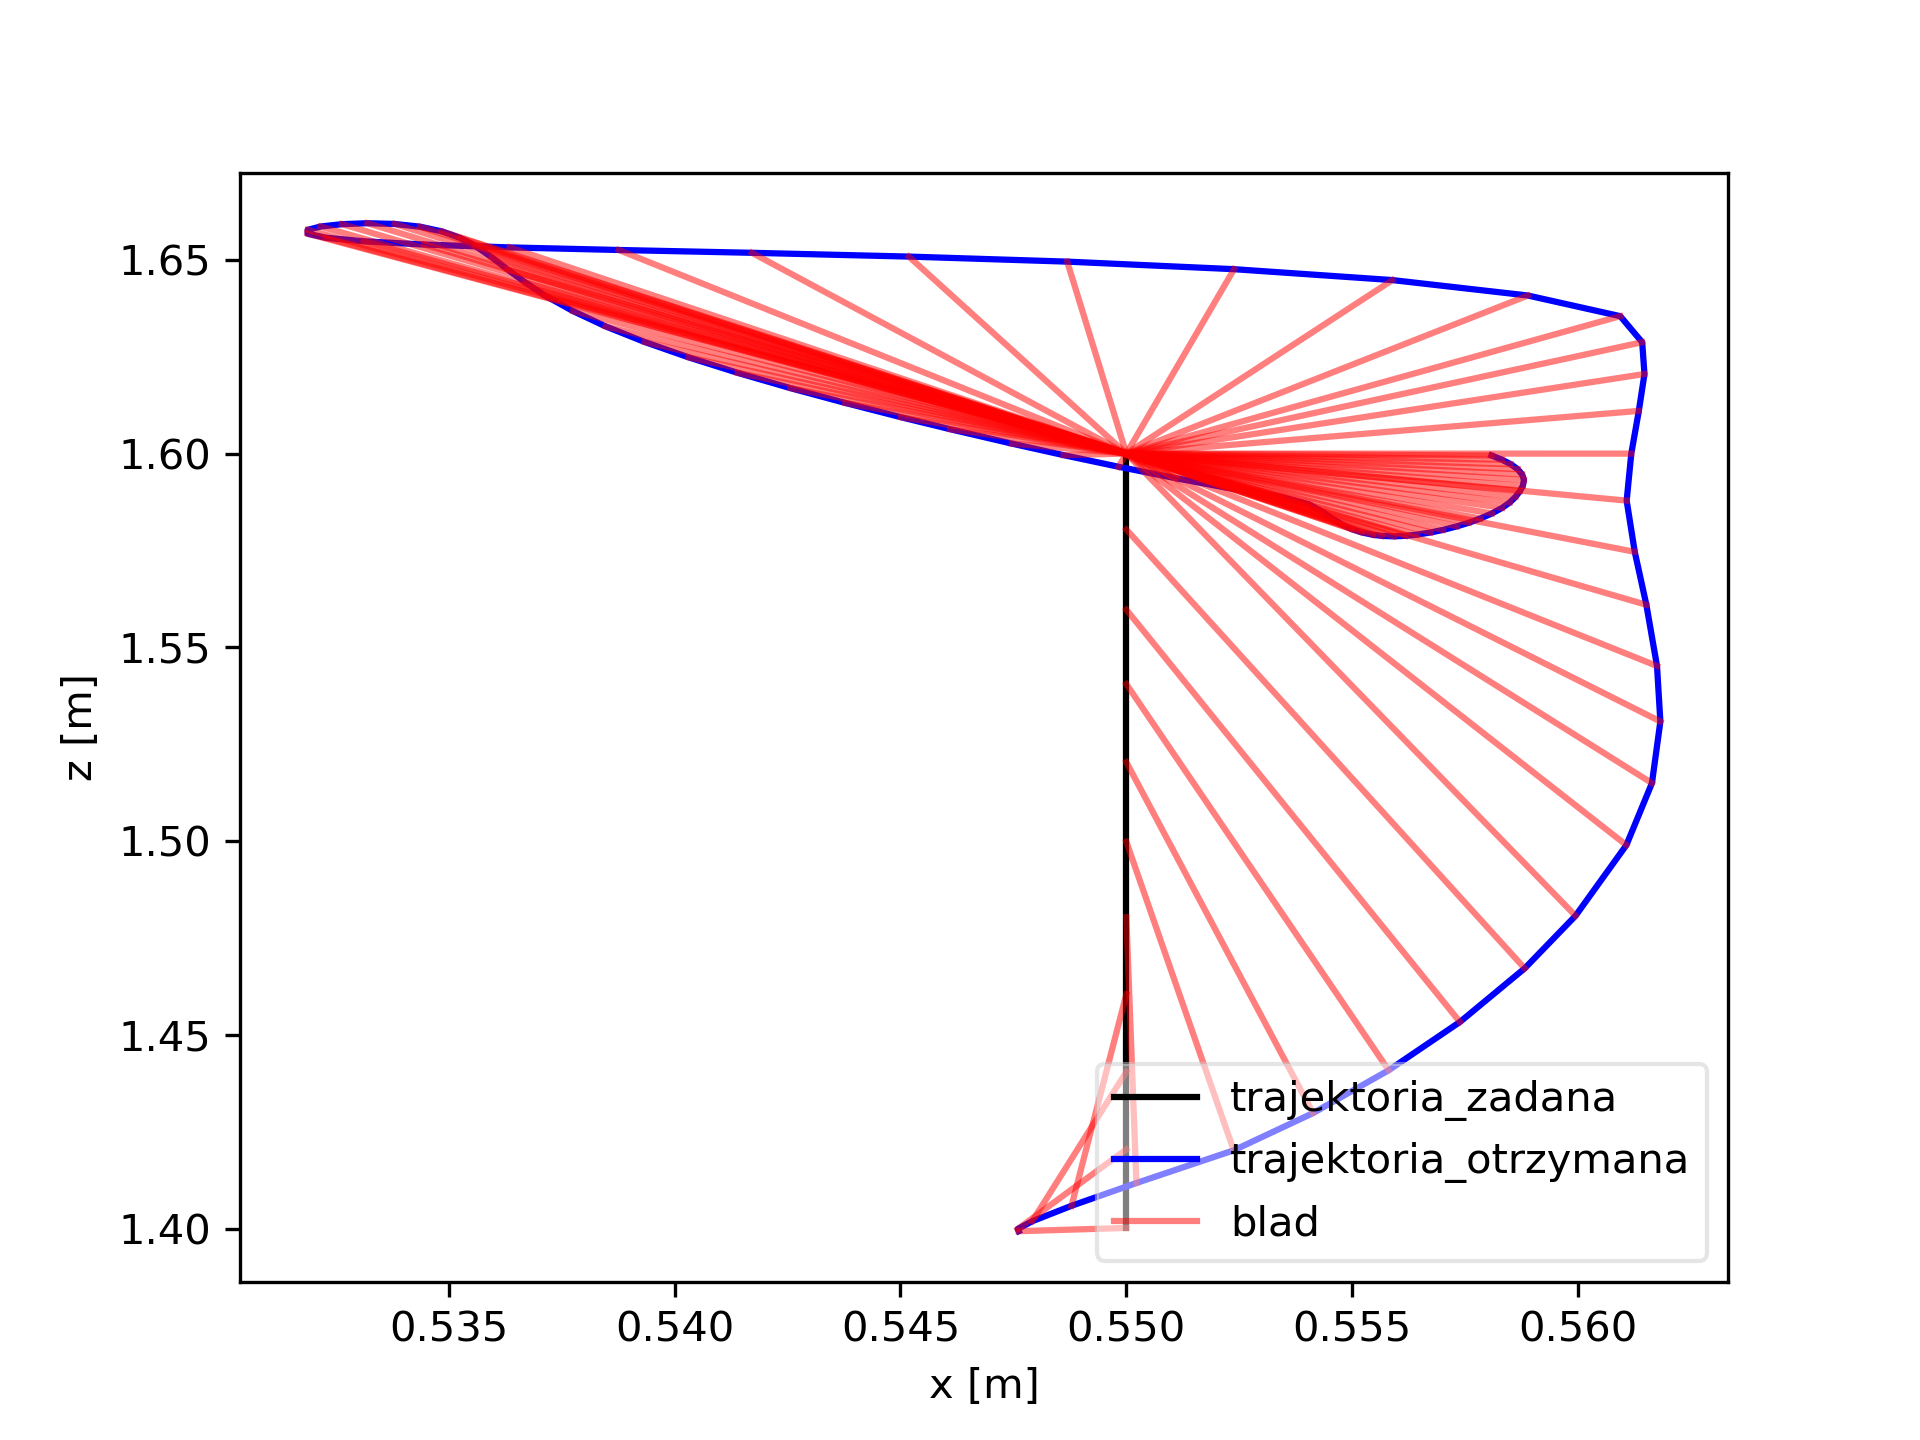
\includegraphics[width=.45\textwidth]{../../velma/przerobione_testy/out/do_gory/xz_ate_plot_podnoszenie_miekki_komp_wiertarka.png}
	}
	\caption{Porownanie trajektorii chwytaka w osiach $X$ i $Z$}
	\label{fig:do_gory_porow_przedm}
\end{figure}


% \begin{figure}
% 	\centering
% 	\subfigure[Brak algorytmu kompensacji]{
% 		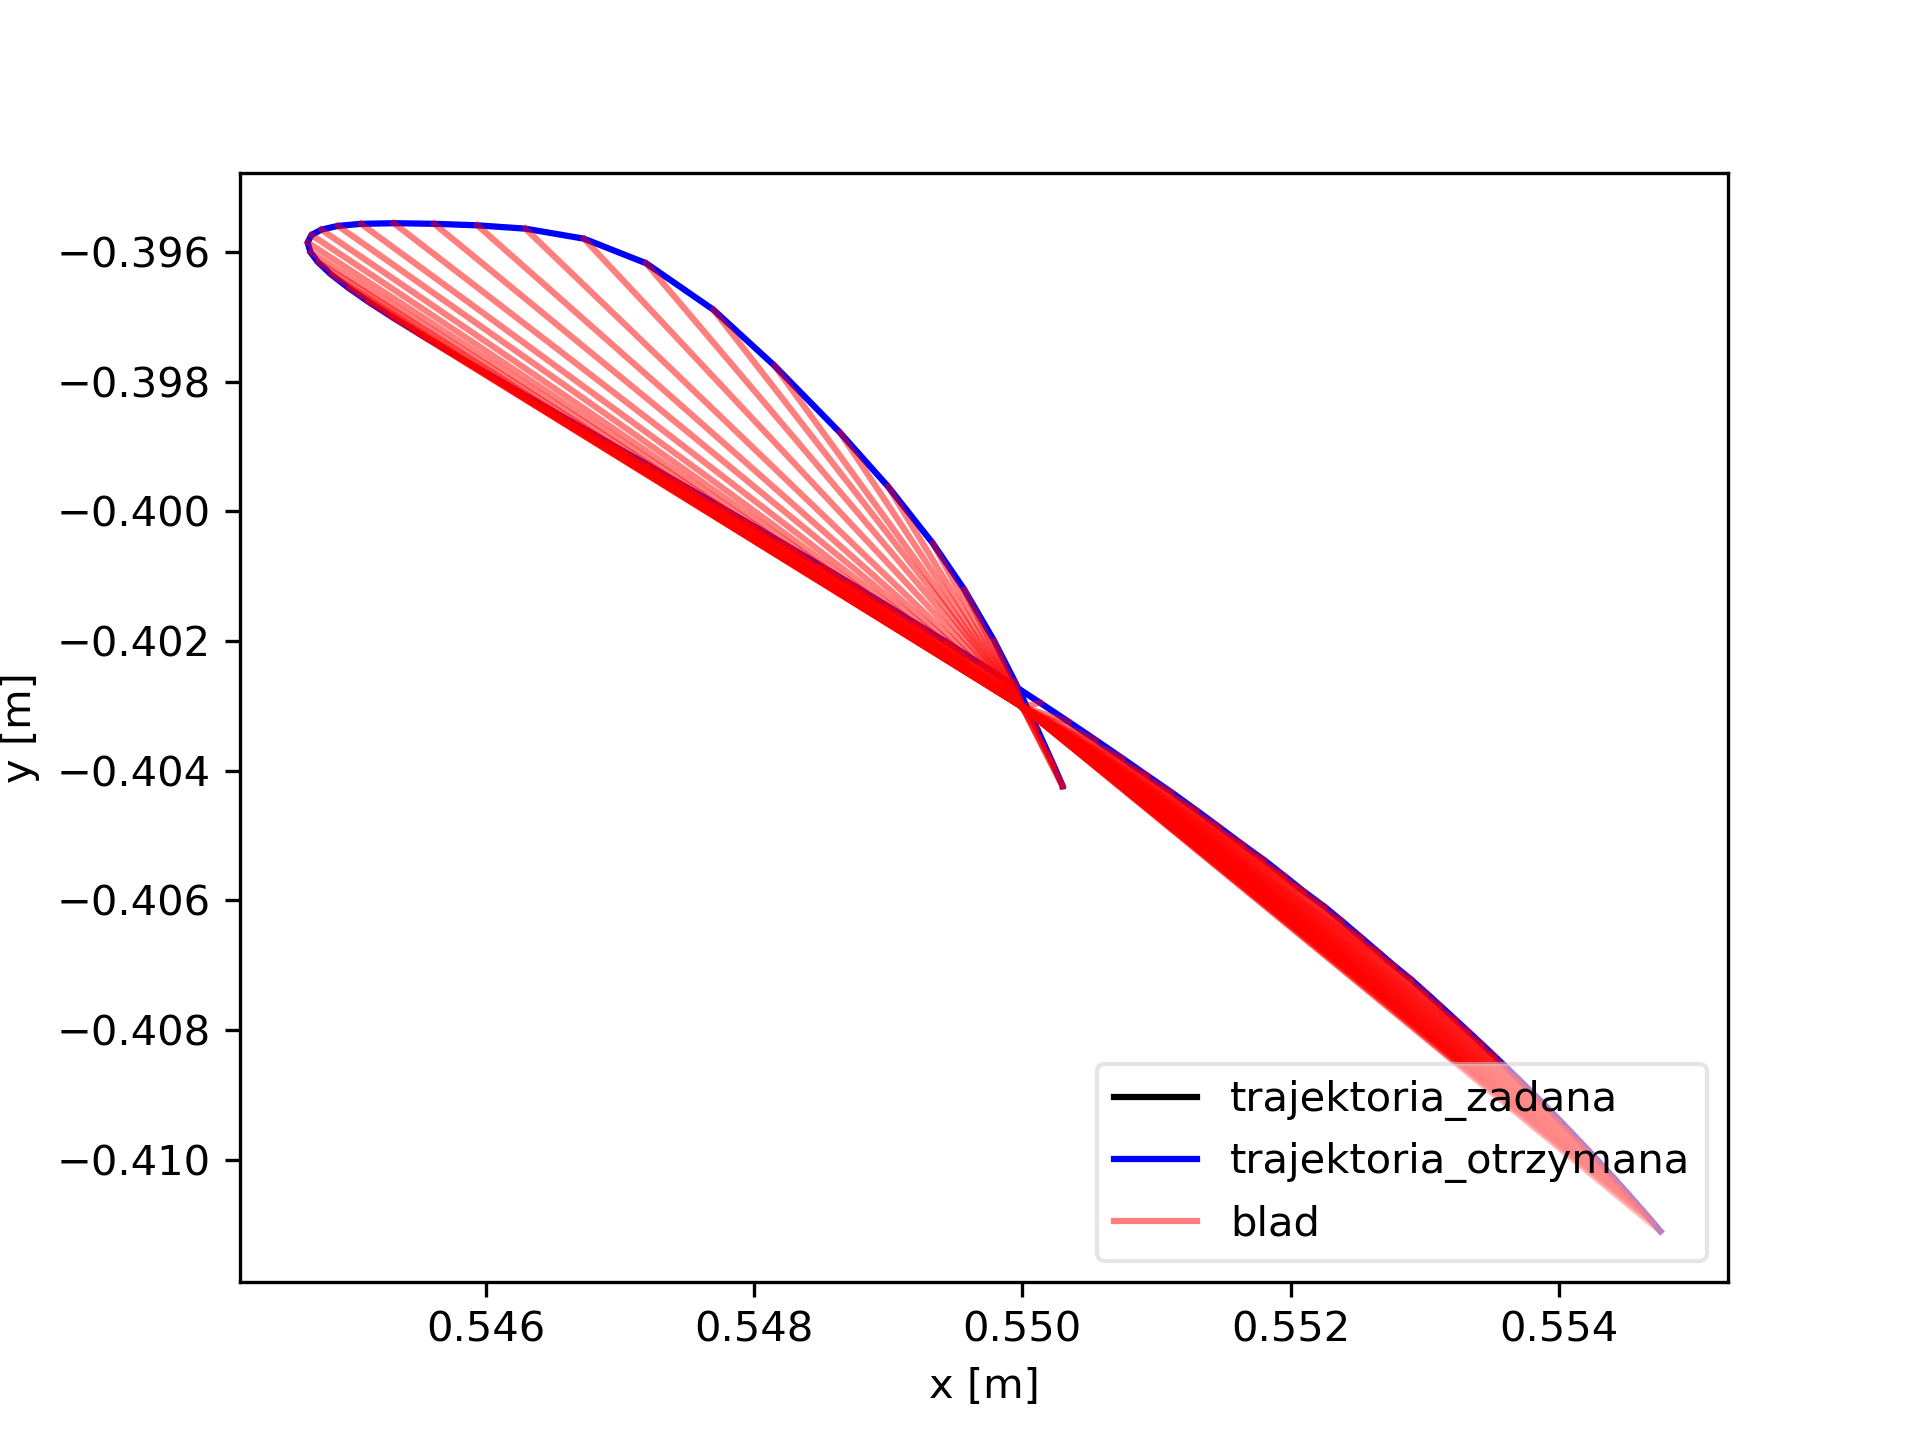
\includegraphics[width=.45\textwidth]{../../velma/przerobione_testy/out/do_gory/xy_ate_plot_podnoszenie_miekki_bez_brak.png}
% 	}
% 	\hfill
% 	\subfigure[Zalaczony algorytm kompnesacji]{
% 		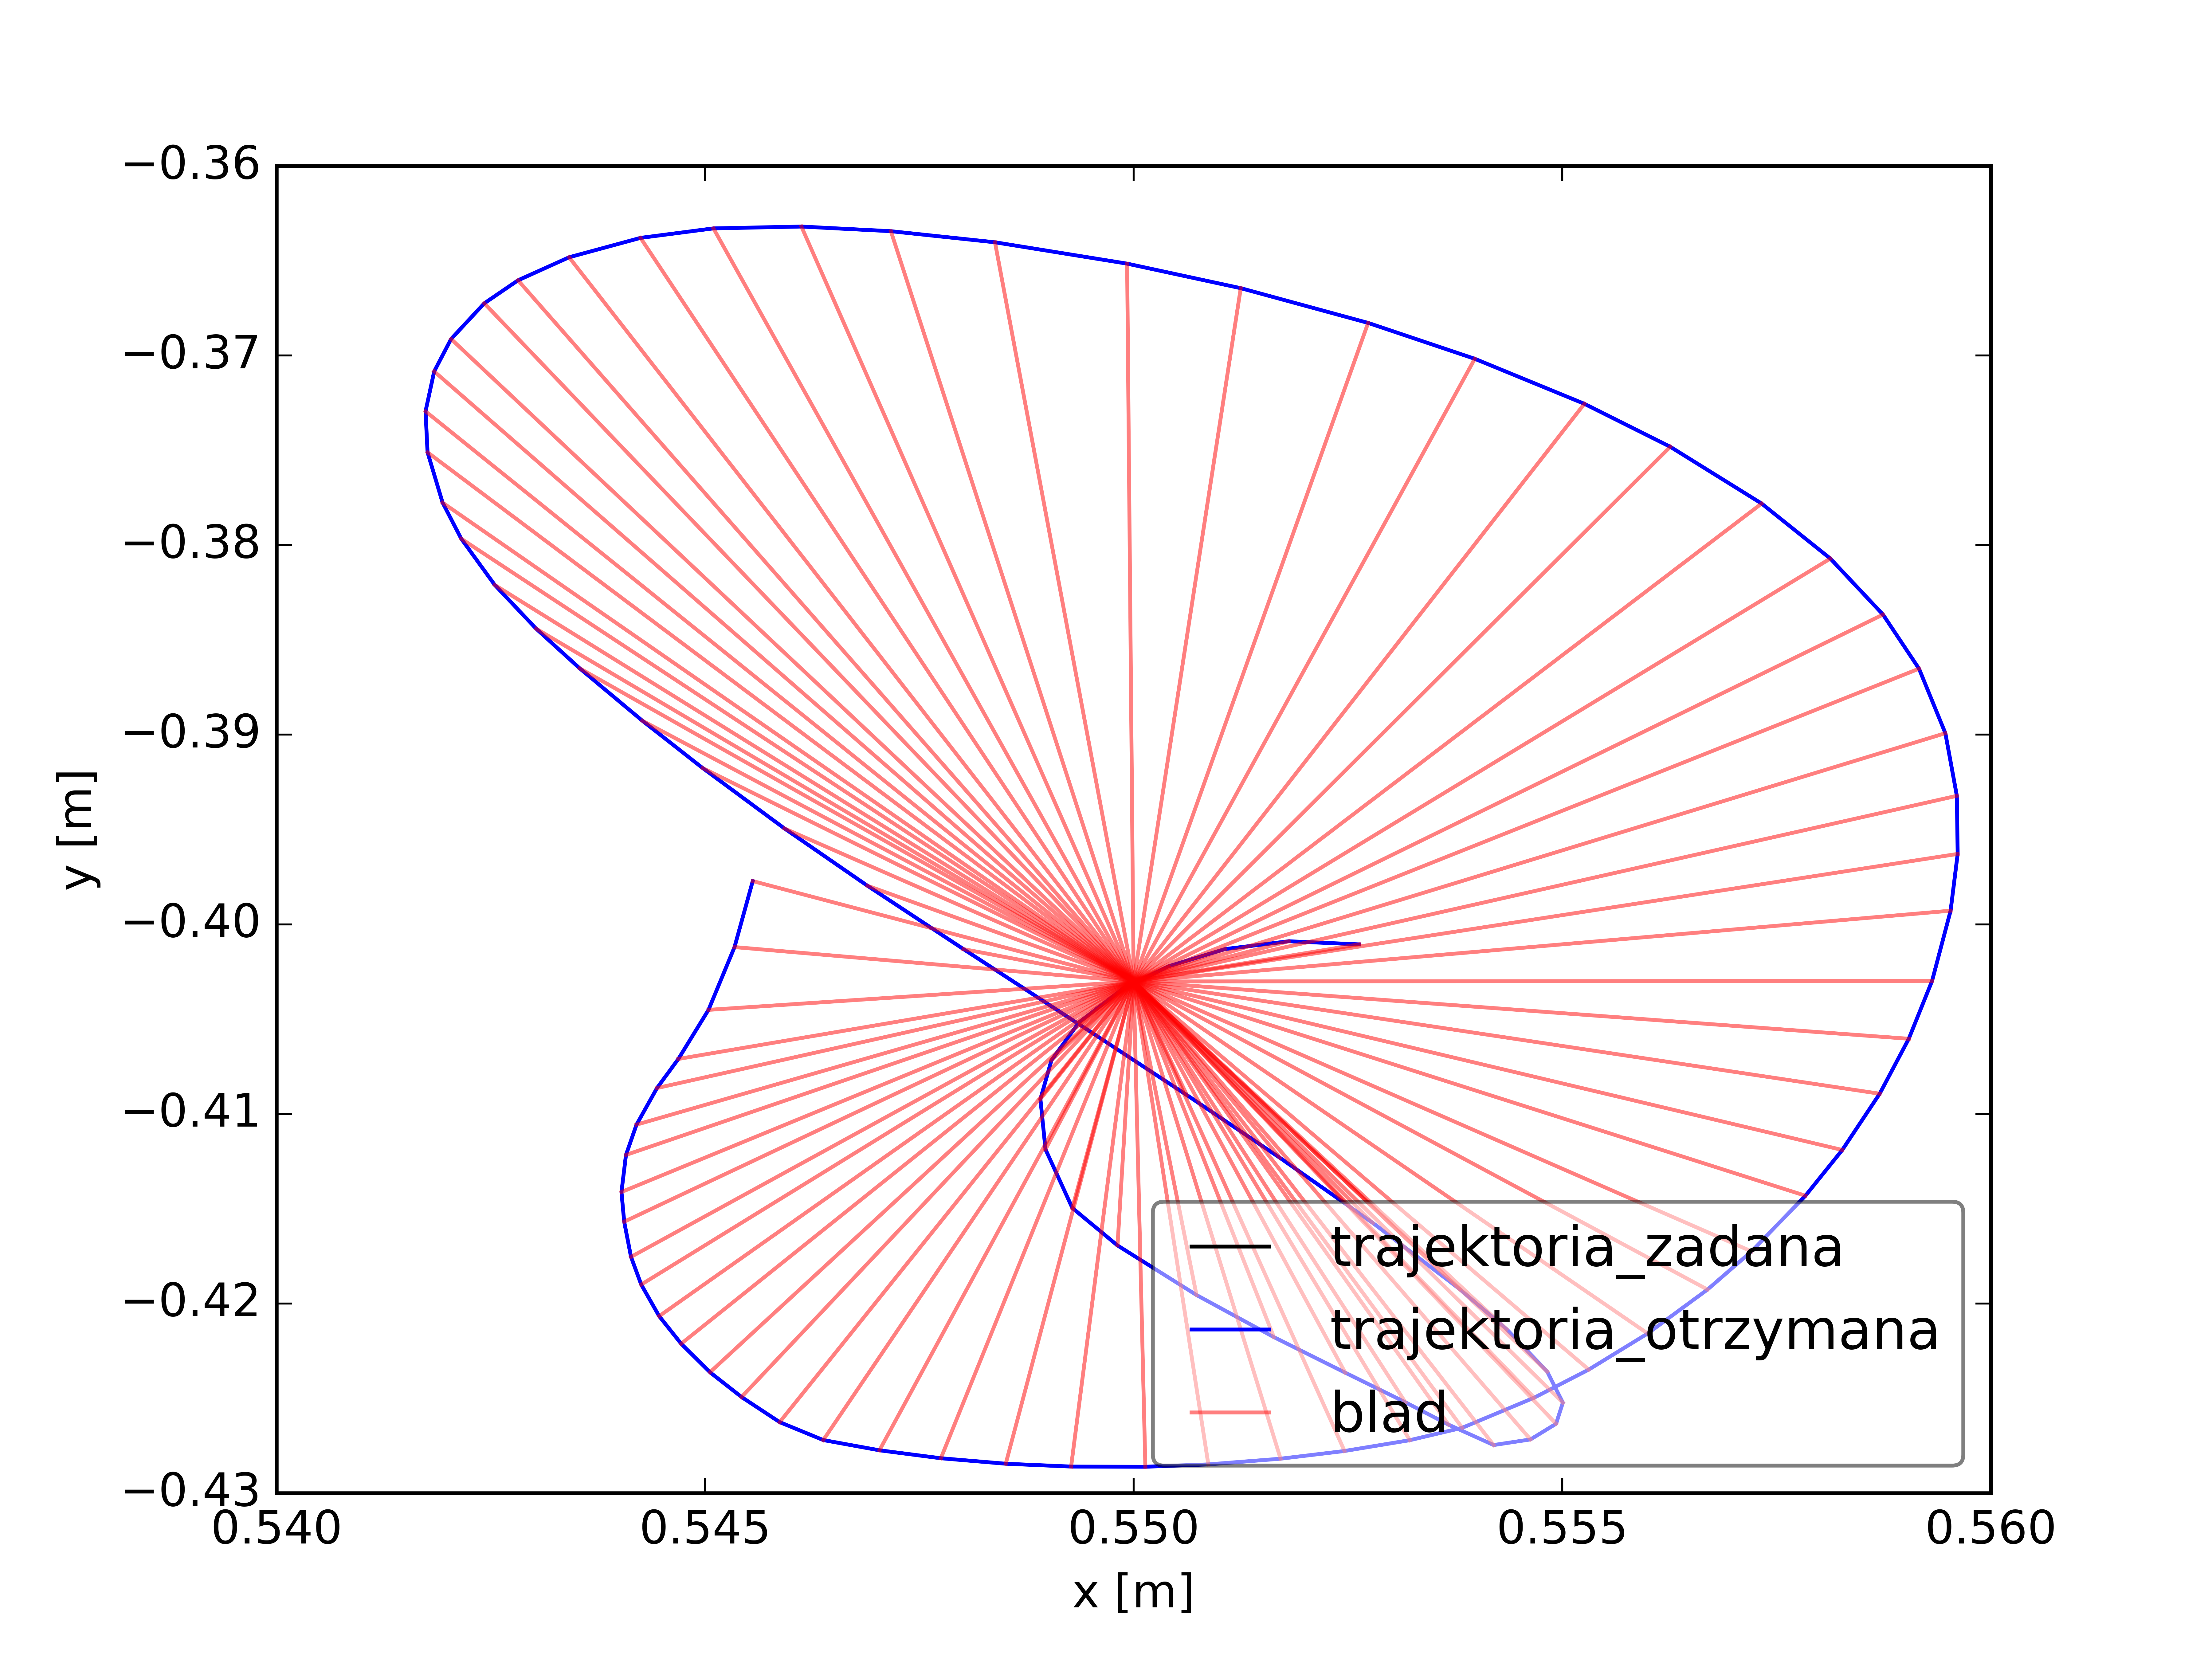
\includegraphics[width=.45\textwidth]{../../velma/przerobione_testy/out/do_gory/xy_ate_plot_podnoszenie_miekki_komp_brak.png}
% 	}
% 	\caption{Porownanie trajektorii chwytaka w osiach $X$ i $Y$}
% 	\label{fig:do_gory_porow_komp_bok}
% \end{figure}

% \begin{figure}
% 	\centering
% 	\subfigure[Trajektoria z chwycona puszka]{
% 		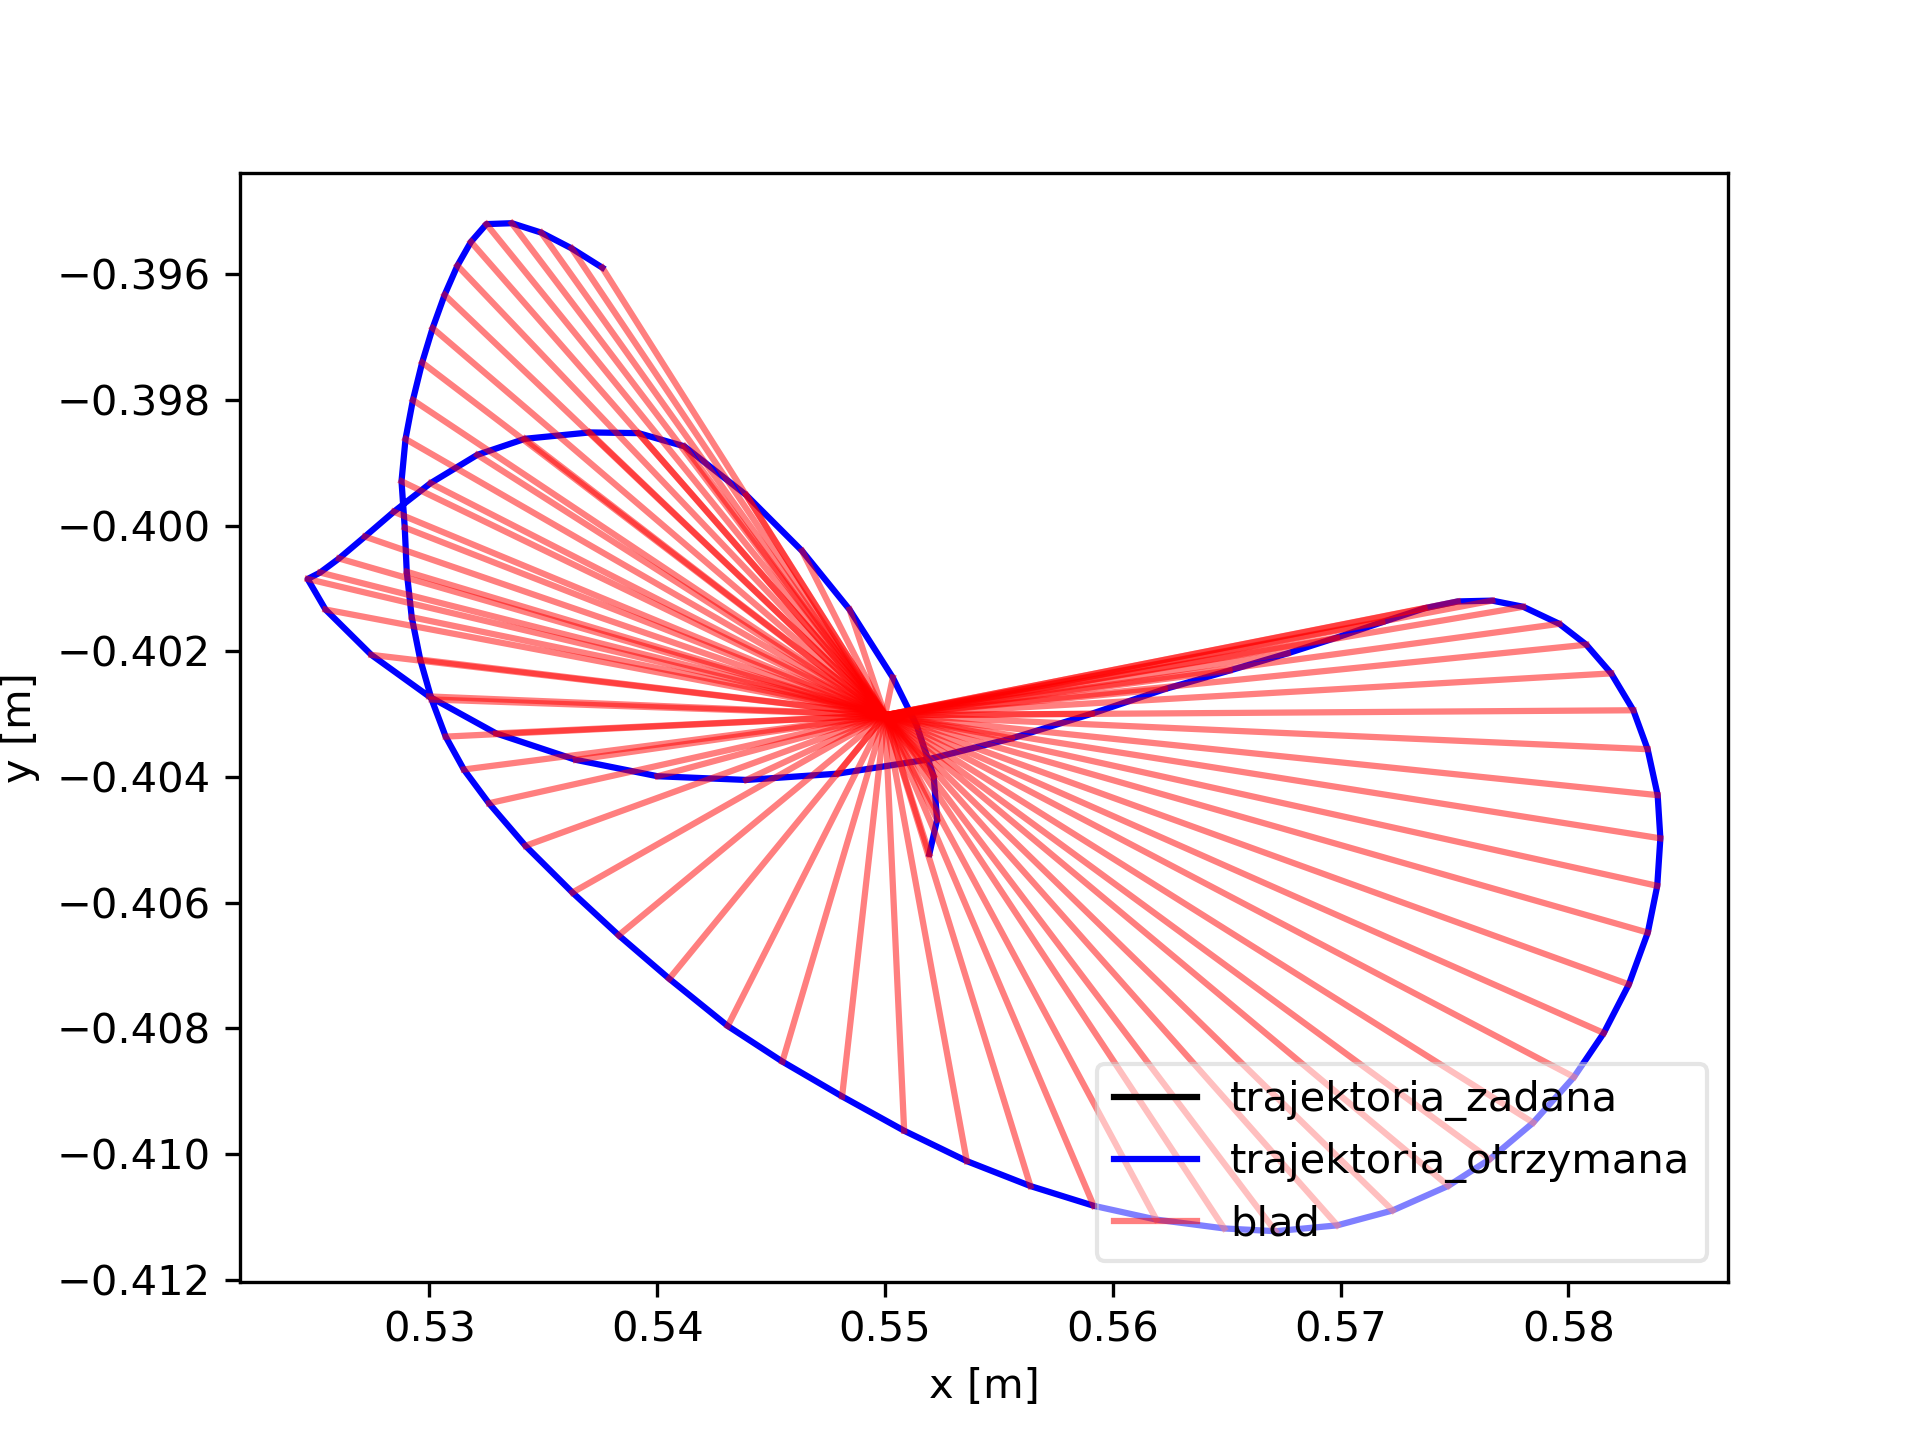
\includegraphics[width=.45\textwidth]{../../velma/przerobione_testy/out/do_gory/xy_ate_plot_podnoszenie_miekki_komp_piwo.png}
% 	}
% 	\hfill
% 	\subfigure[Trajektoria z chwycona wiertarka]{
% 		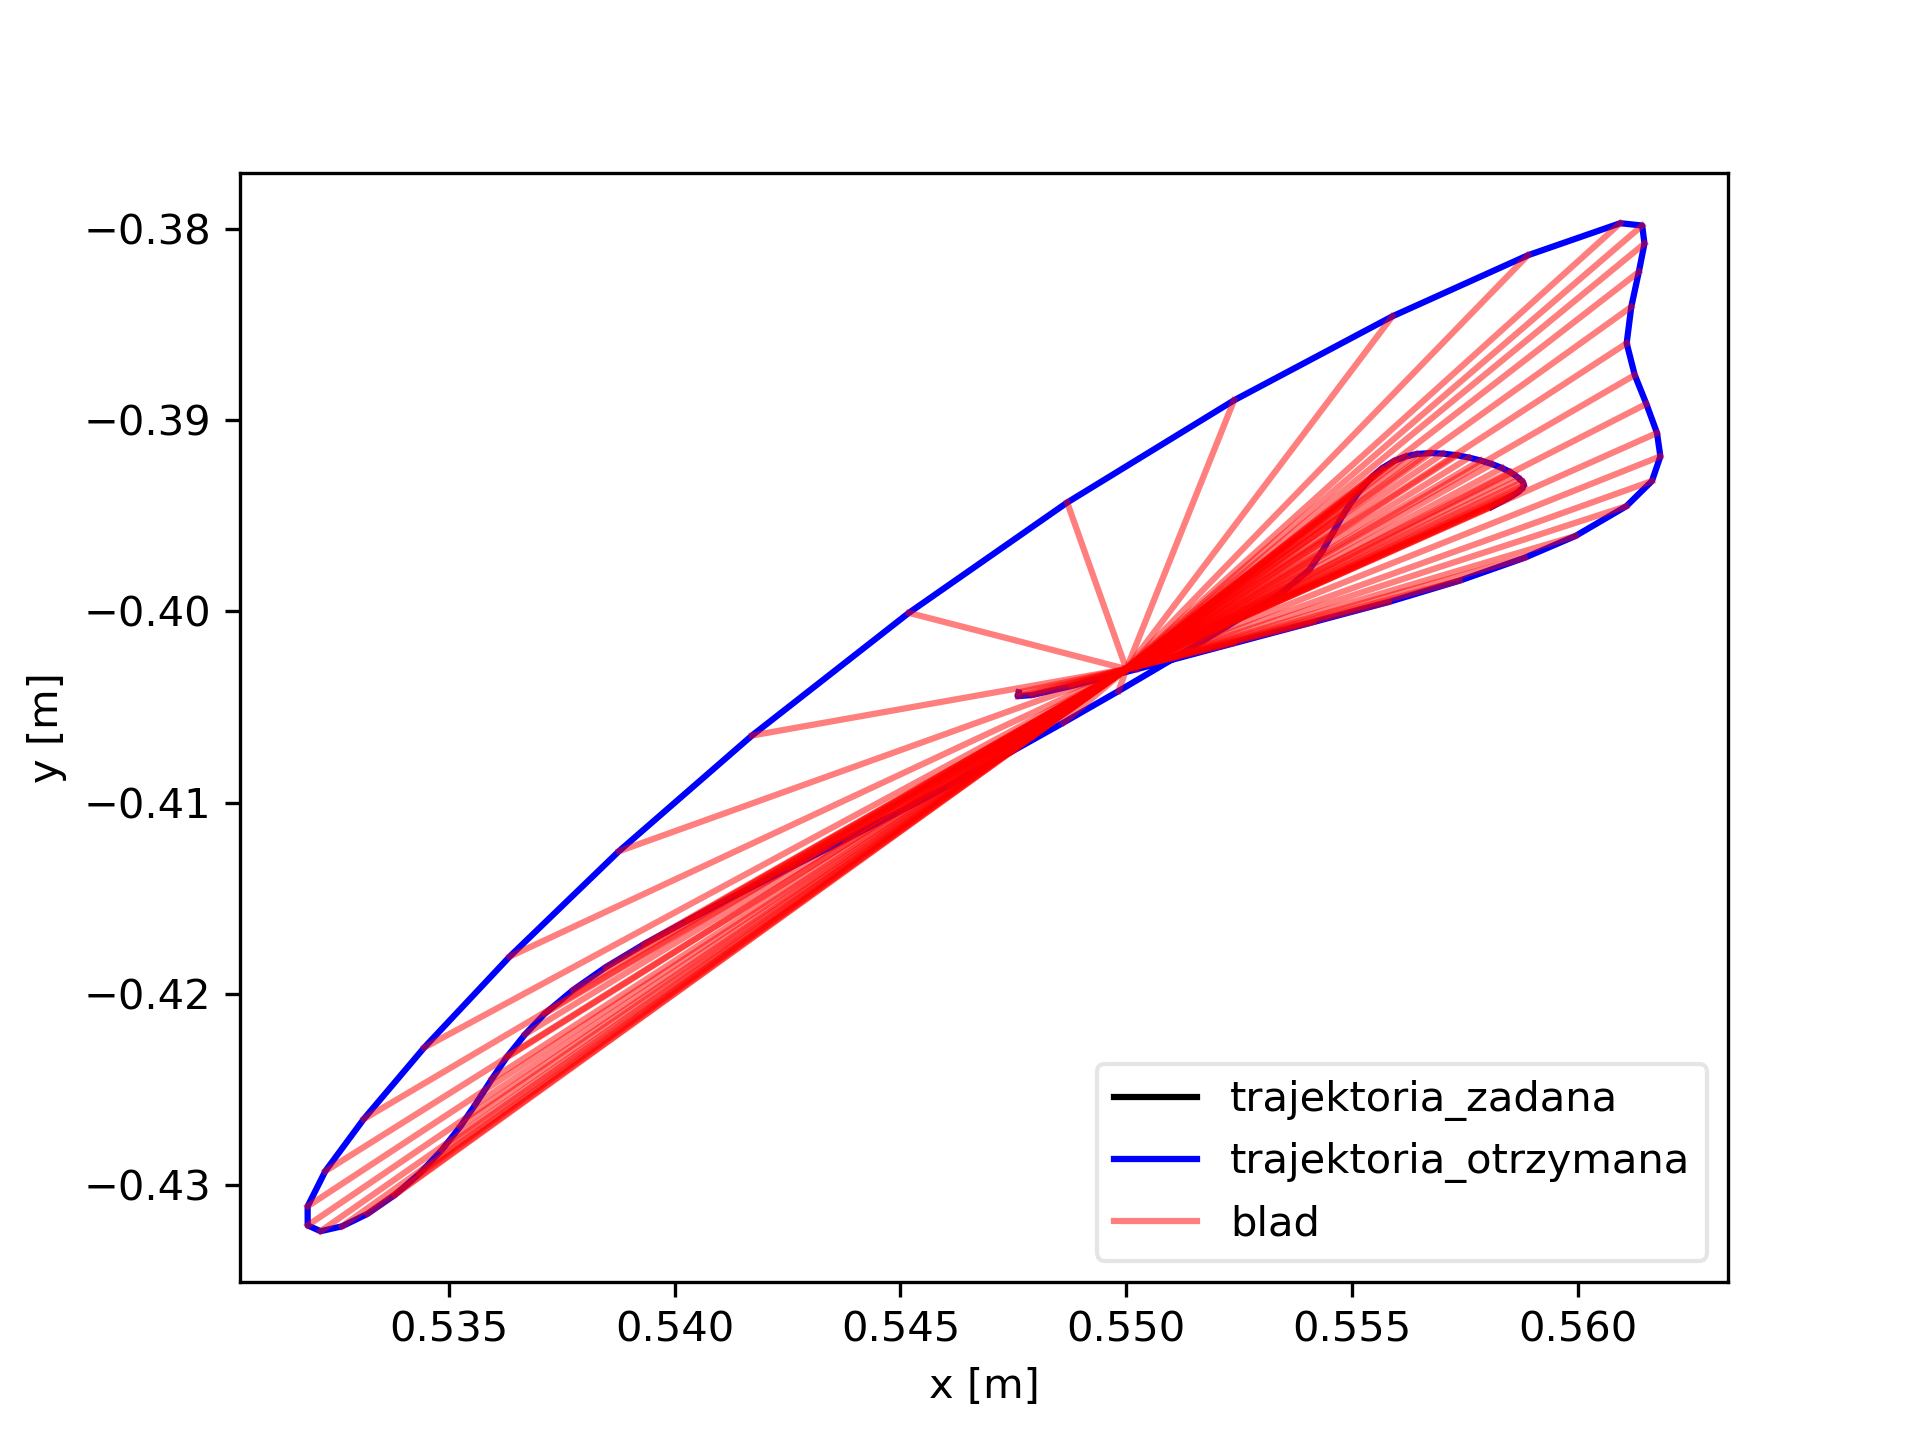
\includegraphics[width=.45\textwidth]{../../velma/przerobione_testy/out/do_gory/xy_ate_plot_podnoszenie_miekki_komp_wiertarka.png}
% 	}
% 	\caption{Porownanie trajektorii chwytaka w osiach $X$ i $Y$}
% 	\label{fig:do_gory_porow_przedm_bok}
% \end{figure}

\begin{figure}[h]
	\centering
	\subfigure[Rzut na wprost]{
		\label{fig:do_gory_porow_zbiorcze_a}
		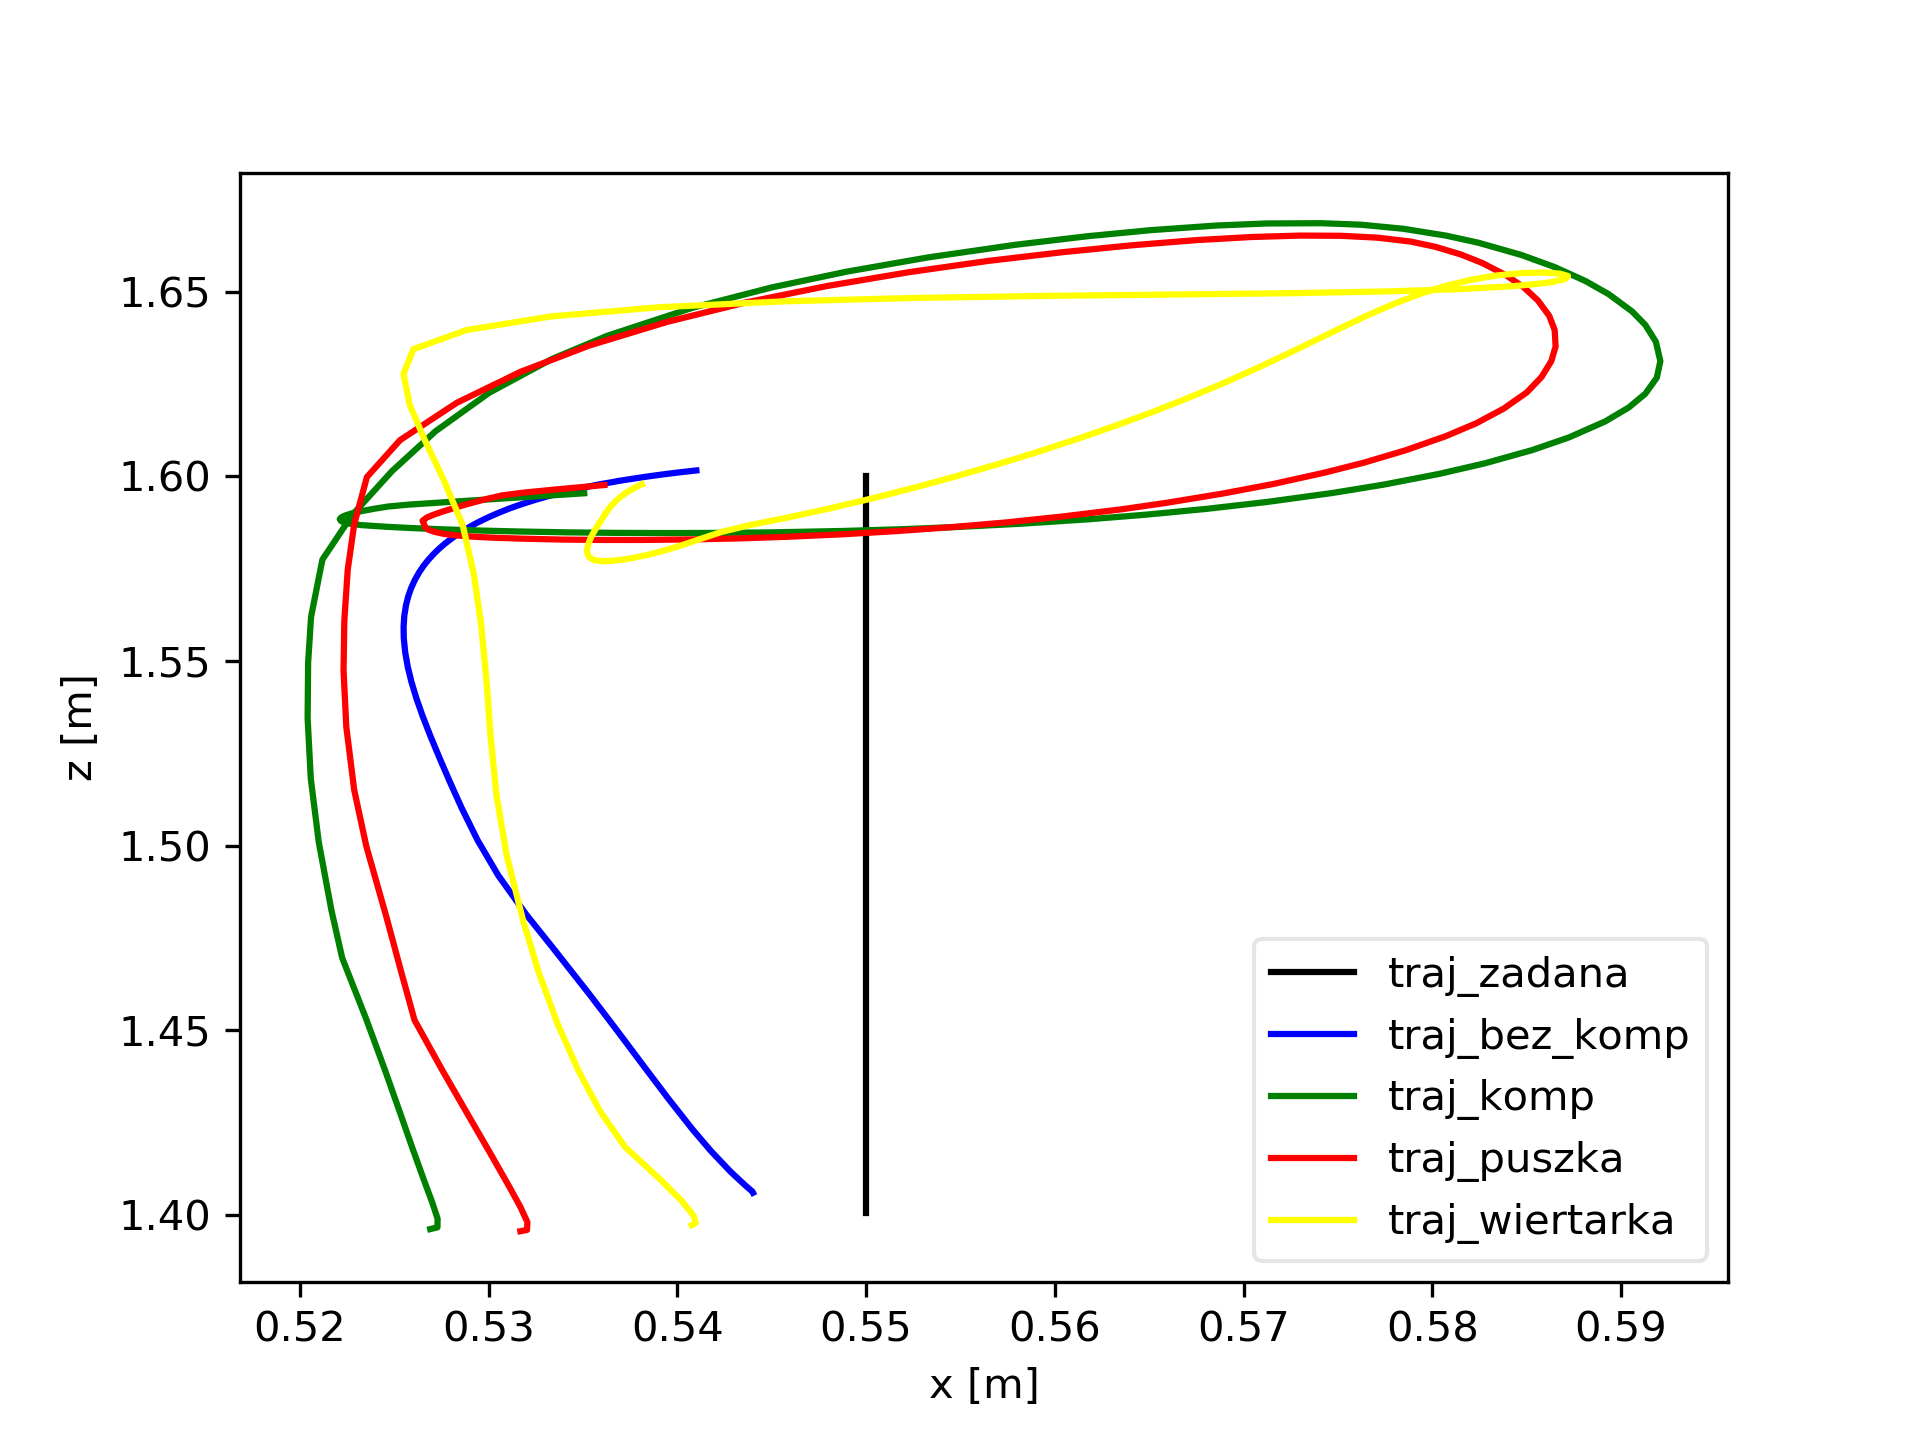
\includegraphics[width=.45\textwidth]{../../velma/przerobione_testy/out/do_gory/common_xz.png}
	}
	% \hfill
	% \subfigure[Rzut z gory]{
	% 	\label{fig:do_gory_porow_zbiorcze_b}
	% 	\includegraphics[width=.45\textwidth]{../../velma/przerobione_testy/out/do_gory/common_xy.png}
	% }
	\caption{Porowanie wszystkich trajektorii.}
	\label{fig:do_gory_porow_zbiorcze}
\end{figure}

\subsection{Ruch do dolu}

Eksperyment ma przetestowac zachowanie algorytmu kompensacji przy ruchu koncowki do dolu (rys. \ref{fig:do_dolu_a}, \ref{fig:do_dolu_rot}). Podobnie jak przy eksperymencie ruchu do gory warty uwagi jest aspekt dzialania sily grawitacji w tej samej co ruch osi. Trajektoria ruchu w rzucie APE na wprost ruchu zostala zaprezentowana na rys. \ref{fig:do__porow_komp}, \ref{fig:do_dolu_porow_przedm} i \ref{fig:do_dolu_porow_zbiorcze_a}. 
% Trajektoria widoczna z boku (w osiach $X$ oraz $Z$) zostala zaprezentowana na rys. \ref{fig:do_dolu_porow_komp_bok}, \ref{fig:do_dolu_porow_przedm_bok} i \ref{fig:do_dolu_porow_zbiorcze_b}.

\begin{figure}[h]
	\centering
	\subfigure[Os $X$]{
		\label{fig:do_dolu_ax}
		\includegraphics[width=.45\textwidth]{../../velma/przerobione_testy/out/do_dolu/common_ax.png}
	}
	\hfill
	\subfigure[Os $Y$]{
		\label{fig:do_dolu_ay}
		\includegraphics[width=.45\textwidth]{../../velma/przerobione_testy/out/do_dolu/common_ay.png}
	}
	
	\hfill
	\subfigure[Os $Z$]{
		\label{fig:do_dolu_az}
		\includegraphics[width=.45\textwidth]{../../velma/przerobione_testy/out/do_dolu/common_az.png}
	}

	\caption{Ruch do dolu. Porownanie trajektorii pozycji w zaleznosci od czasu.}
	\label{fig:do_dolu_a}

\end{figure}


\begin{figure}[h]
	\centering
	\subfigure[Kat osi $X$]{
		\label{fig:do_dolu_rotx}
		\includegraphics[width=.45\textwidth]{../../velma/przerobione_testy/out/do_dolu/common_rotx.png}
	}
	\hfill
	\subfigure[Kat osi $Y$]{
		\label{fig:do_dolu_roty}
		\includegraphics[width=.45\textwidth]{../../velma/przerobione_testy/out/do_dolu/common_roty.png}
	}
	
	\hfill
	\subfigure[Kat osi $Z$]{
		\label{fig:do_dolu_rotz}
		\includegraphics[width=.45\textwidth]{../../velma/przerobione_testy/out/do_dolu/common_rotz.png}
	}

	\caption{Ruch do dolu. Porownanie trajektorii katow w notacji Eulera w zaleznosci od czasu.}
	\label{fig:do_dolu_rot}

\end{figure}


\begin{figure}[h]
	\centering
	\subfigure[Brak algorytmu kompensacji]{
		\includegraphics[width=.45\textwidth]{../../velma/przerobione_testy/out/do_dolu/xz_ate_plot_podnoszenie_miekki_bez_brak.png}
	}
	\hfill
	\subfigure[Zalaczony algorytm kompnesacji]{
		\includegraphics[width=.45\textwidth]{../../velma/przerobione_testy/out/do_dolu/xz_ate_plot_podnoszenie_miekki_komp_brak.png}
	}
	\caption{Porownanie trajektorii chwytaka w osiach $X$ i $Z$}
	\label{fig:do_dolu_porow_komp}
\end{figure}

\begin{figure}[h]
	\centering
	\subfigure[Trajektoria z chwycona puszka]{
		\includegraphics[width=.45\textwidth]{../../velma/przerobione_testy/out/do_dolu/xz_ate_plot_podnoszenie_miekki_komp_piwo.png}
	}
	\hfill
	\subfigure[Trajektoria z chwycona wiertarka]{
		\includegraphics[width=.45\textwidth]{../../velma/przerobione_testy/out/do_dolu/xz_ate_plot_podnoszenie_miekki_komp_wiertarka.png}
	}
	\caption{Porownanie trajektorii chwytaka w osiach $X$ i $Z$}
	\label{fig:do_dolu_porow_przedm}
\end{figure}


% \begin{figure}
% 	\centering
% 	\subfigure[Brak algorytmu kompensacji]{
% 		\includegraphics[width=.45\textwidth]{../../velma/przerobione_testy/out/do_dolu/xy_ate_plot_podnoszenie_miekki_bez_brak.png}
% 	}
% 	\hfill
% 	\subfigure[Zalaczony algorytm kompnesacji]{
% 		\includegraphics[width=.45\textwidth]{../../velma/przerobione_testy/out/do_dolu/xy_ate_plot_podnoszenie_miekki_komp_brak.png}
% 	}
% 	\caption{Porownanie trajektorii chwytaka w osiach $X$ i $Y$}
% 	\label{fig:do_dolu_porow_komp_bok}
% \end{figure}

% \begin{figure}
% 	\centering
% 	\subfigure[Trajektoria z chwycona puszka]{
% 		\includegraphics[width=.45\textwidth]{../../velma/przerobione_testy/out/do_dolu/xy_ate_plot_podnoszenie_miekki_komp_piwo.png}
% 	}
% 	\hfill
% 	\subfigure[Trajektoria z chwycona wiertarka]{
% 		\includegraphics[width=.45\textwidth]{../../velma/przerobione_testy/out/do_dolu/xy_ate_plot_podnoszenie_miekki_komp_wiertarka.png}
% 	}
% 	\caption{Porownanie trajektorii chwytaka w osiach $X$ i $Y$}
% 	\label{fig:do_dolu_porow_przedm_bok}
% \end{figure}

\begin{figure}[h]
	\centering
	\subfigure[Rzut na wprost]{
		\label{fig:do_dolu_porow_zbiorcze_a}
		\includegraphics[width=.45\textwidth]{../../velma/przerobione_testy/out/do_dolu/common_xz.png}
	}
	\hfill
	% \subfigure[Rzut z gory]{
	% 	\label{fig:do_dolu_porow_zbiorcze_b}
	% 	\includegraphics[width=.45\textwidth]{../../velma/przerobione_testy/out/do_dolu/common_xy.png}
	% }
	\caption{Porowanie wszystkich trajektorii.}
	\label{fig:do_dolu_porow_zbiorcze}
\end{figure}

\subsection{Ruch do przodu}

Eksperyment ma przetestowac zachowanie algorytmu kompensacji przy ruchu koncowki w kierunku od robota (rys. \ref{fig:do_przodu_a}, \ref{fig:do_przodu_rot}). Trajektoria ruchu w rzucie na wprost ruchu zostala zaprezentowana na rys. \ref{fig:do_przodu_porow_komp}, \ref{fig:do_przodu_porow_przedm} i \ref{fig:do_przodu_porow_zbiorcze_a}. Trajektoria widoczna z boku (w osiach $X$ oraz $Z$) zostala zaprezentowana na rys. \ref{fig:do_przodu_porow_komp_bok}, \ref{fig:do_przodu_porow_przedm_bok} i \ref{fig:do_przodu_porow_zbiorcze_b}.

\begin{figure}
	\centering
	\subfigure[Os $X$]{
		\label{fig:do_przodu_ax}
		\includegraphics[width=.45\textwidth]{../../velma/przerobione_testy/out/do_przodu/common_ax.png}
	}
	\hfill
	\subfigure[Os $Y$]{
		\label{fig:do_przodu_ay}
		\includegraphics[width=.45\textwidth]{../../velma/przerobione_testy/out/do_przodu/common_ay.png}
	}
	
	\hfill
	\subfigure[Os $Z$]{
		\label{fig:do_przodu_az}
		\includegraphics[width=.45\textwidth]{../../velma/przerobione_testy/out/do_przodu/common_az.png}
	}

	\caption{Ruch do przodu. Porownanie trajektorii pozycji w zaleznosci od czasu.}
	\label{fig:do_przodu_a}

\end{figure}


\begin{figure}
	\centering
	\subfigure[Kat osi $X$]{
		\label{fig:do_przodu_rotx}
		\includegraphics[width=.45\textwidth]{../../velma/przerobione_testy/out/do_przodu/common_rotx.png}
	}
	\hfill
	\subfigure[Kat osi $Y$]{
		\label{fig:do_przodu_roty}
		\includegraphics[width=.45\textwidth]{../../velma/przerobione_testy/out/do_przodu/common_roty.png}
	}
	
	\hfill
	\subfigure[Kat osi $Z$]{
		\label{fig:do_przodu_rotz}
		\includegraphics[width=.45\textwidth]{../../velma/przerobione_testy/out/do_przodu/common_rotz.png}
	}

	\caption{Ruch do przodu. Porownanie trajektorii katow w notacji Eulera w zaleznosci od czasu.}
	\label{fig:do_przodu_rot}

\end{figure}


\begin{figure}
	\centering
	\subfigure[Brak algorytmu kompensacji]{
		\includegraphics[width=.45\textwidth]{../../velma/przerobione_testy/out/do_przodu/xz_ate_plot_podnoszenie_miekki_bez_brak.png}
	}
	\hfill
	\subfigure[Zalaczony algorytm kompnesacji]{
		\includegraphics[width=.45\textwidth]{../../velma/przerobione_testy/out/do_przodu/xz_ate_plot_podnoszenie_miekki_komp_brak.png}
	}
	\caption{Ruch do przodu. Porownanie trajektorii chwytaka w osiach $X$ i $Z$}
	\label{fig:do_przodu_porow_komp}
\end{figure}

\begin{figure}
	\centering
	\subfigure[Trajektoria z chwycona puszka]{
		\includegraphics[width=.45\textwidth]{../../velma/przerobione_testy/out/do_przodu/xz_ate_plot_podnoszenie_miekki_komp_piwo.png}
	}
	\hfill
	\subfigure[Trajektoria z chwycona wiertarka]{
		\includegraphics[width=.45\textwidth]{../../velma/przerobione_testy/out/do_przodu/xz_ate_plot_podnoszenie_miekki_komp_wiertarka.png}
	}
	\caption{Ruch do przodu. Porownanie trajektorii chwytaka w osiach $X$ i $Z$}
	\label{fig:do_przodu_porow_przedm}
\end{figure}


\begin{figure}
	\centering
	\subfigure[Brak algorytmu kompensacji]{
		\includegraphics[width=.45\textwidth]{../../velma/przerobione_testy/out/do_przodu/xy_ate_plot_podnoszenie_miekki_bez_brak.png}
	}
	\hfill
	\subfigure[Zalaczony algorytm kompnesacji]{
		\includegraphics[width=.45\textwidth]{../../velma/przerobione_testy/out/do_przodu/xy_ate_plot_podnoszenie_miekki_komp_brak.png}
	}
	\caption{Porownanie trajektorii chwytaka w osiach $X$ i $Y$}
	\label{fig:do_przodu_porow_komp_bok}
\end{figure}

\begin{figure}
	\centering
	\subfigure[Trajektoria z chwycona puszka]{
		\includegraphics[width=.45\textwidth]{../../velma/przerobione_testy/out/do_przodu/xy_ate_plot_podnoszenie_miekki_komp_piwo.png}
	}
	\hfill
	\subfigure[Trajektoria z chwycona wiertarka]{
		\includegraphics[width=.45\textwidth]{../../velma/przerobione_testy/out/do_przodu/xy_ate_plot_podnoszenie_miekki_komp_wiertarka.png}
	}
	\caption{Porownanie trajektorii chwytaka w osiach $X$ i $Y$}
	\label{fig:do_przodu_porow_przedm_bok}
\end{figure}

\begin{figure}
	\centering
	\subfigure[Rzut na wprost]{
		\label{fig:do_przodu_porow_zbiorcze_a}
		\includegraphics[width=.45\textwidth]{../../velma/przerobione_testy/out/do_przodu/common_xz.png}
	}
	\hfill
	\subfigure[Rzut z gory]{
		\label{fig:do_przodu_porow_zbiorcze_b}
		\includegraphics[width=.45\textwidth]{../../velma/przerobione_testy/out/do_przodu/common_xy.png}
	}
	\caption{Porowanie wszystkich trajektorii bez zaznaczonego bledu.}
	\label{fig:do_przodu_porow_zbiorcze}
\end{figure}


\subsection{Obrot koncowki}

Eksperyment ma przetestowac zachowanie algorytmu kompensacji przy obrocie koncowki. Obserwacje polegaja na zmianie polozen katowych koncowki bez zmiany pozycji. Koncowka ma obrocic sie o zadany kat we wszystkich osiach (rys.\ref{fig:obrt_a}, \ref{fig:obrt_rot}) Trajektoria ruchu (w osiach $X$ oraz $Y$) zostala zaprezentowana na rys. \ref{fig:obrt_porow_komp}, \ref{fig:obrt_porow_przedm} i \ref{fig:obrt_porow_zbiorcze_a}. Trajektoria widoczna z boku (w osiach $X$ oraz $Z$) zostala zaprezentowana na rys. \ref{fig:obrt_porow_komp_bok}, \ref{fig:obrt_porow_przedm_bok} i \ref{fig:obrt_porow_zbiorcze_b}.

\begin{figure}
	\centering
	\subfigure[Os $X$]{
		\label{fig:obrt_ax}
		\includegraphics[width=.45\textwidth]{../../velma/przerobione_testy/out/obrt/common_ax.png}
	}
	\hfill
	\subfigure[Os $Y$]{
		\label{fig:obrt_ay}
		\includegraphics[width=.45\textwidth]{../../velma/przerobione_testy/out/obrt/common_ay.png}
	}
	
	\hfill
	\subfigure[Os $Z$]{
		\label{fig:obrt_az}
		\includegraphics[width=.45\textwidth]{../../velma/przerobione_testy/out/obrt/common_az.png}
	}

	\caption{Porownanie trajektorii pozycji w zaleznosci od czasu.}
	\label{fig:obrt_a}

\end{figure}


\begin{figure}
	\centering
	\subfigure[Kat osi $X$]{
		\label{fig:obrt_rotx}
		\includegraphics[width=.45\textwidth]{../../velma/przerobione_testy/out/obrt/common_rotx.png}
	}
	\hfill
	\subfigure[Kat osi $Y$]{
		\label{fig:obrt_roty}
		\includegraphics[width=.45\textwidth]{../../velma/przerobione_testy/out/obrt/common_roty.png}
	}
	
	\hfill
	\subfigure[Kat osi $Z$]{
		\label{fig:obrt_rotz}
		\includegraphics[width=.45\textwidth]{../../velma/przerobione_testy/out/obrt/common_rotz.png}
	}

	\caption{Porownanie trajektorii katow w notacji Eulera w zaleznosci od czasu.}
	\label{fig:obrt_rot}

\end{figure}


\begin{figure}
	\centering
	\subfigure[Brak algorytmu kompensacji]{
		\includegraphics[width=.45\textwidth]{../../velma/przerobione_testy/out/obrt/xz_ate_plot_podnoszenie_miekki_bez_brak.png}
	}
	\hfill
	\subfigure[Zalaczony algorytm kompnesacji]{
		\includegraphics[width=.45\textwidth]{../../velma/przerobione_testy/out/obrt/xz_ate_plot_podnoszenie_miekki_komp_brak.png}
	}
	\caption{Porownanie trajektorii chwytaka w osiach $X$ i $Z$}
	\label{fig:obrt_porow_komp}
\end{figure}

\begin{figure}
	\centering
	\subfigure[Trajektoria z chwycona puszka]{
		\includegraphics[width=.45\textwidth]{../../velma/przerobione_testy/out/obrt/xz_ate_plot_podnoszenie_miekki_komp_piwo.png}
	}
	\hfill
	\subfigure[Trajektoria z chwycona wiertarka]{
		\includegraphics[width=.45\textwidth]{../../velma/przerobione_testy/out/obrt/xz_ate_plot_podnoszenie_miekki_komp_wiertarka.png}
	}
	\caption{Porownanie trajektorii chwytaka w osiach $X$ i $Z$}
	\label{fig:obrt_porow_przedm}
\end{figure}


\begin{figure}
	\centering
	\subfigure[Brak algorytmu kompensacji]{
		\includegraphics[width=.45\textwidth]{../../velma/przerobione_testy/out/obrt/xy_ate_plot_podnoszenie_miekki_bez_brak.png}
	}
	\hfill
	\subfigure[Zalaczony algorytm kompnesacji]{
		\includegraphics[width=.45\textwidth]{../../velma/przerobione_testy/out/obrt/xy_ate_plot_podnoszenie_miekki_komp_brak.png}
	}
	\caption{Porownanie trajektorii chwytaka w osiach $X$ i $Y$}
	\label{fig:obrt_porow_komp_bok}
\end{figure}

\begin{figure}
	\centering
	\subfigure[Trajektoria z chwycona puszka]{
		\includegraphics[width=.45\textwidth]{../../velma/przerobione_testy/out/obrt/xy_ate_plot_podnoszenie_miekki_komp_piwo.png}
	}
	\hfill
	\subfigure[Trajektoria z chwycona wiertarka]{
		\includegraphics[width=.45\textwidth]{../../velma/przerobione_testy/out/obrt/xy_ate_plot_podnoszenie_miekki_komp_wiertarka.png}
	}
	\caption{Porownanie trajektorii chwytaka w osiach $X$ i $Y$}
	\label{fig:obrt_porow_przedm_bok}
\end{figure}

\begin{figure}
	\centering
	\subfigure[Rzut na wprost]{
		\label{fig:obrt_porow_zbiorcze_a}
		\includegraphics[width=.45\textwidth]{../../velma/przerobione_testy/out/obrt/common_xz.png}
	}
	\hfill
	\subfigure[Rzut z gory]{
		\label{fig:obrt_porow_zbiorcze_b}
		\includegraphics[width=.45\textwidth]{../../velma/przerobione_testy/out/obrt/common_xy.png}
	}
	\caption{Porowanie wszystkich trajektorii bez zaznaczonego bledu.}
	\label{fig:obrt_porow_zbiorcze}
\end{figure}

\begin{figure}
	\centering
	\subfigure[Trajektoria z chwycona puszka]{
		\includegraphics[width=.45\textwidth]{../../velma/przerobione_testy/out/obrt/xy_ate_plot_podnoszenie_miekki_komp_piwo.png}
	}
	\hfill
	\subfigure[Trajektoria z chwycona wiertarka]{
		\includegraphics[width=.45\textwidth]{../../velma/przerobione_testy/out/obrt/xy_ate_plot_podnoszenie_miekki_komp_wiertarka.png}
	}
	\caption{Porownanie trajektorii chwytaka w osiach $X$ i $Y$}
	\label{fig:obrt_porow_przedm_bok}
\end{figure}



\subsection{Ocena jakosci kolizji}
Ocena jakosci kolizji nastepuje poprzez przylozenie skokowych momentow do stawow ramienia oraz obserwacji zachowania robota. Ocena jakosci uginania robota pod wplywem  symulowanej kolizji nastepuje zgodnie z metoda opisana w sekcji \ref{chap:ocenakonaktu}.

\subsection{Podsumowanie}
% encoding: utf8
% !TEX encoding = utf8
% !TeX spellcheck = pl_PL

\chapter{Podsumowanie\label{chap:podsumowanie}}

Zaprezentowana modyfikacja prawa sterowania impedancyjnego w przestrzeni operacyjnej pozwoliła na szybkie i proste rozwiązanie problemu kompensacji grawitacji chwytanego narzędzia. W przyszłości można usprawnić algorytm poprzez dodanie ograniczenia członu całkującego zapożyczonego z prawa sterowania PID. Dzięki takiej modyfikacji nie będzie miało miejsce praktycznie żadne pogorszenie uginania się robota w trakcie kolizji. Jako alternatywę można stosować algorytm który działa tylko w pionowej osi układu. Prawdopodobne jest jednak to, że spowoduje to znaczne pogorszenie jakości osiąganych trajektorii. 

W przyszłości należałoby stworzyć bardziej precyzyjne narzędzia do oceny jakości kolizji robota z otoczeniem.  Zaprezentowana metodyka pracy stanowi dobre podstawy do testowania zupełnie nowych i bardziej wysublimowanych algorytmów.  Dalsze badania mogłyby skupić się na przyjęciu uproszczonego modelu robota wraz z narzędziem oraz estymacji jego parametrów z wykorzystaniem czujnika FTS i wyliczonych pozycji końcówki.

\bibliographystyle{plplain}
\bibliography{bibliography}

\listoffigures
\listoftables

\end{document}
